\chapter{Plugin functions}
\label{ch:plugins}

%%%%%%%%%%%%%%%%%%%%%%%%%%%%%%%%%%%%%%%%%%%%%%%%%%%%%%%%%%%%%%%%%%%%%%%%%

%\clearpage
\section{Very anisotropic particles (local planar \& local cylindrical objects)}

For very anisotropic random orientated particles the form factor
can be factorize according to Porod \cite{Porod1948} in a cross
section term $P_\text{cs}(Q)$ for the shorter dimension and a
shape factor $P'(Q)$ for the long dimension.
\begin{align}
I(Q) &=P'(Q) P_{cs}(Q).
\end{align}
In this plugin the form factors of two types of anisotropic
particles are collected, those with a local cylindrical and with a
local planar geometry. In case of local planar objects the cross
section term $P_\text{cs}(Q)$ can be homogeneous, a
centro-symmetric bilayer, a gaussian bilayer, etc. . This cross
section factor can than be combined with the overall shape factor
$P'(Q)$ of for examples a thin spherical shell of elliptical
shell, a thin cylindrical shell or a thin disc. As the total form
factor is the product of the cross-section form factor and a shape
form factor one can either programm all combination of
cross-section and shape factors into individual form factor
functions or one can programm the cross-section factors as form
factor and the shape factor as a structure factors. Using the
monodisperse approximation yields than the same result.

In this plugin the product of the cross-section and shape term
have been implemented as form factor under "\texttt{[by
plugin|anisotropic obj.|local planar obj.]}" and "\texttt{[by
plugin|anisotropic obj.|local cylindrical obj.]}". The
cross-section terms alone are also implemented as form factors
under "\texttt{[by plugin|anisotropic obj.|Pcs(Q) for planar obj.]}"
and "\texttt{[by plugin|anisotropic obj.|Pcs(Q) for cylindrical
obj.]}". The shape factors are also available as structure factors
under "\texttt{[by plugin|anisotropic obj.|P'(Q): local planar
obj.]}" and "\texttt{[by plugin|anisotropic obj.|P'(Q): local
cylindrical obj.]}".

The cross-section form factors can be easily calculated if the
scattering length density contrast profile
$\Delta\eta_\textrm{cs}(r)$ is known. For structures with a local
planar geometry and a symmetric cross-section the form factor is
given by
\begin{align}
P_\textrm{cs}^\textrm{planar} (Q) = \left[2\int_0^\infty
\Delta\eta_\textrm{cs}(r) \cos(Qr) \, \textrm{d}r\right]^2
\label{Pcs:planar}
\end{align}
In case of local cylindrical particles with a centro-symmetric
scattering length density distribution the form factor is given by
\begin{align}
P_\textrm{cs}^\textrm{cylindrical} (Q) = \left[2\pi\int_0^\infty
\Delta\eta_\textrm{cs}(r) \textrm{J}_0(Qr)r \,
\textrm{d}r\right]^2 \label{Pcs:cylindrical}
\end{align}

\clearpage
\subsection{Pcs(Q) for planar obj.} ~\\
\label{plugin:Pcs4planar}

The cross-section form factors with local planar geometry are valid
when the cross-section dimension is much smaller the radius of curvature
of the locally planar structure.
\begin{figure}[htb]
\begin{center}
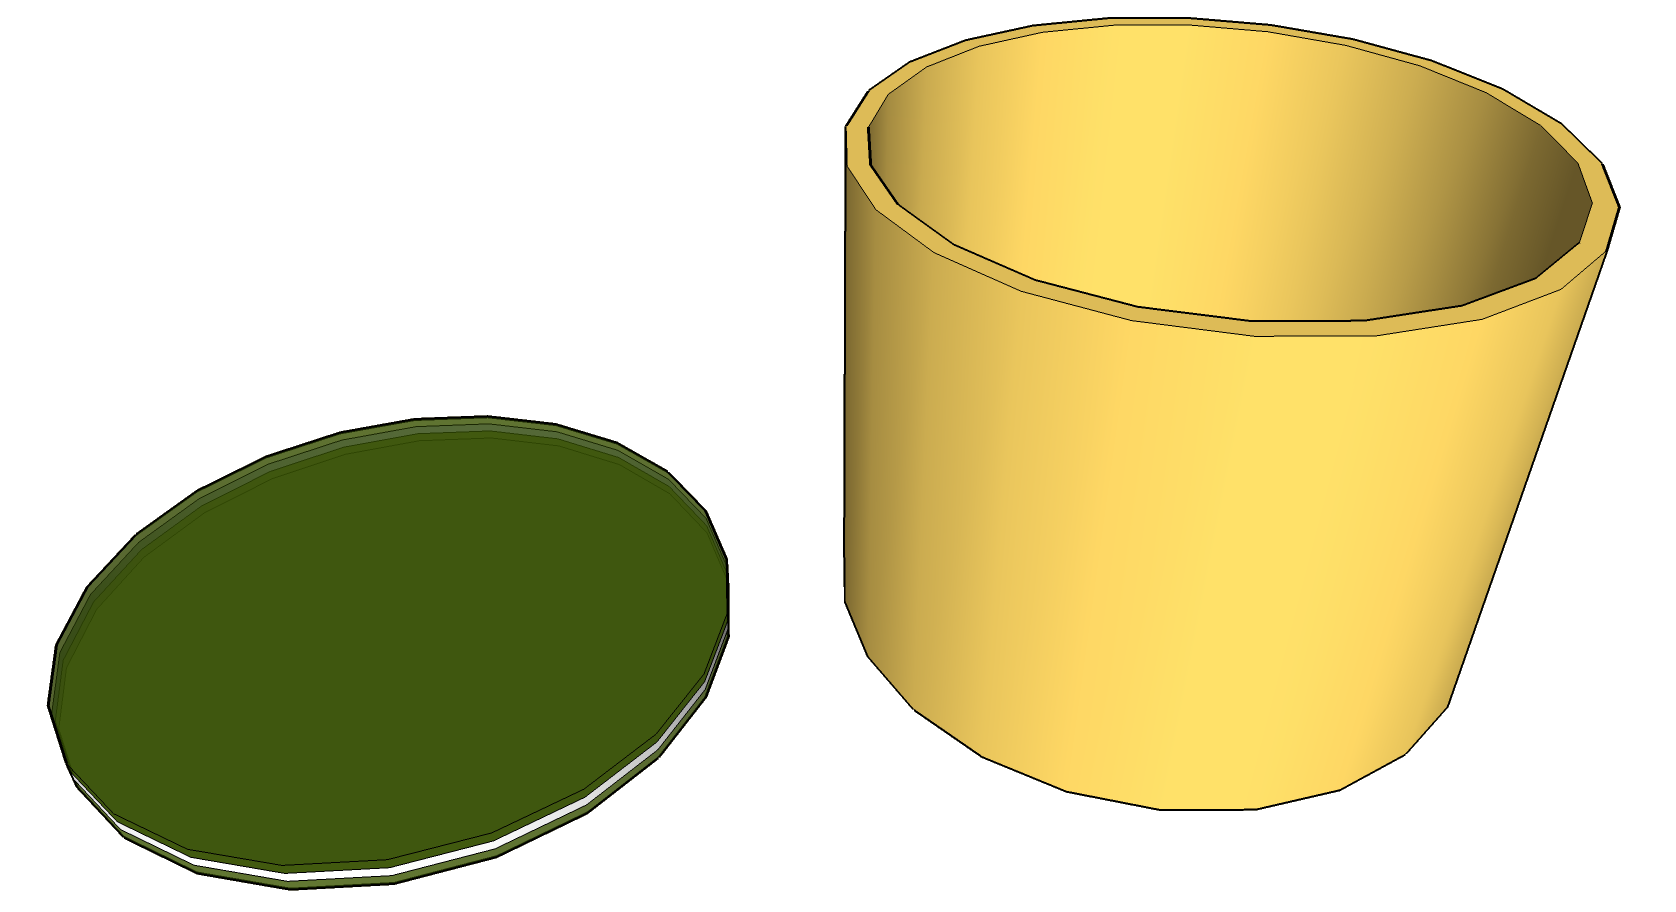
\includegraphics[width=0.838\textwidth,height=0.456\textwidth]{../images/form_factor/anisotropic/localplanar.png}
\end{center}
\caption{for local planar particles the cross section dimension is much smaller then the
radius of curvature of the particle}
\label{fig:localplanar}
\end{figure}

Several cross-section profiles for local planar objects have been implemented,
like a homogeneous cross-section,
cross-section with two infinitely thin plates,
layered centro-symmetric cross-section,
bilayer with a Gaussian scattering length density profile,
layer with Gaussian chains attached to the surface.
These form factors are supposed to be combined with a shape factor for
local planar objects which are implemented as structure  plugins
under "\texttt{[by plugin|anisotropic obj.|P'(Q): local planar
obj.]}".

\clearpage

\subsubsection{Pcs(Q) for a homogeneous cross-section}
\label{plugin:Pcs:homogeneousXS} ~\\

\begin{figure}[htb]
\begin{center}
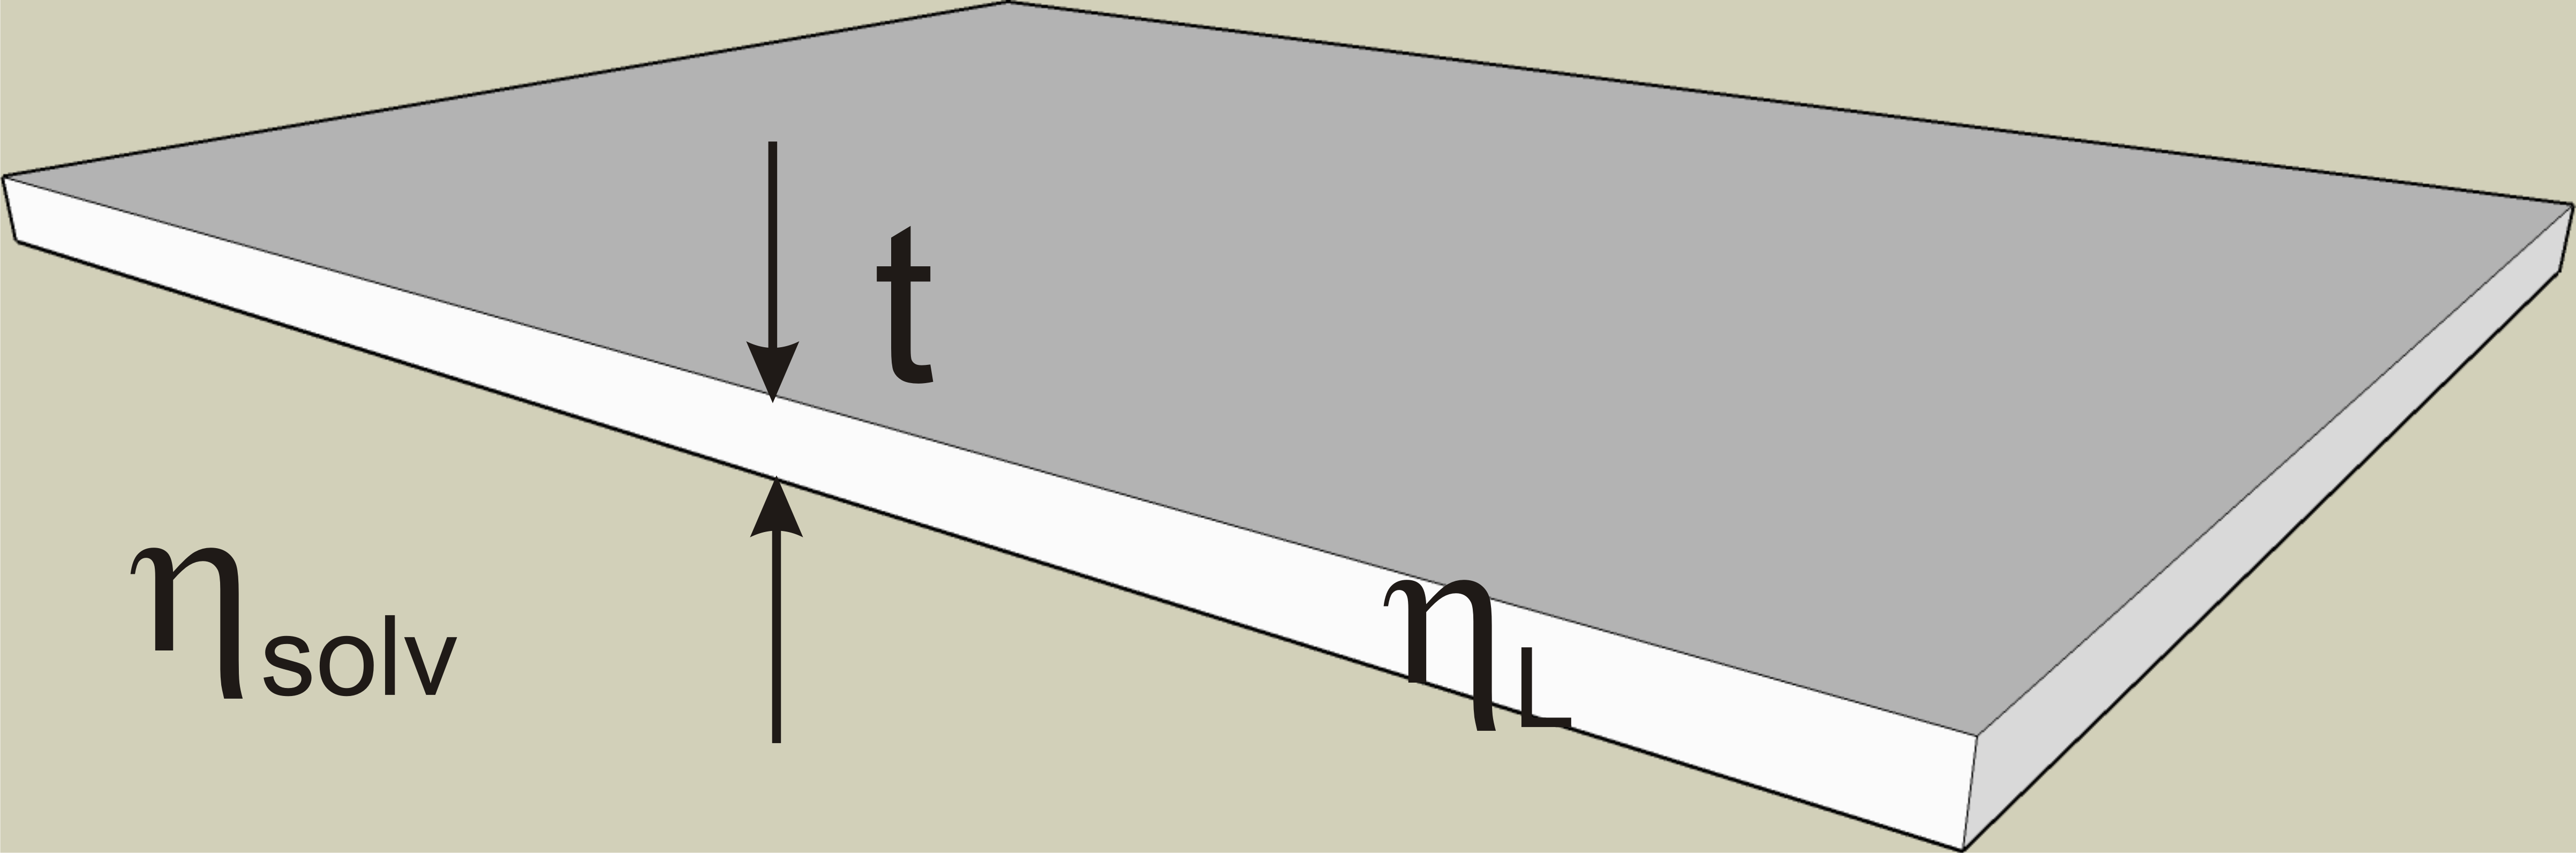
\includegraphics[width=0.802\textwidth,height=0.265\textwidth]{../images/form_factor/anisotropic/Pcs_homogeneousXS_txt.png}
\end{center}
\caption{Plane with a homogeneous cross-section of thickness $t$.}
\label{fig:homogeneousXS}
\end{figure}

This cross-section form factor describes the scattering of a layer with homogeneous
scattering length density $\eta_L$ in a matrix of a scattering length density $\eta_\textrm{solv}$.
The thickness can have a distribution described by a log-normal distribution according to eq.\ \ref{eq:LogNormal}.

\begin{align}
P_\text{cs}(Q,\sigma_{t},t) = \int_0^\infty \textrm{LogNorm}(x,1,\sigma_{t},1,t)
    \left[ \left(\eta_L-\eta_\textrm{solv}\right) x \frac{\sin(Qx/2)}{Qx/2} \right]^2\textrm{d}x
\end{align}

\noindent
\textbf{Input parameters for \texttt{Pcs:homogeneousPlate}:}
\begin{description}
    \item[\texttt{t}] most probable layer thickness $t$
    \item[\texttt{sigm\_t}] width $\sigma_t$ of thickness distribution (LogNorm)
    \item[\texttt{dummy}] unused disabled parameter
    \item[\texttt{dummy}] unused disabled parameter
    \item[\texttt{eta\_l}] scattering length density of layer $\eta_L$
    \item[\texttt{eta\_solv}] scattering length density of solvent $\eta_\textrm{solv}$
\end{description}

\noindent
\textbf{Note}
\begin{itemize}
  \item This form factor is supposed to be combined with a shape factor for
local planar objects which are implemented as structure  plugins
under "\texttt{[by plugin|anisotropic obj.|P'(Q): local planar
obj.]}".
\item As the form factor already have the width distribution included one normally uses in \SASfit as a size distribution
the \texttt{Delta}-distribution.
\end{itemize}

\begin{figure}[htb]
\begin{center}
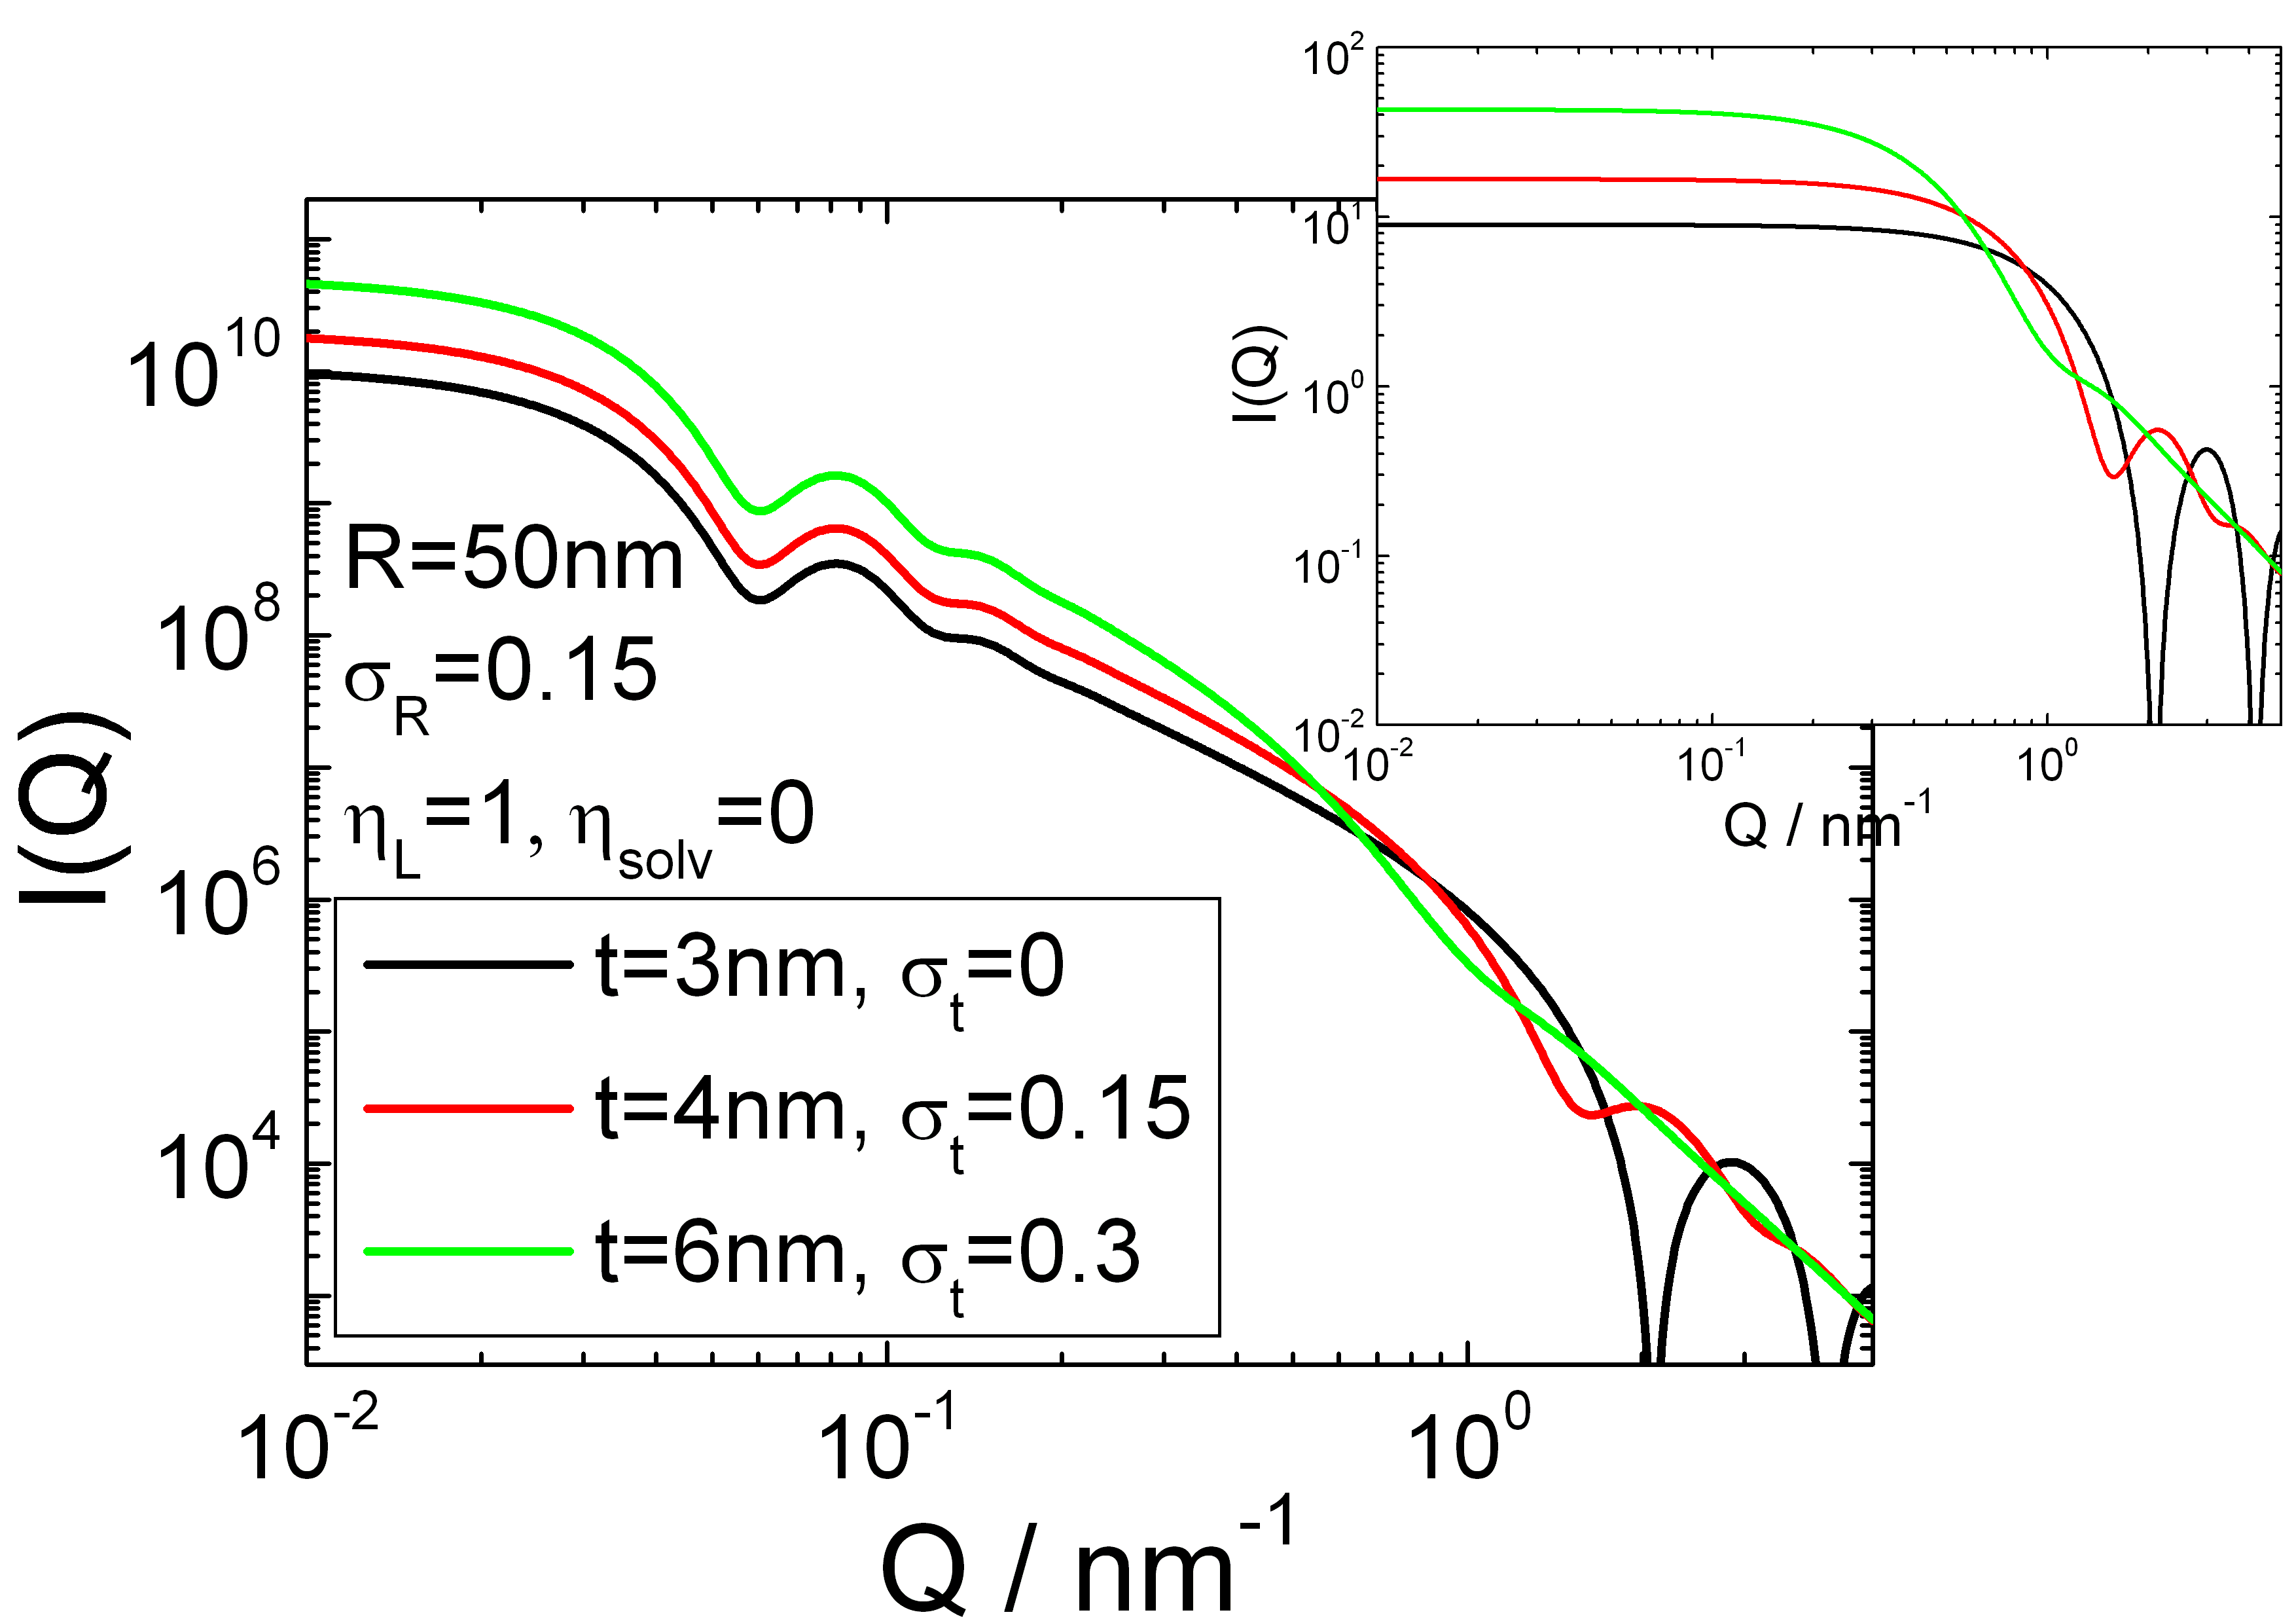
\includegraphics[width=0.8\textwidth,height=0.55\textwidth]{../images/form_factor/anisotropic/localplanarIQ.png}
\end{center}
\caption{Scattering curve for the form factor "\texttt{Pcs:homogeneousPlate}" only (insert) and
in combination with a structure factor "\texttt{P'(Q): Thin Spherical Shell}".}
\label{fig_IQ:homogeneousXS}
\end{figure}

\clearpage
\subsubsection{Pcs(Q) for two infinitely thin parallel layers} ~\\
\label{plugin:Pcs:TwoInfinitelyThinLayers}

\begin{figure}[htb]
\begin{center}
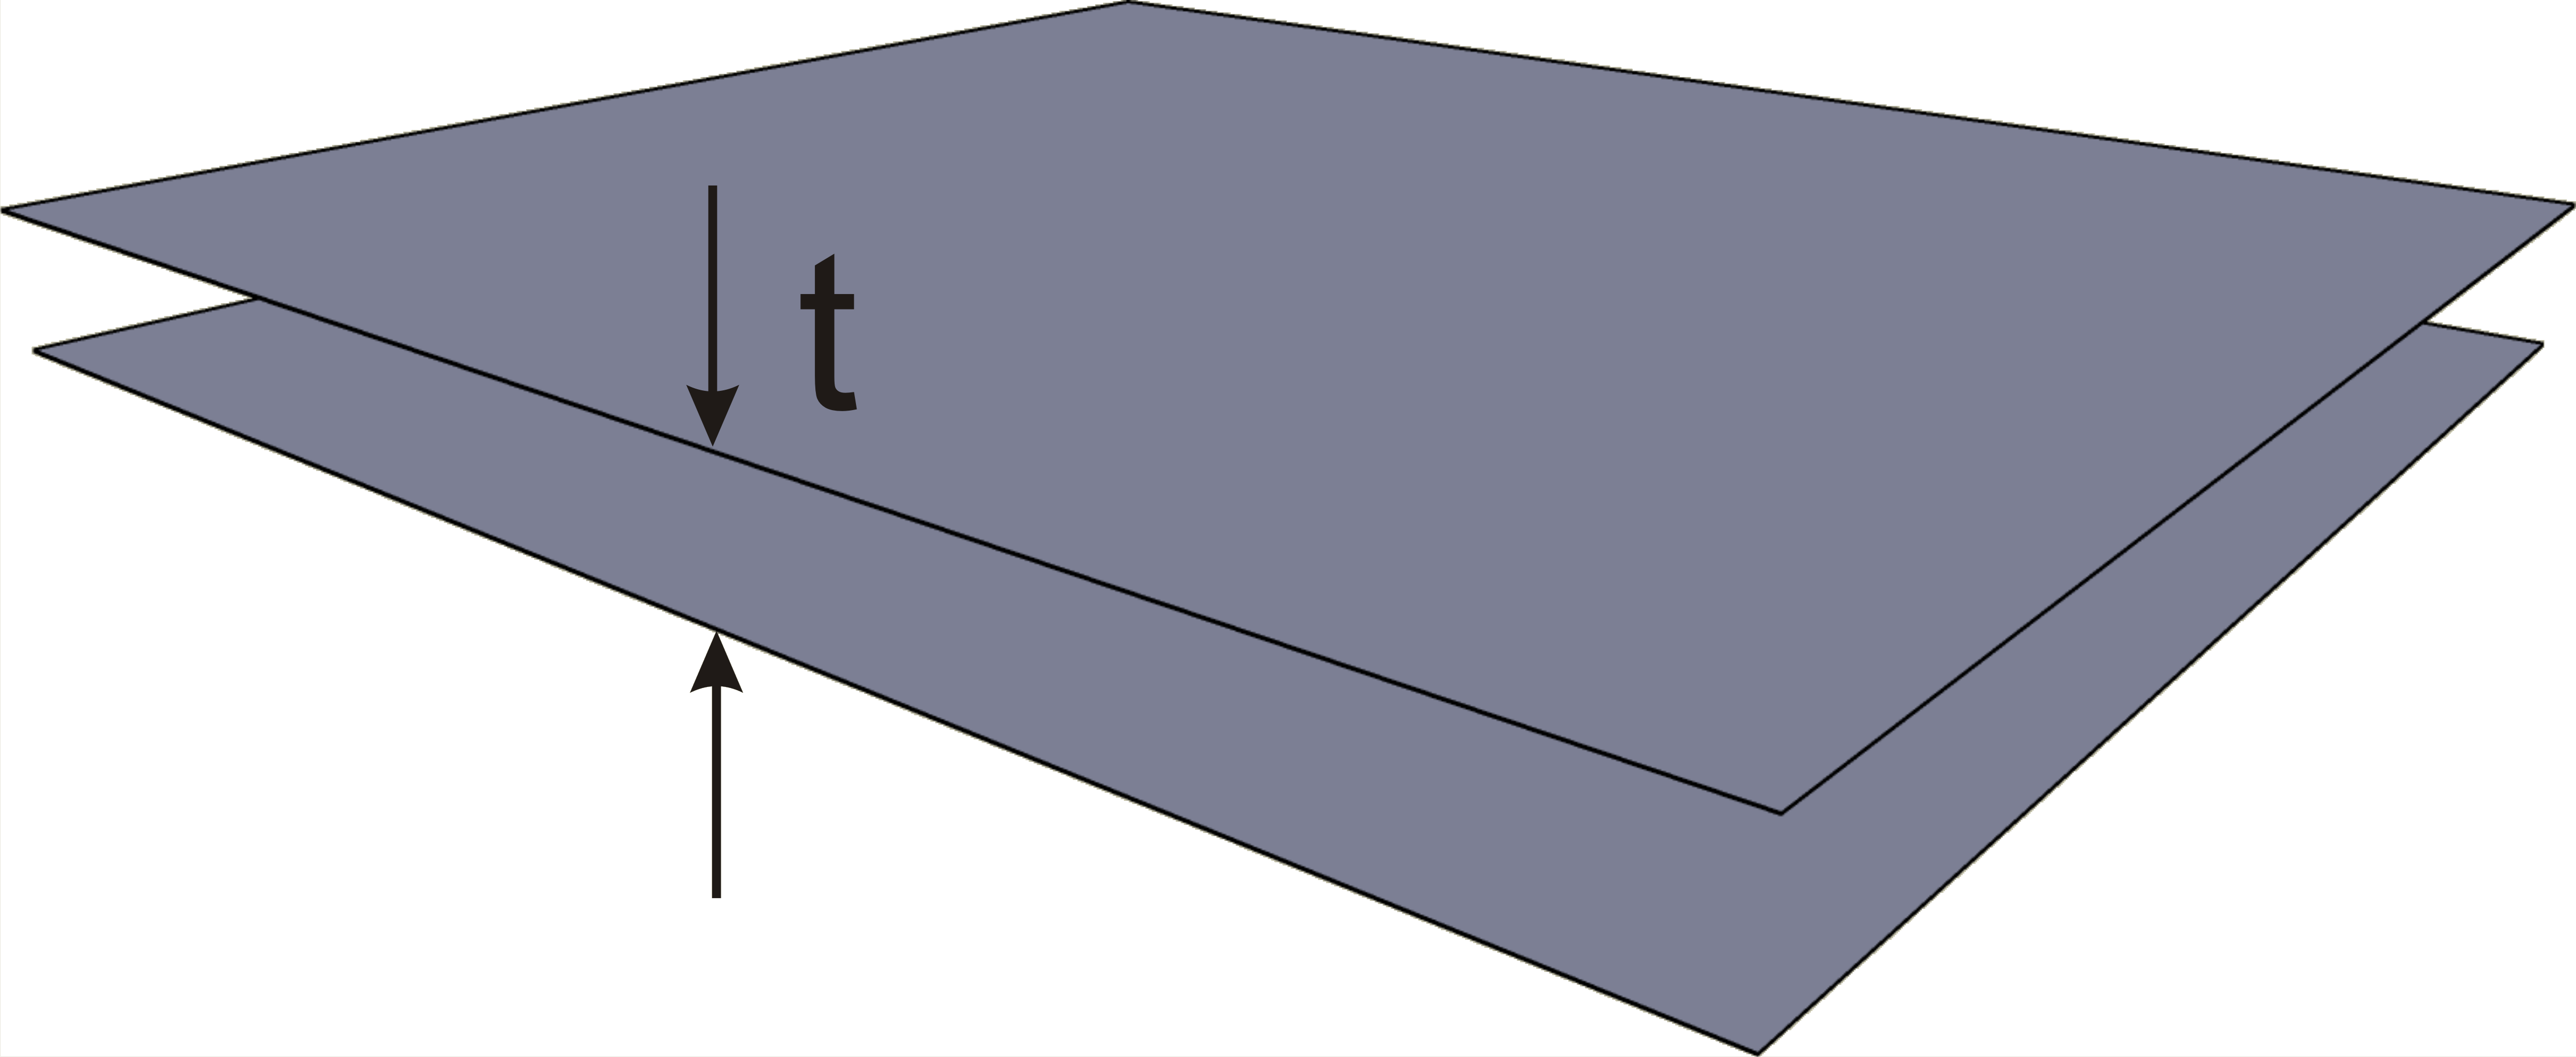
\includegraphics[width=0.8\textwidth,height=0.328\textwidth]{../images/form_factor/anisotropic/planar2thin_txt.png}
\end{center}
\caption{Two infinitely thin parallel layers separated by a distance $t$.}
\label{fig:Pcs:TwoInfinitelyThinLayers}
\end{figure}

This cross-section form factor describes the scattering of two infinitely thin parallel layers.
The separation distance can have a distribution described by a log-normal distribution according
to eq.\ \ref{eq:LogNormal}.

\begin{align}
P_\text{cs}(Q,\sigma_{T},T) = \int_0^\infty \textrm{LogNorm}(x,1,\sigma_{T},1,T) \cos^2(Qx/2) \, \textrm{d}x
\end{align}

\noindent
\textbf{Input parameters for \texttt{Pcs:TwoInfinitelyThinLayers}:}
\begin{description}
    \item[\texttt{t}] most probable layer separation $t$
    \item[\texttt{sigm\_t}] width $\sigma_t$ of separation distribution (LogNorm)
\end{description}

\noindent
\textbf{Note}
\begin{itemize}
  \item This form factor is supposed to be combined with a shape factor for
local planar objects which are implemented as structure  plugins
under "\texttt[{by plugin|anisotropic obj.|P'(Q): local planar
obj.]}".
\item As the form factor already have the width distribution included one normally uses in \SASfit as a size distribution
the \texttt{Delta}-distribution.
\end{itemize}

\begin{figure}[htb]
\begin{center}
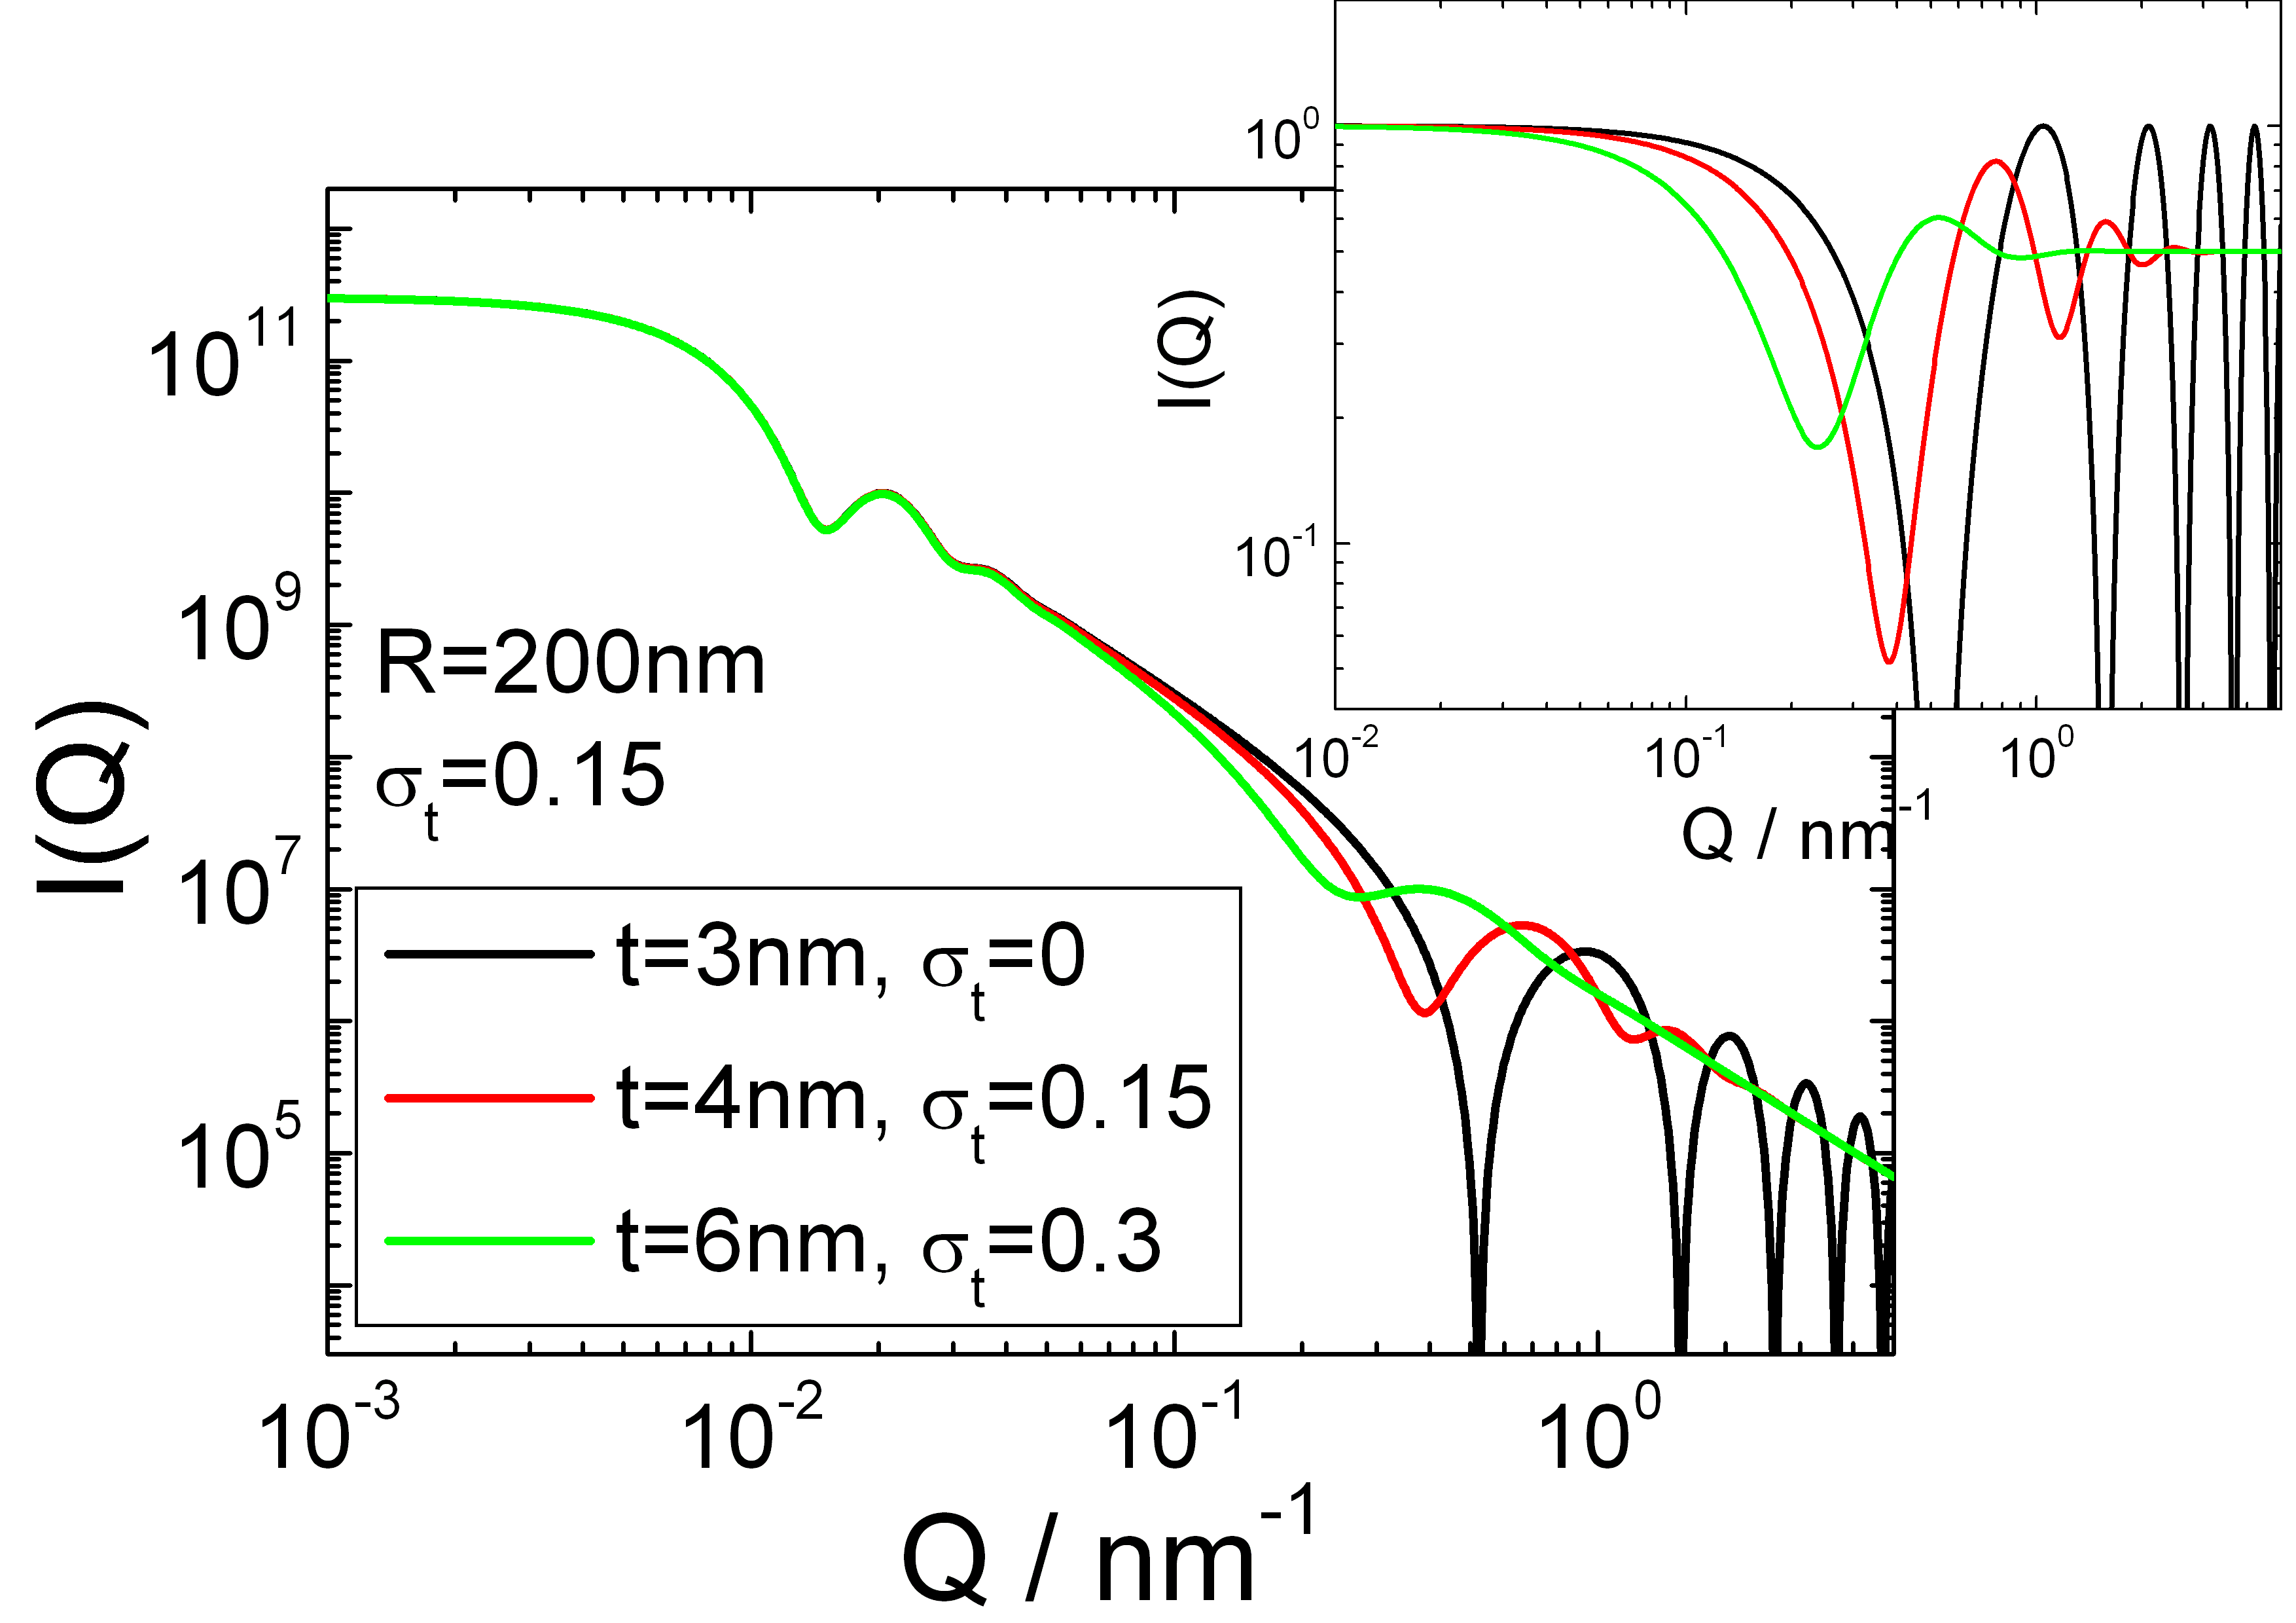
\includegraphics[width=0.8\textwidth,height=0.55\textwidth]{../images/form_factor/anisotropic/planar2thinIQ.png}
\end{center}
\caption{Scattering curve for the form factor "\texttt{Pcs:TwoInfinitelyThinLayers}" only (insert) and
in combination with a structure factor "\texttt{P'(Q): Thin Spherical Shell}".}
\label{fig_IQ:Pcs:TwoInfinitelyThinLayers}
\end{figure}


\clearpage
\subsubsection{Pcs(Q) for a layered centro symmetric cross-section structure} ~\\
\label{plugin:Pcs:LayeredCentroSymmetricCrossSectionStructure}

\begin{figure}[htb]
\begin{center}
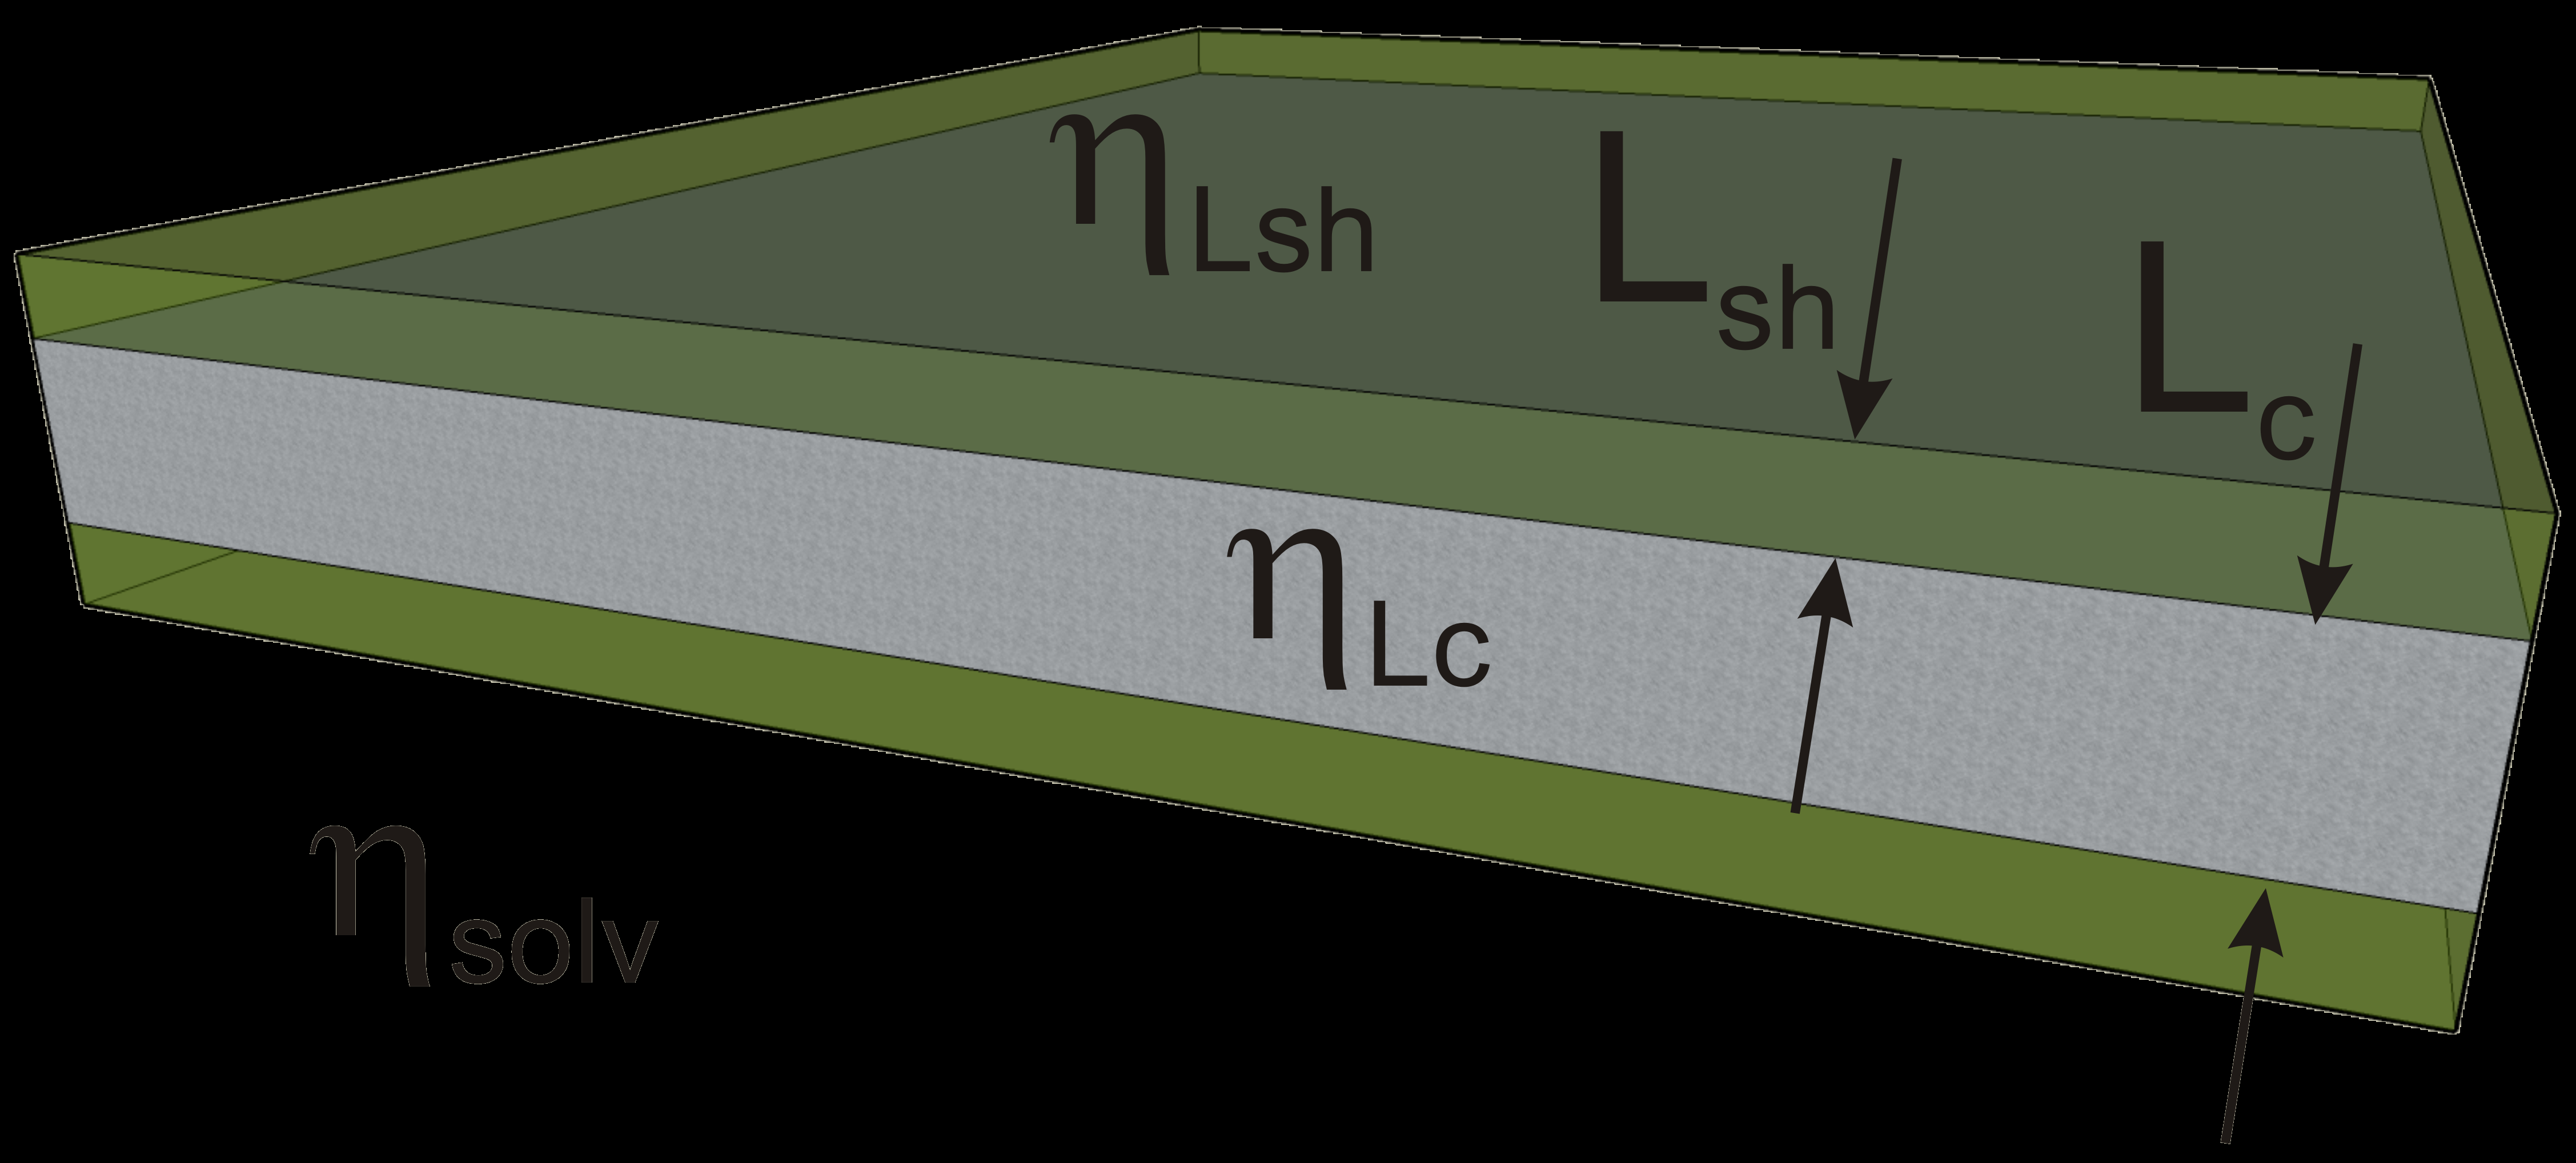
\includegraphics[width=0.8\textwidth,height=0.361\textwidth]{../images/form_factor/anisotropic/planar2centrosymm_txt.png}
\end{center}
\caption{Two layered centro symmetric structure with a core thickness of $L_\textrm{c}$ and an outer layer thickness
$L_{L_\textrm{sh}}$. The corresponding scattering length densities of the core, the shell layer and the solvent are
$L_{L_\textrm{c}}$, $L_{L_\textrm{sh}}$, and $L_{L_\textrm{solv}}$.}
\label{fig:Pcs:TwoInfinitelyThinLayers}
\end{figure}

This cross-section form factor describes the scattering of a layered centro symmetric cross-section structure.
Both the core thickness as well as the shell thickness can have a distribution described by a log-normal distribution as defined in eq.\ \ref{eq:LogNormal}.

\begin{multline}
P_\text{cs}(Q,\sigma_{L_\textrm{c}},L_\textrm{c},\sigma_{L_\textrm{sh}},L_\textrm{sh},\eta_{L_\textrm{c}},\eta_{L_\textrm{sh}},\eta_\textrm{sol}) = \\
\int_0^\infty \textrm{LogNorm}(v,1,\sigma_{L_\textrm{c}},1,L_\textrm{c})
\int_0^\infty \textrm{LogNorm}(u,1,\sigma_{L_\textrm{sh}},1,L_\textrm{sh}) \\
     \Bigg[ \frac{(\eta_{L_\textrm{sh}}-\eta_\textrm{solv})(v+2u) \sin\left(Q\frac{v+2u}{2}\right)}{Q\frac{v+2u}{2}}
          -\frac{(\eta_{L_\textrm{sh}}-\eta_{L_\textrm{c}})  v   \sin\left(Q \frac{v}{2}\right)}{Q \frac{v}{2}}
    \Bigg]^2 \,
\textrm{d}u \, \textrm{d}v
\end{multline}

\noindent
\textbf{Input parameters for \texttt{Pcs:LayeredCentroSymmetricXS}:}
\begin{description}
    \item[\texttt{L\_c}] most probable layer separation $L_\textrm{c}$
    \item[\texttt{sigm\_Lc}] width $\sigma_{L_\textrm{c}}$ of core thickness distribution (LogNorm)
    \item[\texttt{L\_sh}] most probable shell thickness $L_\textrm{sh}$
    \item[\texttt{sigm\_Lsh}] width $\sigma_{L_\textrm{c}}$ of shell thickness distribution (LogNorm)
    \item[\texttt{eta\_Lc}] scattering length density of core layer $\eta_{L_\textrm{c}}$
    \item[\texttt{eta\_Lsh}] scattering length density of shell layer $\eta_{L_\textrm{sh}}$
    \item[\texttt{eta\_solv}] scattering length density of solvent $\eta_{solv}$
\end{description}

\noindent
\textbf{Note}
\begin{itemize}
  \item This form factor is supposed to be combined with a shape factor for
local planar objects which are implemented as structure  plugins
under "\texttt{[by plugin|anisotropic obj.|P'(Q): local planar
obj.]}".
\item As the form factor already have the width distribution included one normally uses in \SASfit as a size distribution
the \texttt{Delta}-distribution.
\end{itemize}

\begin{figure}[htb]
\begin{center}
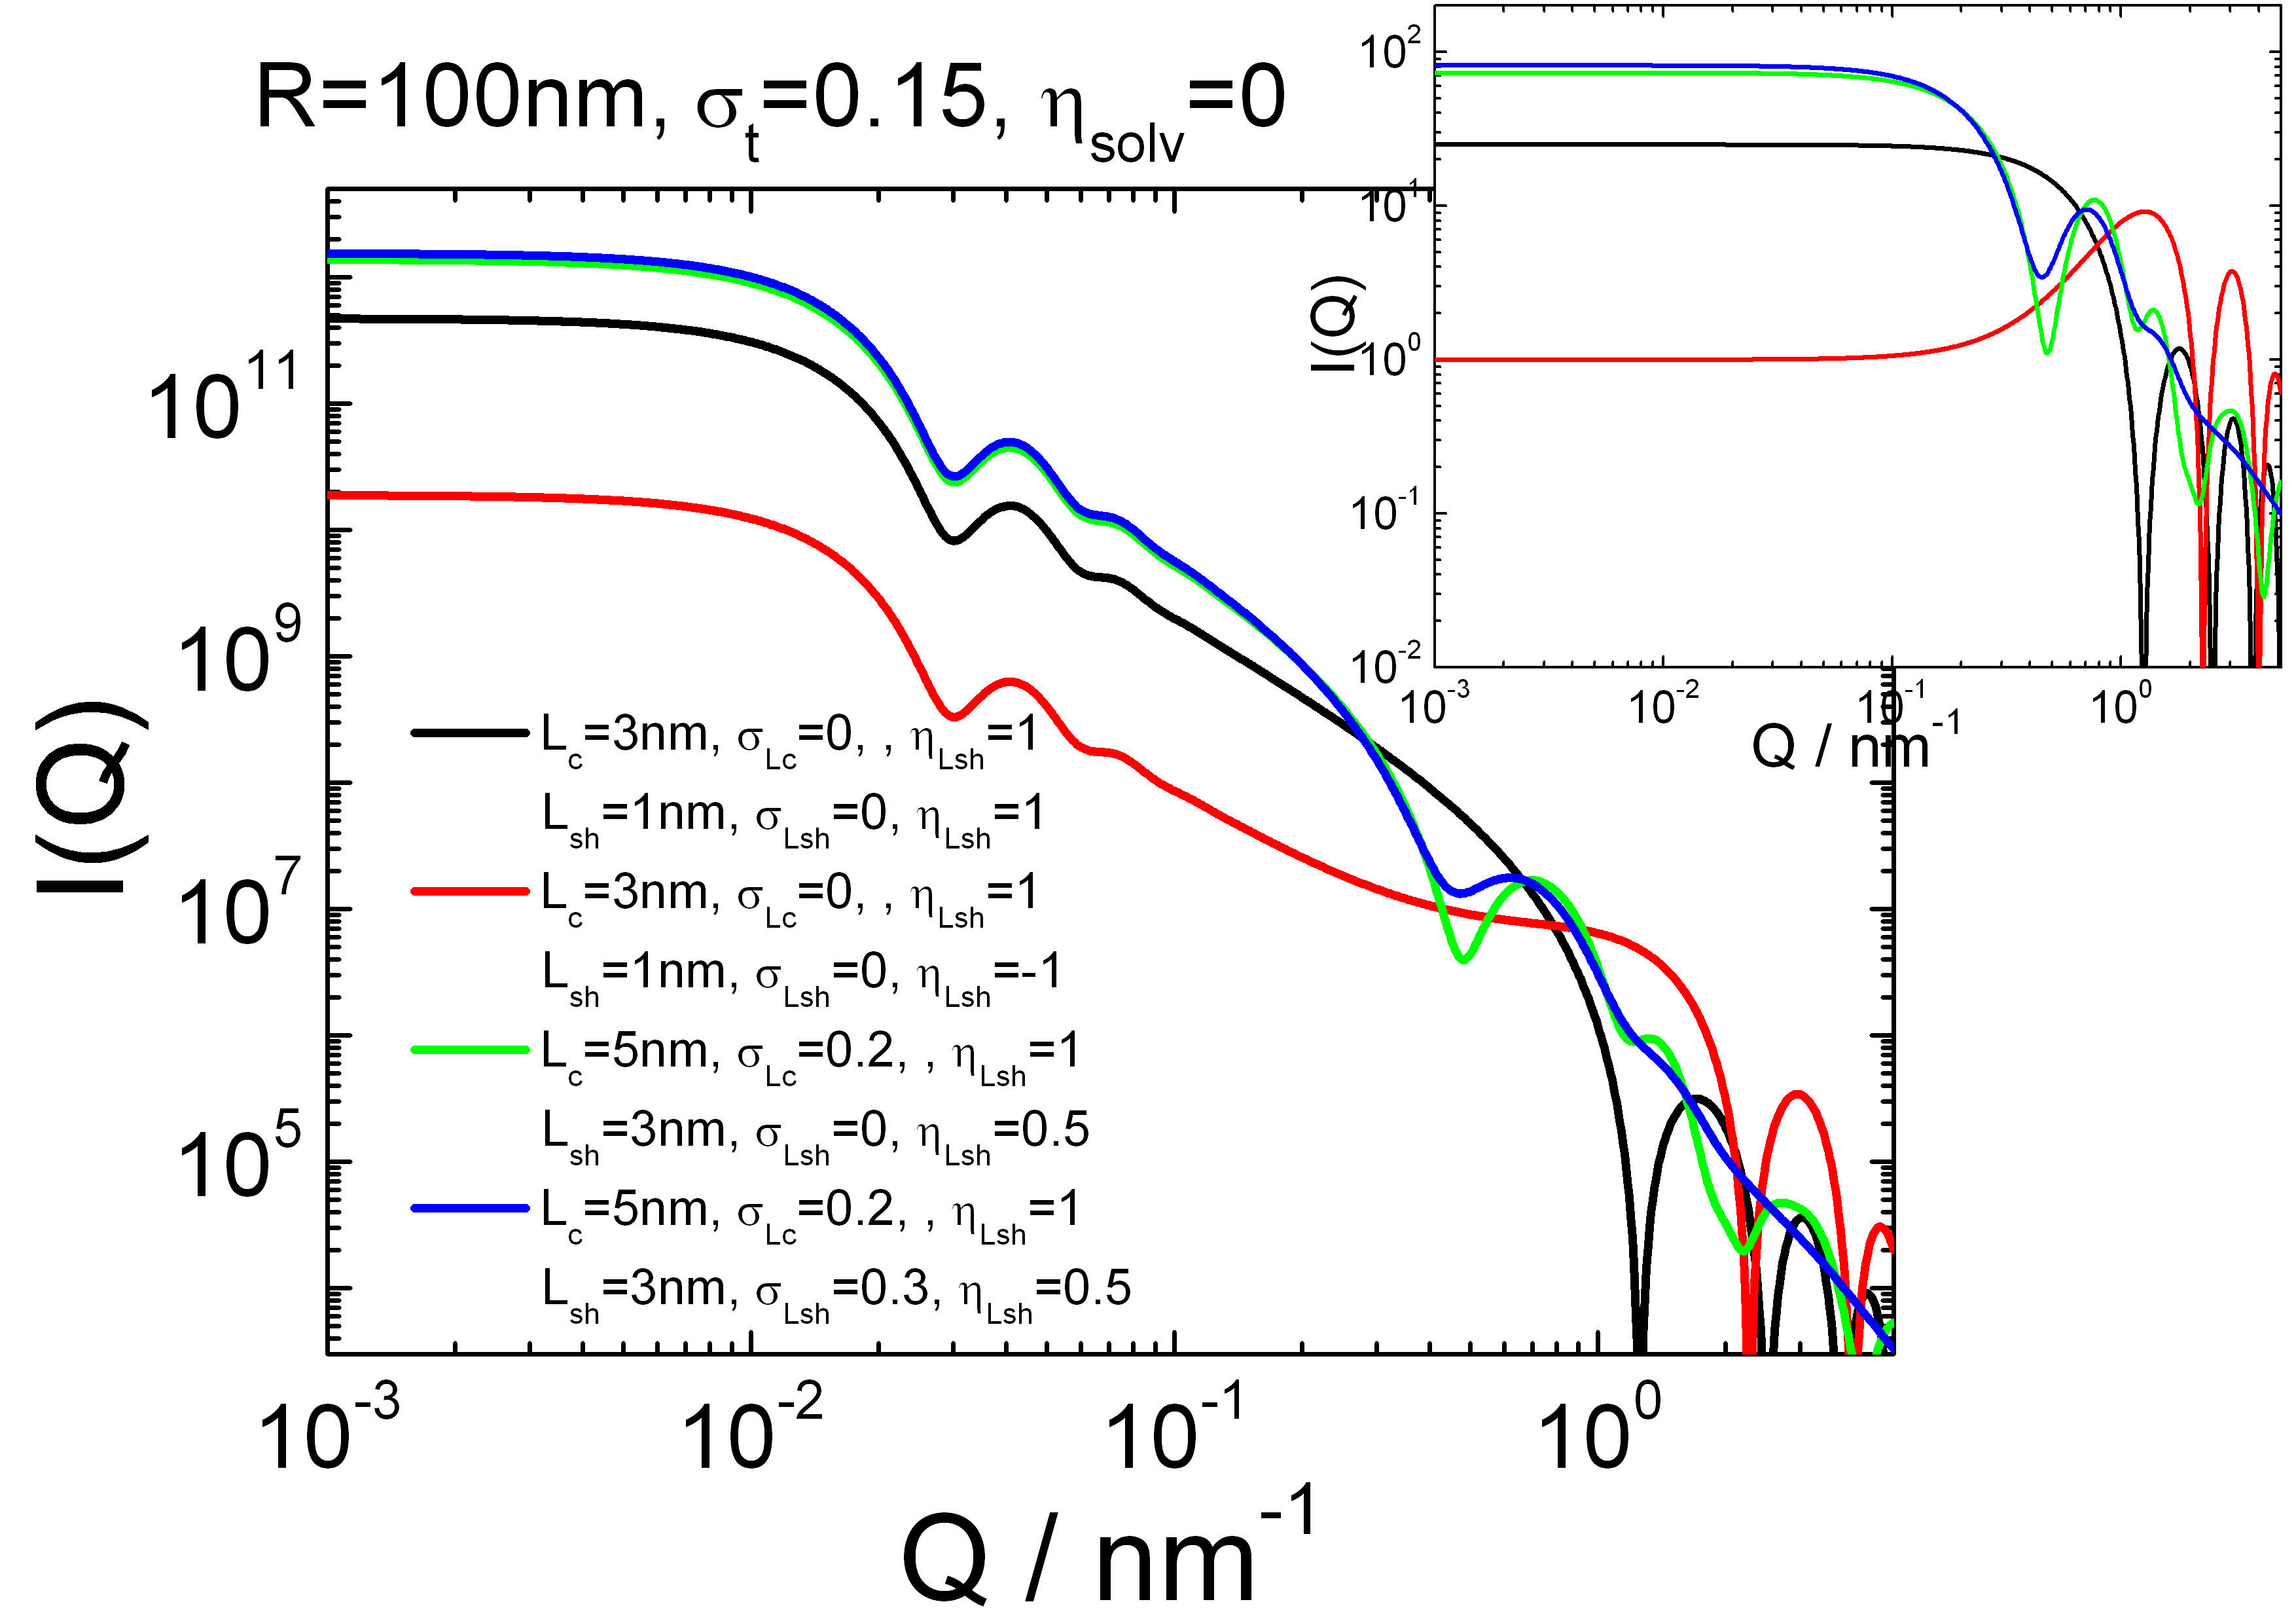
\includegraphics[width=0.8\textwidth,height=0.55\textwidth]{../images/form_factor/anisotropic/Pcs_planar2centrosymmIQ.png}
\end{center}
\caption{Scattering curve for the form factor "\texttt{Pcs:LayeredCentroSymmetricXS}" only (insert) and
in combination with a structure factor "\texttt{P'(Q): Thin Spherical Shell}".}
\label{fig:Pcs_planar2centrosymmIQ}
\end{figure}

\clearpage

\subsubsection{Pcs(Q) for a bilayer with a Gaussian electron density profile \cite{Pabst2000,Pabst2003}} ~\\
\label{plugin:Pcs:GaussianProfile}

\begin{figure}[htb]
\begin{center}
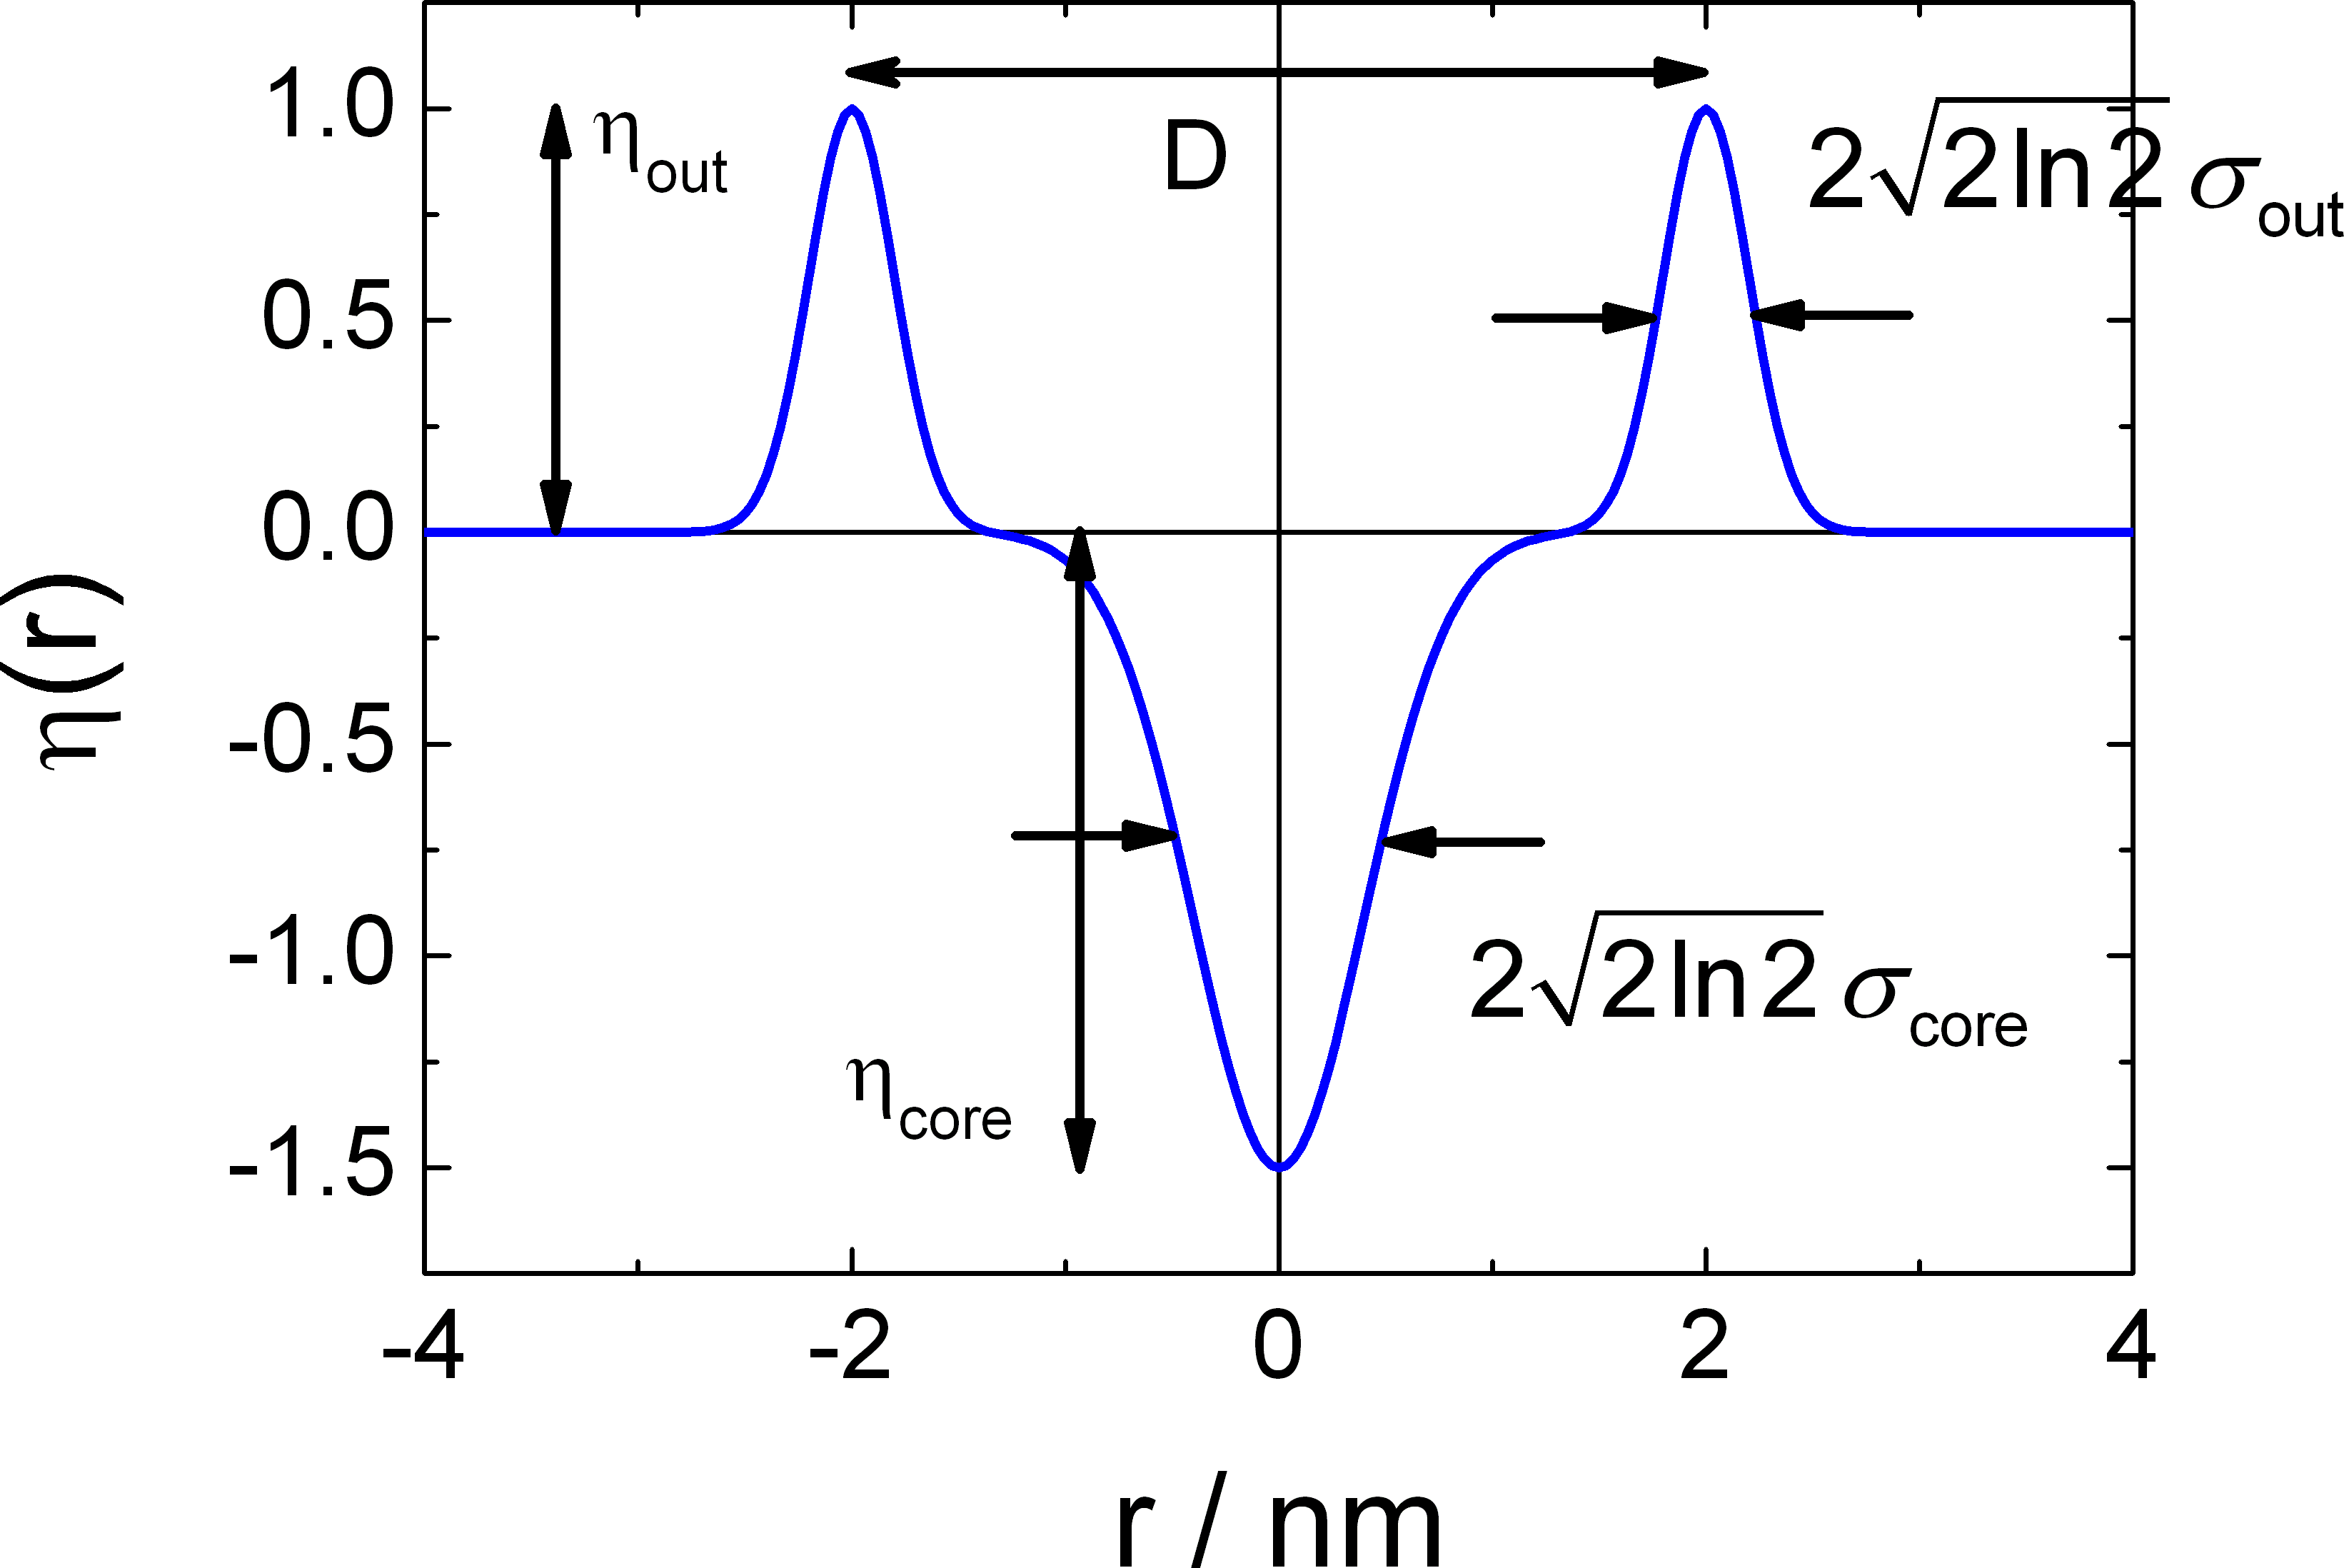
\includegraphics[width=0.8\textwidth,height=0.55\textwidth]{../images/form_factor/anisotropic/BiLayerGauss_Profile.png}
\end{center}
\caption{
The plot shows a model for the Gaussian description of the bilayer electron density profile according to
eq.\ \ref{eq:BiLayerGaussianProfile}.
The origin of the profile is set to the bilayer centre. The model encountering a single Gaussian for the head
group at $\pm t/2$. $\eta_\textrm{out}$ is the amplitude of the headgroup Gaussian and $\eta_\textrm{core}$ that of
the hydrocarbon chains with respect to the average electron density of water. The FWHM of the Gaussian profiles are
$2\sqrt{2\ln 2}\sigma_\textrm{out}$ and $2\sqrt{2\ln 2}\sigma_\textrm{core}$.}
\label{fig:bilayerprofile}
\end{figure}

This model for a bilayer is using a real-space representation of the electron density profile
using a Gaussian description \cite{Pabst2000,Pabst2003}. In comparison to other models it
is simpler and requiring the adjustment of only four parameters. The electron density profile
(Fig.\ \ref{fig:bilayerprofile}) is described by
\begin{align}
\begin{split}
\eta(r) &=  \eta_\textrm{out} \left[ \exp\left(-\frac{\left(r-\frac{t}{2}\right)^2}{2\sigma_\textrm{out}^2}\right) +
   \exp\left(-\frac{\left(r+\frac{t}{2}\right)^2}{2\sigma_\textrm{out}^2}\right) \right] \\
          &+ \eta_\textrm{core} \exp\left(-\frac{r^2}{2\sigma_\textrm{core}^2}\right)
          \label{eq:BiLayerGaussianProfile}
\end{split}
\end{align}
The scattering intensity of this cross section profile of a planar object can be calculated by eq.\ \ref{Pcs:planar}
and computes as
\begin{align}
   F_\text{out}\left(Q,D,\sigma_\textrm{out},\eta_\textrm{out}\right)  &= \sqrt{2\pi}\sigma_\textrm{out}  \eta_\textrm{out}  \exp\left(-\frac{1}{2}\left(Q\sigma_\textrm{out} \right)^2\right) \cos\left(Q\frac{t}{2}\right) \\
   F_\text{core}\left(Q,\sigma_\textrm{core},\eta_\textrm{core}\right) &= \sqrt{2\pi}\sigma_\textrm{core} \eta_\textrm{core} \exp\left(-\frac{1}{2}\left(Q\sigma_\textrm{core}\right)^2\right)
\end{align}
so that
\begin{align}
  P_\text{cs}\left(Q\right)   &=\left[F_\text{core}\left(Q,\sigma_\textrm{core}, \eta_\textrm{core}\right)
                                   +2 F_\text{out} \left(Q,D,\sigma_\textrm{out},\eta_\textrm{out} \right)\right]^2
  \label{eq:PcsBilayer}
\end{align}

\noindent
\textbf{Input parameters for \texttt{Pcs:BilayerGauss}:}
\begin{description}
    \item[\texttt{sigma\_core}] width $\sigma_\mathrm{out}$ of the central Gaussian profile
    \item[\texttt{eta\_core}] scattering length density contrast of the central Gaussian profile
    \item[\texttt{sigma\_out}] width $\sigma_\mathrm{out}$ of the two outer Gaussian profiles
    \item[\texttt{eta\_out}] scattering length density contrast of the two outer Gaussian profiles
    \item[\texttt{t}] distance between the centers of the outer Gaussian profiles
\end{description}

\noindent
\textbf{Note}
\begin{itemize}
  \item This form factor is supposed to be combined with a shape factor for
local planar objects which are implemented as structure  plugins
under "\texttt{[by plugin|anisotropic obj.|P'(Q): local planar
obj.]}".
\end{itemize}

\begin{figure}[htb]
\begin{center}
\subfigure[Plot of the cross section form factor $P_\text{cs}$ in combination with a structure factor "\texttt{P'(Q): Thin Disc}"
as the shape factor $P'(Q)$.]{
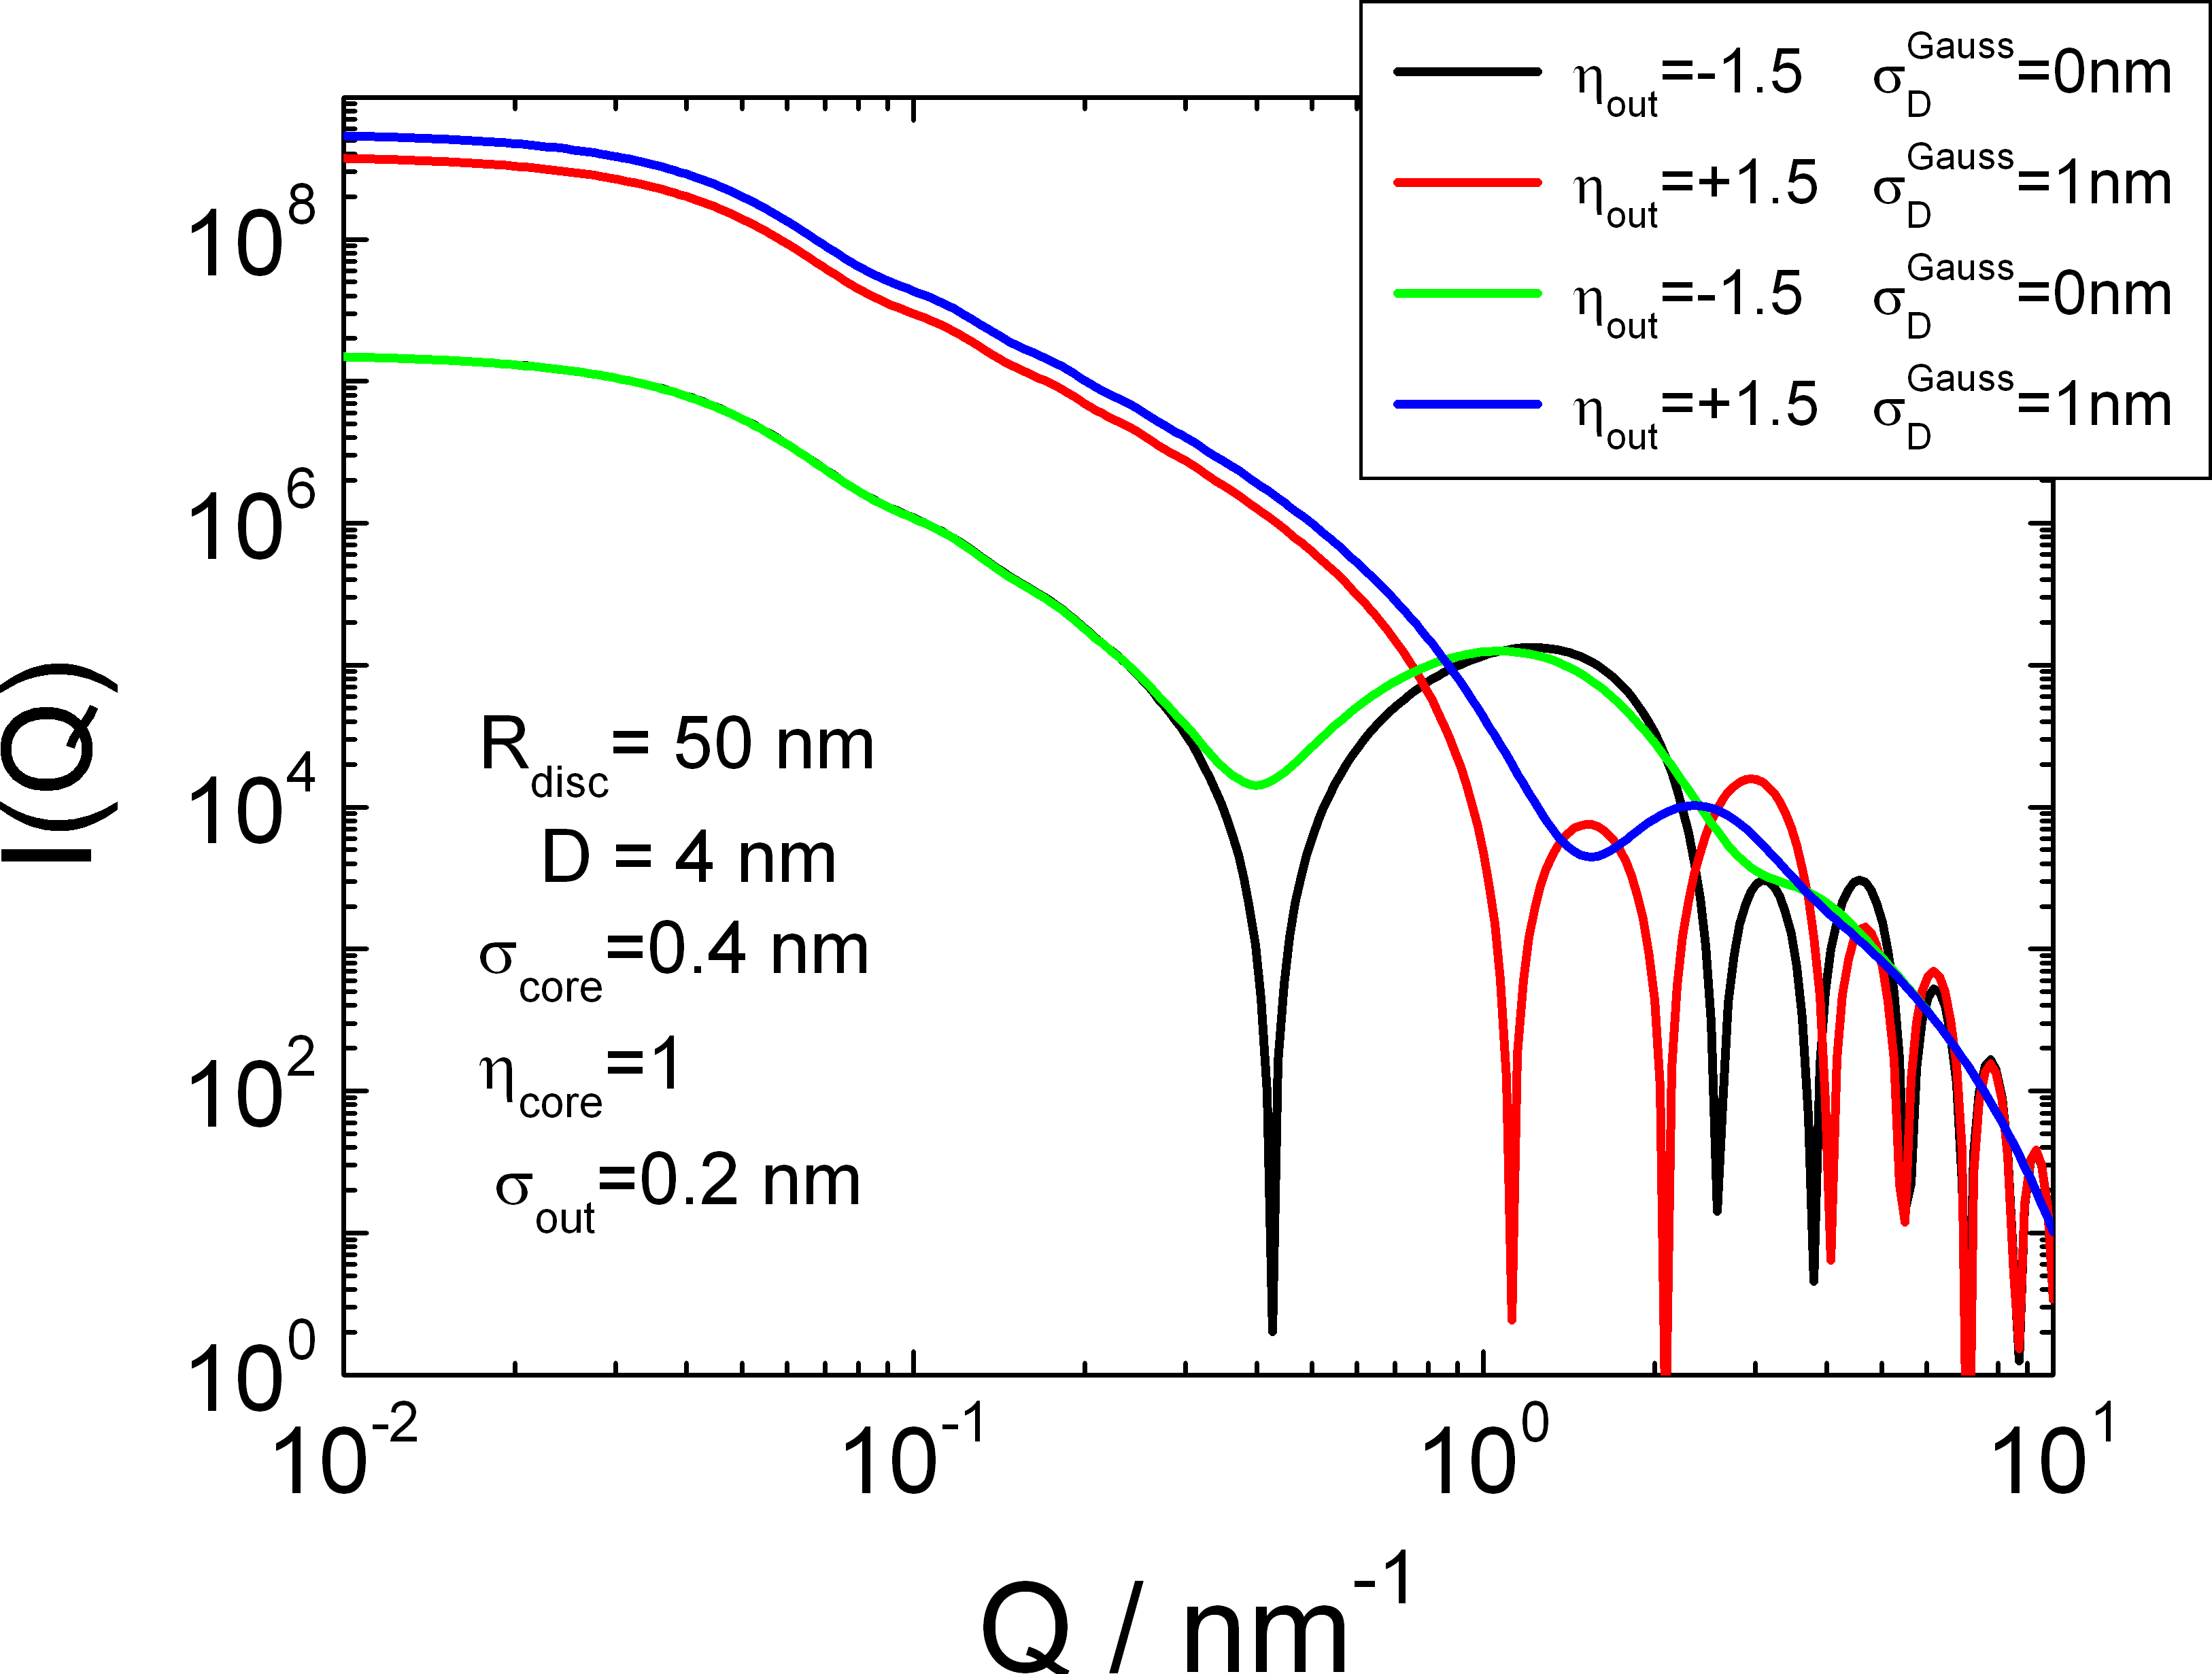
\includegraphics[width=0.48\textwidth,height=0.35\textwidth]{../images/form_factor/anisotropic/BiLayerGauss_IQa.png}}
\hfill
\subfigure[Plot of the cross section form factor $P_\text{cs}$ only according to eq.\ \ref{eq:PcsBilayer}.
The parameters for the profile are the same than in Fig.\ \ref{fig:BiLayerGaussianProfileIQ}a]{
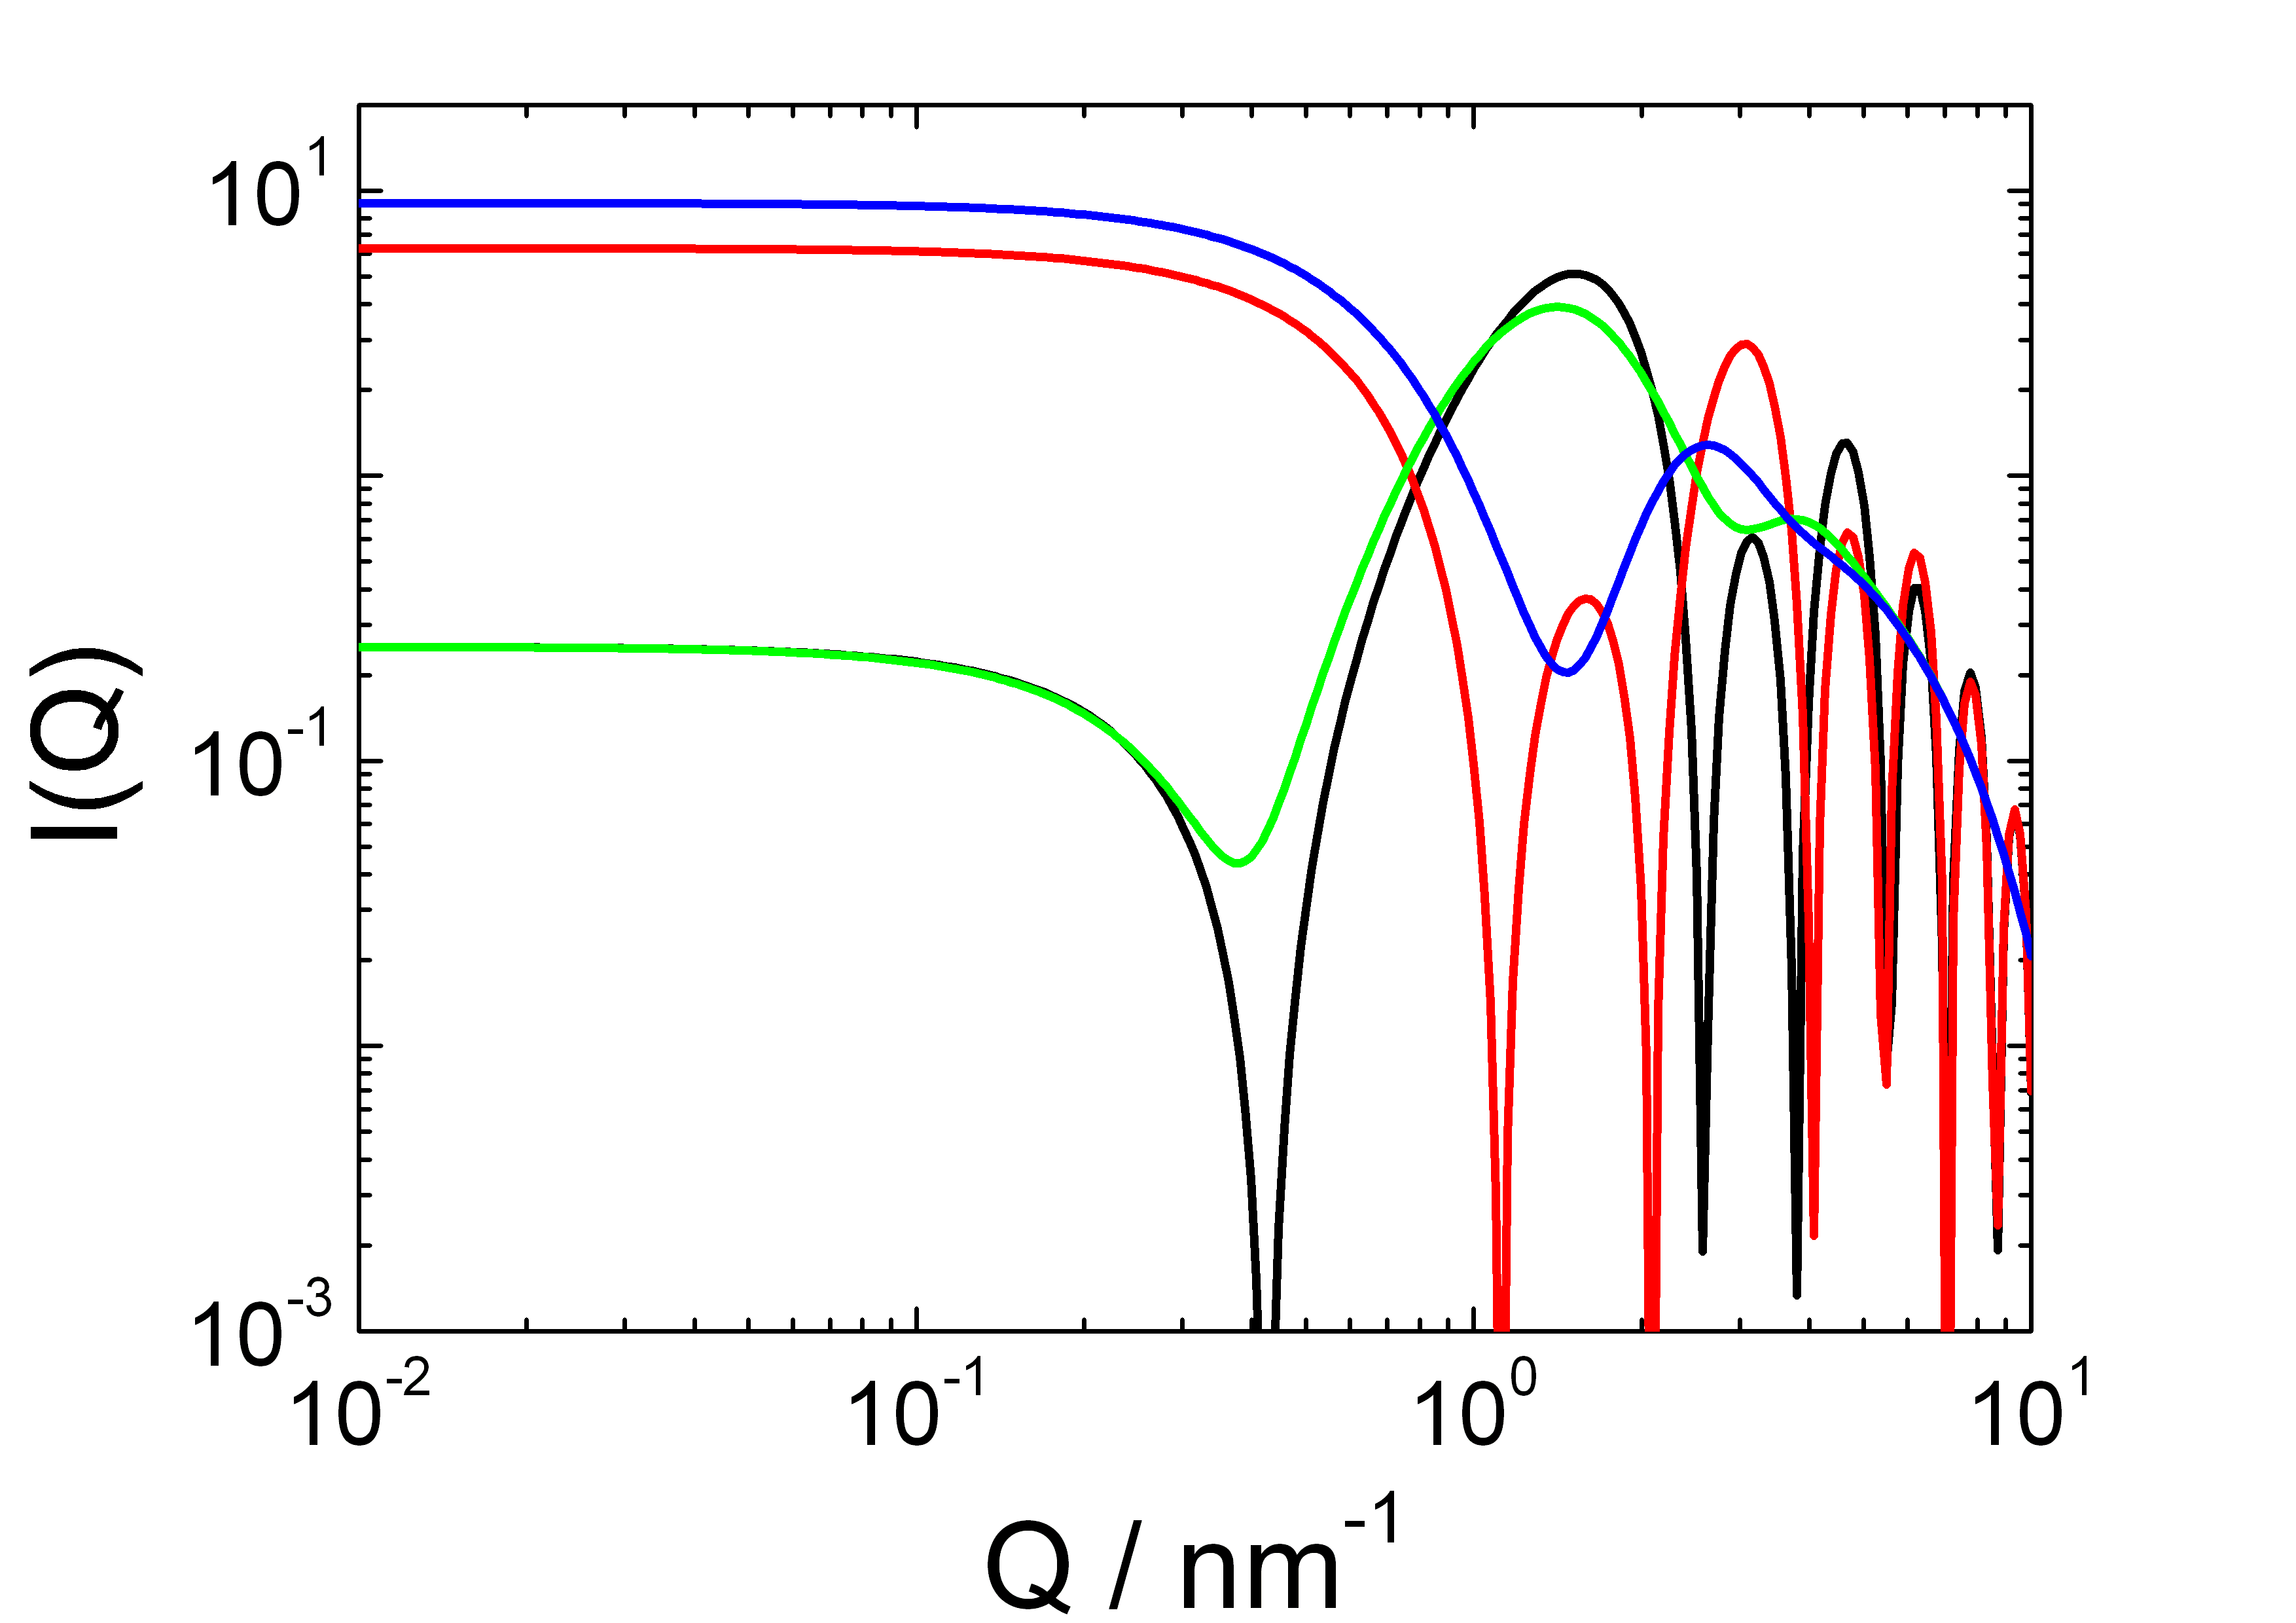
\includegraphics[width=0.48\textwidth,height=0.35\textwidth]{../images/form_factor/anisotropic/BiLayerGauss_IQb.png}}
\end{center}
\caption{Scattering curve for the cross-section form factor "\texttt{Pcs:BilayerGaussian}". For some of the curves a distance distribution of
the heads groups are assumed being Gaussian (see eq.\ \ref{eq:GaussDistribution}), i.e. calculating
$\int_0^\infty \mathrm{Gauss}(D,1,\sigma_D^\textrm{Gauss},D_0) P_\text{cs}\left(Q,D\right)\, \mathrm{d}D$.}
\label{fig:BiLayerGaussianProfileIQ}
\end{figure}


%
%\clearpage
%\subsubsection{Pcs(Q) for local planar objects with Gaussian chains attached to the  surface} ~\\
%\label{plugin:Pcs:GaussianChains}
%
%\begin{figure}[htb]
%\begin{center}
%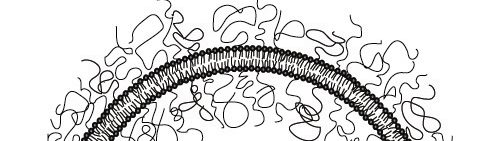
\includegraphics[width=0.962\textwidth,height=0.282\textwidth]{../images/form_factor/anisotropic/Plate+Chains(RW).png}
%\end{center}
%\caption{Sketch of a lipid bilayer with PEG molecules attached to them, which would be an example for local planar
%and objects with homogeneous core and Gaussian chains attached to the surface.}
%\label{fig:Plate+Chains(RW)}
%\end{figure}
%
%This cross-section form factor belongs to a whole class of form factors developed from
%Pedersen, Gerstenberg, and Svaneborg
%\cite{PedersenJApplCryst2000,PedersenGerstenberg96,SvaneborgPedersen2002,Richter1997}
%for self assembled block copolymers forming micelles of different shapes.
%They have assumed that one unit is forming the core of the
%micelles and the other the corona. The core is assumed to have a
%homogeneous scattering length density, but may contain some amount
%of solvent whereas the soluble blocks form a diffuse corona surrounding the core.
%
%The cross-section form factor of a micelle contains four different terms \cite{Pedersen2002}
%\begin{align}
%\begin{split}
%P_\text{cs}(Q)
% &=  \Bigg( r_\textrm{core}^2\,\left(\frac{\sin(QL/2)}{QL/2}\right)^2 + r_\textrm{brush} N_\text{agg} P_\text{brush}(Q)  \\
% & + N_\text{agg}(N_\text{agg}-1)r_\text{brush}^2\,S_\textrm{bb}(Q) + 2N_\text{agg} r_\text{core}r_\text{brush}\,S_\text{bc}(Q)\Bigg)
%\end{split}
%\end{align}
%where $N_\text{agg}$ is the total aggregation number of polymers on the surface, and
%$r_\text{brush}=V_\text{brush}(\eta_\text{brush}-\eta_\text{solv})$
%the excess scattering length of a single polymer chain in the corona
%and $r_\text{core}=V_\text{core}(\eta_\text{core}-\eta_\text{solv})$
%the total  excess scattering length of the core, respectively.
%$V_\text{brush}$ is the volume of a a single polymer chain in the corona
%and $V_\text{core}$ the total volume of the core. $\eta_\text{brush}$ and $\eta_\text{core}$ are the corresponding
%scattering length densities and $\eta_\text{solv}$ is the scattering length
%density of the surrounding solvent.
%
%The functions $P_\text{core}(Q)$, $P_\text{brush}(Q)$,
%$S_\text{bc}(Q)$, and $S_\text{bb}(Q)$ are all 1 for $q=0$.
%They are defined as
%
%\noindent
%\textbf{Input parameters for \texttt{Pcs:Plate+Chains(RW)}:}
%\begin{description}
%    \item[\texttt{L\_core}] thickness of the core of the planar layer $L_\textrm{core}$
%    \item[\texttt{n\_agg}] specific aggregation number $n_\textrm{agg}$ in units of number of chains per surface area
%    \item[\texttt{V\_brush}]  molecular volume of single chain in corona $V_\textrm{brush}$ in nm$^3$ for $Q$ in nm$^{-1}$
%                              or in \AA$^3$ for $Q$ in \AA$^{-1}$
%    \item[\texttt{eta\_core}] scattering length density of the core $\eta_\textrm{core}$
%    \item[\texttt{eta\_brush}] scattering length density of a Gaussian chain in corona $\eta_\textrm{brush}$
%    \item[\texttt{eta\_solv}] scattering length density of solvent $\eta_\textrm{solv}$
%    \item[\texttt{xsolv\_core}] amount of solvent in core $X_\textrm{xsolc,core}$
%    \item[\texttt{Rg}] gyration radius $R_G$ of polymer chains in the corona
%    \item[\texttt{d}] Value $d$ should be around 1.
%                      Non-penetration of the chains into the core is mimicked by $d\simeq 1$ for $L_\textrm{core} \gg R_G$
%\end{description}
%
%\noindent
%\textbf{Note}
%\begin{itemize}
%  \item This form factor is supposed to be combined with a shape factor for
%local planar objects which are implemented as structure  plugins
%under "\texttt{by plugin|anisotropic obj.|P'(Q): local planar
%obj.}".
%\end{itemize}
%
%\begin{figure}[htb]
%\begin{center}
%\subfigure[Plot of the cross section form factor $P_\text{cs}$ only according to eq.\ \ref{eq:PcsBilayer}.]{
%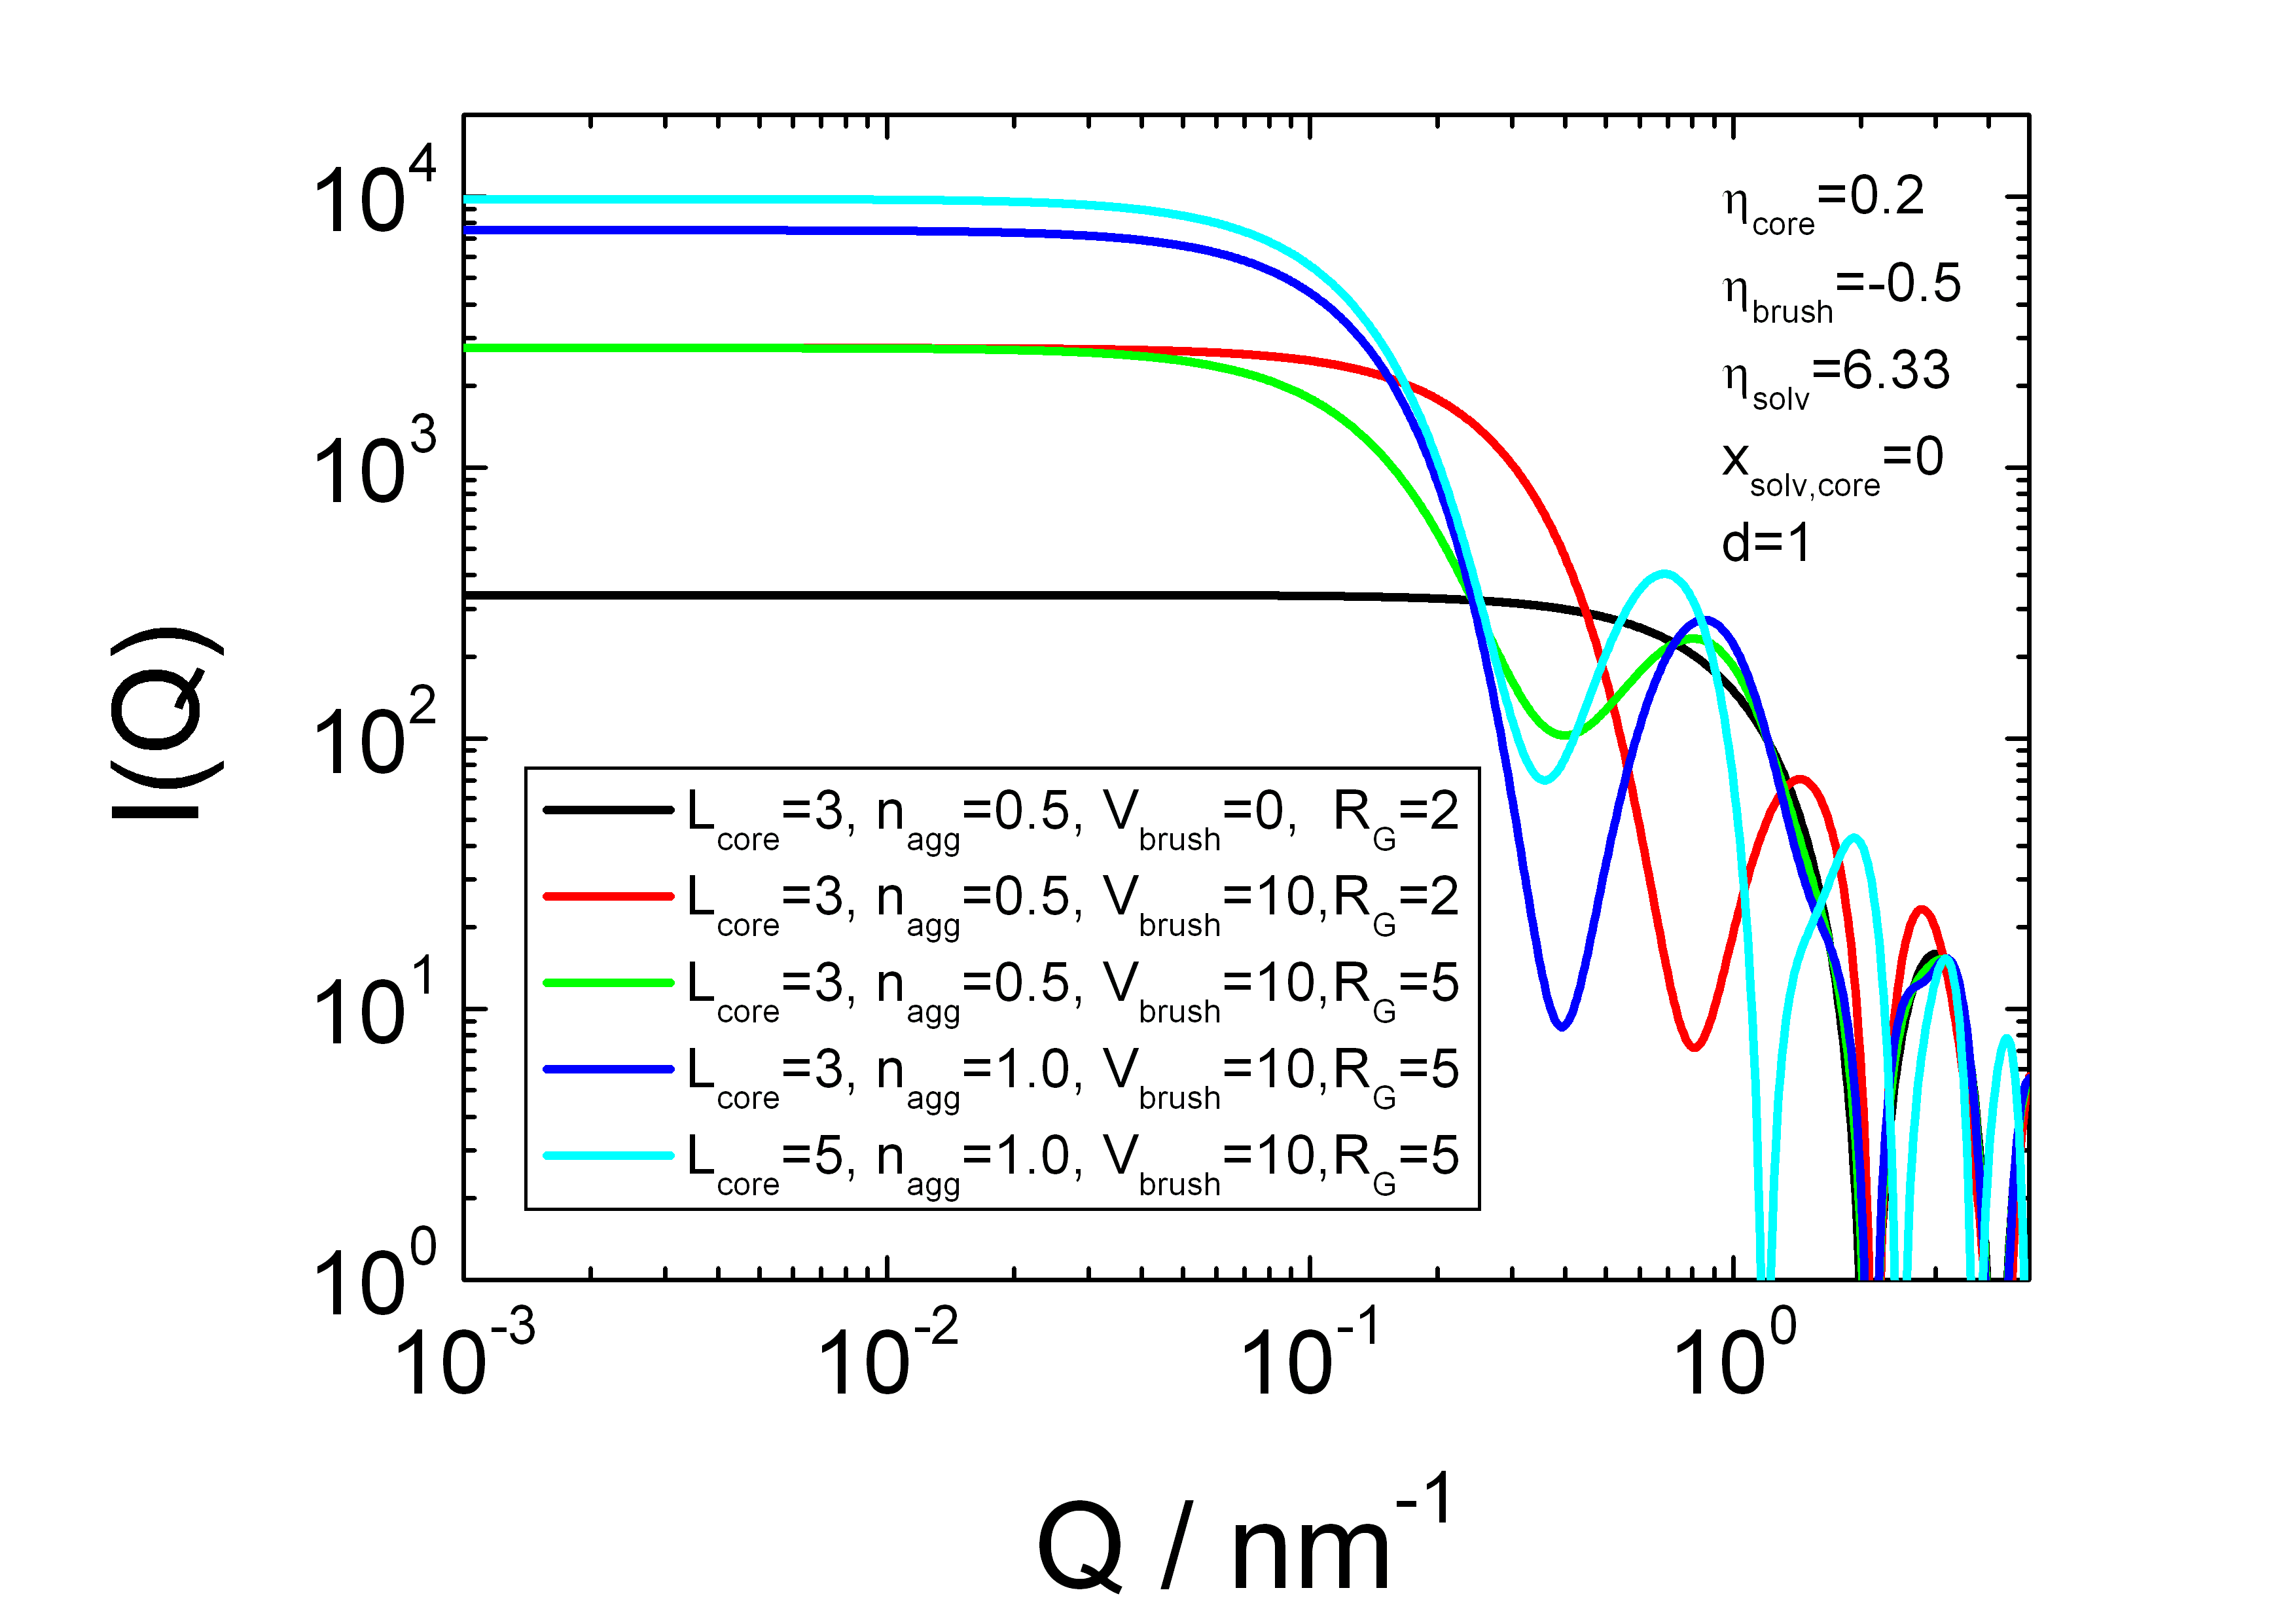
\includegraphics[width=0.48\textwidth,height=0.35\textwidth]{../images/form_factor/anisotropic/Pcs_Plate_Chains_RW_IQa.png}}
%\hfill
%\subfigure[Plot of the cross section form factor $P_\text{cs}$ in combination with a structure factor "\texttt{P'(Q): Thin Spherical Shell}"
%as the shape factor $P'(Q)$. The parameters for the profile are the same than in Fig.\ \ref{fig:Pcs_Plate_Chains_RW_IQ}a]{
%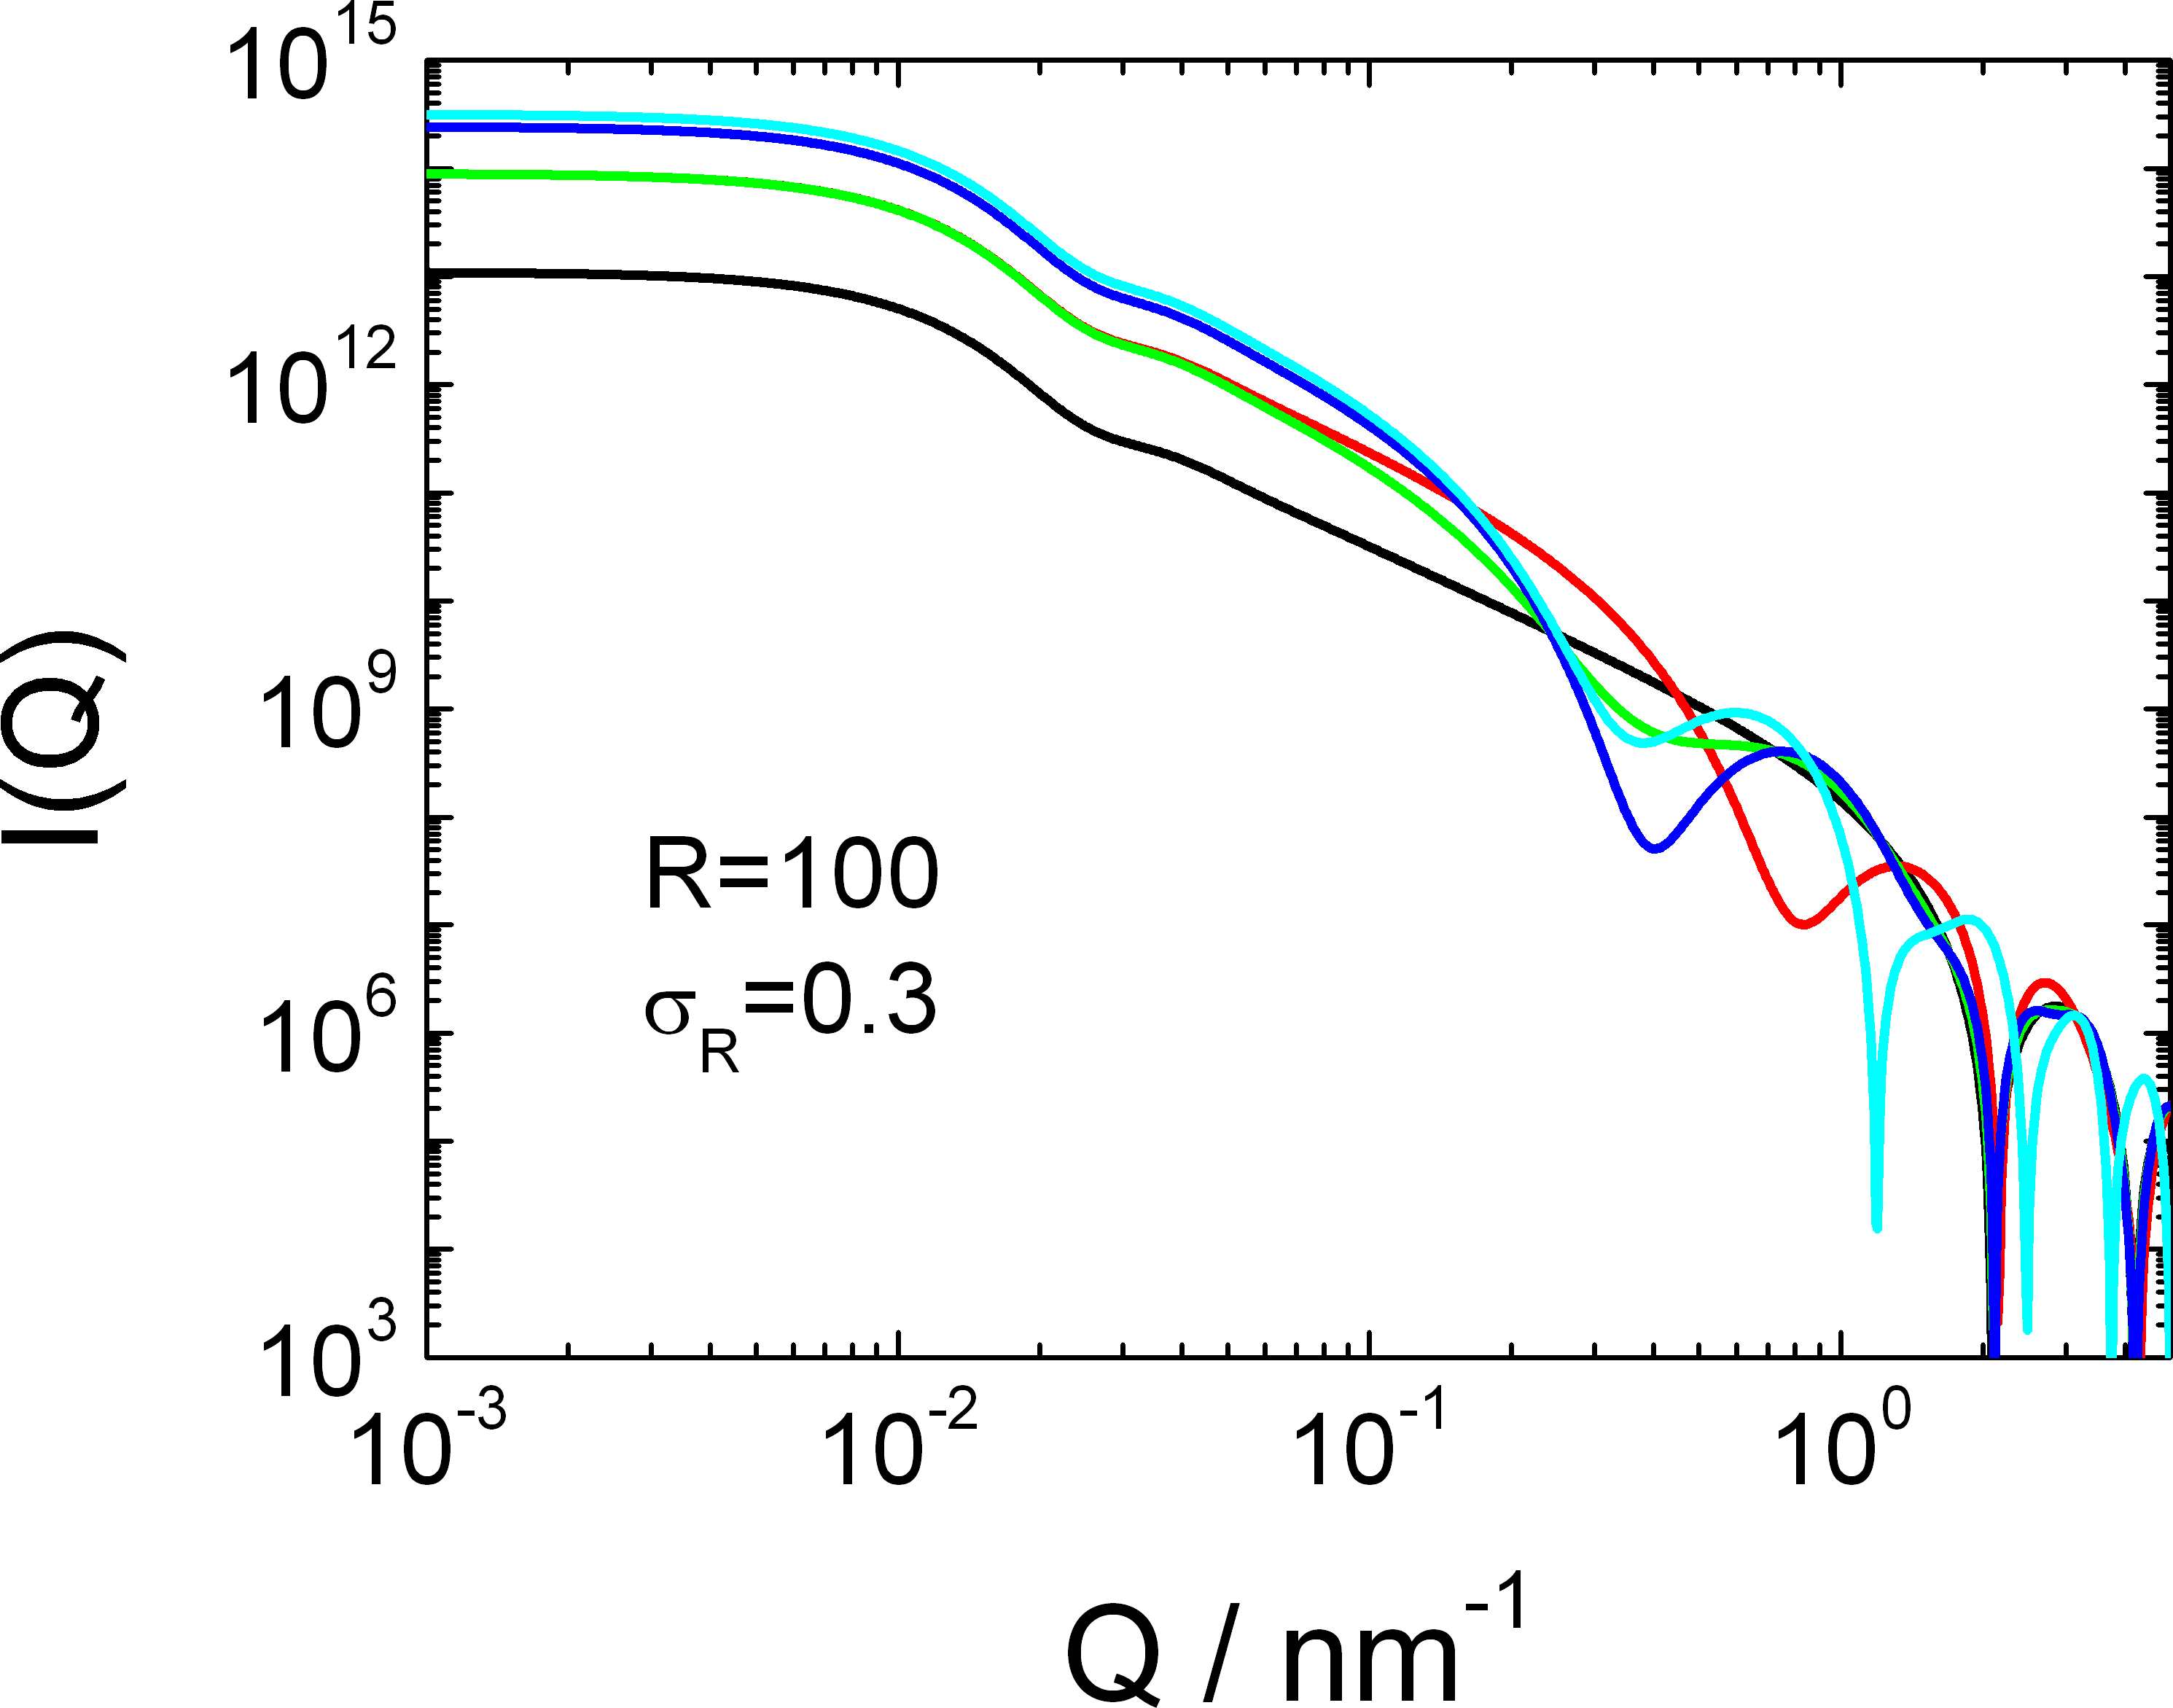
\includegraphics[width=0.48\textwidth,height=0.35\textwidth]{../images/form_factor/anisotropic/Pcs_Plate_Chains_RW_IQb.png}}
%\end{center}
%\caption{Scattering curves for the cross-section form factor "\texttt{Pcs:Plate+Chains(RW)}".}
%\label{fig:Pcs_Plate_Chains_RW_IQ}
%\end{figure}

\clearpage
\subsection{Pcs(Q) for cylindrical obj.} ~\\
\label{plugin:Pcs4cylindrical}

The cross-section form factors with cylindrical geometry are valid
when the cross-section dimension is much smaller than the segment length
or Kuhn length of the local cylindrical structure.

\begin{figure}[htb]
  % Requires \usepackage{graphicx}
  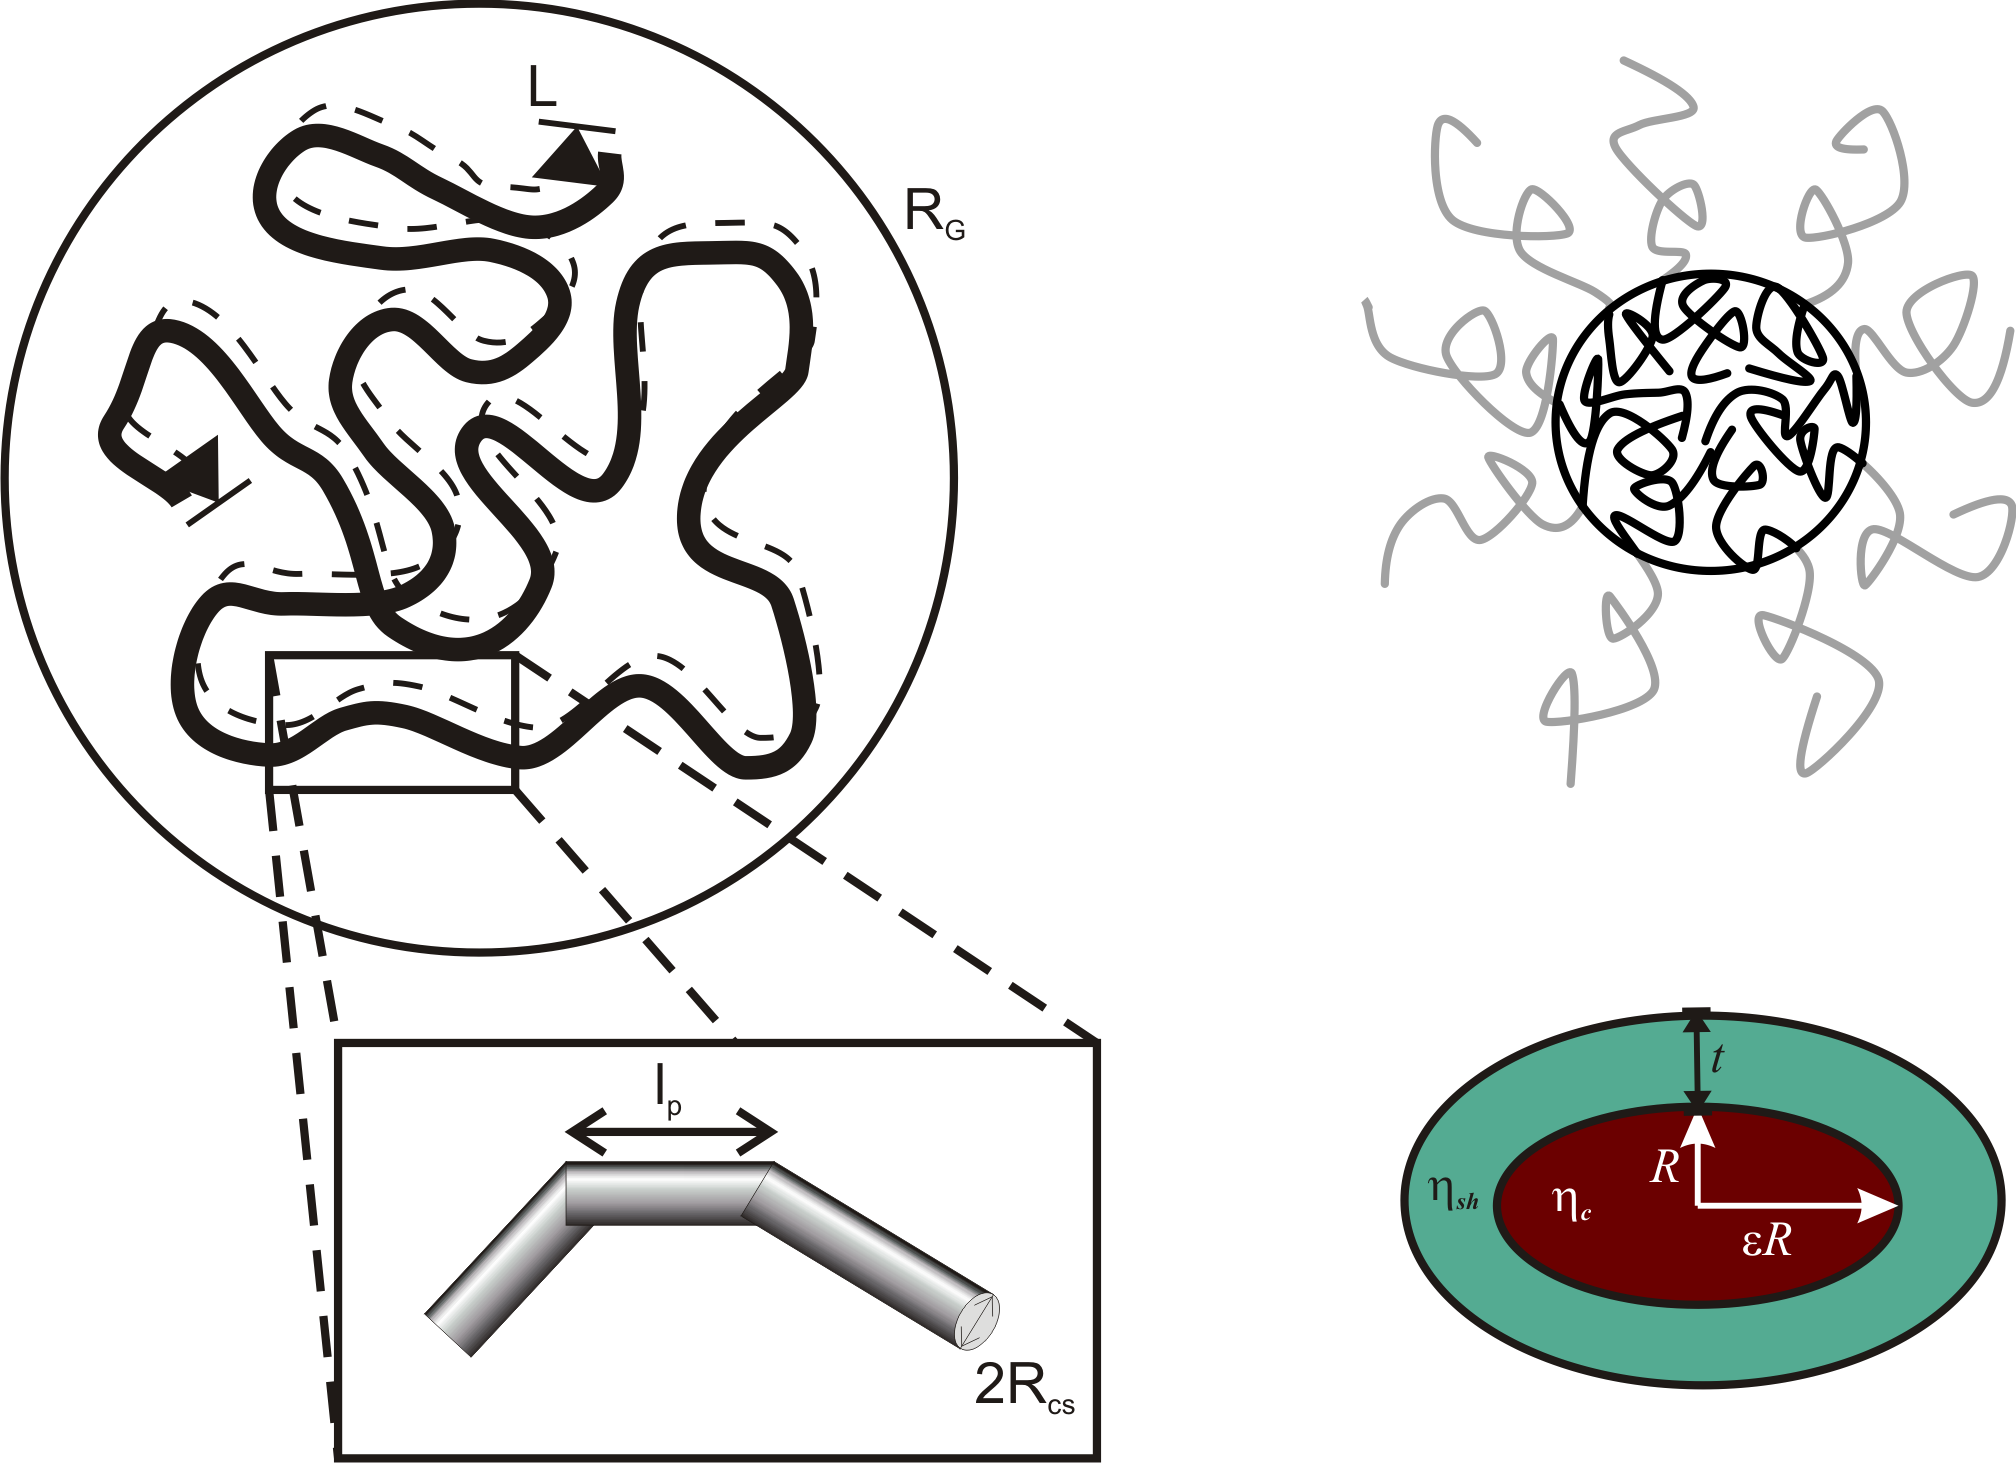
\includegraphics[width=0.85\textwidth]{../images/form_factor/anisotropic/SketchdiffXSWorm.png}\\
  \caption{Sketch of wormlike structures which represent local cylindrical structures. The cross-section $2R_\text{cs}$
  is much smaller than the Kuhn length $l_p$, which is a typical length scale where a freely jointed chain can randomly orient
  in any direction without the influence of any forces, independent of the directions taken by other segments.
  For the cross-section term several profiles have been implemented, like homogeneous round profile or elliptical shell profile}\label{fig:WormSketchdiffXS}
\end{figure}


\clearpage
\subsubsection{Pcs(Q) for homogeneous cross-section of a cylinder} ~\\
\label{plugin:Pcs:homogeneousXS_cyl}


This cross-section form factor describes the scattering of circular and homogeneous cross section.
The cross-section radius $R$ can have a distribution described by a log-normal distribution according
to eq.\ \ref{eq:LogNormal}.

\begin{align}
P_\text{cs}(Q,\sigma_{R},R) = \int_0^\infty \textrm{LogNorm}(x,1,\sigma_{R},1,R) \left( \left(\eta_\textrm{core}-\eta_\textrm{solv}\right) \pi x^2 \frac{2 \mathrm{J}_1(Qx)}{Qx} \right)^2 \, \textrm{d}x
\end{align}

\noindent
\textbf{Input parameters for \texttt{Pcs:homogeneousCyl}:}
\begin{description}
    \item[\texttt{R}] most probable radius $R$
    \item[\texttt{sigm\_R}] width $\sigma_R$ of radius distribution (LogNorm)
    \item[\texttt{dummy}] not used
    \item[\texttt{dummy}] not used
    \item[\texttt{dummy}] not used
    \item[\texttt{dummy}] not used
    \item[\texttt{dummy}] not used
    \item[\texttt{eta\_core}] scattering length density of the core $\eta_\textrm{core}$
    \item[\texttt{dummy}] not used
    \item[\texttt{eta\_solv}] scattering length density of the solvent $\eta_\textrm{solv}$
\end{description}

\noindent
\textbf{Note}
\begin{itemize}
  \item This form factor is supposed to be combined with a shape factor for
local cylindrical objects which are implemented as structure  plugins
under "\texttt{[by plugin|anisotropic obj.|P'(Q): local cylindrical obj.]}".
\item As the form factor already have the width distribution included one normally uses in \SASfit as a size distribution
the \texttt{Delta}-distribution.
\end{itemize}

\begin{figure}[htb]
\begin{center}
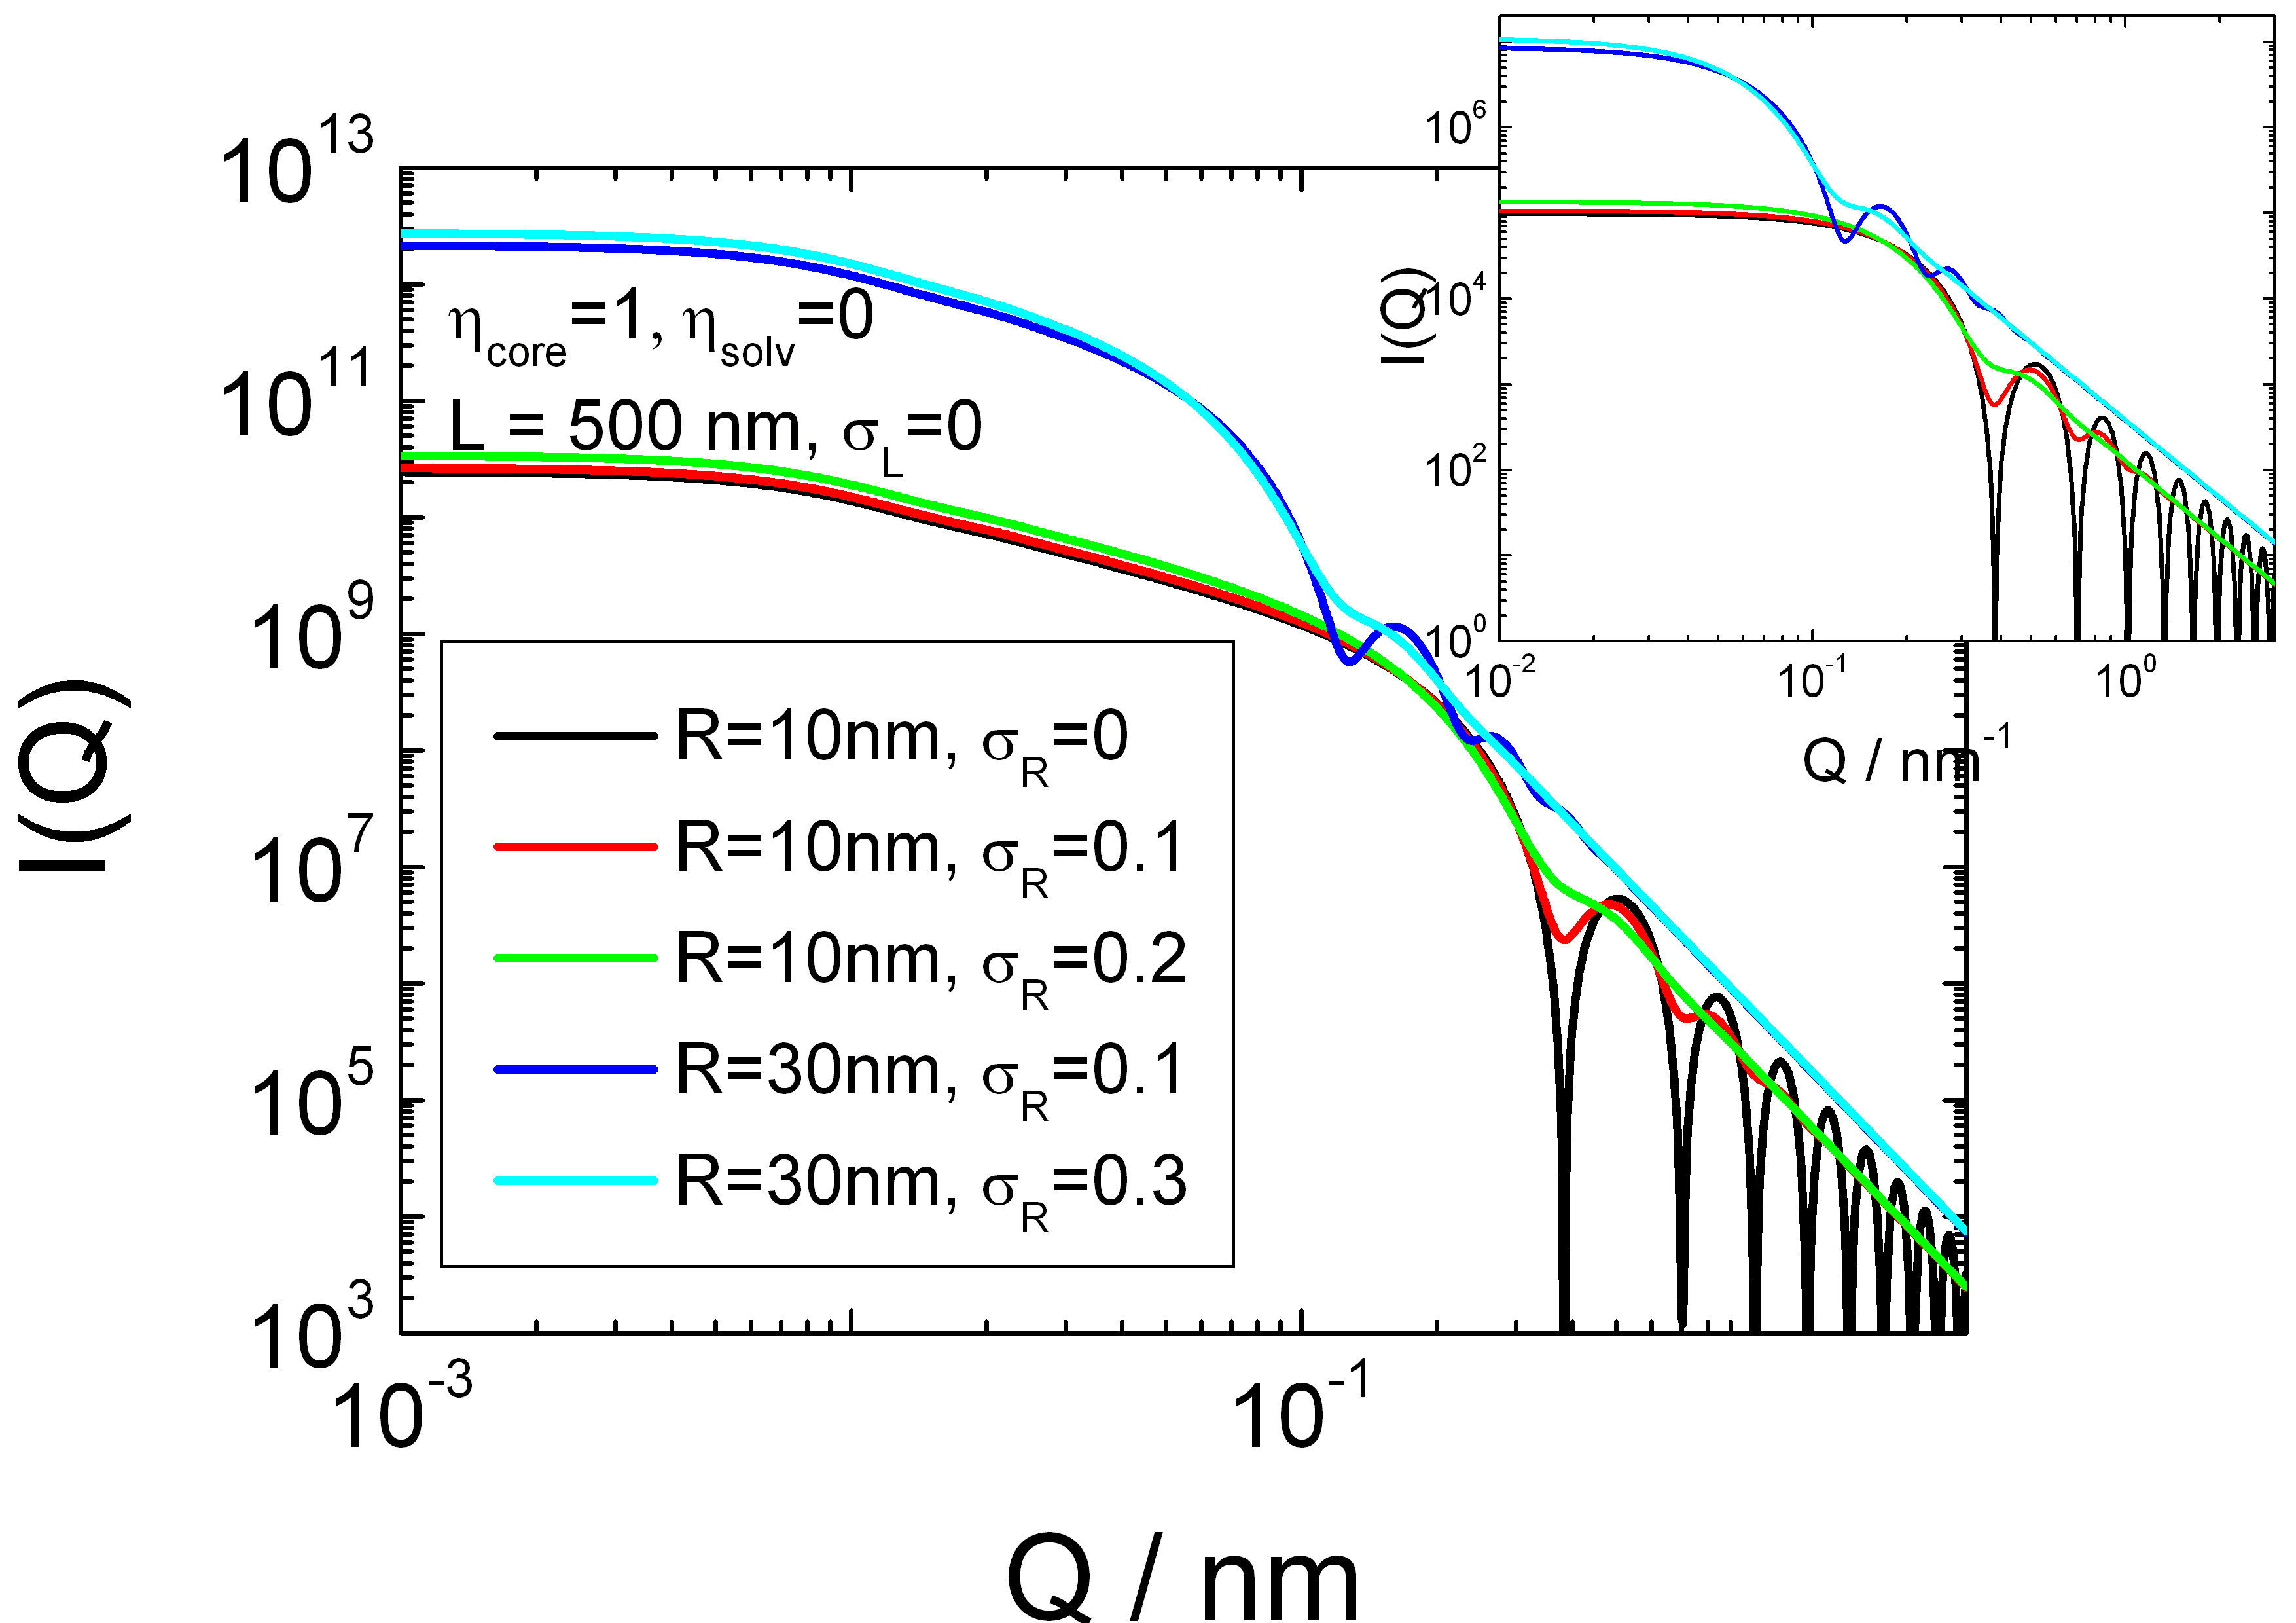
\includegraphics[width=0.8\textwidth,height=0.55\textwidth]{../images/form_factor/anisotropic/CylindricalHomogeneousXSIQ.png}
\end{center}
\caption{Scattering curve for the form factor "\texttt{Pcs:homogeneousCyl}" only (insert) and
in combination with a structure factor "\texttt{P'(Q): Thin Rod}".}
\label{fig_IQ:Pcs:CylindricalHomogeneousXSIQ}
\end{figure}

\clearpage
\subsubsection{Pcs(Q) for cross-section of a cylindrical shell with elliptical cross section} ~\\
\label{plugin:Pcs:CylEllSh}

\noindent
This cross-section form factor describes the scattering of an elliptical core-shell cross-section.
The cross-section radius $R$ can have a distribution with a width of $sigma$ as
described by a log-normal distribution according to eq.\ \ref{eq:LogNormal}.

\begin{equation}
\begin{split}
    P_\textrm{cs}(Q) = & \int_0^\infty \textrm{LogNorm}(x,1,\sigma_{R},1,R)  \quad \times\\
        & \int_0^{\pi/2}
\Big[\left( \eta_\textrm{shell}-\eta_\textrm{solv}\right)F_\textrm{cs,ell}(Q,R+t,\epsilon,\phi) \\
& \quad + \left(\eta_\textrm{core}-\eta_\textrm{shell}\right)F_\textrm{cs,ell}(Q,R,\epsilon,\phi)
\Big]^2 \, \mathrm{d}\phi
\end{split}
\end{equation}
with
\begin{subeqnarray}
F_\textrm{cs,ell}\left(Q,R,\epsilon,\Delta\eta\phi\right) &=&  \frac{2 \mathrm{J}_1(Qr(R,\epsilon,\phi))}{Qr(R,\epsilon,\phi)}   \\
r(R,\epsilon,\phi) &=& R\sqrt{\sin^2\phi+\epsilon^2\cos^2\phi}
\end{subeqnarray}



\noindent
\textbf{Input parameters for \texttt{Pcs:homogeneousCyl}:}
\begin{description}
    \item[\texttt{R}] most probable radius $R$
    \item[\texttt{sigm\_R}] width $\sigma_R$ of radius distribution (LogNorm)
    \item[\texttt{epsilon}] eccentricity $\epsilon$ of ellipyical cross-section
    \item[\texttt{t}] shell thickness $t$
    \item[\texttt{dummy}] not used
    \item[\texttt{dummy}] not used
    \item[\texttt{dummy}] not used
    \item[\texttt{eta\_core}] scattering length density of the core $\eta_\textrm{core}$
    \item[\texttt{eta\_shell}] scattering length density of the shell $\eta_\textrm{shell}$
    \item[\texttt{eta\_solv}] scattering length density of the solvent $\eta_\textrm{solv}$
\end{description}

\noindent
\textbf{Note}
\begin{itemize}
  \item This form factor is supposed to be combined with a shape factor for
local cylindrical objects which are implemented as structure  plugins
under "\texttt{[by plugin|anisotropic obj.|P'(Q): local cylindrical obj.]}".
\item As the form factor already has the width distribution included one normally uses in \SASfit as a size distribution
the \texttt{Delta}-distribution.
\end{itemize}

\clearpage
\subsection{P'(Q) for local planar obj.} ~\\
\label{plugin:Pprime4planar}



\clearpage
\subsubsection{P'(Q): thin discs} ~\\
\label{plugin:Pprime4Discs}

\begin{figure}[htb]
\begin{center}
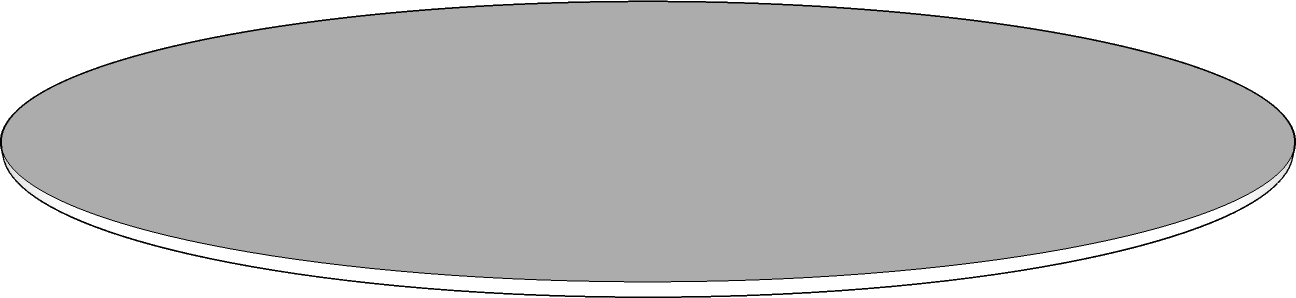
\includegraphics[width=0.686\textwidth,height=0.27\textwidth]{../images/form_factor/anisotropic/ThinDisc.png}
\end{center}
\caption{Sketch of a thin disc with a radius $R$. The thickness of the disc is assumed to be much smaller than its radius.}
\label{fig:ThinDisc}
\end{figure}

\noindent
\textbf{Input parameters for \texttt{P'(Q): Thin Disc}:}
\begin{description}
    \item[\texttt{R}] most probable radius $R$
    \item[\texttt{dummy}] not used
    \item[\texttt{sima}] width $\sigma$ of radius distribution (LogNorm)
\end{description}

\noindent
\textbf{Note}
\begin{itemize}
  \item This structure factor is supposed to be combined with a form factor of local planar objects which are implemented as form factor plugins
under "\texttt{[by plugin|anisotropic obj.|Pcs(Q): local planar obj.]}".
\item The structure factor already has a log-normal width distribution for one parameter included.
\end{itemize}

\begin{figure}[htb]
\begin{center}
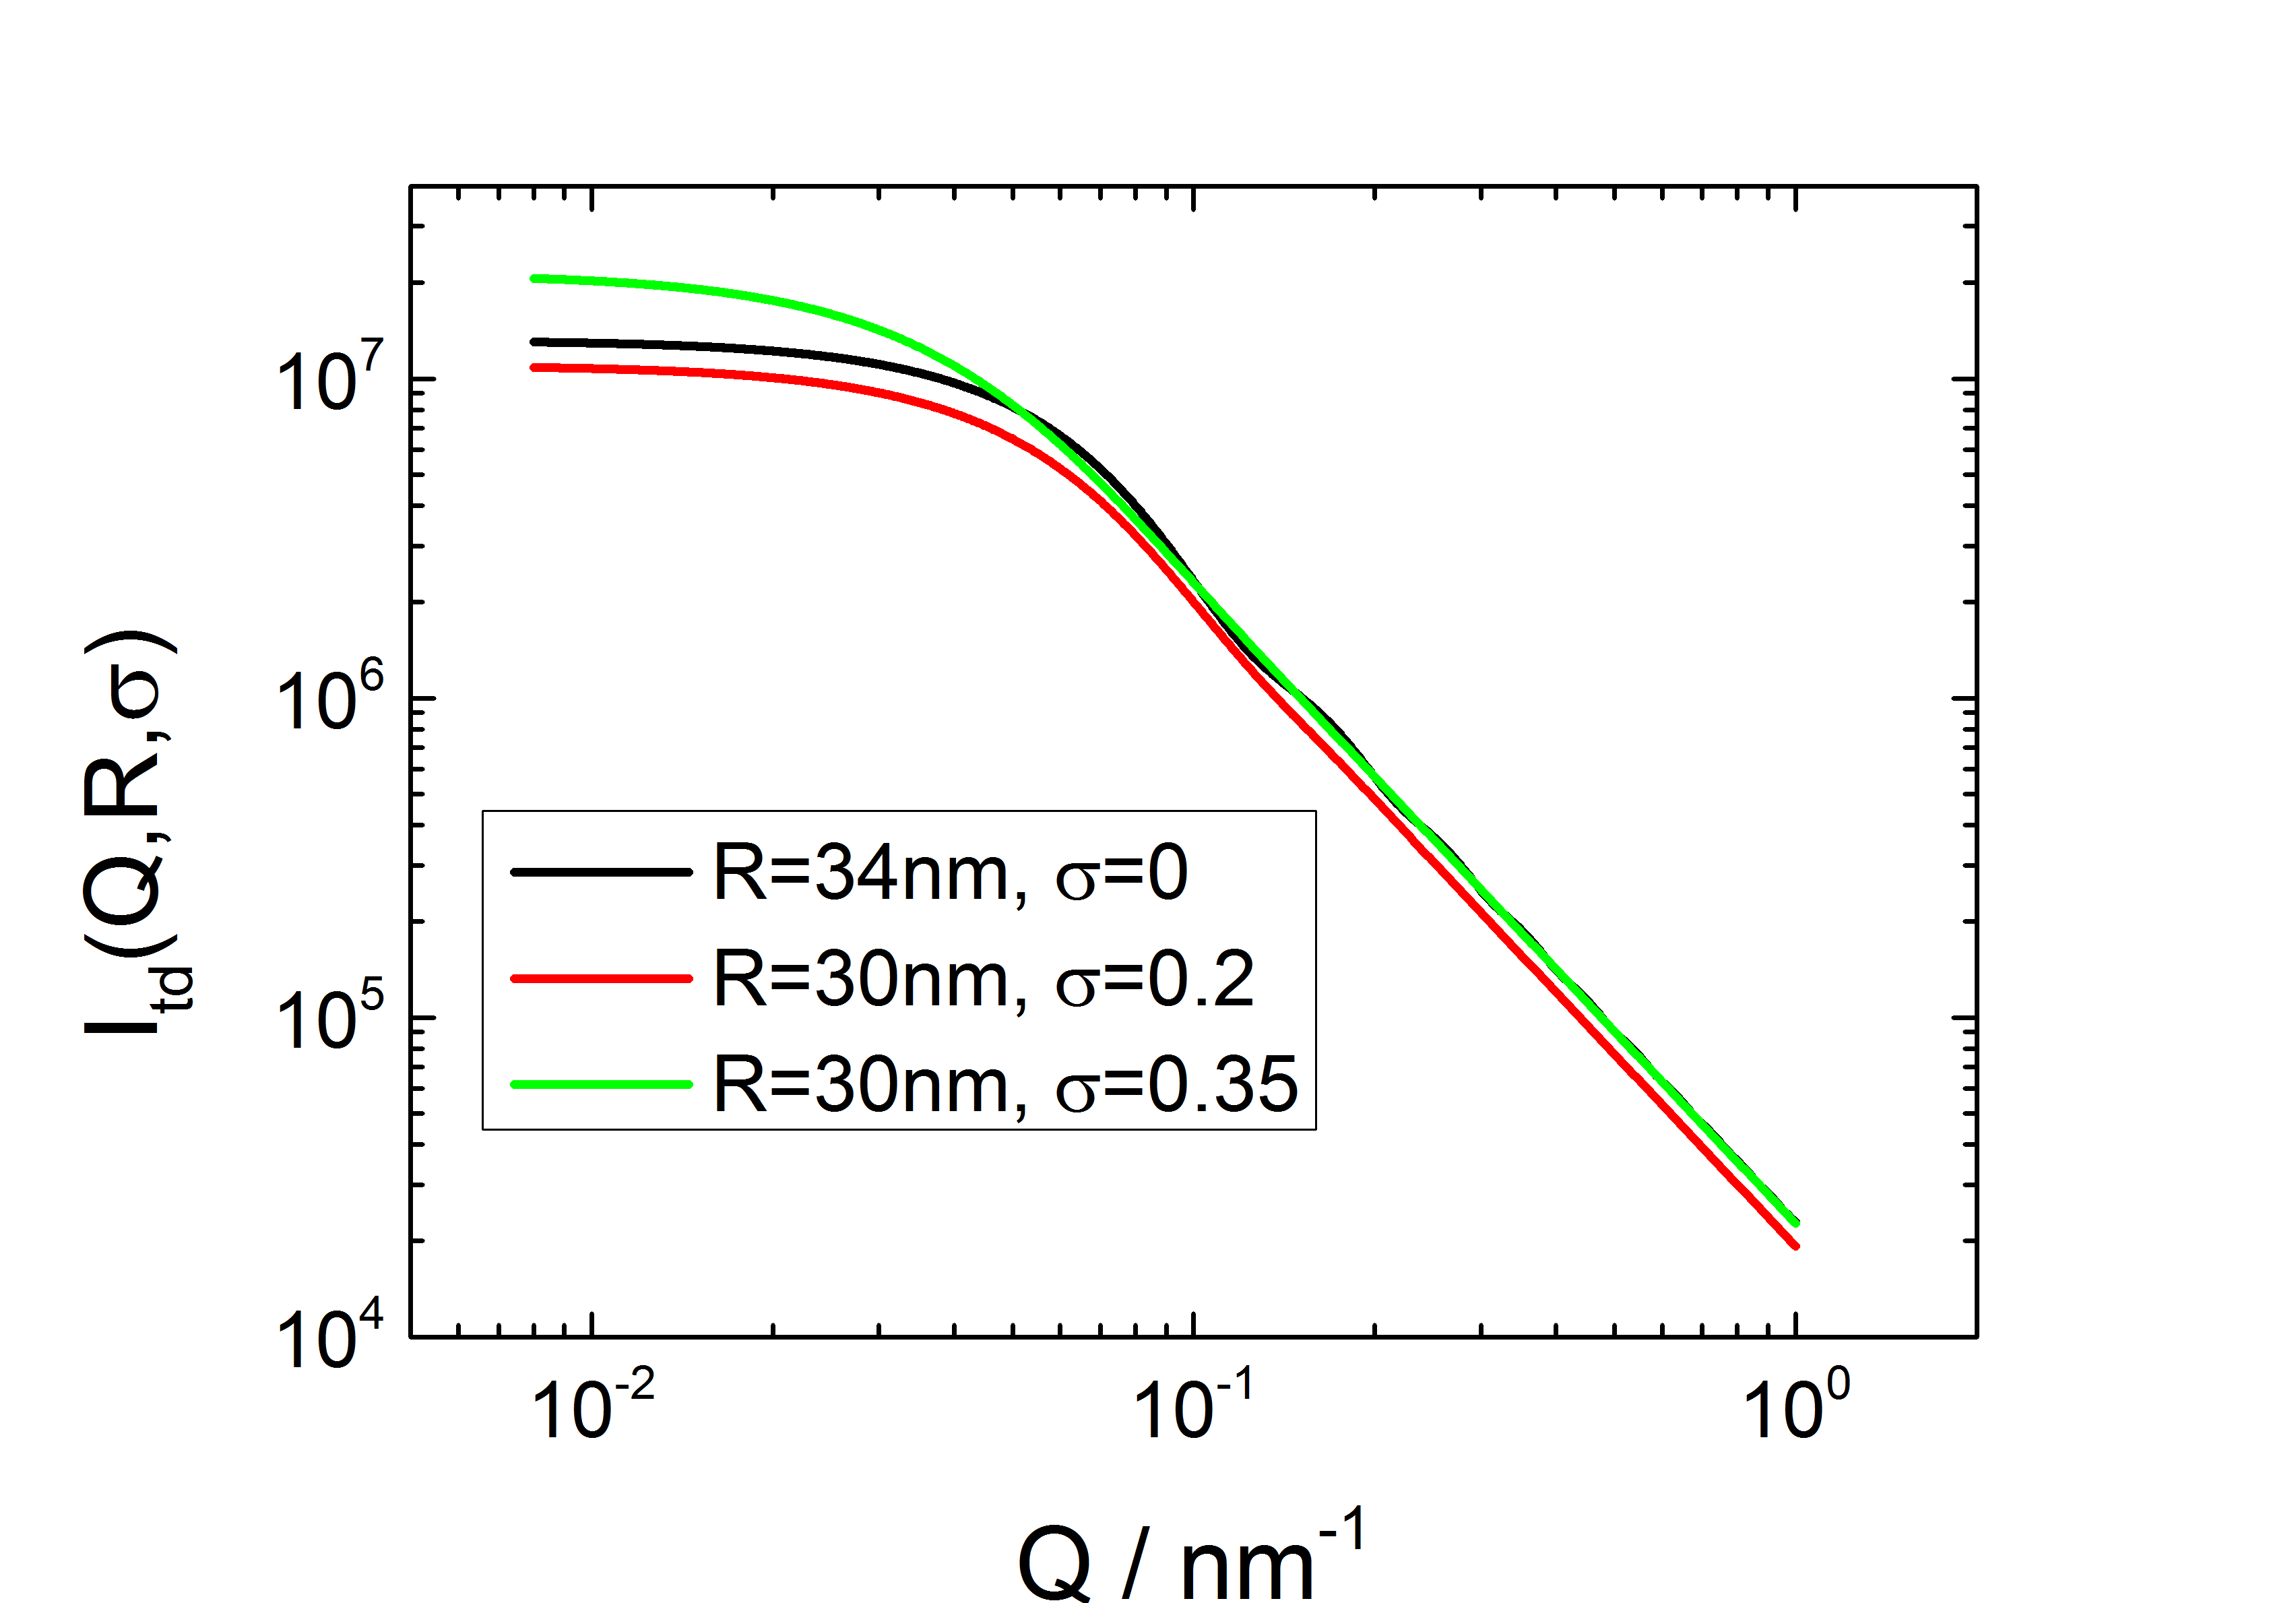
\includegraphics[width=0.8\textwidth,height=0.55\textwidth]{../images/form_factor/anisotropic/PprimeThinDisc.png}
\end{center}
\caption{Scattering curve for the structure factor "\texttt{P'(Q): Thin Disc}" in combination with a constant background of 1".}
\label{fig_IQ:PprimeThinDisc}
\end{figure}

\clearpage
\subsubsection{P'(Q): thin spherical shell} ~\\
\label{plugin:Pprime4spShell}

\begin{figure}[htb]
\begin{center}
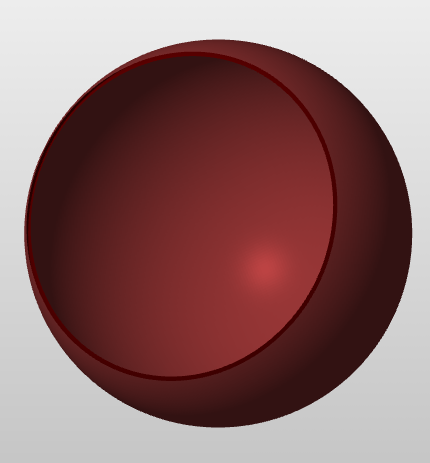
\includegraphics[width=0.43\textwidth,height=0.463\textwidth]{../images/form_factor/anisotropic/Sphere_thin.png}
\end{center}
\caption{Sketch of a thin spherical shell with a radius $R$. The thickness of the shell is assumed to be much smaller than the radius of the sphere.}
\label{fig:ThinSphericalShell}
\end{figure}

\noindent
\textbf{Input parameters for \texttt{P'(Q): Thin Spherical Shell}:}
\begin{description}
    \item[\texttt{R}] most probable radius $R$
    \item[\texttt{dummy}] not used
    \item[\texttt{sima}] width $\sigma$ of radius distribution (LogNorm)
\end{description}

\noindent
\textbf{Note}
\begin{itemize}
  \item This structure factor is supposed to be combined with a form factor of local planar objects which are implemented as form factor plugins
under "\texttt{[by plugin|anisotropic obj.|Pcs(Q): local planar obj.]}".
\item The structure factor already has a log-normal width distribution for one parameter included.
\end{itemize}

\begin{figure}[htb]
\begin{center}
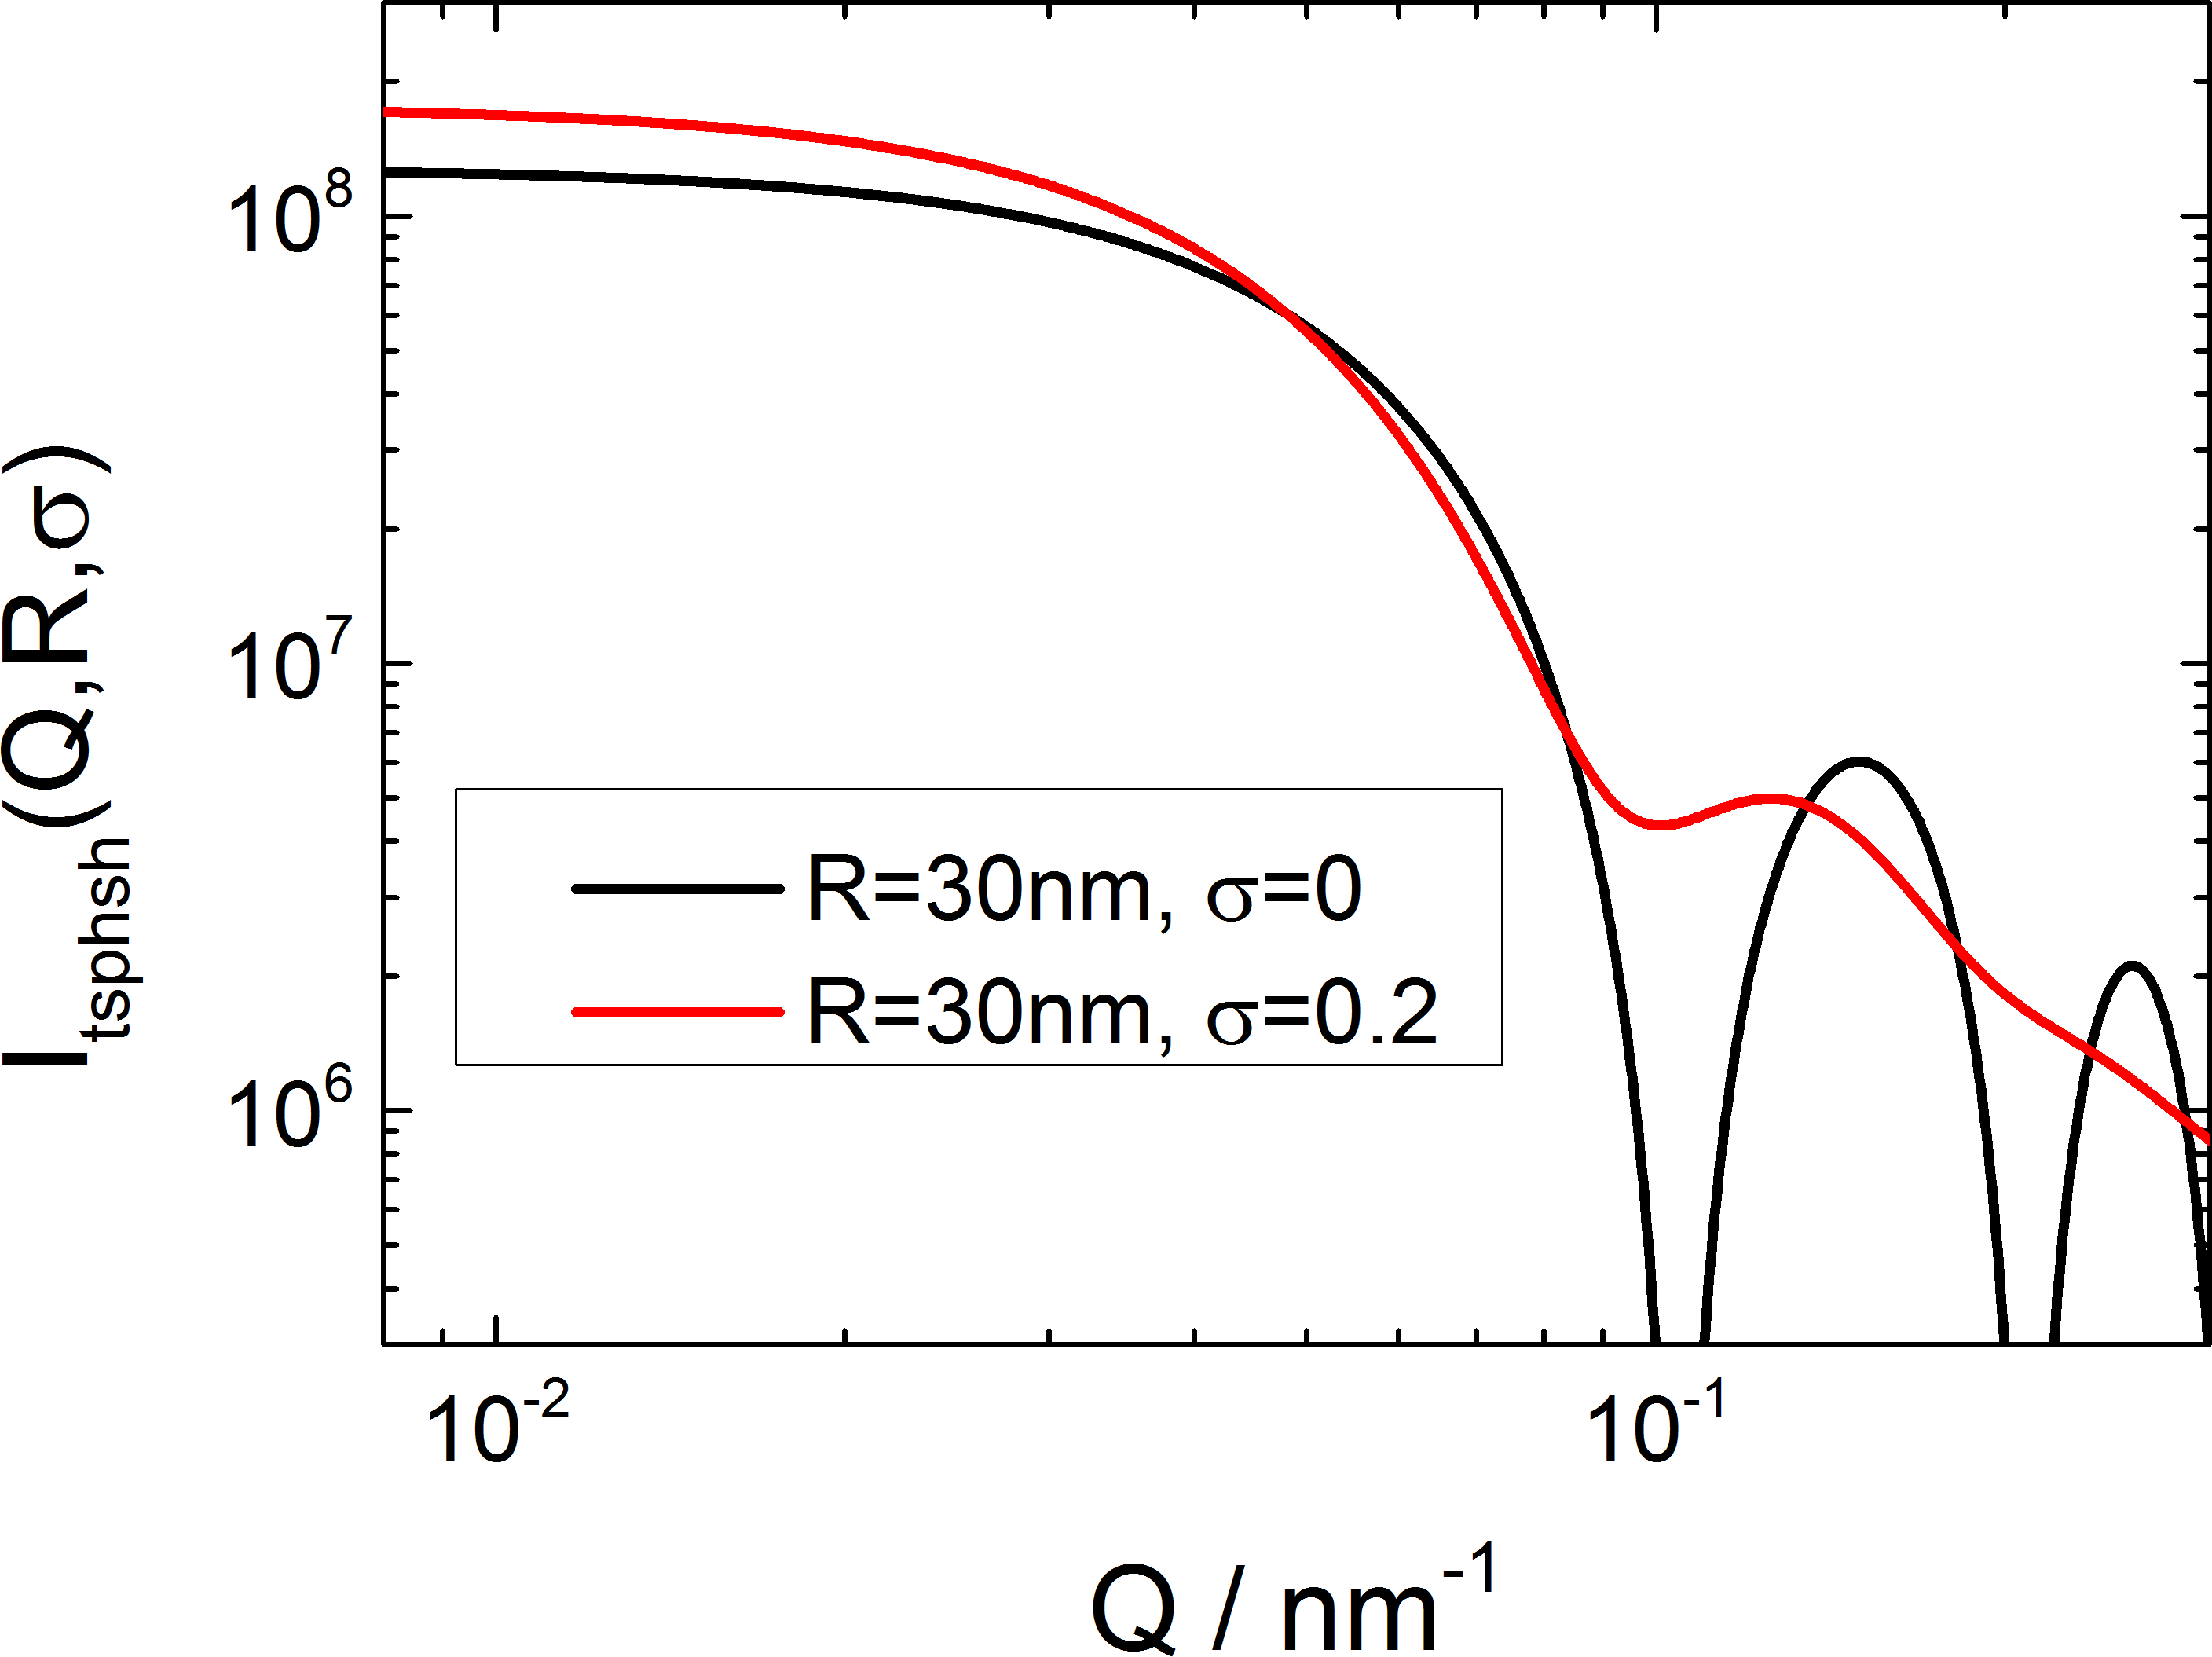
\includegraphics[width=0.8\textwidth,height=0.55\textwidth]{../images/form_factor/anisotropic/PprimeThinSphShell.png}
\end{center}
\caption{Scattering curve for the structure factor "\texttt{P'(Q): Thin Spherical Shell}" in combination with a constant background of 1".}
\label{fig_IQ:PprimeThinSphShell}
\end{figure}


\clearpage
\subsubsection{P'(Q): thin ellipsoidal shell} ~\\
\label{plugin:Pprime4ellShell}

\begin{figure}[htb]
\begin{center}
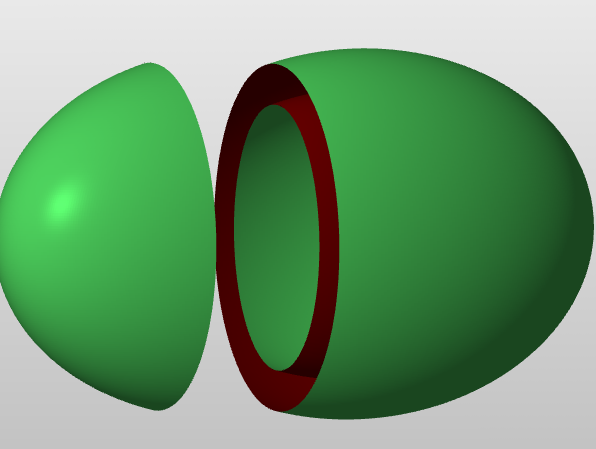
\includegraphics[width=0.596\textwidth,height=0.449\textwidth]{../images/form_factor/anisotropic/Ellipsoid_hollow.png}
\end{center}
\caption{Sketch of a thin ellipsoidal shell with a radius $R$ and eccentricity $\epsilon$. The thickness of the shell is assumed to be much smaller than the two radii of the elliptical shell.}
\label{fig:ThinEllipsoidalShell}
\end{figure}

\noindent
\textbf{Input parameters for \texttt{P'(Q): Thin Ellipsoidal Shell}:}
\begin{description}
    \item[\texttt{R}] most probable radius $R$
    \item[\texttt{epsilon}] eccentricity $\epsilon$
    \item[\texttt{sima\_R}] width $\sigma_R$ of radius distribution (LogNorm)
\end{description}

\noindent
\textbf{Note}
\begin{itemize}
  \item This structure factor is supposed to be combined with a form factor of local planar objects which are implemented as form factor plugins
under "\texttt{[by plugin|anisotropic obj.|Pcs(Q): local planar obj.]}".
\item The structure factor already has a log-normal width distribution for one parameter included.
\end{itemize}

\begin{figure}[htb]
\begin{center}
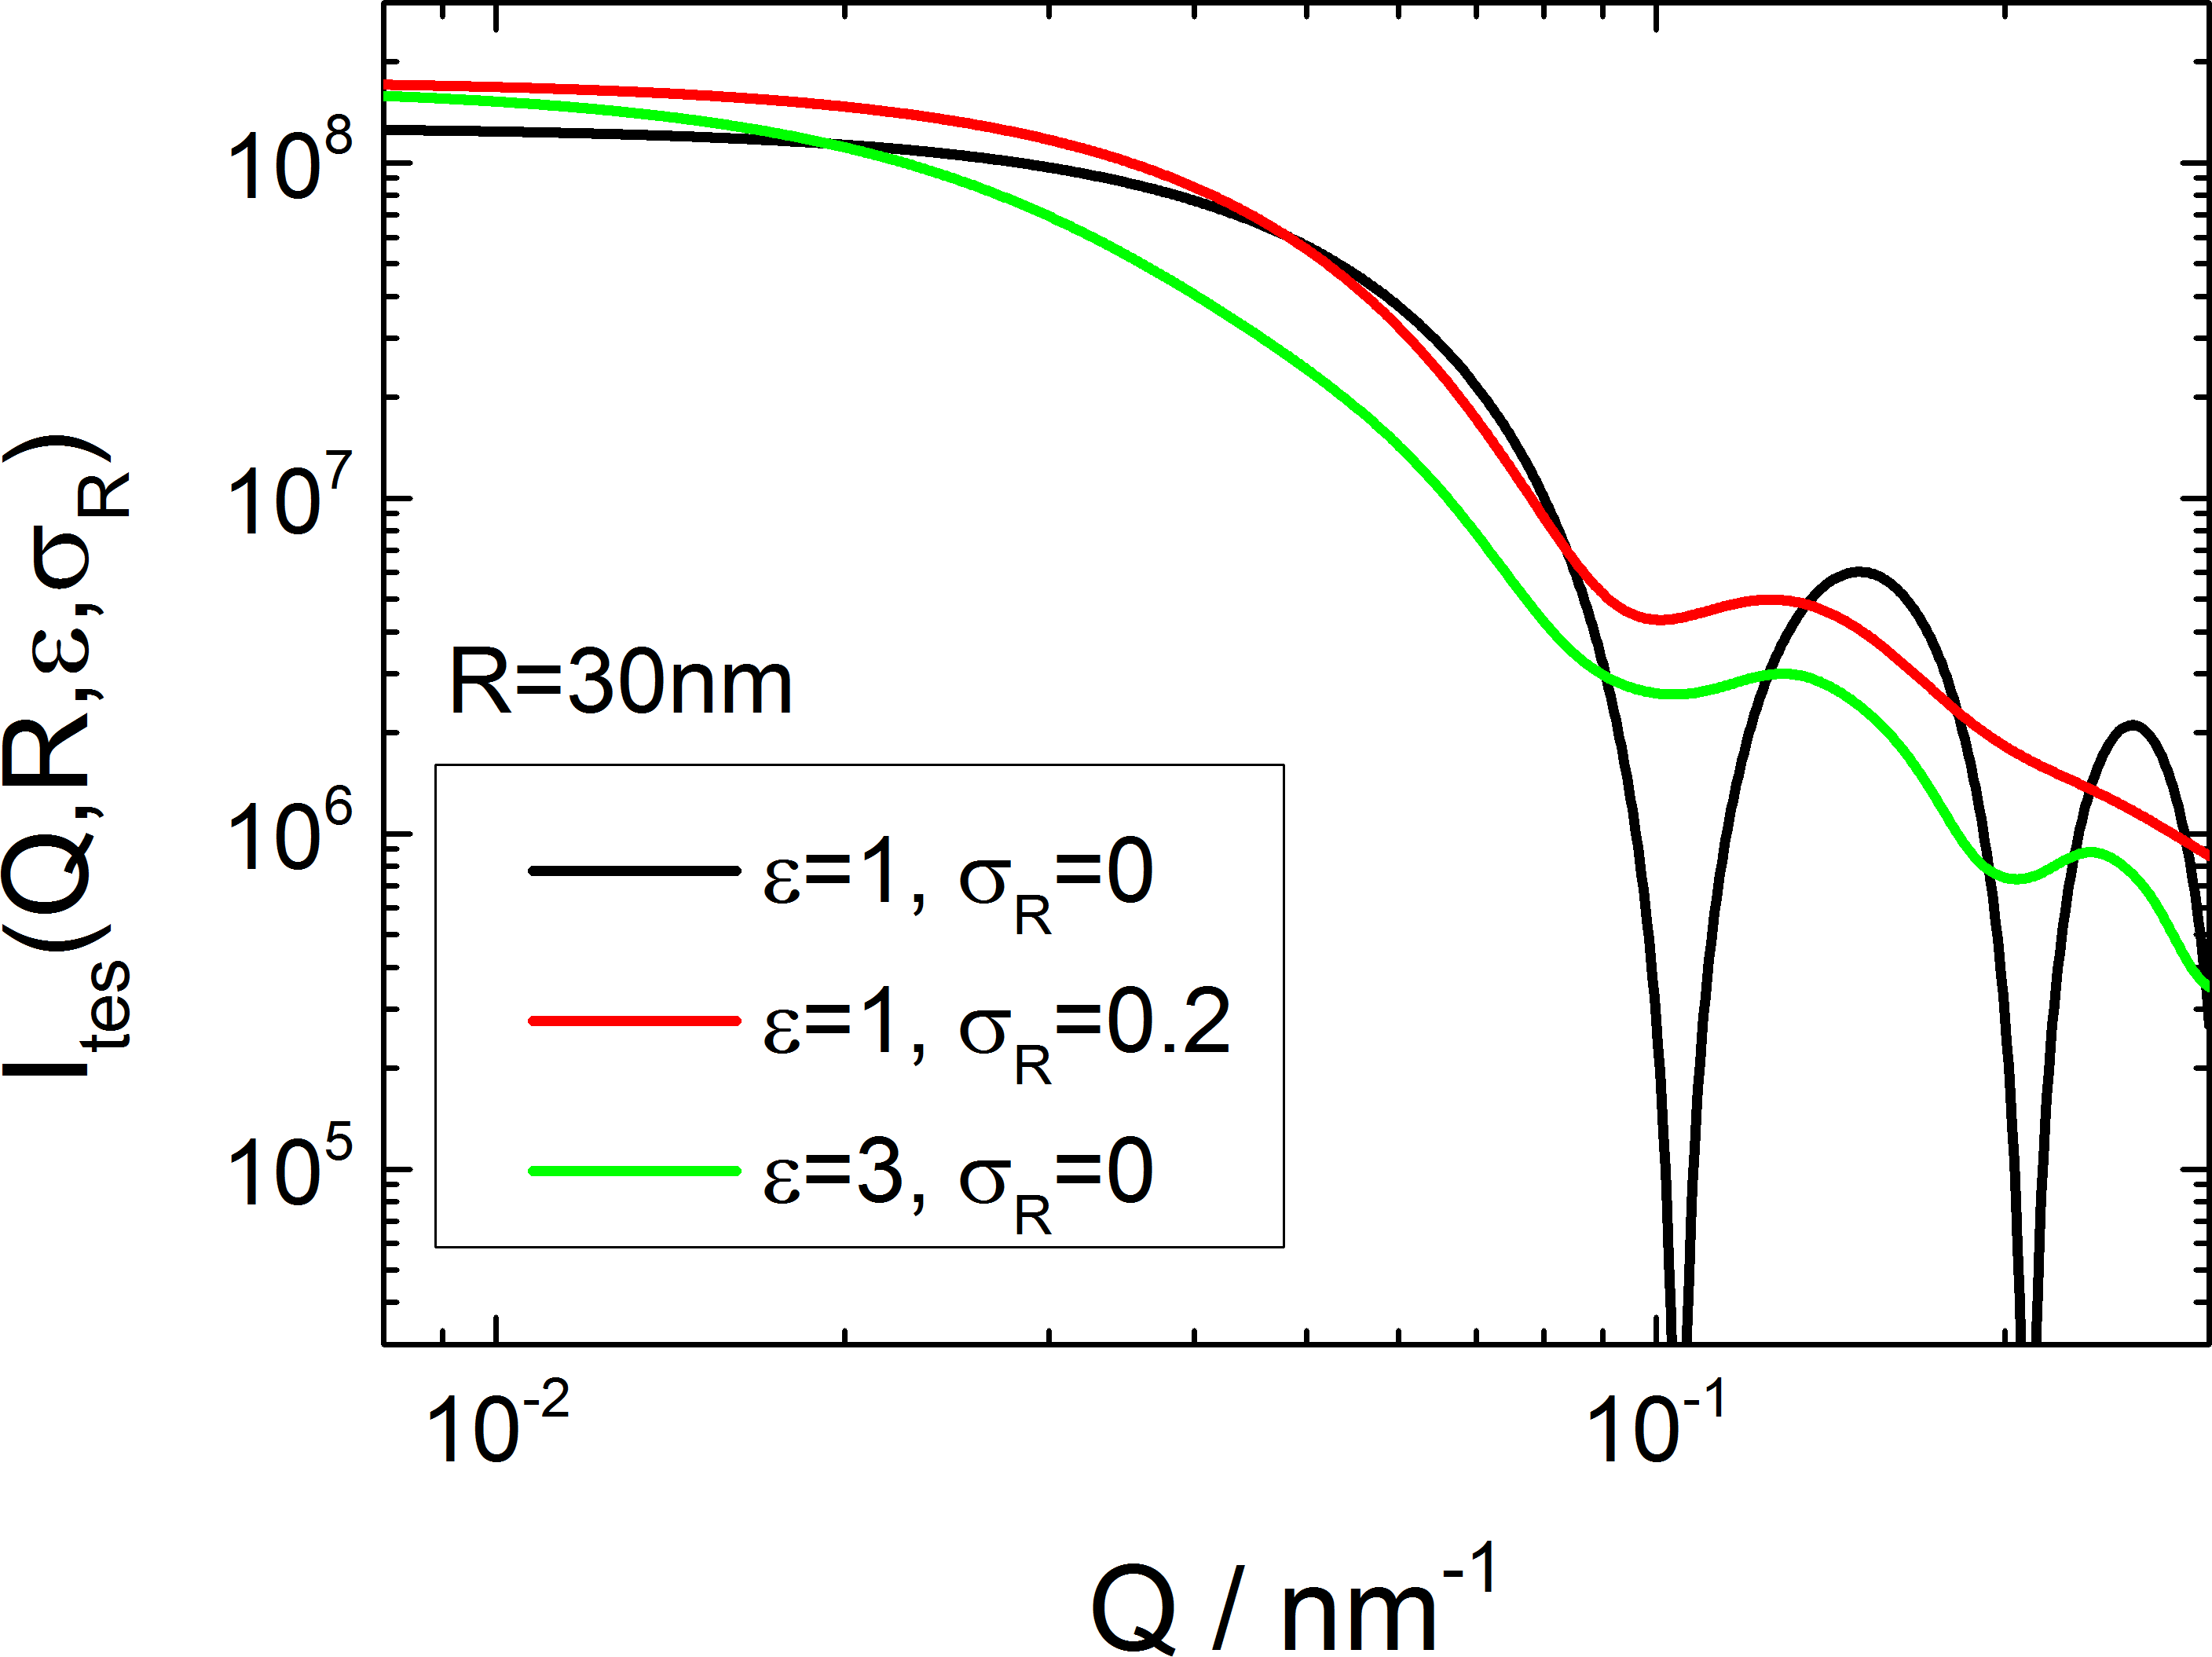
\includegraphics[width=0.8\textwidth,height=0.55\textwidth]{../images/form_factor/anisotropic/PprimeThinEllShell.png}
\end{center}
\caption{Scattering curve for the structure factor "\texttt{P'(Q): Thin Ellipsoidal Shell}" in combination with a constant background of 1".}
\label{fig_IQ:PprimeThinEllShell}
\end{figure}

\clearpage
\subsubsection{P'(Q): thin hollow cylinder} ~\\
\label{plugin:Pprime4hollowcylinder}

\begin{figure}[htb]
\begin{center}
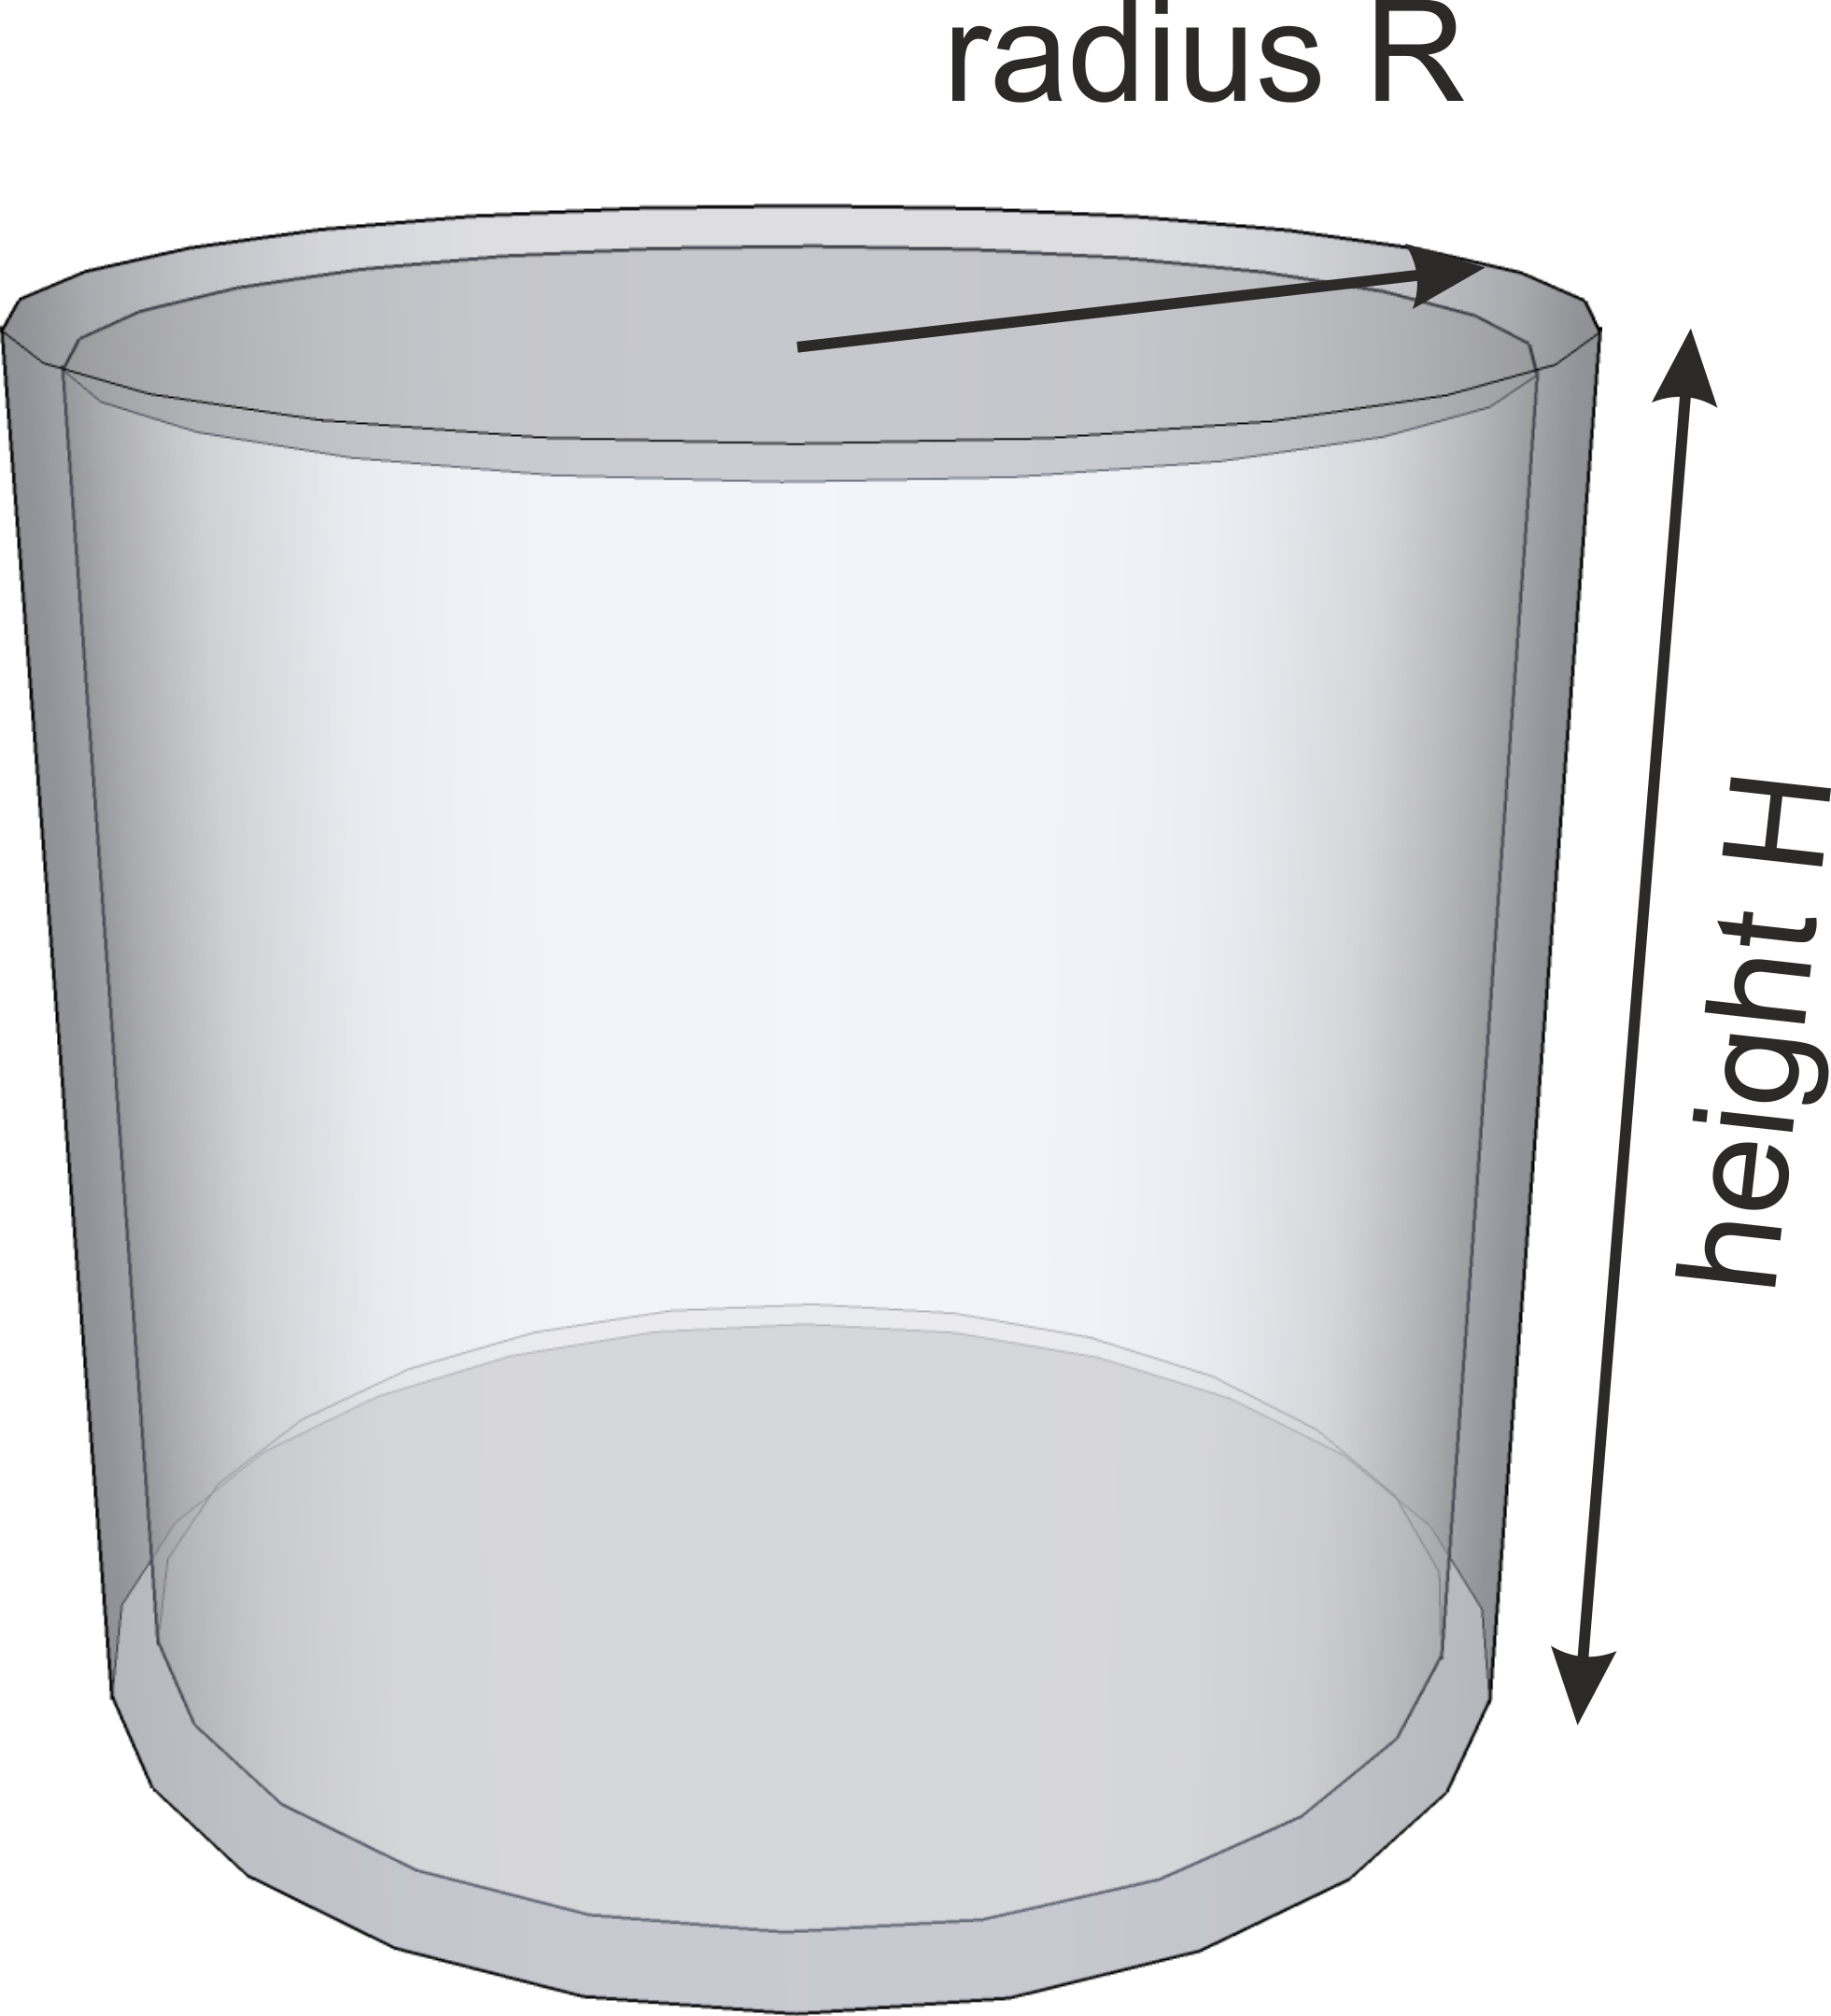
\includegraphics[width=0.3922\textwidth,height=0.4318\textwidth]{../images/form_factor/anisotropic/ThinHollowCylinder.png}
\end{center}
\caption{Sketch of a thin hollow cylinder of height $H$ and radius $R$. The thickness of the wall is assumed to be much smaller than the outer dimensions of the cylinder.}
\label{fig:ThinHollowCylinder}
\end{figure}

\begin{align}
\begin{split}
\Xi(Q,R,H,\alpha) & = 2\pi R
\left[ R \frac{J_1\left(Q R \sin\alpha\right)}{Q R \sin\alpha} \right. \\
& \left. \quad \quad + H J_0\left( \frac{QH}{2} \cos\alpha\right)\frac{\sin\left(\frac{QH}{2} \cos\alpha\right)}{\frac{QH}{2} \cos\alpha} \right]
\end{split} \\
P_\text{thc}(Q,R,H) &= \int_0^{\pi/2} \Xi^2(Q,R,H,\alpha) \sin\alpha \mathrm{d}\alpha \\
\begin{split}
I_{thc}(Q,R,H) &= \int_0^\infty \int_0^\infty
\mathrm{LogNorm}(r,1,\sigma_R,1,R,1) \\
& \qquad \qquad  \mathrm{LogNorm}(h,1,\sigma_H,1,H,1) P_\text{thc}(Q,r,h)
\, \mathrm{d}h \, \mathrm{d}r
\end{split}
\end{align}

\noindent
\textbf{Input parameters for \texttt{P'(Q): Thin Hollow Cylinder}:}
\begin{description}
    \item[\texttt{R}] most probable cylinder radius $R$
    \item[\texttt{H}] most probable cylinder height $H$
    \item[\texttt{sima\_R}] width $\sigma_R$ of radius distribution (LogNorm)
    \item[\texttt{sima\_H}] width $\sigma_H$ of height distribution (LogNorm)
\end{description}

\noindent
\textbf{Note}
\begin{itemize}
  \item This structure factor is supposed to be combined with a form factor of local planar objects which are implemented as form factor plugins
under "\texttt{[by plugin|anisotropic obj.|Pcs(Q): local planar obj.]}".
\item The structure factor already has a log-normal width distribution for one parameter included.
\end{itemize}

\begin{figure}[htb]
\begin{center}
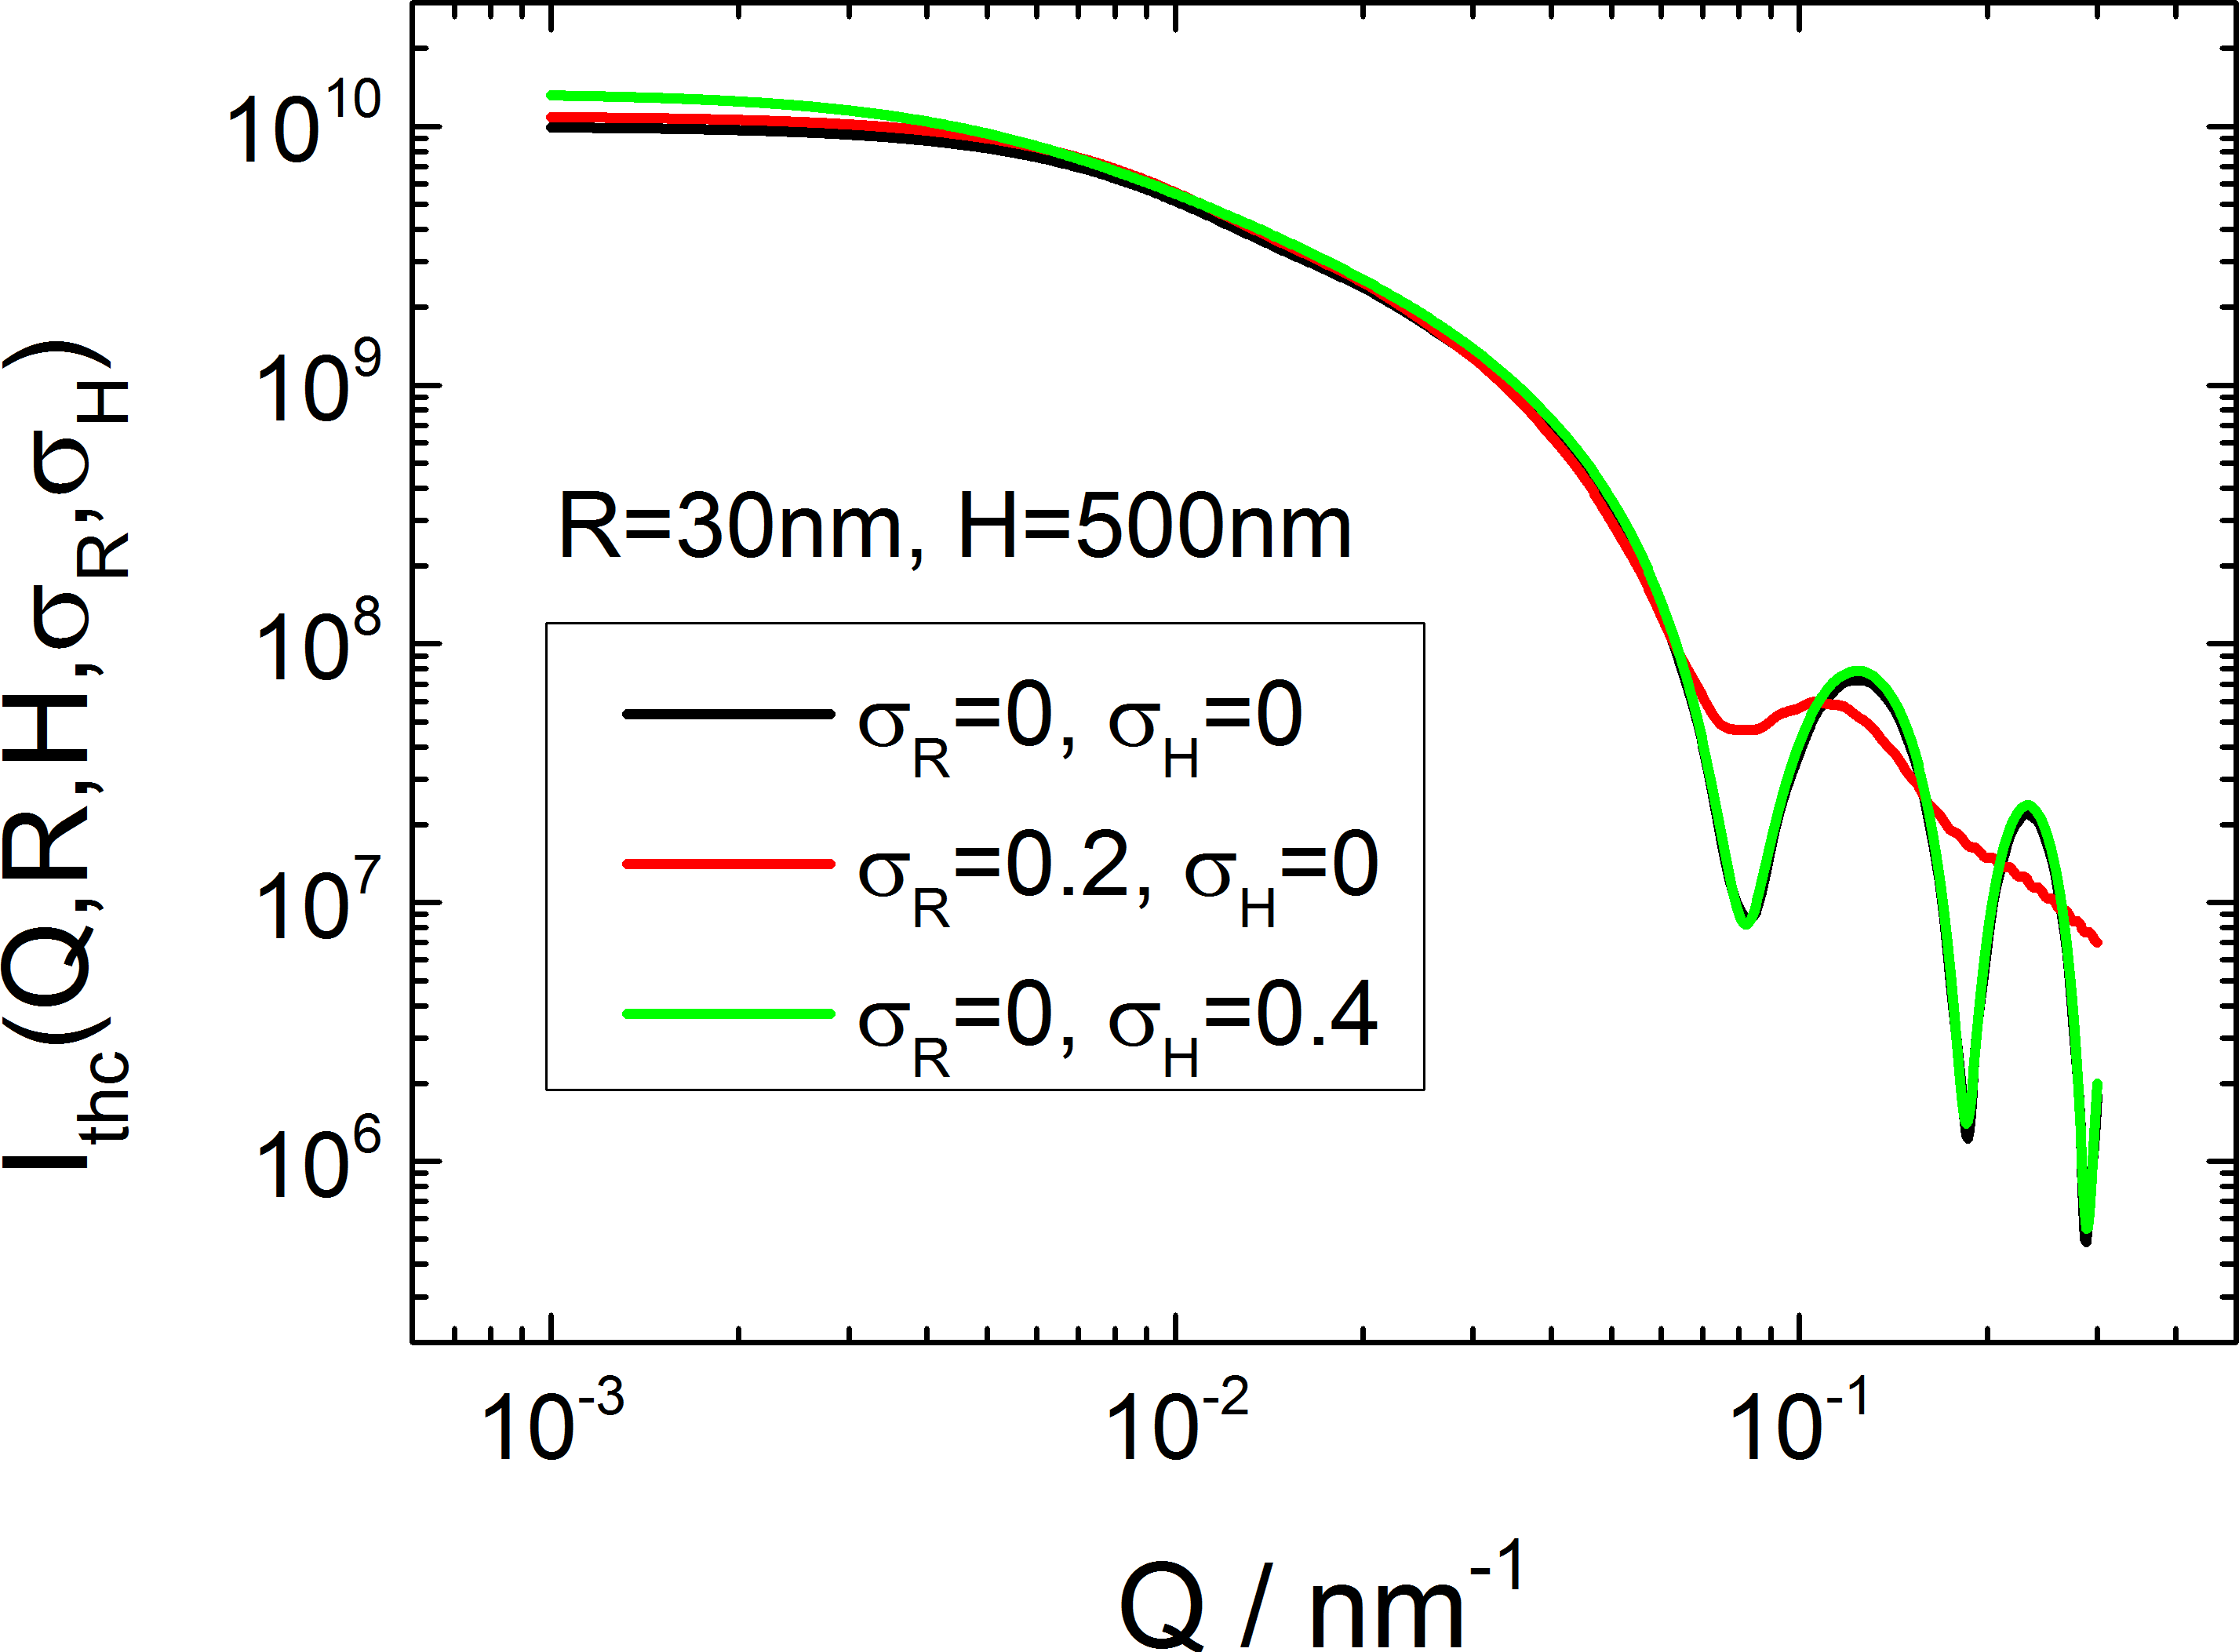
\includegraphics[width=0.8\textwidth,height=0.55\textwidth]{../images/form_factor/anisotropic/PprimeThinHollowCylinder.png}
\end{center}
\caption{Scattering curve for the structure factor "\texttt{P'(Q): Thin Hollow Cylinder}" in combination with a constant background of 1".}
\label{fig_IQ:PprimeThinHollowCylinder}
\end{figure}


\clearpage
\subsection{P'(Q) for local cylindrical obj.} ~\\
\label{plugin:Pprime4cylindrical}


\clearpage
\subsubsection{P'(Q): rods} ~\\
\label{plugin:Pprime4rods}

\begin{figure}[htb]
\begin{center}
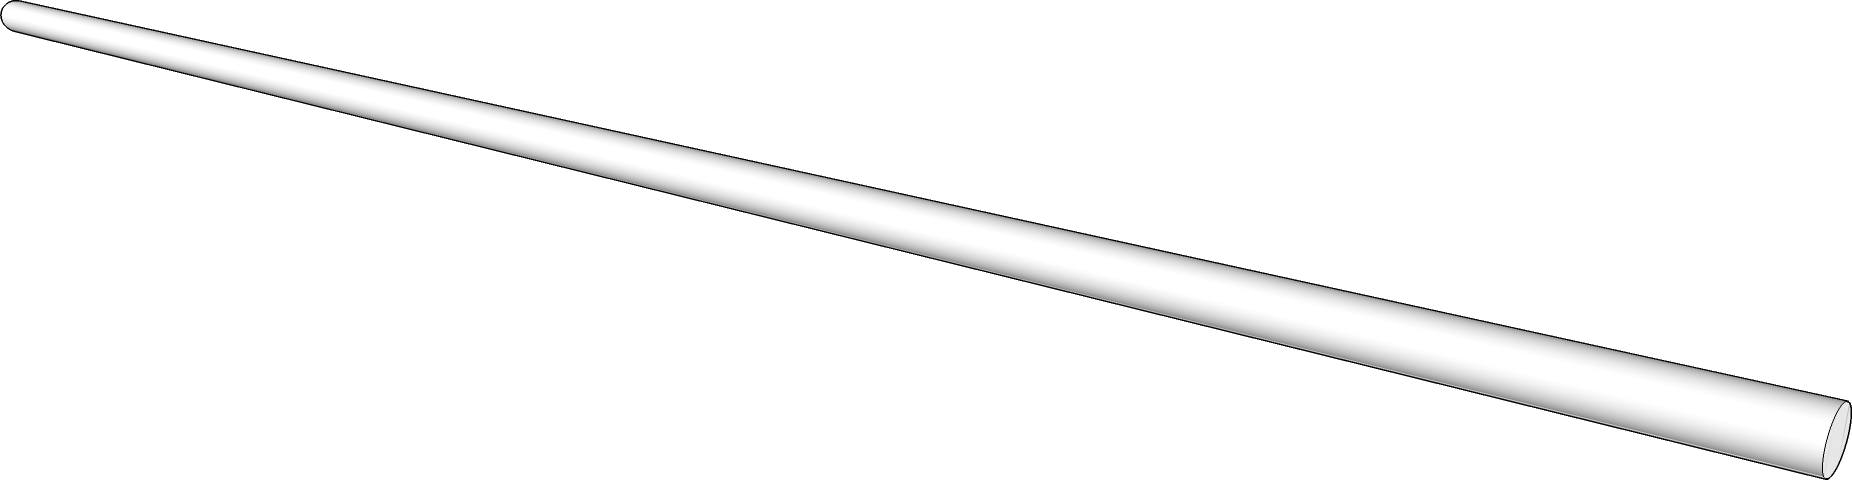
\includegraphics[width=0.926\textwidth,height=0.24\textwidth]{../images/form_factor/anisotropic/ThinRod.png}
\end{center}
\caption{Sketch of a thin Rod of Length $L$. The diameter of the rod is assumed to be much smaller than its length.}
\label{fig:ThinRod}
\end{figure}

\noindent
\textbf{Note}
\begin{itemize}
  \item This structure factor is supposed to be combined with a form factor with local cylindrical geometry which are implemented as form factor plugins
under "\texttt{[by plugin|anisotropic obj.|Pcs(Q): local cylindrical obj.]}".
\item The structure factor already has a log-normal width distribution for one parameter included.
\end{itemize}

\clearpage
\subsubsection{P'(Q): Kholodenko's worm} ~\\
\label{plugin:Pprime4kohlodenko}

\begin{figure}[htb]
\begin{center}
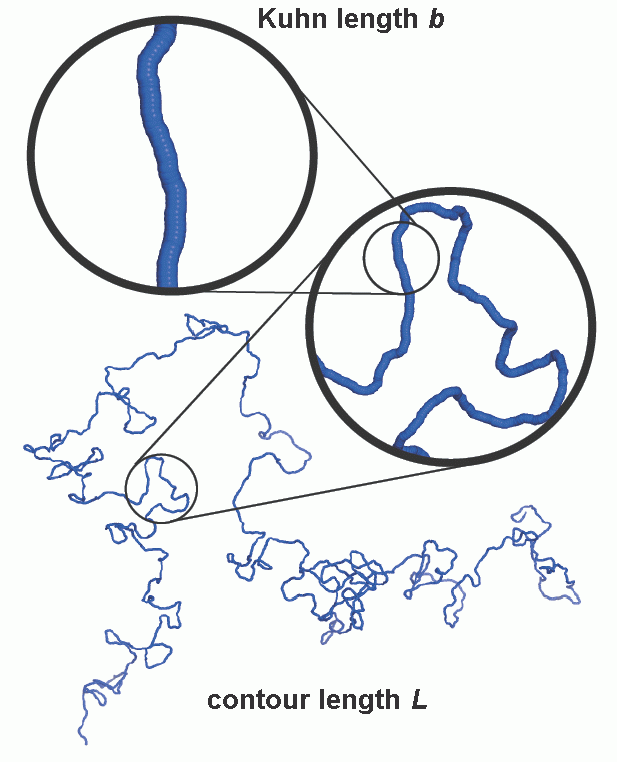
\includegraphics[width=0.617\textwidth,height=0.762\textwidth]{SemiflexiblePolymerTxt.png}
\end{center}
\caption{}
\label{fig:KholodenkoWorm}
\end{figure}

By using the analogy between Dirac�s fermions
and semi-flexible polymers
Kholodenko \cite{kholodenko93} could give a simple expression for the
scattering behaviour of wormlike structures. The form factor $P_0(Q)$ resulting
from Kholodenko�s approach is designed to reproduce
correctly the rigid-rod limit and the random-coil limit.
Defining $x = 3L/l_b$ ($L$: contour length, $l_b$: Kuhn length), it is given by
\begin{align}
P_0(Q,L,l) &= \frac{2}{x} \left[I_{(1)} -\frac{1}{x}I_{(2)}\right]
\label{eq:KholodenkoPprime}
\end{align}
where
\begin{align}
I_{(n)}(x) &= \int_0^x  f(z) \, z^{n-1} \, dz
\end{align}
together with
\begin{align}
f(z)) &=
\begin{cases} \displaystyle
\frac{1}{E}\frac{\sinh(Ez)}{\sinh(z)} & \text{for} \quad \displaystyle Q \leq \frac{3}{l}\\ \\
\displaystyle
\frac{1}{F}\frac{\sin(Fz)}{\sinh(z)} & \text{for} \quad \displaystyle Q > \frac{3}{l}
\end{cases}
\end{align}
and
\begin{align}
E = \sqrt{1-\left(\frac{lQ}{3}\right)^2} \quad \text{and} \quad F = \sqrt{\left(\frac{lQ}{3}\right)^2-1}
\end{align}

\begin{align}
P(Q,L,l_b,R) = P_0(Q,L,l_b)\, P_{cs}(Q,R)
\end{align}

\vspace{5mm}

\hspace{1pt}\\
\underline{Input Parameters for model \texttt{P'(Q) Kholodenko Worm}:}\\
\begin{description}
\item[\texttt{lb}] Kuhn length\footnote{The Kuhn length $l_b$ is related to the length $a$ of
    locally stiff segment simply via $l_b=2a$} $l$ of semi-flexible worm-like structure
\item[\texttt{L}] contour length $L$ of semi-flexible worm-like structure
\end{description}

\noindent
\textbf{Note}
\begin{itemize}
  \item This structure factor is supposed to be combined with a form factor with local cylindrical geometry which are implemented as form factor plugins
under "\texttt{[by plugin|anisotropic obj.|Pcs(Q): local cylindrical obj.]}".
\item The structure factor already has a log-normal width distribution for one parameter included.
\item The equivalent solution of J.S. Pedersen \cite{Pedersen96Macrom} would be the expressions of wormlike structures without excluded volume effects.
\end{itemize}

\clearpage
\subsubsection{P'(Q): wormlike PS1} ~\\
\label{plugin:Pprime4wormPS1}

For worm-like micelles J.S. Pedersen \cite{Pedersen96Macrom} has developed three models
for worm-like micelles, from which one is basing on a method developed by Yoshizaki et al.\ \cite{Yoshizaki1980}.

\paragraph*{\textbf{Without Excluded Volume Effects.}}
This first of the three solutions given by J.S. Pedersen \cite{Pedersen96Macrom} for
worm-like micelles starts from the expression for the scattering function as follows:
\begin{align}
\label{eq:SWC}
\begin{split}
S_\text{WC}(Q,L,l_B) &= L^2 \left[  \left(1-\chi(Q,L,l_B)\right)
            S_\text{chain}(Q,L,l_B) \right. \\
&  \left. \qquad  \qquad  +\chi(Q,L,l_B) S_\text{rod}(Q,L)    \right] \Gamma(Q,L,l_B)
\end{split}
\end{align}
where $S_\text{chain}(Q,L,l_B)$ is the scattering function of a flexible
chain without excluded volume effects and $S_\text{rod}(Q,L)$ is
the scattering function of a rod. Furthermore, $\chi(Q,L,l_b)$
is a crossover function, and the function $\Gamma(q,L,b)$ corrects
the crossover region.
The function $S_\text{chain}(Q,L,l_B)$ is given by the Debye function:
\begin{align}
\label{eq:SDebye}
S_\text{chain}(Q,L,l_B) &= S_\text{Debye}(Q,L,l_B) = 2\left[\exp(-u)+u-1\right]/u^2
\end{align}
with $u=\left\langle R_g^2\right\rangle_0 Q^2 $, where $\left\langle R_g^2\right\rangle_0$
is the ensemble average of the square of the radius of gyration and given by
\begin{align}
\left\langle R_g^2\right\rangle_0 &= \frac{Ll_B}{6}\left[1
        -\frac{3}{2n_B}
        +\frac{3}{2n_B^2}
        -\frac{3}{4n_B^3}
        \left[1-\exp(-2n_B)\right]\right]
\end{align}
where $n_B=L/l_B$ b is the number of statistical segments of the chain.
The function $S\text{rod}(Q,L)$ in \ref{eq:SWC} is the scattering function
of an infinitely thin rod
\begin{align}
S_\text{rod}(Q,L) &= 2 \text{Si}(Q,L)/(QL)-4\sin^2(QL/2)/(QL)^2
\end{align}
where
\begin{align}
\text{Si}(Q,L) &= \int_0^x t^{-1} \sin t \; \mathrm{d}t
\end{align}
Furthermore we have
\begin{align}
\chi(Q,L,l_B) &= \exp\left(-\xi^{-5}\right)
\end{align}
The parameter $\xi$ is given by
\begin{align}
\xi &= Q\frac{\pi}{2L} \left\langle R_g^2\right\rangle_0
\end{align}
The function $\Gamma(Q,L,l_B)$ is given by
\begin{align}
\Gamma(Q,L,l_B) &= 1+(1-\chi)\sum_{i=2}^5A_i\xi^i + \chi\sum_{i=0}^2B_i\xi^{-i}
\end{align}
where
\begin{align}
\begin{split}
A_i &= \sum_{j=0}^2a_1(i,j) \left(\frac{L}{l_B}\right)^{-j} \exp(-10 l_B/L) \\
& \qquad \qquad + \sum_{j=1}^2a_2(i,j) \left(\frac{L}{l_B}\right)^{j} \exp(-2 L/l_B)
\end{split}
\end{align}
and
\begin{align}
\begin{split}
B_i & = \sum_{j=0}^2b_1(i,j) \left(\frac{L}{l_B}\right)^{-j} \\
    & \qquad \qquad + \sum_{j=1}^2b_2(i,j) \left(\frac{L}{l_B}\right)^{j} \exp(-2 L/l_B)
\end{split}
\end{align}
The values of $a_1(i,j), a_2(i,j), b_1(i,j)$, and $b_2(i,j)$ are listed in table \ref{table:numValWMPS1noexv}
\begin{table}
  \caption{Values for the parameters in the numerical expressions for the scattering function for worm-like chains \textbf{without} excluded volume effects \cite{Pedersen96Macrom}}
  \label{table:numValWMPS1noexv}
  \centering
  \begin{tabular}{l c|l c|l c|l c}
     \hline
     % after \\: \hline or \cline{col1-col2} \cline{col3-col4} ...
               &          &           &          & $b_1(0,0)$ & -0.0162  &            &          \\
               &          &           &          & $b_1(1,0)$ &  0.09046 &            &          \\
     $a1(2,0)$ &  0.3054  &           &          & $b_1(2,0)$ &  0.1213  &            &          \\
     $a1(3,0)$ &  0.05777 &           &          &            &          &            &          \\
     $a1(4,0)$ & -0.00604 &           &          &            &          &            &          \\
     $a1(5,0)$ & -0.03902 &           &          &            &          &            &          \\
               &          &           &          & $b_1(0,1)$ & -0.3565  & $b_2(0,1)$ & -0.3946  \\
               &          &           &          & $b_1(1,1)$ &  0.1909  & $b_2(1,1)$ & -0.2231  \\                
     $a1(2,1)$ &  0.2316  & $a2(2,1)$ & -0.4963  & $b_1(2,1)$ &  0.15634 & $b_2(2,1)$ & -0.2546  \\
     $a1(3,1)$ &  0.26531 & $a2(3,1)$ &  0.03688 &            &          &            &          \\
     $a1(4,1)$ &  0.3706  & $a2(4,1)$ &  0.30570 &            &          &            &          \\
     $a1(5,1)$ & -1.0081  & $a2(5,1)$ &  0.39013 &            &          &            &          \\
               &          &           &          & $b_1(0,2)$ & -0.3078	 & $b_2(0,2)$ &  1.1361  \\ 
               &          &           &          & $b_1(1,2)$ &  0.05176 & $b_2(1,2)$ & -0.01615 \\ 
     $a1(2,2)$ & -22.779  & $a2(2,2)$ & -0.4678  & $b_1(2,2)$ &  0.01568 & $b_2(2,2)$ & -0.07606 \\
     $a1(3,2)$ &  23.2457 & $a2(3,2)$ &  0.3365  &            &          &            &          \\
     $a1(4,2)$ &  8.1092  & $a2(4,2)$ &  0.4290  &            &          &            &          \\
     $a1(5,2)$ & -3.3603  & $a1(5,2)$ &  0.3737  &            &          &            &          \\
     \hline
   \end{tabular}
\end{table}

\paragraph*{\textbf{With Excluded Volume Effects.}}
To include excluded volume effects in eq.\ \ref{eq:SWC} the function for a flexible chain $S_\text{chain}(Q,L,l_B)$ needs to be replaced by one with excluded volume effects included
\begin{align}
\label{eq:exvSWC}
\begin{split}
S_\text{WC}(Q,L,l_B) &= L^2 \left[  \left(1-\chi(Q,L,l_B)\right)
            S_\text{exv}(Q,L,l_B) \right. \\
&  \left. \qquad  \qquad  +\chi(Q,L,l_B) S_\text{rod}(Q,L)    \right] \Gamma(Q,L,l_B)
\end{split}
\end{align}
The scattering of a chain with excluded volume effects if given by
\begin{multline}
S_\text{exv}(Q,L,l_B) = w(Q,R_g) S_\text{Debye}(Q,L,l_B) + \\
 \left[1-w(q R_g)\right[\left[C_1\left(QR_g\right)^{-1/\nu} 
                                           + C_2\left(QR_g\right)^{-2/\nu}
                                           + C_3\left(QR_g\right)^{-3/\nu}\right]
\end{multline}
where $S_\text{Debye}(Q,L,l_B)$ is given by eq.\ \ref{eq:SDebye} and 
\begin{align}
R_g^2&=\alpha(L/l_B)^2 \langle R_g^2\rangle^2
\label{eq:RgexvWC}
\end{align}
with $\alpha(L/l_B)$ being an expansion factor following the expression:
\begin{align}
\alpha(x)^2 &= \left[ 1+(x/3.12)^2+(x/8.67)^3 \right]^{\epsilon/3}
\end{align}
and $\epsilon=0.170$. The function $w(x)$ is another empirical cross-over function chosen as:
\begin{align}
w(x) &= \left[ 1+\tanh\left(\frac{x-C_4}{C_5}\right)/C_5 \right]/2
\end{align}
The parameters $C_i$ have been given in \cite{Pedersen96Macrom} as 
$C_1=1.220$, $C_2=0.4288$, $C_3=-1.651$, $C_4=1.523$, and $C_5=0.1477$.

Furthermore the parameter $\xi$ in the cross-over function $\chi(Q,L,l_B)$ needs to be chosen as 
\begin{align}
\xi&=Ql_B\left(\frac{\pi l_B}{1.103 L}\right)^{3/2}\left[\frac{R_g^2}{l_B^2}\right]^{1.282}
\end{align}
with $R_g^2$ defined in eq.\ \ref{eq:RgexvWC}. Last, but not least the values of $a_1(i,j), a_2(i,j), b_1(i,j)$, and $b_2(i,j)$ need to be taken from table \ref{table:numValWMPS1withexv}.
\begin{table}
  \caption{Values for the parameters in the numerical expressions for the scattering function for worm-like chains \textbf{with} excluded volume effects \cite{Pedersen96Macrom}}
  \label{table:numValWMPS1withexv}
  \centering
  \begin{tabular}{l c|l c|l c|l c}
     \hline
     % after \\: \hline or \cline{col1-col2} \cline{col3-col4} ...
               &          &           &          & $b_1(0,0)$ & -0.0699  &            &          \\
               &          &           &          & $b_1(1,0)$ & -0.0900  &            &          \\
     $a1(2,0)$ & -0.1222  &           &          & $b_1(2,0)$ &  0.2677  &            &          \\
     $a1(3,0)$ &  0.3051  &           &          &            &          &            &          \\
     $a1(4,0)$ & -0.0711  &           &          &            &          &            &          \\
     $a1(5,0)$ &  0.0584  &           &          &            &          &            &          \\
               &          &           &          & $b_1(0,1)$ &  0.1342  & $b_2(0,1)$ & -0.5171  \\
               &          &           &          & $b_1(1,1)$ &  0.0138  & $b_2(1,1)$ & -0.2028  \\
     $a1(2,1)$ &  1.761   & $a2(2,1)$ &  0.1212  & $b_1(2,1)$ &  0.1898  & $b_2(2,1)$ & -0.3112  \\
     $a1(3,1)$ &  2.252   & $a2(3,1)$ & -0.4169  &            &          &            &          \\
     $a1(4,1)$ & -1.291   & $a2(4,1)$ &  0.1988  &            &          &            &          \\
     $a1(5,1)$ &  0.6994  & $a2(5,1)$ &  0.3435  &            &          &            &          \\
               &          &           &          & $b_1(0,2)$ & -0.2020	 & $b_2(0,2)$ &  0.6950  \\
               &          &           &          & $b_1(1,2)$ & -0.0114  & $b_2(1,2)$ & -0.3238  \\
     $a1(2,2)$ & -26.04   & $a2(2,2)$ &  0.0170  & $b_1(2,2)$ &  0.0123  & $b_2(2,2)$ & -0.5403  \\
     $a1(3,2)$ &  20.00   & $a2(3,2)$ & -0.4731  &            &          &            &          \\
     $a1(4,2)$ &  4.382   & $a2(4,2)$ &  0.1869  &            &          &            &          \\
     $a1(5,2)$ &  1.594   & $a1(5,2)$ &  0.3350  &            &          &            &          \\
     \hline
   \end{tabular}
\end{table}


\noindent
\textbf{Note}
\begin{itemize}
  \item This structure factor is supposed to be combined with a form factor with local cylindrical geometry which are implemented as form factor plugins
under "\texttt{[by plugin|anisotropic obj.|Pcs(Q): local cylindrical obj.]}".
\item The structure factor already has a log-normal width distribution for one parameter included.
\end{itemize}

\clearpage
\subsubsection{P'(Q): wormlike PS2} ~\\
\label{plugin:Pprime4wormPS2}

\noindent
\textbf{Note}
\begin{itemize}
  \item This structure factor is supposed to be combined with a form factor with local cylindrical geometry which are implemented as form factor plugins
under "\texttt{[by plugin|anisotropic obj.|Pcs(Q): local cylindrical obj.]}".
\item The structure factor already has a log-normal width distribution for one parameter included.
\end{itemize}

\clearpage
\subsubsection{P'(Q): wormlike PS3} ~\\
\label{plugin:Pprime4wormPS3}

\noindent
\textbf{Note}
\begin{itemize}
  \item This structure factor is supposed to be combined with a form factor with local cylindrical geometry which are implemented as form factor plugins
under "\texttt{[by plugin|anisotropic obj.|Pcs(Q): local cylindrical obj.]}".
\item The structure factor already has a log-normal width distribution for one parameter included.
\end{itemize}

\subsection{local planar  obj.} ~\\
\label{plugin:LocalPlanar)}

\subsection{local cylindrical obj.} ~\\
\label{plugin:LocalCylindrical)}

%%%%%%%%%%%%%%%%%%%%%%%%%%%%%%%%%%%%%%%%%%%%%%%%%%%%%%%%%%%%%%%%%%%%%%%%%

\clearpage
\section{JuelichCoreShell} ~\\

This model considers a dense core and original two shells
\cite{Willner2000}. Besides, it considers two different density
profiles: a parabolic and a star-like profile for the second shell.
\begin{align}
\eta_\text{shell}(r) & \propto r^{-x} \quad \text{for starlike profile $x=4/3$}\\
\eta_\text{shell}(r) & \propto 1-\left(\frac{r}{L_p}\right)^{2}
\quad \text{for parabolic profile of thickness $L_p$}
\end{align}
Model parameters:
\begin{description}
\item[$b_\text{solv}$]  scattering length density of the solvent
\item[$I_0$] forward scattering
\item[$M_\text{core}$] molecular weight of core (g/mol)
\item[$M_\text{brush}$] molecular weight brush (g/mol)
\item[$\rho_\text{core}$] mass density of core matter (g/cm$^3$)
\item[$\rho_\text{brush}$] mass density of brush matter (g/cm$^3$)
\item[$b_\text{core}$] scattering length density of core material (cm$^{-2}$)
\item[$b_\text{brush}$] scattering length density of brush material (cm$^{-2}$)
\item[$N_\text{agg}$] aggregation number (real number)
\item[$d_c^+$] extra radius of core (compared to compact)
\item[$p_{12}$] relative distribution of shell amount in
(1$^\text{st}$shell:2$^\text{nd}$shell) ($0\ldots\infty$)
\item[$d_1^+$] extra radius of first shell (compared to compact)
\item[$d_2^+$] extra radius of second shell (compared to compact)
\item[$\sigma_c$] core smearing
\item[$\sigma_1$] smearing of 1$^\text{st}$ shell
\item[$\sigma_2$] smearing of 2$^\text{nd}$ shell
\item[$x_\text{star}$] relative distribution of
parbolic:starlike profile in 2$^\text{nd}$ shell, one has to put a
very high value in order to consider only a star-like profile.
\item[$\gamma$] for star-like profile the exponent is $4/3$ and for a constant profile chose 0
\item[$L_p$] thickness of parabolic brush (must fit in 2$^\text{nd}$ shell!)
\end{description}
%parnam(16)= 'f_brush' scattering length density correction factor brush
%parnam(17)= 'f_core' scattering length density correction factor core
\begin{align}
I(Q) = %\frac{amplitu}{V_c+V_b}
\left[\Delta b_c F_c + \Delta b_b (F_1+F_2)\right]^2
\end{align}
\begin{align}
\Delta b_c &= b_\text{core} - b_\text{solv}  (1-f_\text{core}) \\
\Delta b_b &= b_\text{brush} - b_\text{solv} (1-f_\text{brush})
\end{align}
$V_c$ and $V_b$ are the core and shell bulk volumes respectively.
\\

\noindent \textbf{Mass Conservation:} \\
From the given values of the molecular weights of the two blocks and
their densities, and an assumed aggregation number $N_\text{agg}$,
the bulk volumes of the core and the shell, $V_c$ and $V_b$, can be
calculated.

\noindent \textbf{Core:}
\begin{align}
& \text{bulk core volume:} \quad          V_c = \frac{N_\text{agg} M_\text{core}}{\rho_\text{core}N_a} \\
& \text{minimal radius of core:} \quad    R_c^0 = \left(\frac{3}{4\pi} V_c\right)^{1/3} \\
& \text{effective core radius:} \quad     R_c = R_c^0 + d_c^+ \\
& \text{swollen core volume:} \quad       V_{sc} = \frac{4}{3}\pi R_c^3 \\
& \text{swelling factor:} \quad           s_c = \frac{V_{sc}}{V_c}
\end{align}

\noindent \textbf{Shell:}
\begin{align}
& \text{bulk shell volume:} \quad         V_b = \frac{N_\text{agg}
M_\text{shell}}{\rho_\text{shell}N_a}
\end{align}
The relative amount of shell material in the first shell
$f_\text{shell1}$ is controlled by the parameter $p_{12}$, so that
the portion of the second shell $f_\text{shell2}$ can be obtained
through:
\begin{align}
f_\text{shell1} &= \frac{p_{12}}{1+p_{12}} \\
f_\text{shell2} &= 1-f_\text{shell1}
\end{align}

\noindent \textbf{Shell 1:}
\begin{align}
& \text{portion of the total shell volume in first shell:} \quad  V_{s1} = f_\text{shell1} V_b \\
& \text{minimal radius of shell:} \quad    R_{c1} = \left(\frac{3}{4\pi} (V_{sc}+V_{s1})\right)^{1/3} \\
& \text{effective core radius:} \quad     R_1 = R_{c1} + d_1^+ \\
& \text{swollen volume of first shell:} \quad       V_{s1s} = \frac{4}{3}\pi R_1^3 \\
& \text{swelling factor:} \quad           s_{s1} =
\frac{V_{s1s}-V_{sc}}{V_{s1}}
\end{align}

\noindent \textbf{Shell 2:}
\begin{align}
& \text{portion of the total shell volume in second shell:} \quad  V_{s2} = f_\text{shell2} V_b \\
& \text{minimal radius of shell:}        \quad R_{c2} = \left(\frac{3}{4\pi} (V_{s1s}+V_{s2})\right)^{1/3} \\
& \text{effective core radius:}          \quad R_2 = R_{c2} + d_2^+ \\
& \text{swollen volume of second shell:} \quad V_{s2s} = \frac{4}{3}\pi R_2^3 \\
& \text{swelling factor:}                \quad s_{s2} = \frac{V_{s2s}-V_{s1s}}{V_{s2}}\\
& \text{fraction of star-like density profile in 2$^\text{nd}$
shell:} \quad  f_\text{star} =2
\frac{\arctan(\abs{p_\text{star}})}{\pi}
\end{align}

\noindent Together with the profile functions $\Phi_c(r,R_c)$,
$\Phi_1(r,R_1,R_2)$, $\Phi_2(r,R_1,R_2,f_\text{star})$ and
\begin{align}
f_\text{Fermi}(x) = \frac{1}{1+\exp(x)}
\end{align}
the volumes of the core and two shells and the corresponding form
factor are determined by numerical integration. \sloppy
\\

\noindent \textbf{Profiles:}
\begin{align}
\Phi_c(r,R_c) &=    f_\text{Fermi}(r-R_c) \, dr
\end{align}
\begin{align}
\Phi_1(r,R_1,R_2) &=   (1-f_\text{Fermi}(r-R_1)) \, \,
f_\text{Fermi}(r-R_2) \, dr
\end{align}
for  $r<R_1$
\begin{align}
\Phi_2(r,R_1,R_2,f_\text{star},\gamma) =   & (1-f_\text{Fermi}(r-R_1)) \, \, f_\text{Fermi}(r-R_2) \nonumber \\
\times & \left[(1-f_\text{star}) +
\frac{f_\text{star}}{R_1^\gamma}\right]
\end{align}
for $r>R_1$
\begin{align}
\Phi_2(r,R_1,R_2,f_\text{star},\gamma,L_p) =  &  (1-f_\text{Fermi}(r-R_1)) \, \, f_\text{Fermi}(r-R_2) \nonumber \\
\times & \left[(1-f_\text{star})
\left(1-\left(\frac{r-R_1}{L_p}\right)^2 \right) +
\frac{f_\text{star}}{r^\gamma} \right]
\end{align}


\vspace{5mm}
\noindent \underline{Input Parameters for model \texttt{JuelichCoreShell}:}
\begin{description}
\item[\texttt{C}] scaling constant $C$
\item[\texttt{Mcore}] molecular weight core (g/mol) $M_\text{core}$
\item[\texttt{Mbrush}] molecular weight brush (g/mol) $M_\text{brush}$
\item[\texttt{rho\_core}] mass density core matter (g/cm$^3$) $\rho_\text{core}$
\item[\texttt{rho\_brush}] mass density brush matter (g/cm$^3$) $\rho_\text{brush}$
\item[\texttt{b\_core}] scattering length density of core material (cm$^{-2}$) $b_\text{core}$
\item[\texttt{b\_brush}] scattering length density of brush material (cm$^{-2}$) $b_\text{brush}$
\item[\texttt{Nagg}] aggregation number $N_\text{agg}$
\item[\texttt{d1\_plus}] extra radius of shell1=core (compared to compact) $d_c^+$
\item[\texttt{part23}] relative distribution of shell amount in
                (1$^\text{st}$shell:2$^\text{nd}$shell) ($0\ldots\infty$) $p_{12}$
\item[\texttt{d2\_plus}] extra radius of first shell2 (compared to compact) $d_1^+$
\item[\texttt{d3\_plus}] extra radius of second shell3 (compared to compact) $d_2^+$
\item[\texttt{sigma1}] core smearing $\sigma_c$
\item[\texttt{sigma2}] smearing of 1$^\text{st}$ shell2 $\sigma_1$
\item[\texttt{sigma3}] smearing of 2$^\text{nd}$ shell3 $\sigma_2$
\item[\texttt{partstar}] relative distribution of parbolic:starlike profile in shell3 $x_\text{star}$;
        one usually puts a very high value in order to consider only a star-like profile.
\item[\texttt{gamma}] for star-like profile the exponent is $\gamma=4/3$ and
    for a constant profile $\gamma=0$
\item[\texttt{lparabol}] thickness of parabolic brush $L_p$ (must fit in shell3!)
\item[\texttt{f\_brush}] scattering length density correction factor brush
\item[\texttt{f\_core}] scattering length density correction factor core
\item[\texttt{rhosolv}] scattering length density of solvent $b_\textrm{solv}$
\end{description}


%%%%%%%%%%%%%%%%%%%%%%%%%%%%%%%%%%%%%%%%%%%%%%%%%%%%%%%%%%%%%%%%%%%%%%%%
\clearpage
\section{Spherical core-shell structures with smooth or fuzzy interfaces}
This plugin contains a collection of form factor for spherical core-shell structure with a smooth interface.
The smooth interfaces are described by radial profiles of a form which are analytical integrable, i.e. for which
the following integral for calculating the scattering amplitude $A_i(Q)$ of the $i^\textrm{th}$ shell
has an analytical solution.
\begin{align}
A_i(Q) = \int_{R_i}^{R_i+t_i} \eta_i(r)\, 4\pi r^2 \,\frac{\sin\left( Qr\right)}{Qr} \, \mathrm{d}r
\end{align}
Radial profiles for which the this integral can be solved are
\begin{subequations}
\begin{align}
\eta_{a,i}(r) &= \left(\eta_{out,i}-\eta_{in,i}\right)\frac{r-R}{t}+\eta_{in,i}\\
\eta_{b,i}(r) &= \left(\eta_{out,i}-\eta_{in,i}\right)\left(\frac{r-R}{t}\right)^2+\eta_{in,i}\\
\eta_{c,i}(r) &= \left(\eta_{out,i}-\eta_{in,i}\right)\exp\left(\frac{r-R}{t}\right)+\eta_{in,i}\\
\eta_{d,i}(r) &= \\
\eta_{e,i}(r) &= \\
\eta_{f,i}(r) &= \\
\end{align}
\end{subequations}

\clearpage
\subsection{Fuzzy Sphere}
\label{sect:FuzzySphere} ~\\

\begin{figure}[htb]
\begin{center}
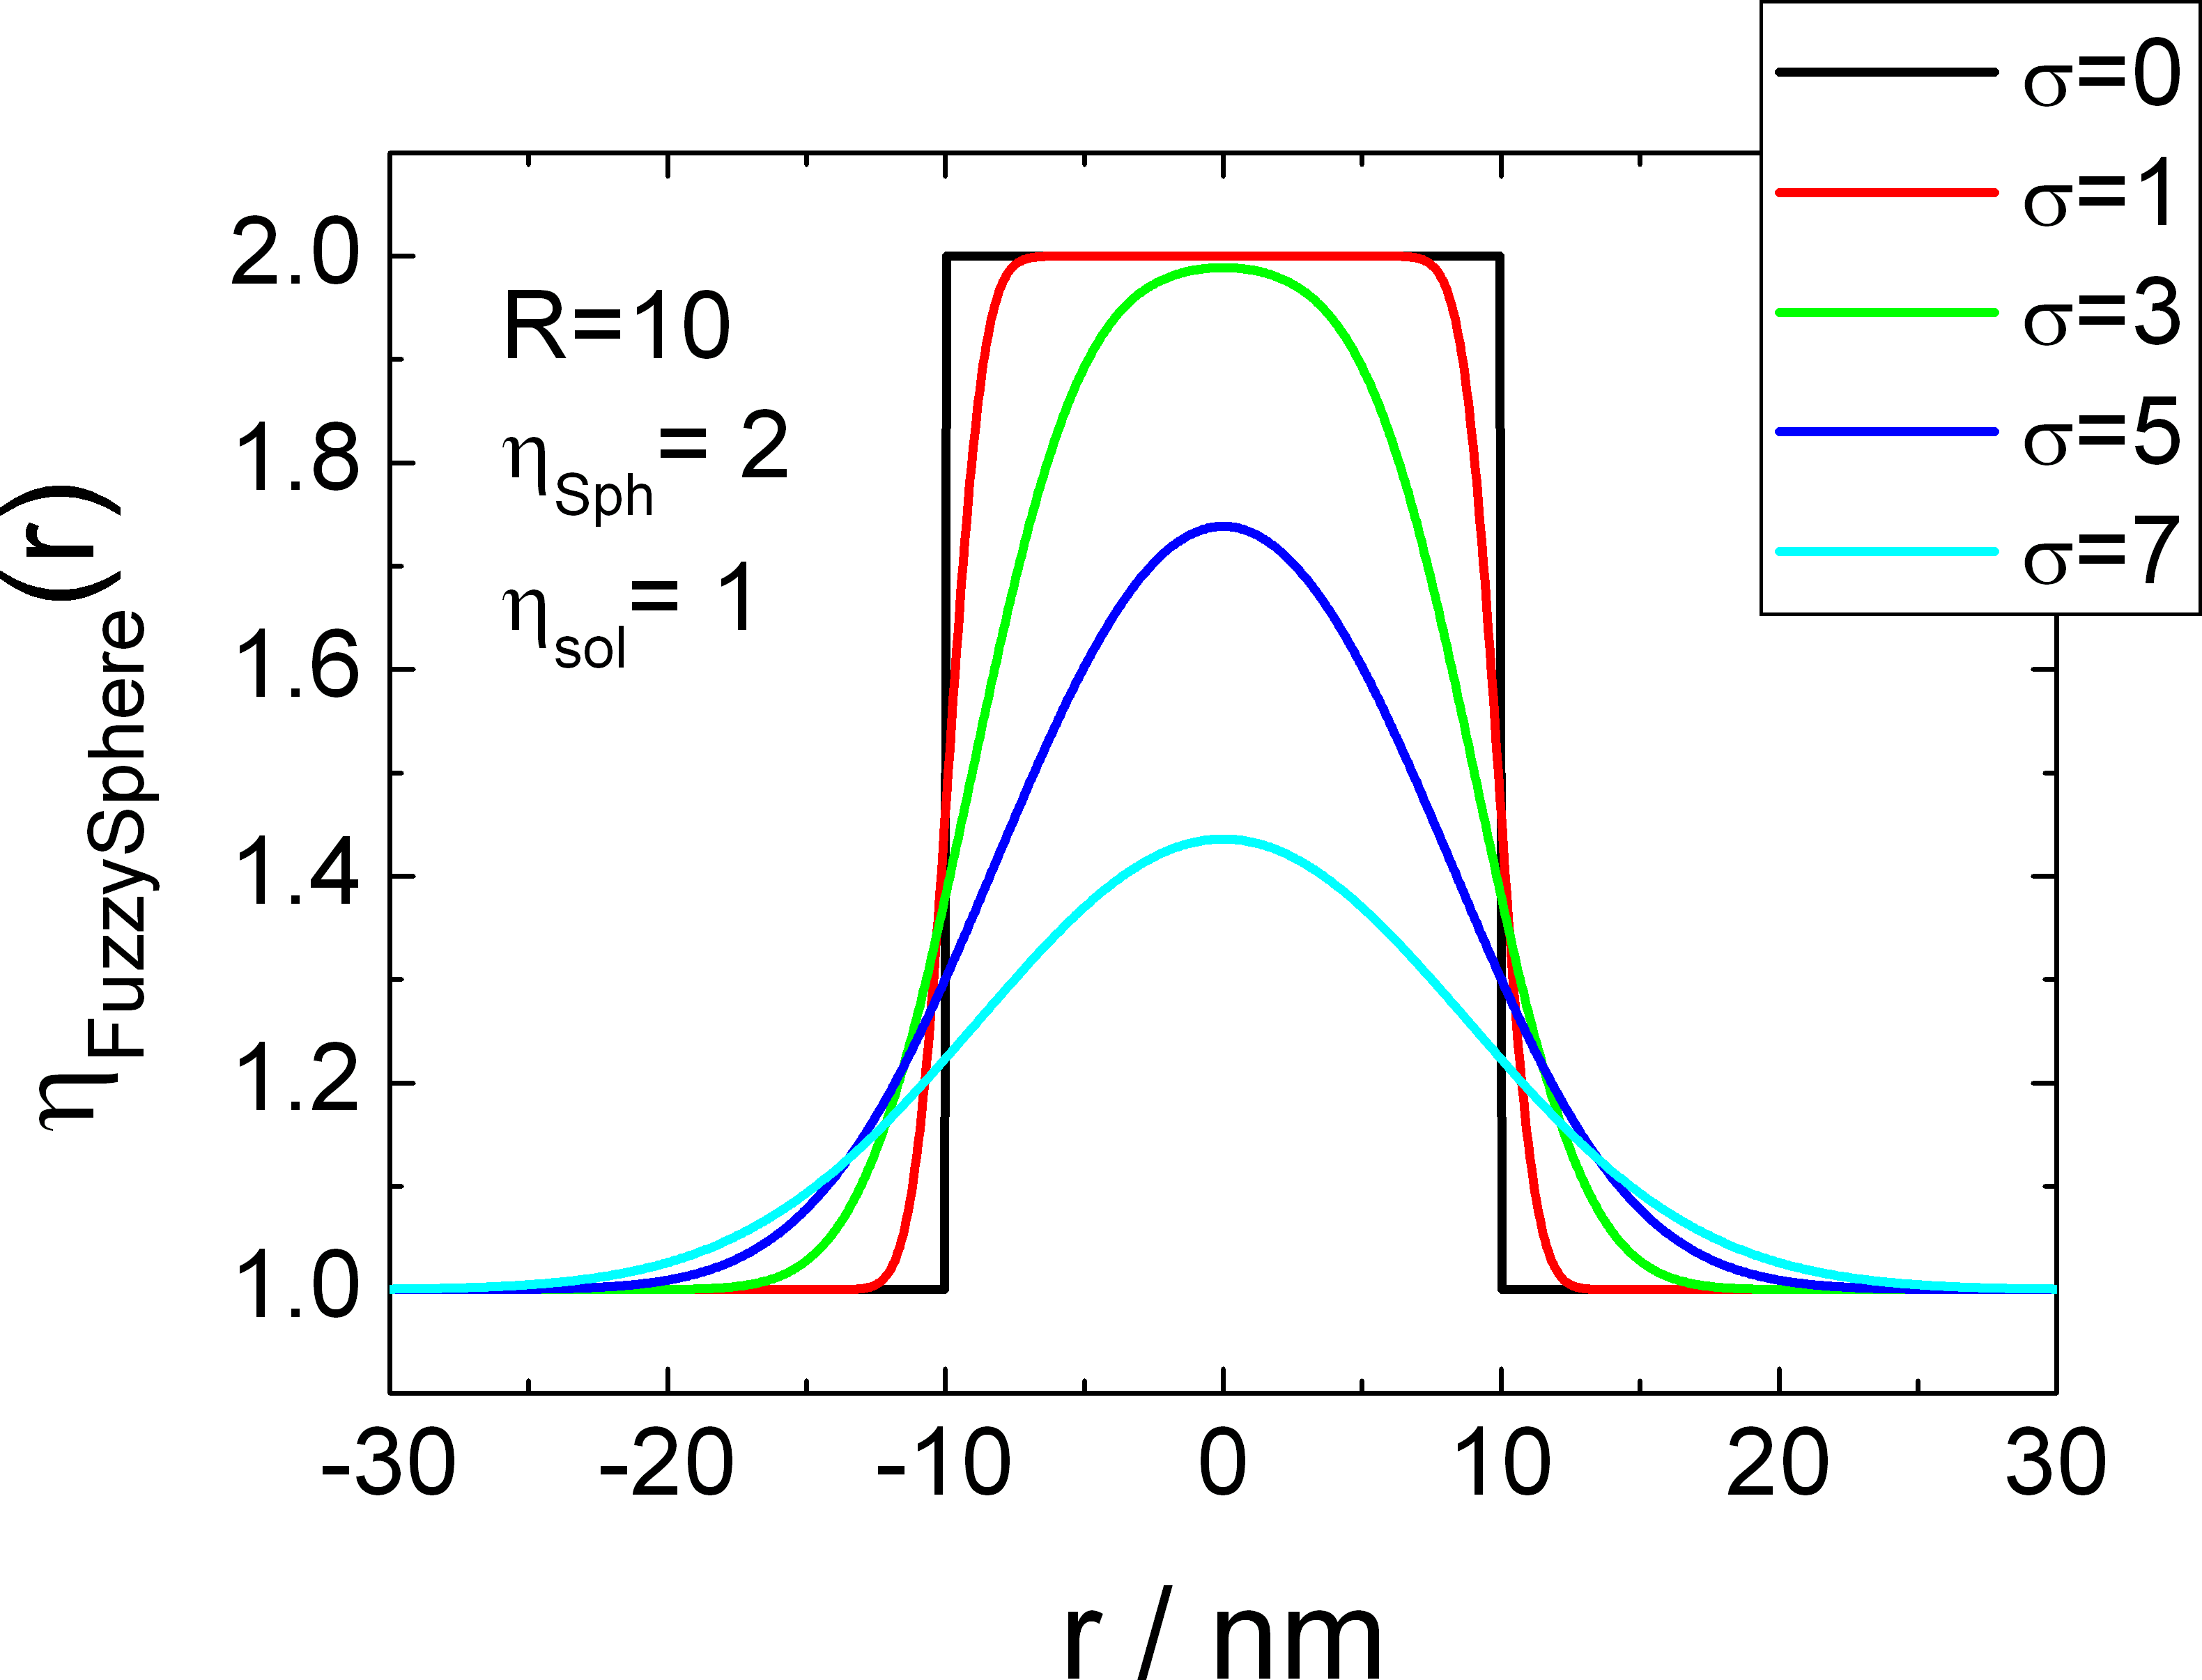
\includegraphics[width=0.7\textwidth,height=0.5\textwidth]{../images/form_factor/FuzzySphere/FuzzySphereProfile.png}
\end{center}
\caption{radial profile of a fuzzy sphere model}
\label{profile:fuzzysphere}
\end{figure}

This model can be used to calculate the scattering from spherical
particles with a "fuzzy" interface \cite{Stieger2004}. The fuzzy
interface is obtained by convoluting the radial profile of a hard
sphere with a Gaussian function.
\begin{align}
\eta_\text{FuzzySph}\left(\abs{\mathbf{r}}\right)
        &= \left(\eta_\text{HS}\star\eta_\text{Gauss}\right)(\mathbf{r}) \nonumber \\
        &= \int_{\mathbb{R}^3}\eta_\text{HS}(\boldsymbol{\tau}) \eta_\text{Gauss}(\mathbf{r}-\boldsymbol{\tau}) d\boldsymbol{\tau}
\end{align}
with
\begin{subequations}
\begin{align}
\eta_\text{HS}\left(\abs{\mathbf{r}}\right) &=
\begin{cases}
\left(\eta_\text{sph}-\eta_\text{sol}\right) & \mbox{for~} \abs{\mathbf{r}}\leq R \\
0 & \mbox{for~} \abs{\mathbf{r}}>R
\end{cases} \\
\eta_\text{Gauss}\left(\abs{\mathbf{r}}\right) &= \frac{1}{2 \sqrt{2} \pi^{3/2}
\abs{\sigma}^3} \exp\left[ -\frac{\abs{\mathbf{r}}^2}{2
\abs{\sigma}^2}\right]
\end{align}
\end{subequations}
The convolution has to be done in $\mathbb{R}^3$. As the hard
sphere and Gaussian functions are radial symmetric also the
profile of the fuzzy sphere only depends on $\abs{\mathbf{r}}$. By
defining the interface via a convolution the form factor can be
easily calculated because the Fourier transform of a convolution
is the pointwise product of the Fourier transforms according to
the convolution theorem, i.e.
\begin{equation}
\begin{split}
F(Q) &= \mathcal{F}\left[\eta_\text{FuzzySph}(r) \right] \\
&=
  \mathcal{F}\left[\left(\eta_\text{HS}\star\eta_\text{Gauss}\right)(r)\right]
= \mathcal{F}\left[\eta_\text{HS}(r)\right] \mathcal{F}\left[\eta_\text{Gauss}(r)\right] \\
%&= \int_0^{\infty} \eta_\text{FuzzySph}(r)\; 4\pi r^2\frac{\sin\left(Qr\right)}{Qr} \; dr \\
&=
   \int_0^{\infty} \eta_\text{HS}(r)\; 4\pi r^2\frac{\sin\left(Qr\right)}{Qr} \; dr \int_0^{\infty} \eta_\text{Gauss}(r)\; 4\pi r^2\frac{\sin\left(Qr\right)}{Qr} \; dr \\
&= \left(\eta_\text{sph}-\eta_\text{sol}\right) 4\pi R^3%8\sqrt{2}\pi^{5/2} R^3
   \frac{\sin\left(QR\right)-QR\cos\left(QR\right)}{\left(QR\right)^3} \quad e^{\left[-\frac{1}{2}\sigma^2Q^2\right]}
\end{split}
\end{equation}

Instead of calculating the convolution integral one also can get
the radial profile of the fuzzy interface by the inverse Fourier
transformation of the scattering amplitude
\begin{align}
\eta_\text{FuzzySph}(r) &= \int_0^{\infty}
\frac{1}{\left(2\pi\right)^3} F(Q) 4\pi Q^2 \frac{\sin\left(Qr\right)}{Qr} \mathrm{d}Q
\end{align}
\begin{multline}
\eta_\text{FuzzySph}(r) = \left(\eta_\text{sph}-\eta_\text{sol}\right) \\
\left( \frac{
    \left(
          e^{-\frac{\left(r + R\right)^2}{2 \sigma^2}}
        - e^{-\frac{\left(r - R\right)^2}{2 \sigma^2}}
    \right) \sigma}{\sqrt{2 \pi} r}
 + \frac{1}{2} \text{erf}\left[\frac{r + R}{\sqrt{2} \abs{\sigma}}\right]
 - \frac{1}{2} \text{erf}\left[\frac{r - R}{\sqrt{2} \abs{\sigma}}\right]
\right)
\end{multline}

Finally the scattering intensity is given by
\begin{multline}
I_\text{FuzzySph}(Q) = F^2(Q) = \\
\left[ \left(\eta_\text{sph}-\eta_\text{sol}\right) 4\pi R^3
   \frac{\sin\left(QR\right)-QR\cos\left(QR\right)}{\left(QR\right)^3} \quad e^{\left[-\frac{1}{2}\sigma^2Q^2\right]}
\right]^2
\end{multline}

The intensity $I_\text{FuzzySph}(Q)$ and also the scattering
length profile $\eta_\text{FuzzySph}(r)$ are normalized so that
\begin{align*}
 \lim_{Q \to \infty} I_\text{FuzzySph}(Q) &= \left( \frac{4}{3}\pi R^3\right)^2 \\
 \int_0^{\infty} 4\pi r^2 \; \eta_\text{FuzzySph}(r) \; \mathrm{d}r &=\frac{4}{3}\pi R^3
\end{align*}

\begin{align}
R &=\text{radius of the fuzzy sphere} \nonumber\\
\sigma &=\text{thickness of the fuzzy shell} \nonumber\\
\eta_\text{sph}   & : \text{scattering length density of sphere} \nonumber \\
\eta_\text{sol}   & : \text{scattering length density of the solvent} \nonumber \\
%I_\text{fluct}    & : \text{forward scattering of the internal fluctuation contribution} \nonumber \\
%\xi               & : \text{correlation length of the fluctuations} \nonumber
\end{align}


\vspace{5mm}

\hspace{1pt}\\
\underline{Input Parameters for model \texttt{FuzzySphere} and \texttt{radial profile of FuzzySphere}:}\\
\begin{description}
\item[\texttt{R}] radius of the fuzzy sphere  $R$
\item[\texttt{sigma}] thickness of the fuzzy shell $\sigma$
\item[\texttt{eta\_sph}] scattering length density of sphere
$\eta_\text{sph}$ \item[\texttt{eta\_sol}] scattering length
density of solvent $\eta_\text{sol}$
%\item[\texttt{I\_fluct}] forward scattering of the internal fluctuation contribution $I_\text{fluct}$
%\item[\texttt{xi}] correlation length of the fluctuations $\xi$
\end{description}

\noindent\underline{Note:}
\begin{itemize}
\item This form factor is only defined for positive radii $R>0$.
\item For $\sigma = 0$ the limiting case of a simple hard sphere
form factor is used.
\item In addition, scattering contributions
arising from fluctuations of the microgel network are often
included in this model expression as a Lorentzian function
\begin{align}
I_\text{fluct}(Q) &= \frac{I_\text{fluct}(0)}{1+\xi^2Q^2}
\end{align}
so that
\begin{align}
I(Q) &= I_\text{FuzzySph}(Q)+I_\text{fluct}(Q)
\end{align}
where $I_\text{fluct}(0)$ is the $Q=0$ limiting intensity and
$\xi$ represents the correlation length of the fluctuations, which
can be considered to be related to the blob or mesh size. It
should be noted that the Lorentzian describes the ensemble average
correlations in the polymer network.

\end{itemize}

\begin{figure}[htb]
\begin{center}
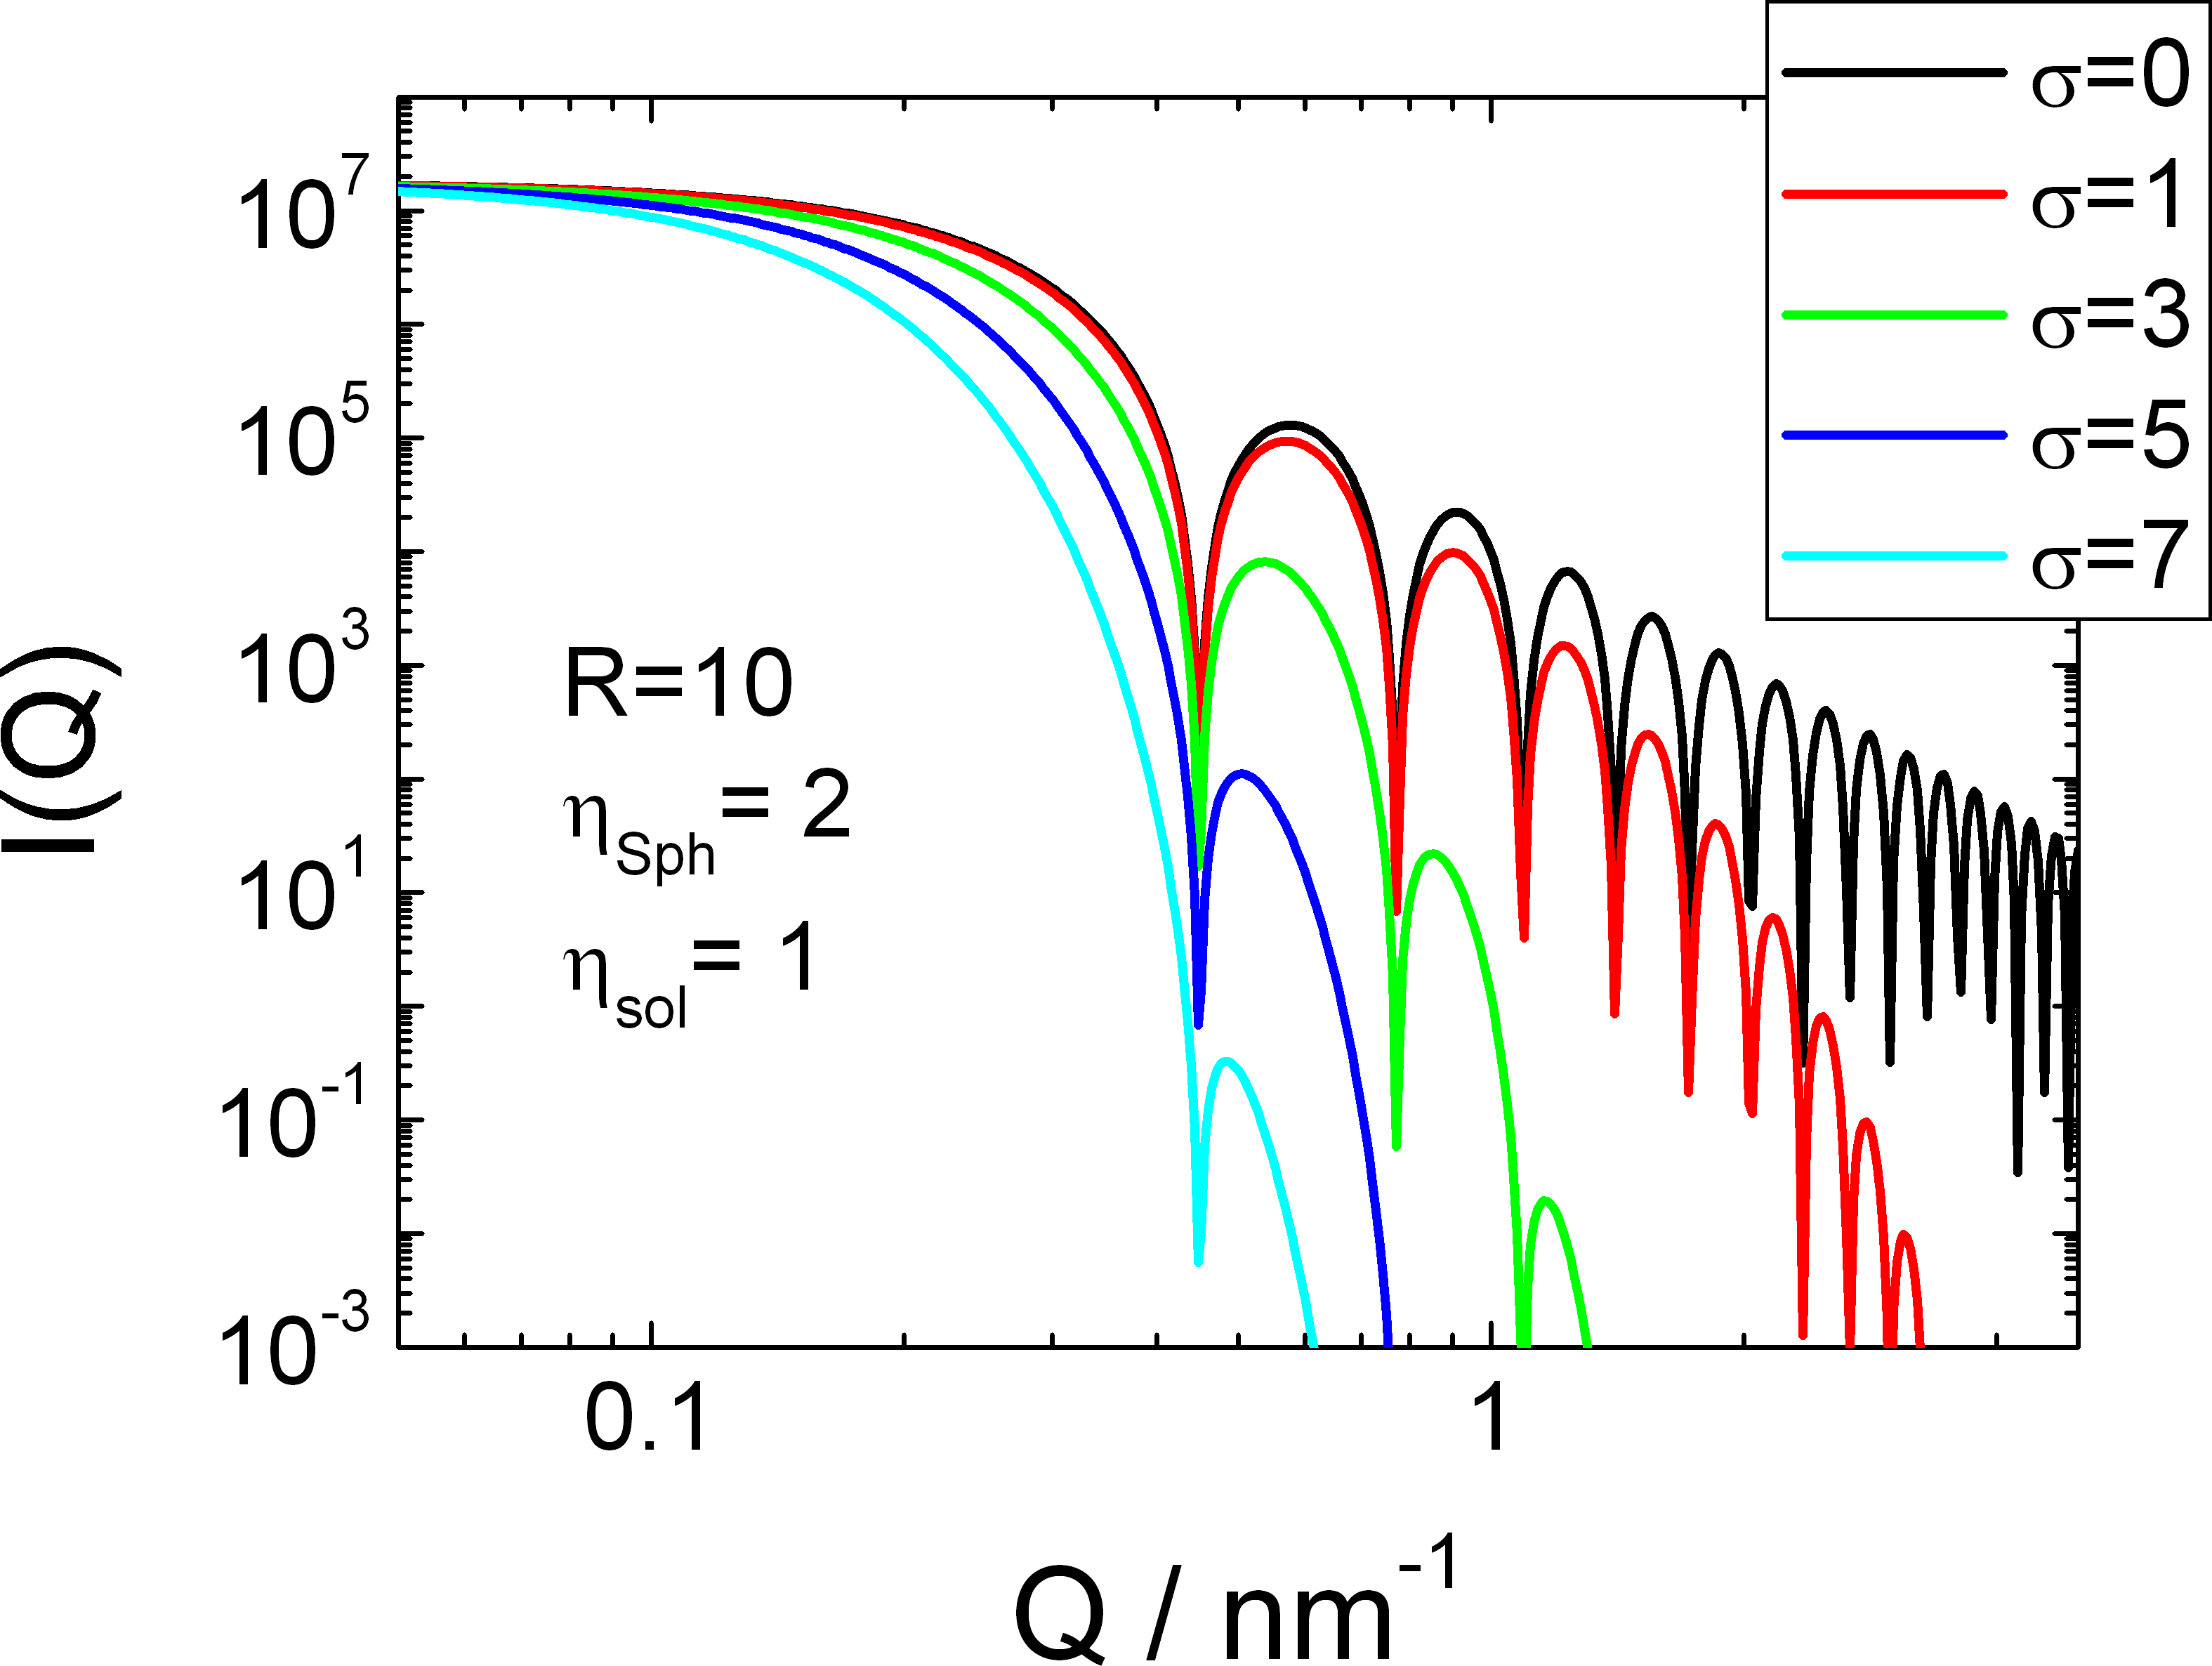
\includegraphics[width=0.7\textwidth,height=0.5\textwidth]{../images/form_factor/FuzzySphere/FuzzySphereIQ.png}
\end{center}
\caption{Scattering intensity of a fuzzy sphere. The scattering
intensity has been calculated for a core radius $R=10$, a
scattering length density of the FuzzySphere of
$\eta_\text{Sph}=1$, a scattering length density of the solvent
$\eta_\text{sol}=1$, and several widths of the "fuzzy" shell}
\label{fig:I_FuzzySphere}
\end{figure}

%%%%%%%%%%%%%%%%%%%%%%%%%%%%%%%%%%%%%%%%%%%%%%%%%%%%%%%%%%%%%%%%%%%%%%%%

\clearpage
\subsection{CoreShellMicrogel}
\label{sect:CoreShellMicrogel}

\begin{figure}[htb]
\begin{center}
\subfigure[radial profile of a sphere with a parabolic interface]{
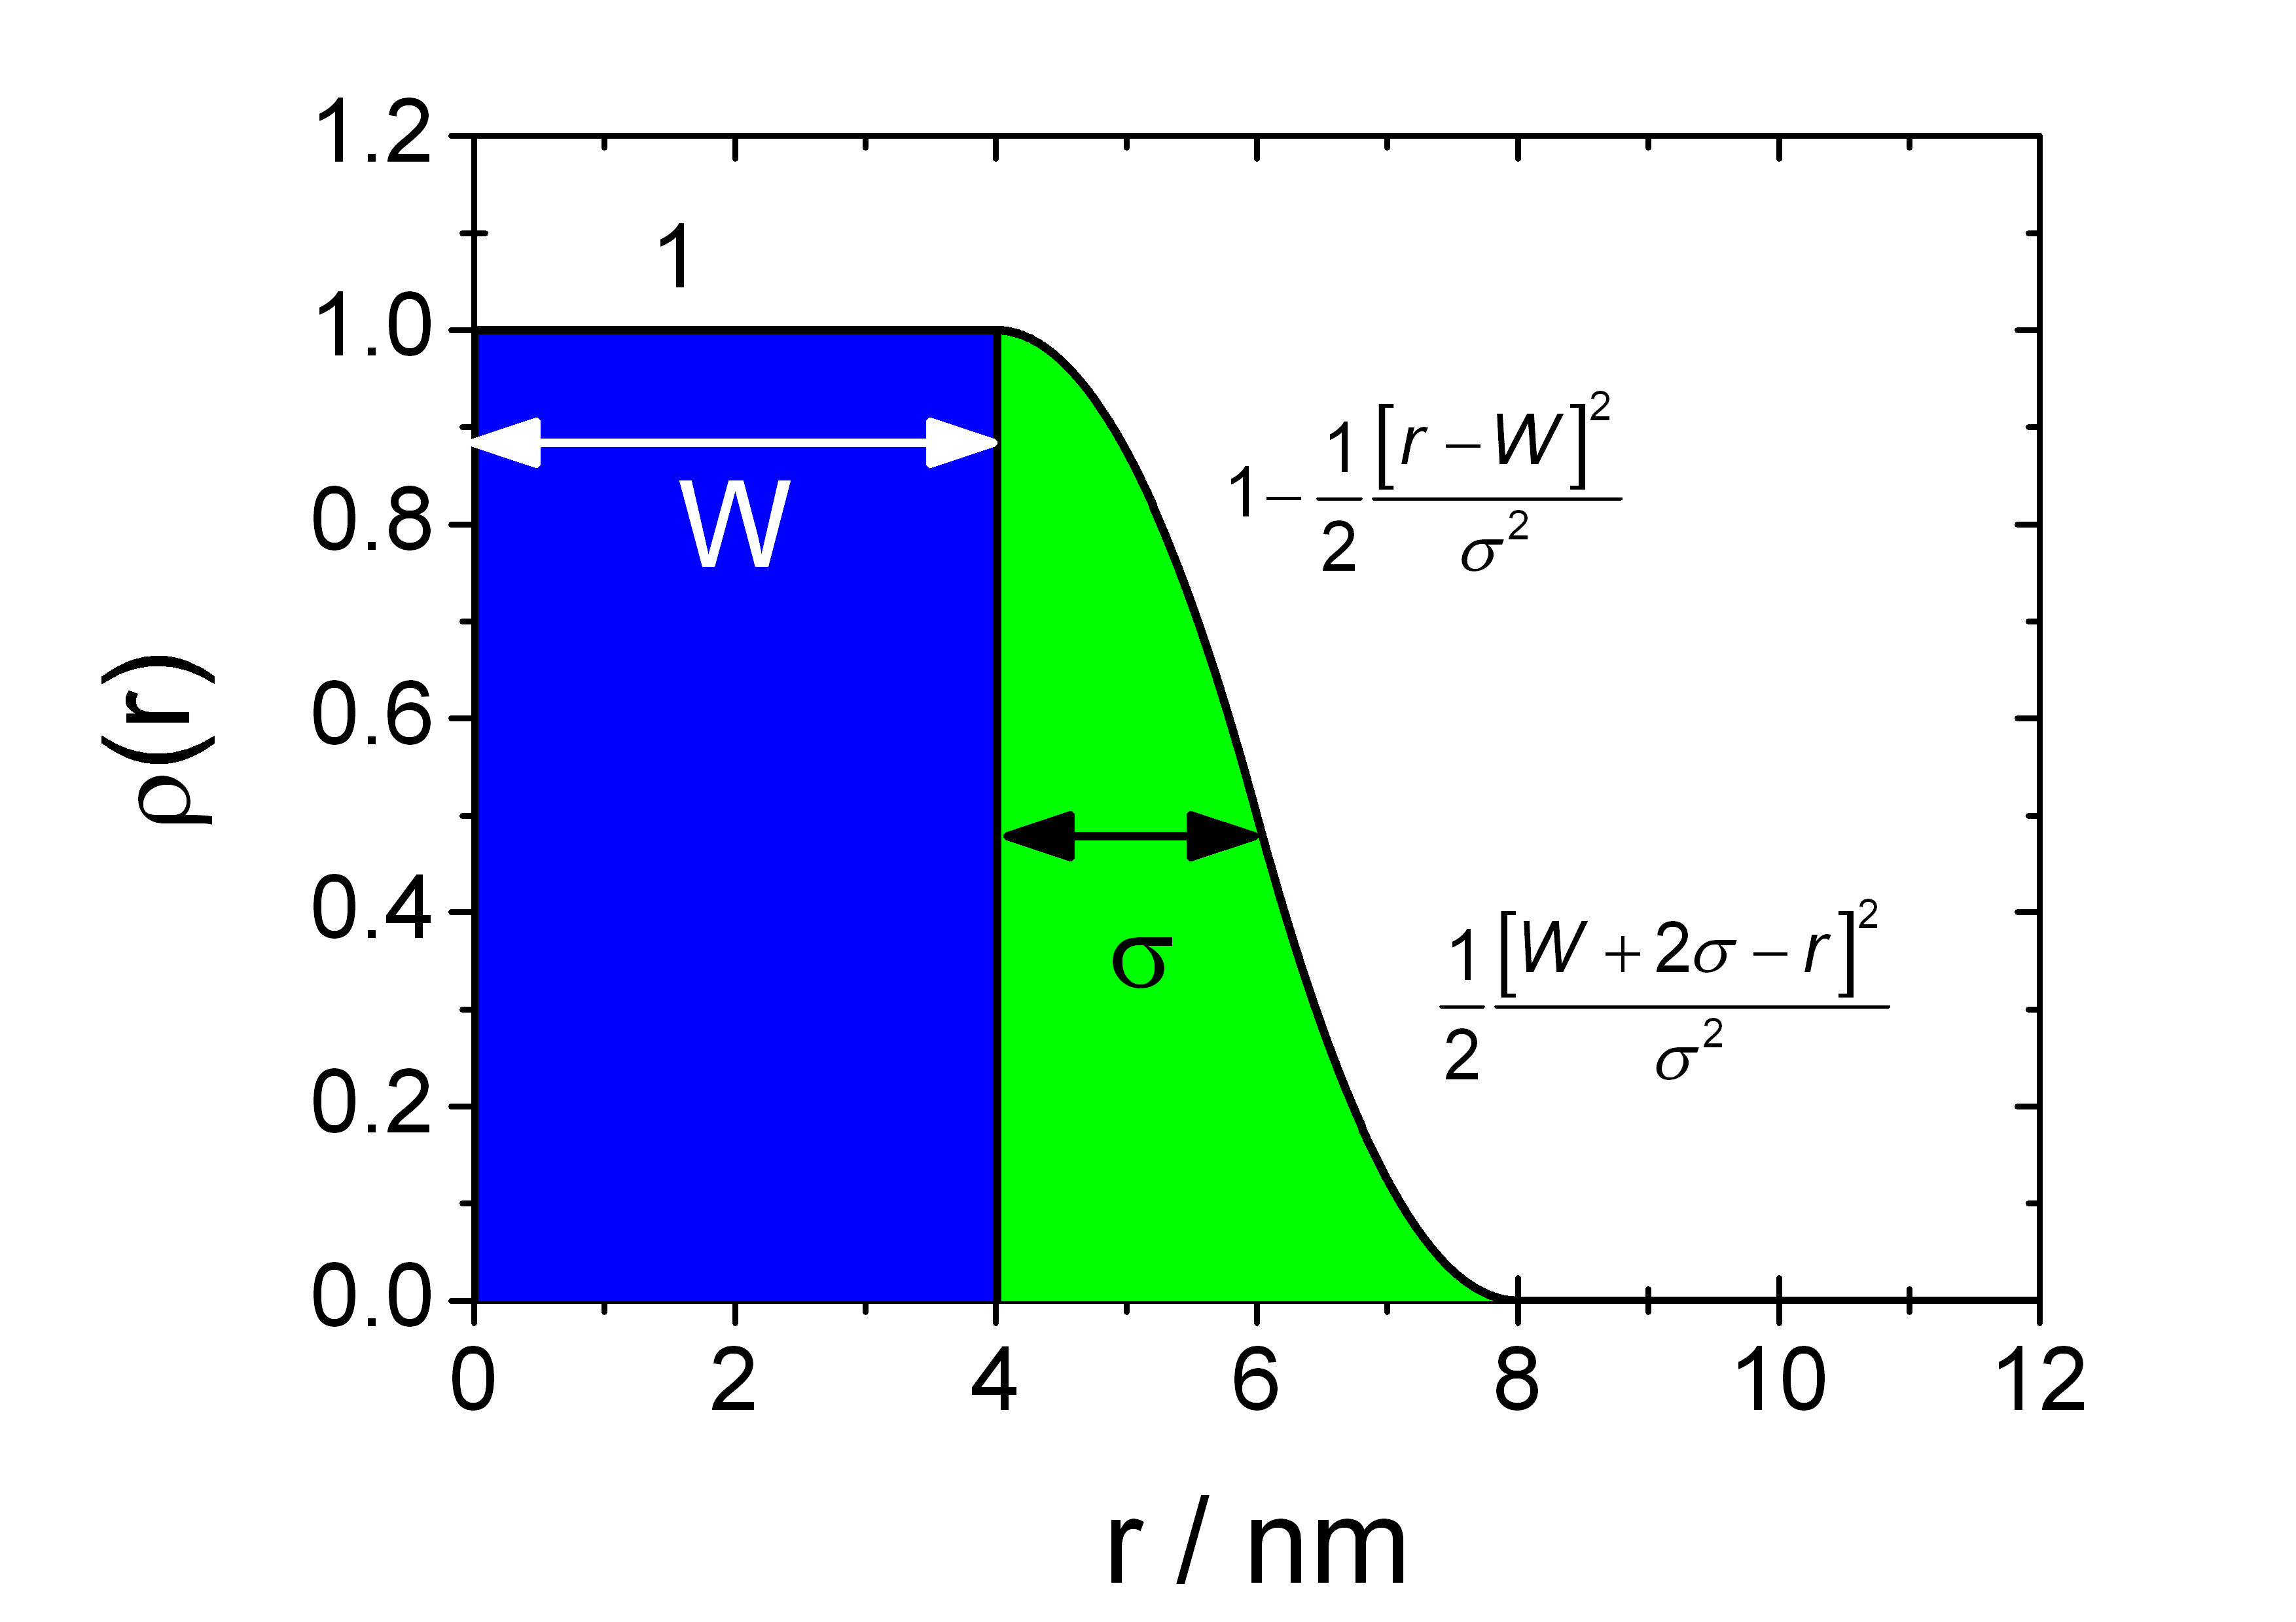
\includegraphics[width=0.48\textwidth,height=0.35\textwidth]{../images/form_factor/FuzzySphere/CoreShellMicrogel1.png}}
\hfill
\subfigure[radial profile of a spherical shell with parabolic interfaces]{
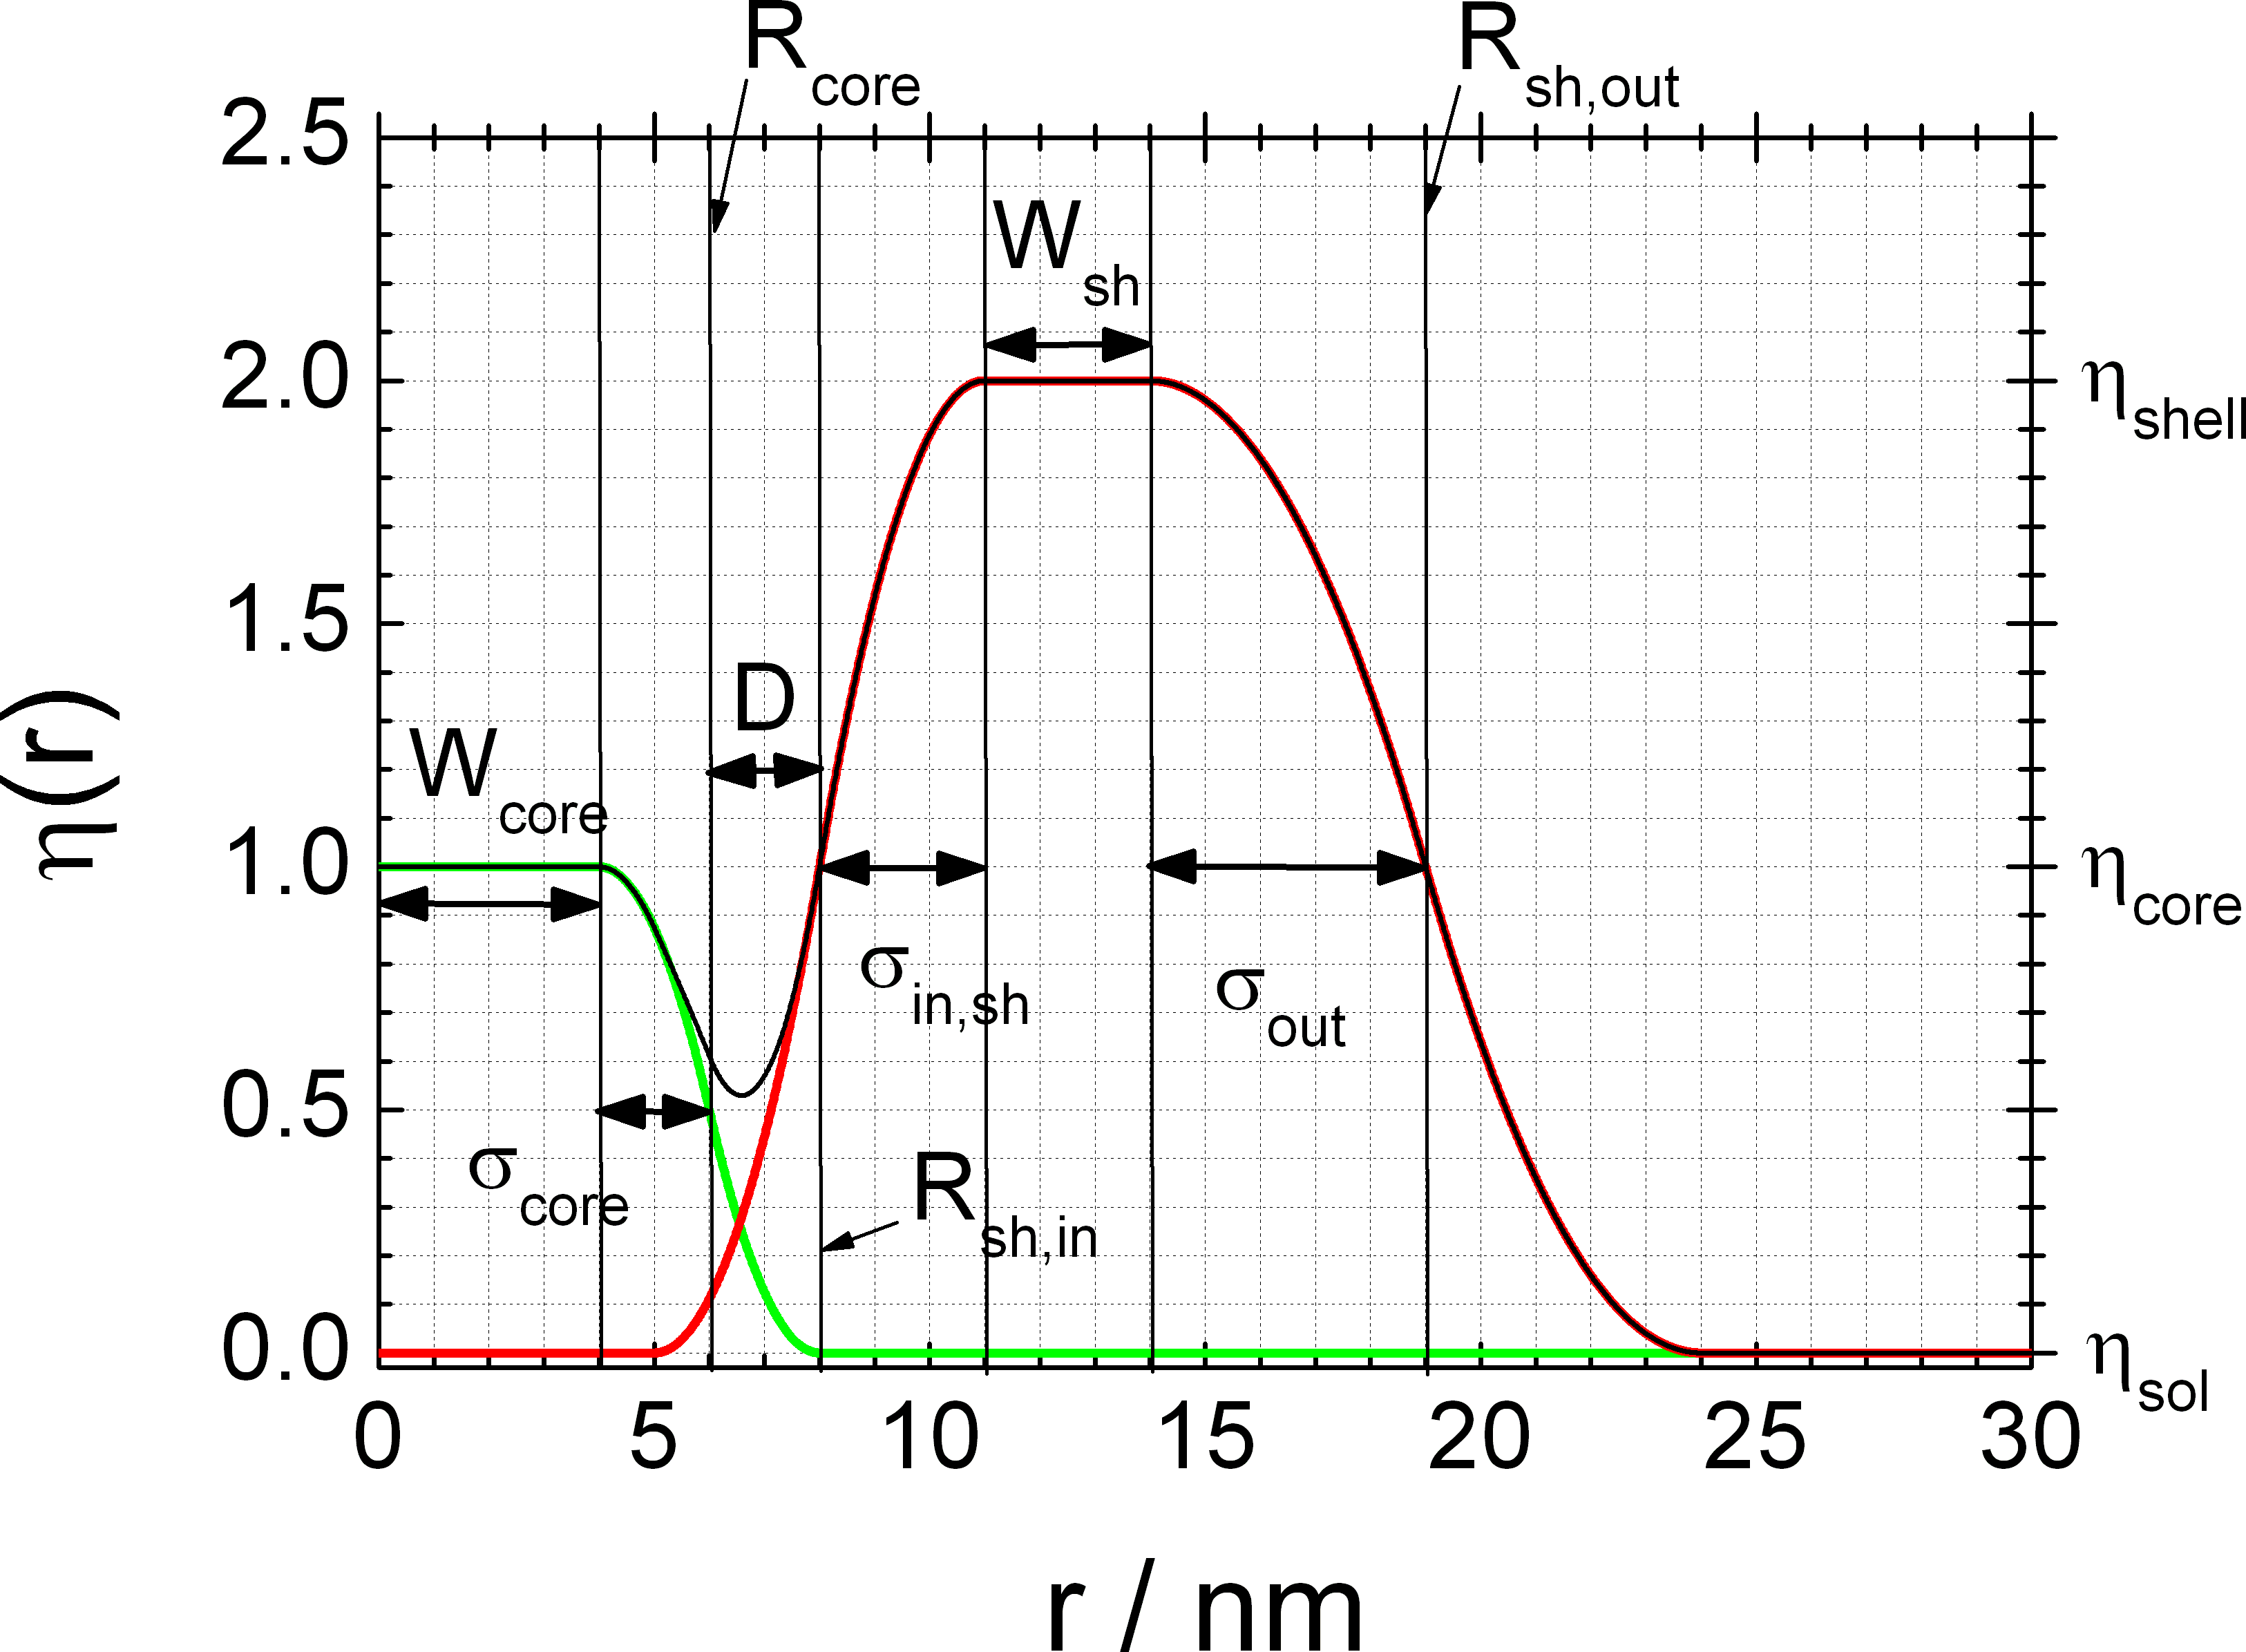
\includegraphics[width=0.48\textwidth,height=0.35\textwidth]{../images/form_factor/FuzzySphere/CoreShellMicrogel2.png}}
\end{center}
\caption{.....}
\label{fig:profile:CoreShellMicrogel}
\end{figure}


This model can be used to calculate the scattering from spherical
particles with a parabolic "fuzzy" interface \cite{Berndt2005,Berndt2006,Berndt2006a}.
The radial profile is given by
\begin{align}
\rho(r,R,\sigma) &=
\begin{cases}
1 & \mbox{for } r\leq R-\sigma \\
1-\frac{1}{2}\frac{\left((r-R)+\sigma\right)^2}{\sigma^2} & \mbox{for } R-\sigma < r \leq R \\
\frac{1}{2}\frac{\left((R-r)+\sigma\right)^2}{\sigma^2} & \mbox{for } R< r\leq R+\sigma \\
0 & \mbox{for } r > \leq R+\sigma
\end{cases}
\label{eq:CoreShellMicrogelProfile}
\end{align}
where $R=W+\sigma$. For such a radial profile the Fourier-transformation can be calculated analytically as
\begin{multline}
F(Q,R,\sigma) = \mathcal{F}[\rho(r,R,\sigma)] = \\
4 \pi \Bigg(
        \left(\frac{R}{\sigma^2}+\frac{1}{\sigma}\right) \frac{\cos (q(R+\sigma))}{q^4}
    +   \left(\frac{R}{\sigma^2}-\frac{1}{\sigma}\right) \frac{\cos (q(R-\sigma))}{q^4} \\
    -   3 \frac{\sin(q(R+\sigma))}{q^5 \sigma^2}
    -   3 \frac{\sin(q(R-\sigma))}{q^5 \sigma^2}
    -   6  \frac{\sin(qR)}{q^5 \sigma^2}
    -   2 R \frac{\cos(qR)}{q^4 \sigma^2}
\Bigg)
\end{multline}
The last term in the brackets needed to be corrected compared to the papers mentioned above
due to a typo in the original papers.
The radial scattering length density profile of a fuzzy core
shell like in Fig.\ \ref{fig:profile:CoreShellMicrogel}b can be obtained by
\begin{multline}
\eta_{core,sh}(r,W_\textrm{core},\sigma_\textrm{core},D,\sigma_\textrm{sh,in},W_\textrm{sh},\sigma_\textrm{sh,out}) =
    \eta_\textrm{sol}
+ (\eta_\textrm{shell}-\eta_\textrm{sol}) \rho(r,R_\textrm{out},\sigma_\textrm{out}) \\
+ (\eta_\textrm{shell}-\eta_\textrm{sol}) \rho(r,R_\textrm{sh,in},\sigma_\textrm{sh,in})
+ (\eta_\textrm{core} -\eta_\textrm{sol}) \rho(r,R_\textrm{core},\sigma_\textrm{core})
\end{multline}
with
\begin{subequations}
\begin{align}
    R_\textrm{core} &= W_\textrm{core}+\sigma_\textrm{core} \\
    R_\textrm{sh,in}&= R_\textrm{core}+D \\
    R_\textrm{out}  &= R_\textrm{sh,in}+\sigma_\textrm{sh,in}+W_\textrm{sh}+\sigma_\textrm{sh,out}
\end{align}
\label{eq:radiiCoreShellMicrogel}
\end{subequations}
In the same way also the scattering amplitude $F_\textrm{core,sh}(Q,\cdots)$ and the scattering intensity
$I_\textrm{core,sh}(Q,\cdots)=\abs{F_\textrm{core,sh}(Q,\cdots)}^2$ can be calculated
\begin{subequations}
\begin{multline}
F_\textrm{core,sh}(Q,W_\textrm{core},\sigma_\textrm{core},D,\sigma_\textrm{sh,in},W_\textrm{sh},\sigma_\textrm{sh,out}) =
  (\eta_\textrm{shell}-\eta_\textrm{sol}) F(Q,R_\textrm{out},\sigma_\textrm{out}) \\
+ (\eta_\textrm{shell}-\eta_\textrm{sol}) F(Q,R_\textrm{sh,in},\sigma_\textrm{sh,in})
+ (\eta_\textrm{core} -\eta_\textrm{sol}) F(Q,R_\textrm{core},\sigma_\textrm{core})
\end{multline}
\begin{align}
I_\textrm{core,sh}(Q,W_\textrm{core},\sigma_\textrm{core},D,\sigma_\textrm{sh,in},W_\textrm{sh},\sigma_\textrm{sh,out}) &=
\abs{F_\textrm{core,sh}(Q,\cdots)}^2
\end{align}
\end{subequations}

\vspace{5mm}

\noindent
\textbf{Input parameters for "\texttt{CoreShellMicrogel}" and "\texttt{radial profile of CoreShellMicrogel}":}
\begin{description}
    \item[\texttt{W\_core}] radius of center parts of core $W_\textrm{core}$ with homogeneous scattering length density
    \item[\texttt{sigma\_core}] interface half width of the core $\sigma_\mathrm{core}$
    \item[\texttt{W\_shell}] width of center parts of shell $W_\textrm{sh}$ with homogeneous scattering length density
    \item[\texttt{sigma\_sh,in}] half width of the inner interface of shell $\sigma_\mathrm{sh,in}$
    \item[\texttt{D}] distance $D$ between interface of core and in interface of shell
    \item[\texttt{sigma\_out}] half width of the outer surface profile $\sigma_\mathrm{out}$
    \item[\texttt{eta\_core}] scattering length density of homogeneous core part $\eta_\textrm{core}$
    \item[\texttt{eta\_shell}] scattering length density of homogeneous shell part $\eta_\textrm{shell}$
    \item[\texttt{eta\_sol}] scattering length density of solvent $\eta_\textrm{sol}$
\end{description}

\noindent
\textbf{Note}
\begin{itemize}
  \item If one like to simulate a simple step profile one should set $D=0$ and
        $\sigma_\mathrm{core}=\sigma_\mathrm{sh,in}$. The last equality
        in case of fitting this parameter can be simply obtained by a global parameter
        under fitting multiple data sets.
  \item Instead of using the radii in eq.\ \ref{eq:radiiCoreShellMicrogel} as input parameters the thickness
        of the homogeneous parts of the core and the shell have been used to avoid a problems
        (negative dimensions) by applying an integration over a size distribution starting from 0 on the radii.
\end{itemize}
\begin{figure}[htb]
\begin{center}
\subfigure[Some radial profiles of spheres with a parabolic interfaces  which have been used to calculate the scattering curve in Fig.\ (b).
]{
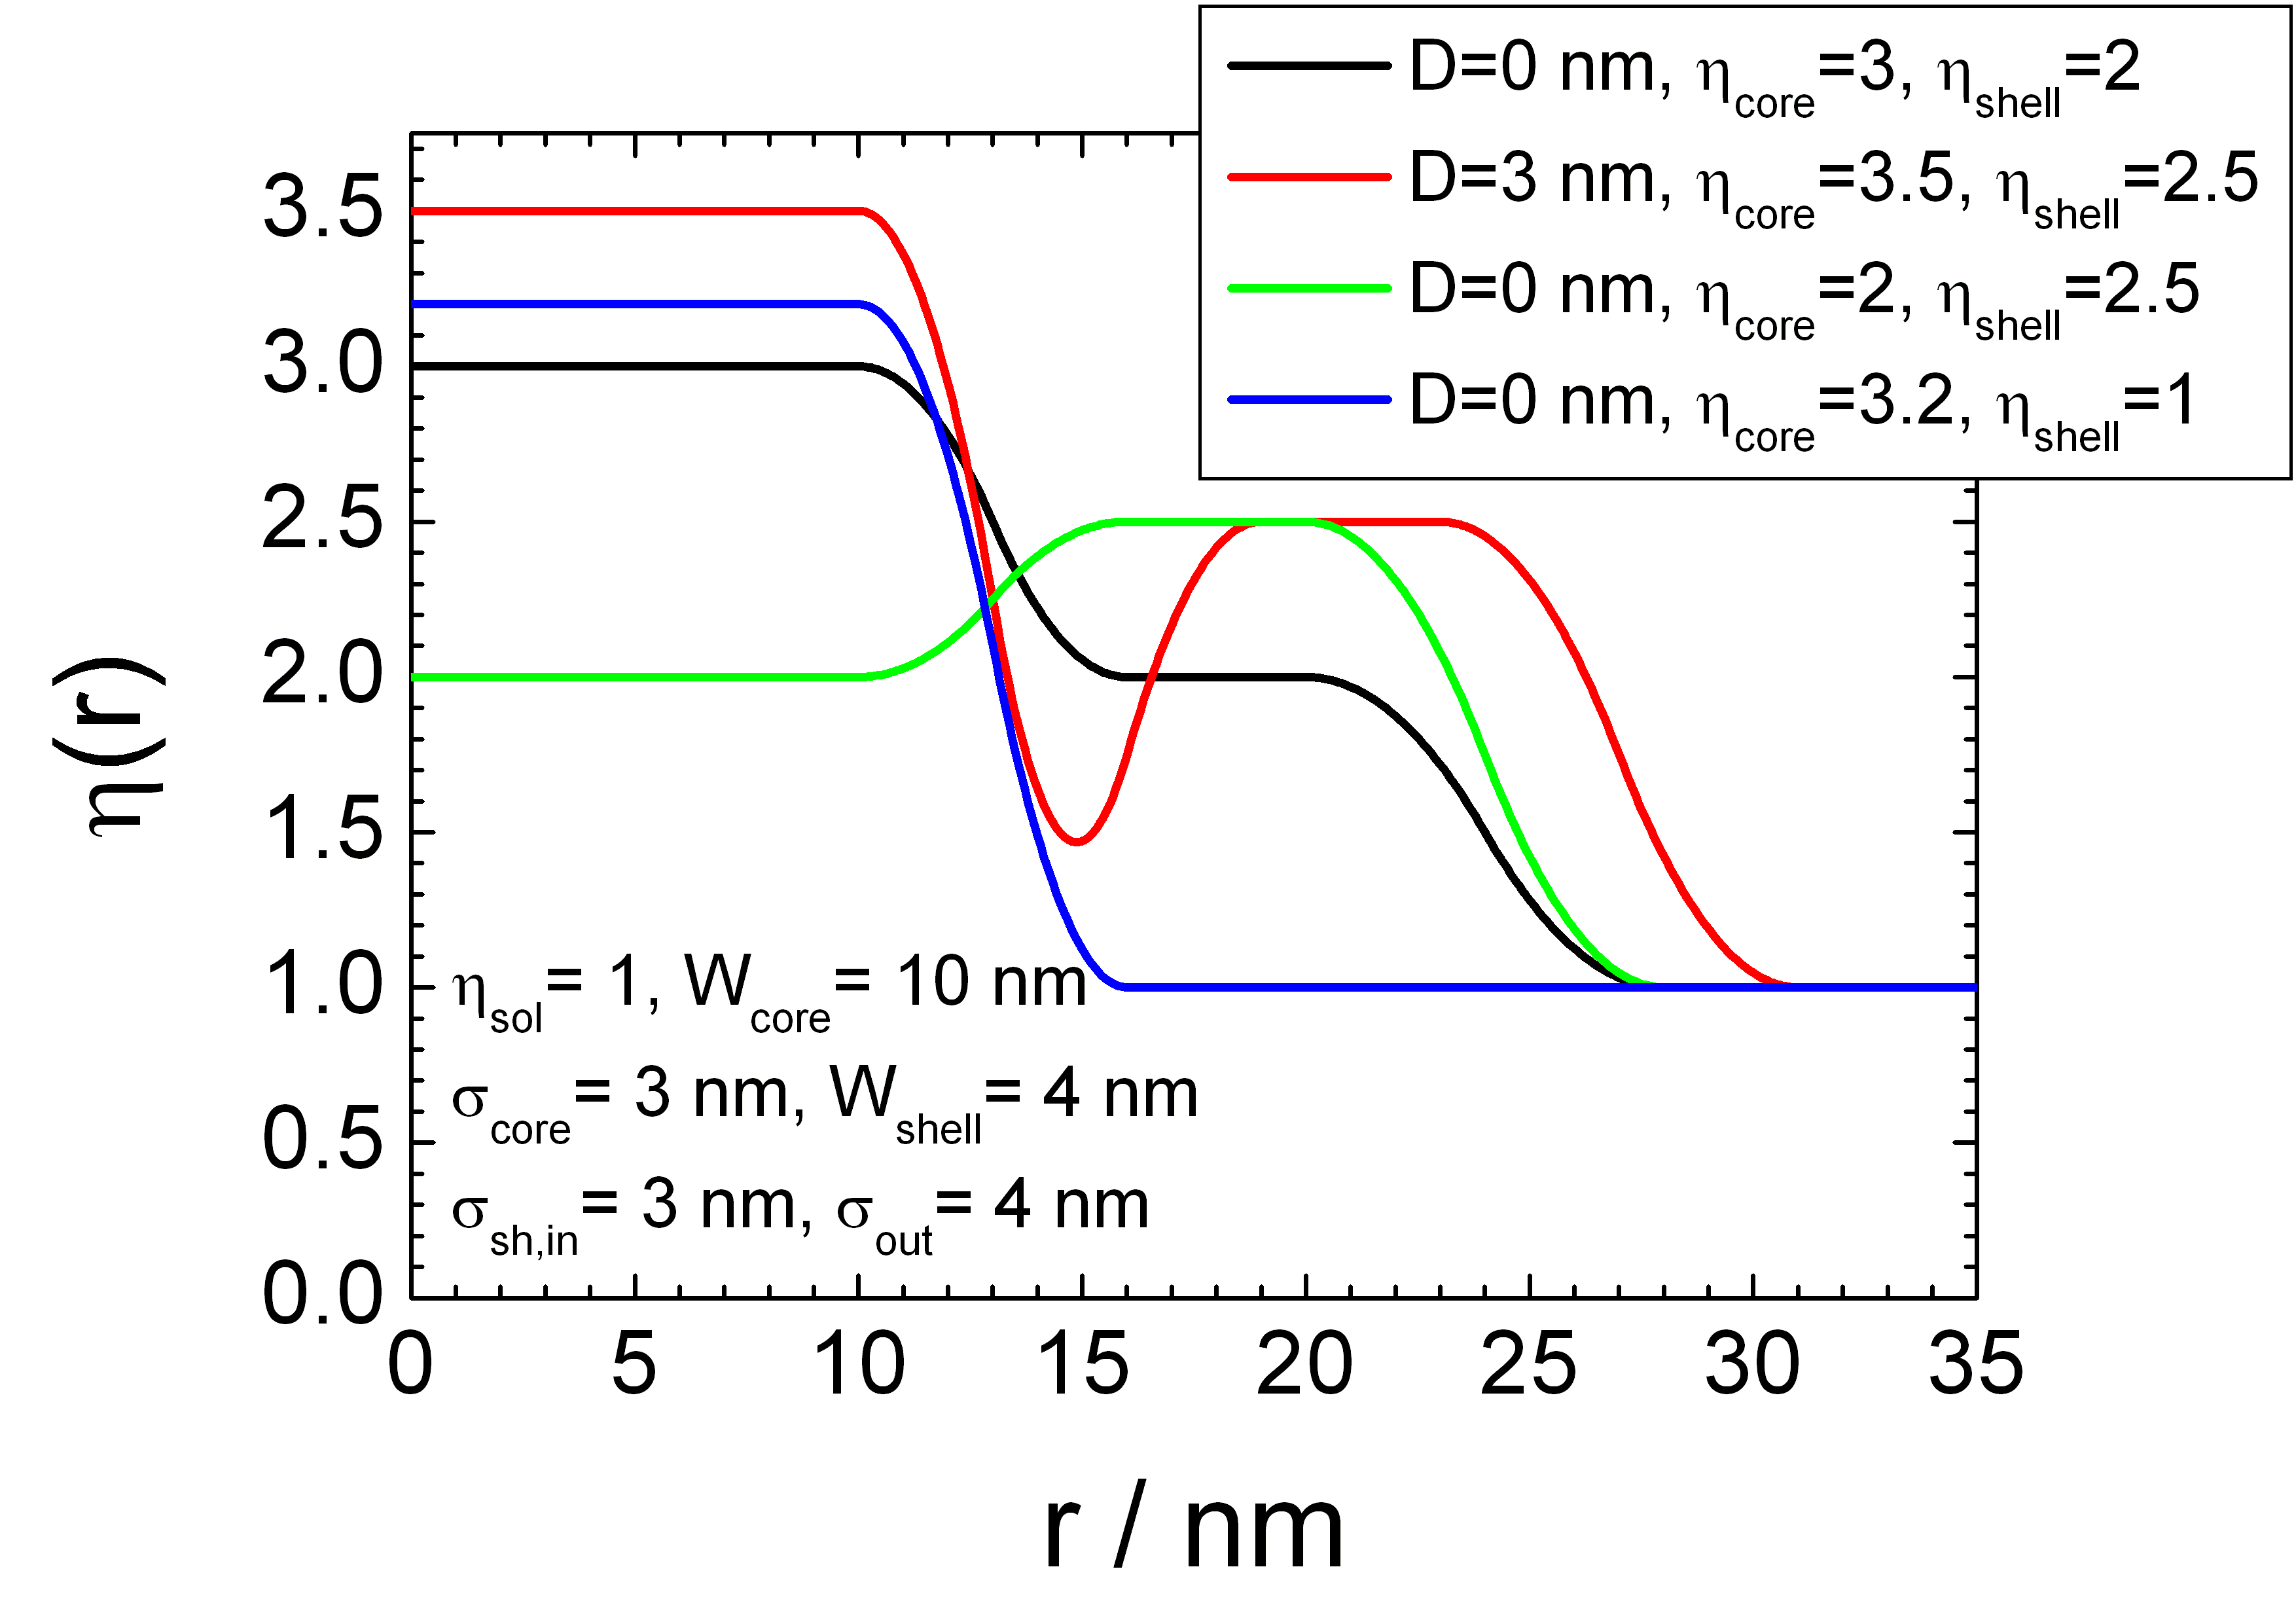
\includegraphics[width=0.48\textwidth,height=0.35\textwidth]{../images/form_factor/FuzzySphere/Example_CoreShellMicrogel1.png}}
\hfill
\subfigure[Scattering curves of the radial profiles shown in Fig.\ (a).]{
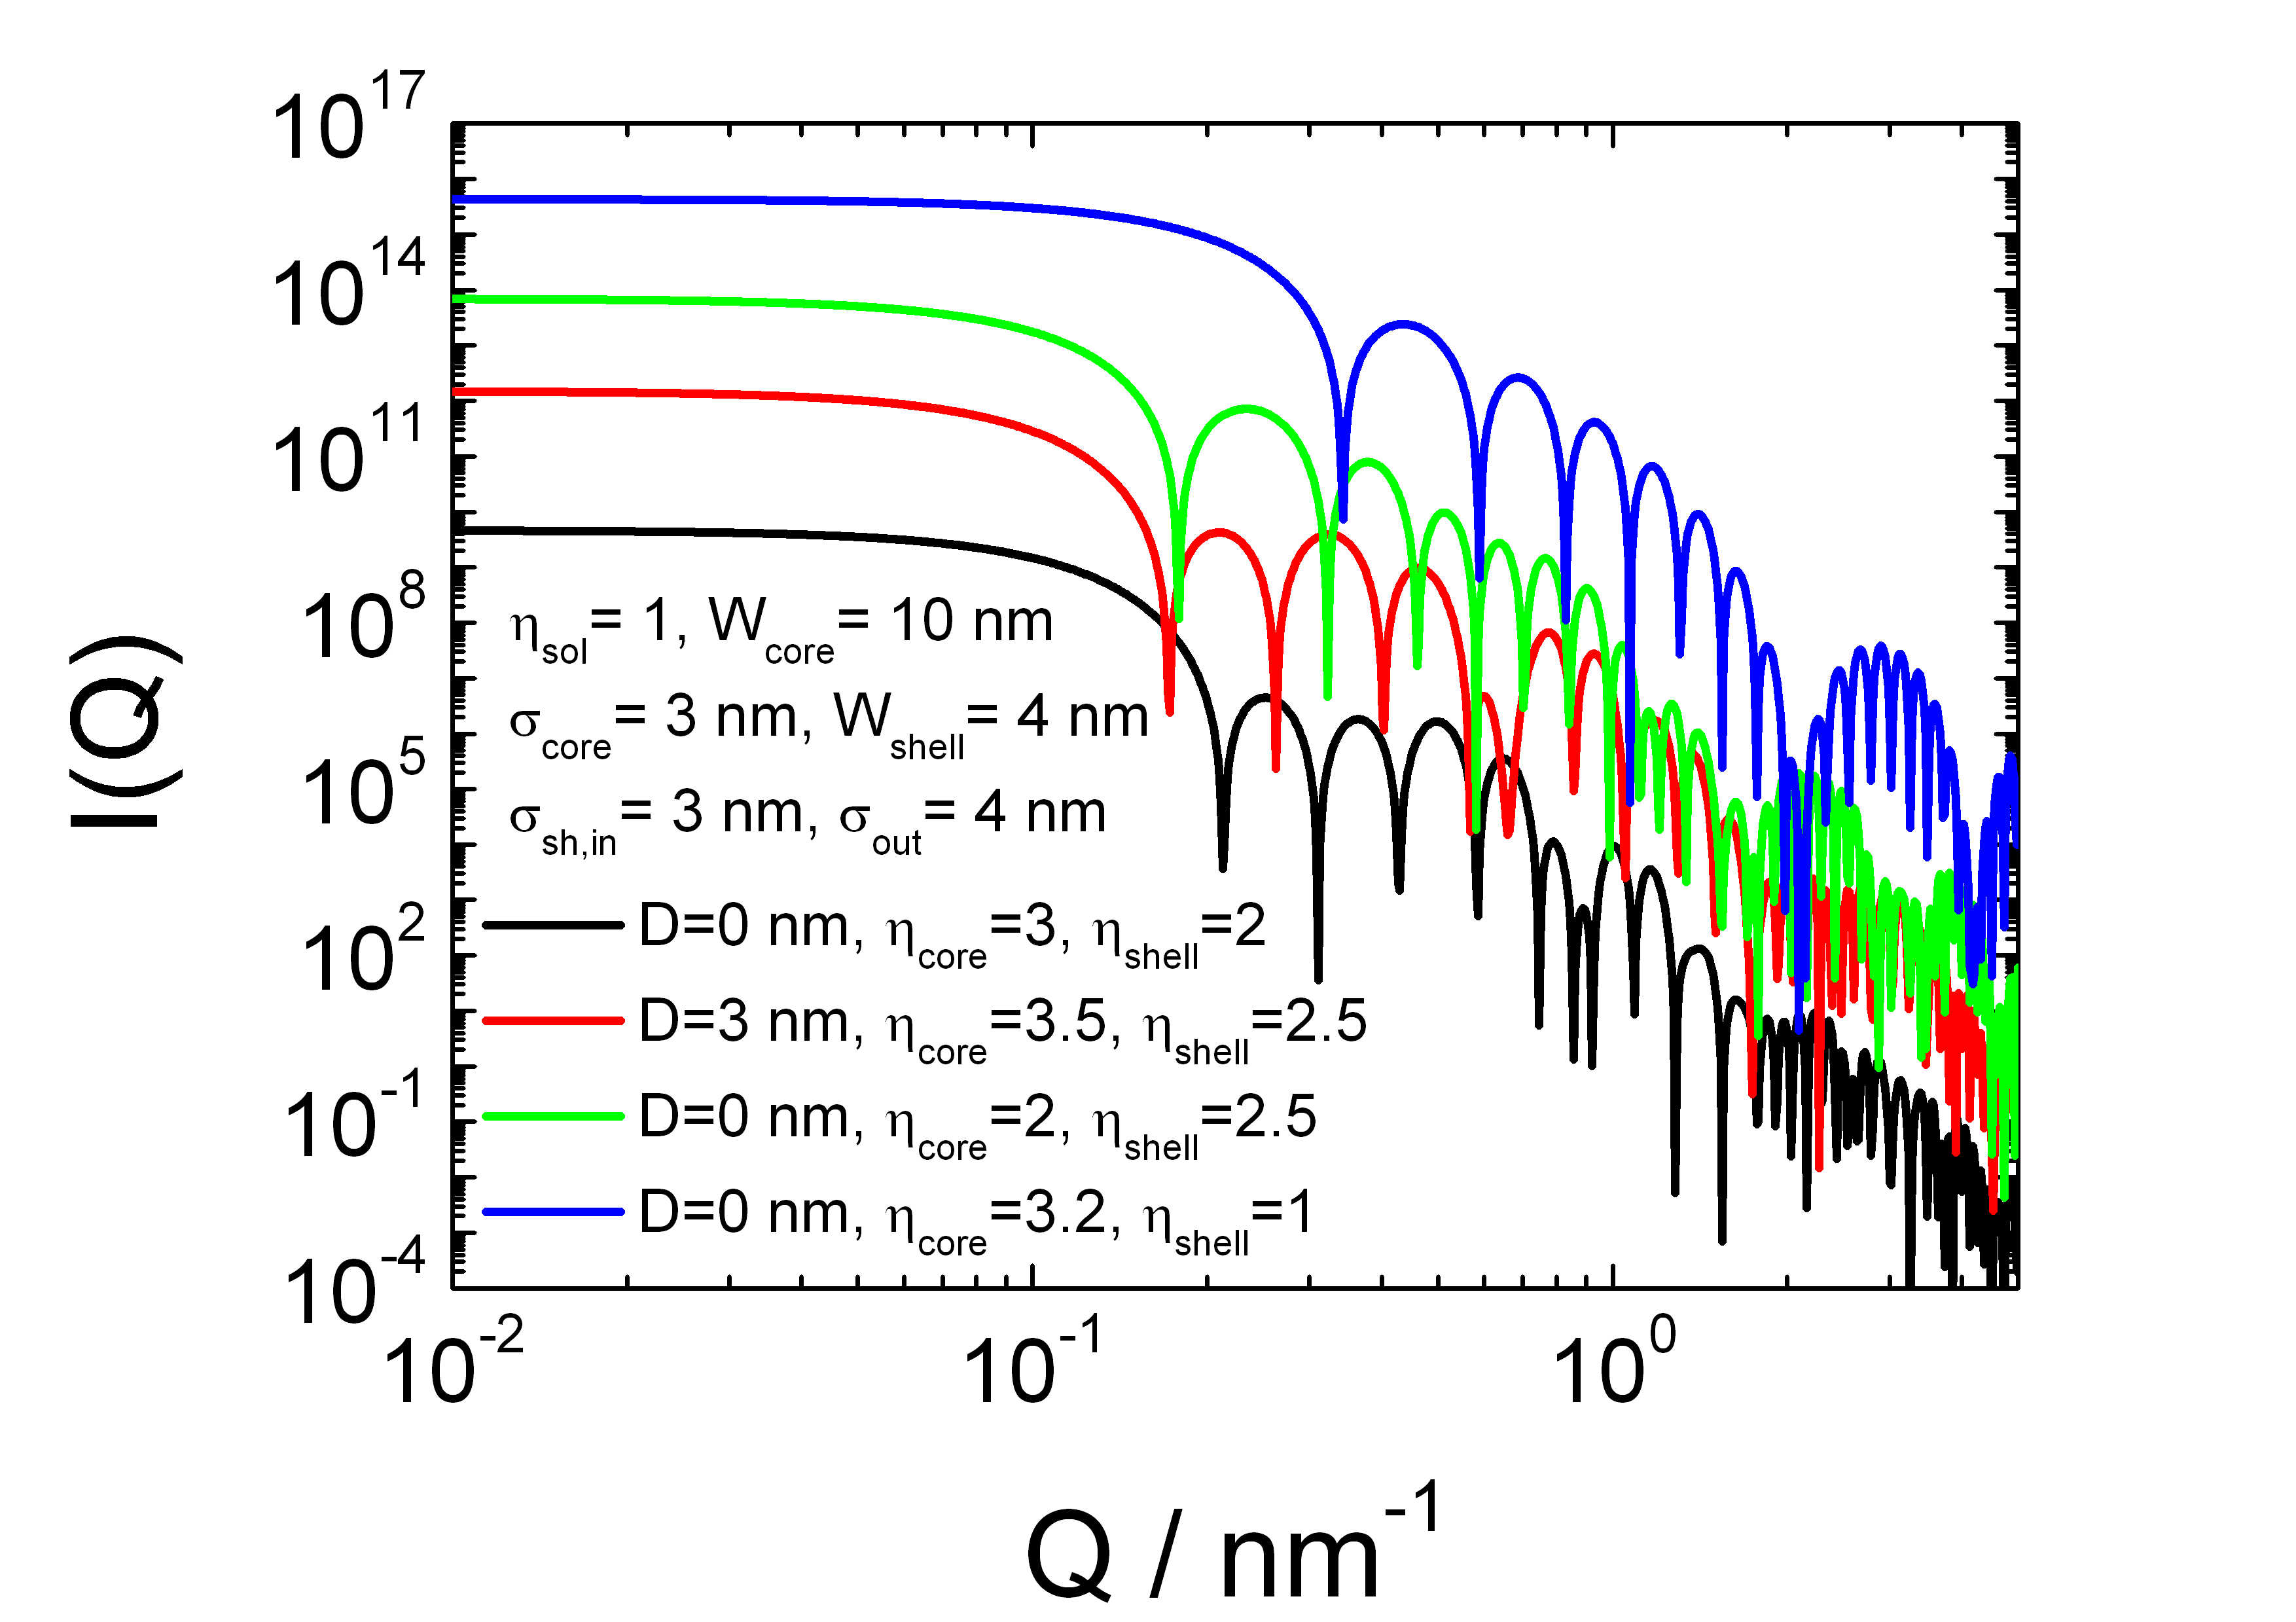
\includegraphics[width=0.48\textwidth,height=0.35\textwidth]{../images/form_factor/FuzzySphere/Example_CoreShellMicrogel2.png}}
\end{center}
\caption{The profiles and scattering curves hve been calculated with the plugin functions
"\texttt{CoreShellMicrogel}" and "\texttt{Radial Profile of CoreShellMicrogel}".}
\label{fig:profile:Example_CoreShellMicrogel}
\end{figure}

%%%%%%%%%%%%%%%%%%%%%%%%%%%%%%%%%%%%%%%%%%%%%%%%%%%%%%%%%%%%%%%%%%%%%%%%%%%%%%%%

\clearpage
\subsubsection{Spherical shell with linear varying contrast profile (LinShell)}
\label{sect:LinShell} ~\\

\begin{figure}[htb]
\begin{center}
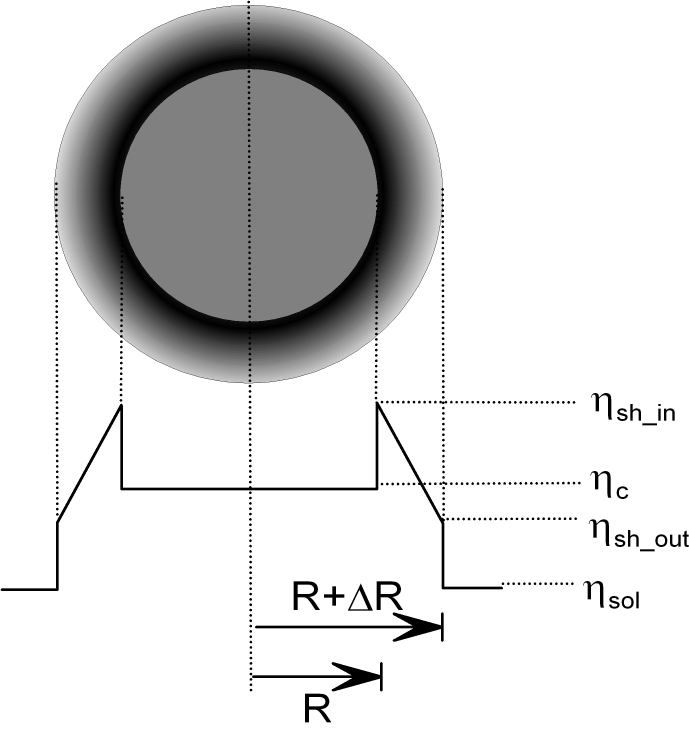
\includegraphics[width=0.5\textwidth,height=0.533\textwidth]{../images/form_factor/spheres/linshell.png}
\end{center}
\caption{Radial profile for calculating the form factor of a spherical shell with a core radius $R$
and a shell thickness of $\Delta R$ and a linear varying contrast
profile.} \label{LinShell1Profile}
\end{figure}

Form factor of a spherical shell with a core radius $R$ and a
shell thickness of $\Delta R$. Here a linear contrast profile
within the shell has been assumed.

\begin{align}
\Delta\eta(r)      & =
\begin{cases}
\eta_\text{c} & \text{~for~} r<R \\
m r + b  & \text{~for~} r \in [R,R+\Delta R] \\
\eta_\text{sol}  & \text{~for~} r>R+\Delta R
\end{cases}\\
m           & = (\eta_\text{sh\_out}-\eta_\text{sh\_in}) / \Delta R \\
b           & = -m R + \eta_\text{sh\_in} \\
\eta_\text{sh\_in}  & = (1 - x_\text{in,sol})  \, \eta_\text{sh} + x_\text{in,sol} \,\eta_\text{sol}-\eta_\text{sol} \\
                    & : \text{scattering length density at $R$} \nonumber \\
\eta_\text{sh\_out} & = (1 - x_\text{out,sol}) \, \eta_\text{sh} + x_\text{out,sol}\,\eta_\text{sol}-\eta_\text{sol} \\
                    & : \text{scattering length density at $R+\Delta R$} \nonumber \\
\eta_\text{sh}      & : \text{scattering length density of pure shell material} \nonumber \\
\eta_\text{c}       & : \text{scattering length density of core} \nonumber \\
\nonumber
\end{align}

\begin{align}
F_\text{sph}(A,x) & = \frac{4}{3}\pi x^3 \,\, 3\frac{\sin(A)-A\cos(A)}{A^3} \\[5mm]
F_\text{shlin}(A,x) & = 4\pi x^4 \frac{2\cos(A)+2A\sin(A)-A^2\cos(A)}{A^4} \\[5mm]
I_\text{LinShell}    & = \big[ \,\, (\eta_\text{c}-\eta_\text{sol}-b)F_\text{sph}(QR,R) \nonumber \\
             & \hspace{6mm} - mF_\text{shlin}(QR,R) \\
             & \hspace{6mm} + mF_\text{shlin}\left(Q(R+\Delta R),R+\Delta R\right) \nonumber \\
             & \hspace{6mm} + bF_\text{sph}\left(Q(R+\Delta R),R+\Delta R\right) \big]^2 \nonumber
\end{align}

\vspace{5mm}

\underline{Input Parameters for model \texttt{LinShell} and \texttt{radial profile of LinShell}:}\\
\begin{description}
\item[\texttt{R}] radius of core $R$
\item[\texttt{dR}] thickness of the shell $\Delta R$
\item[\texttt{eta\_c}] scattering length density $\eta_\text{c}$
\item[\texttt{eta\_sh}] scattering length density of non-swollen shell $\eta_\text{sh}$
\item[\texttt{x\_in}] amount of solvent $x_\text{in,sol}$ on core-shell interface at $R$
\item[\texttt{x\_out}] amount of solvent $x_\text{out,sol}$ on shell-solvent interface at $R+\Delta R$
\item[\texttt{eta\_sol}] scattering length density of solvent $\eta_\text{sol}$
\end{description}

\noindent\underline{Note:}
\begin{itemize}
\item $x_\text{in,sol}$ and $x_\text{out,sol}$ are only physical for values between 0 and 1.
\end{itemize}


\begin{figure}[htb]
\begin{center}
\subfigure[Some radial profiles of spheres with a linear interface profiles
due to penetration of solvent into the shell which have been used to calculate
the scattering curve in Fig.\ (b).]{
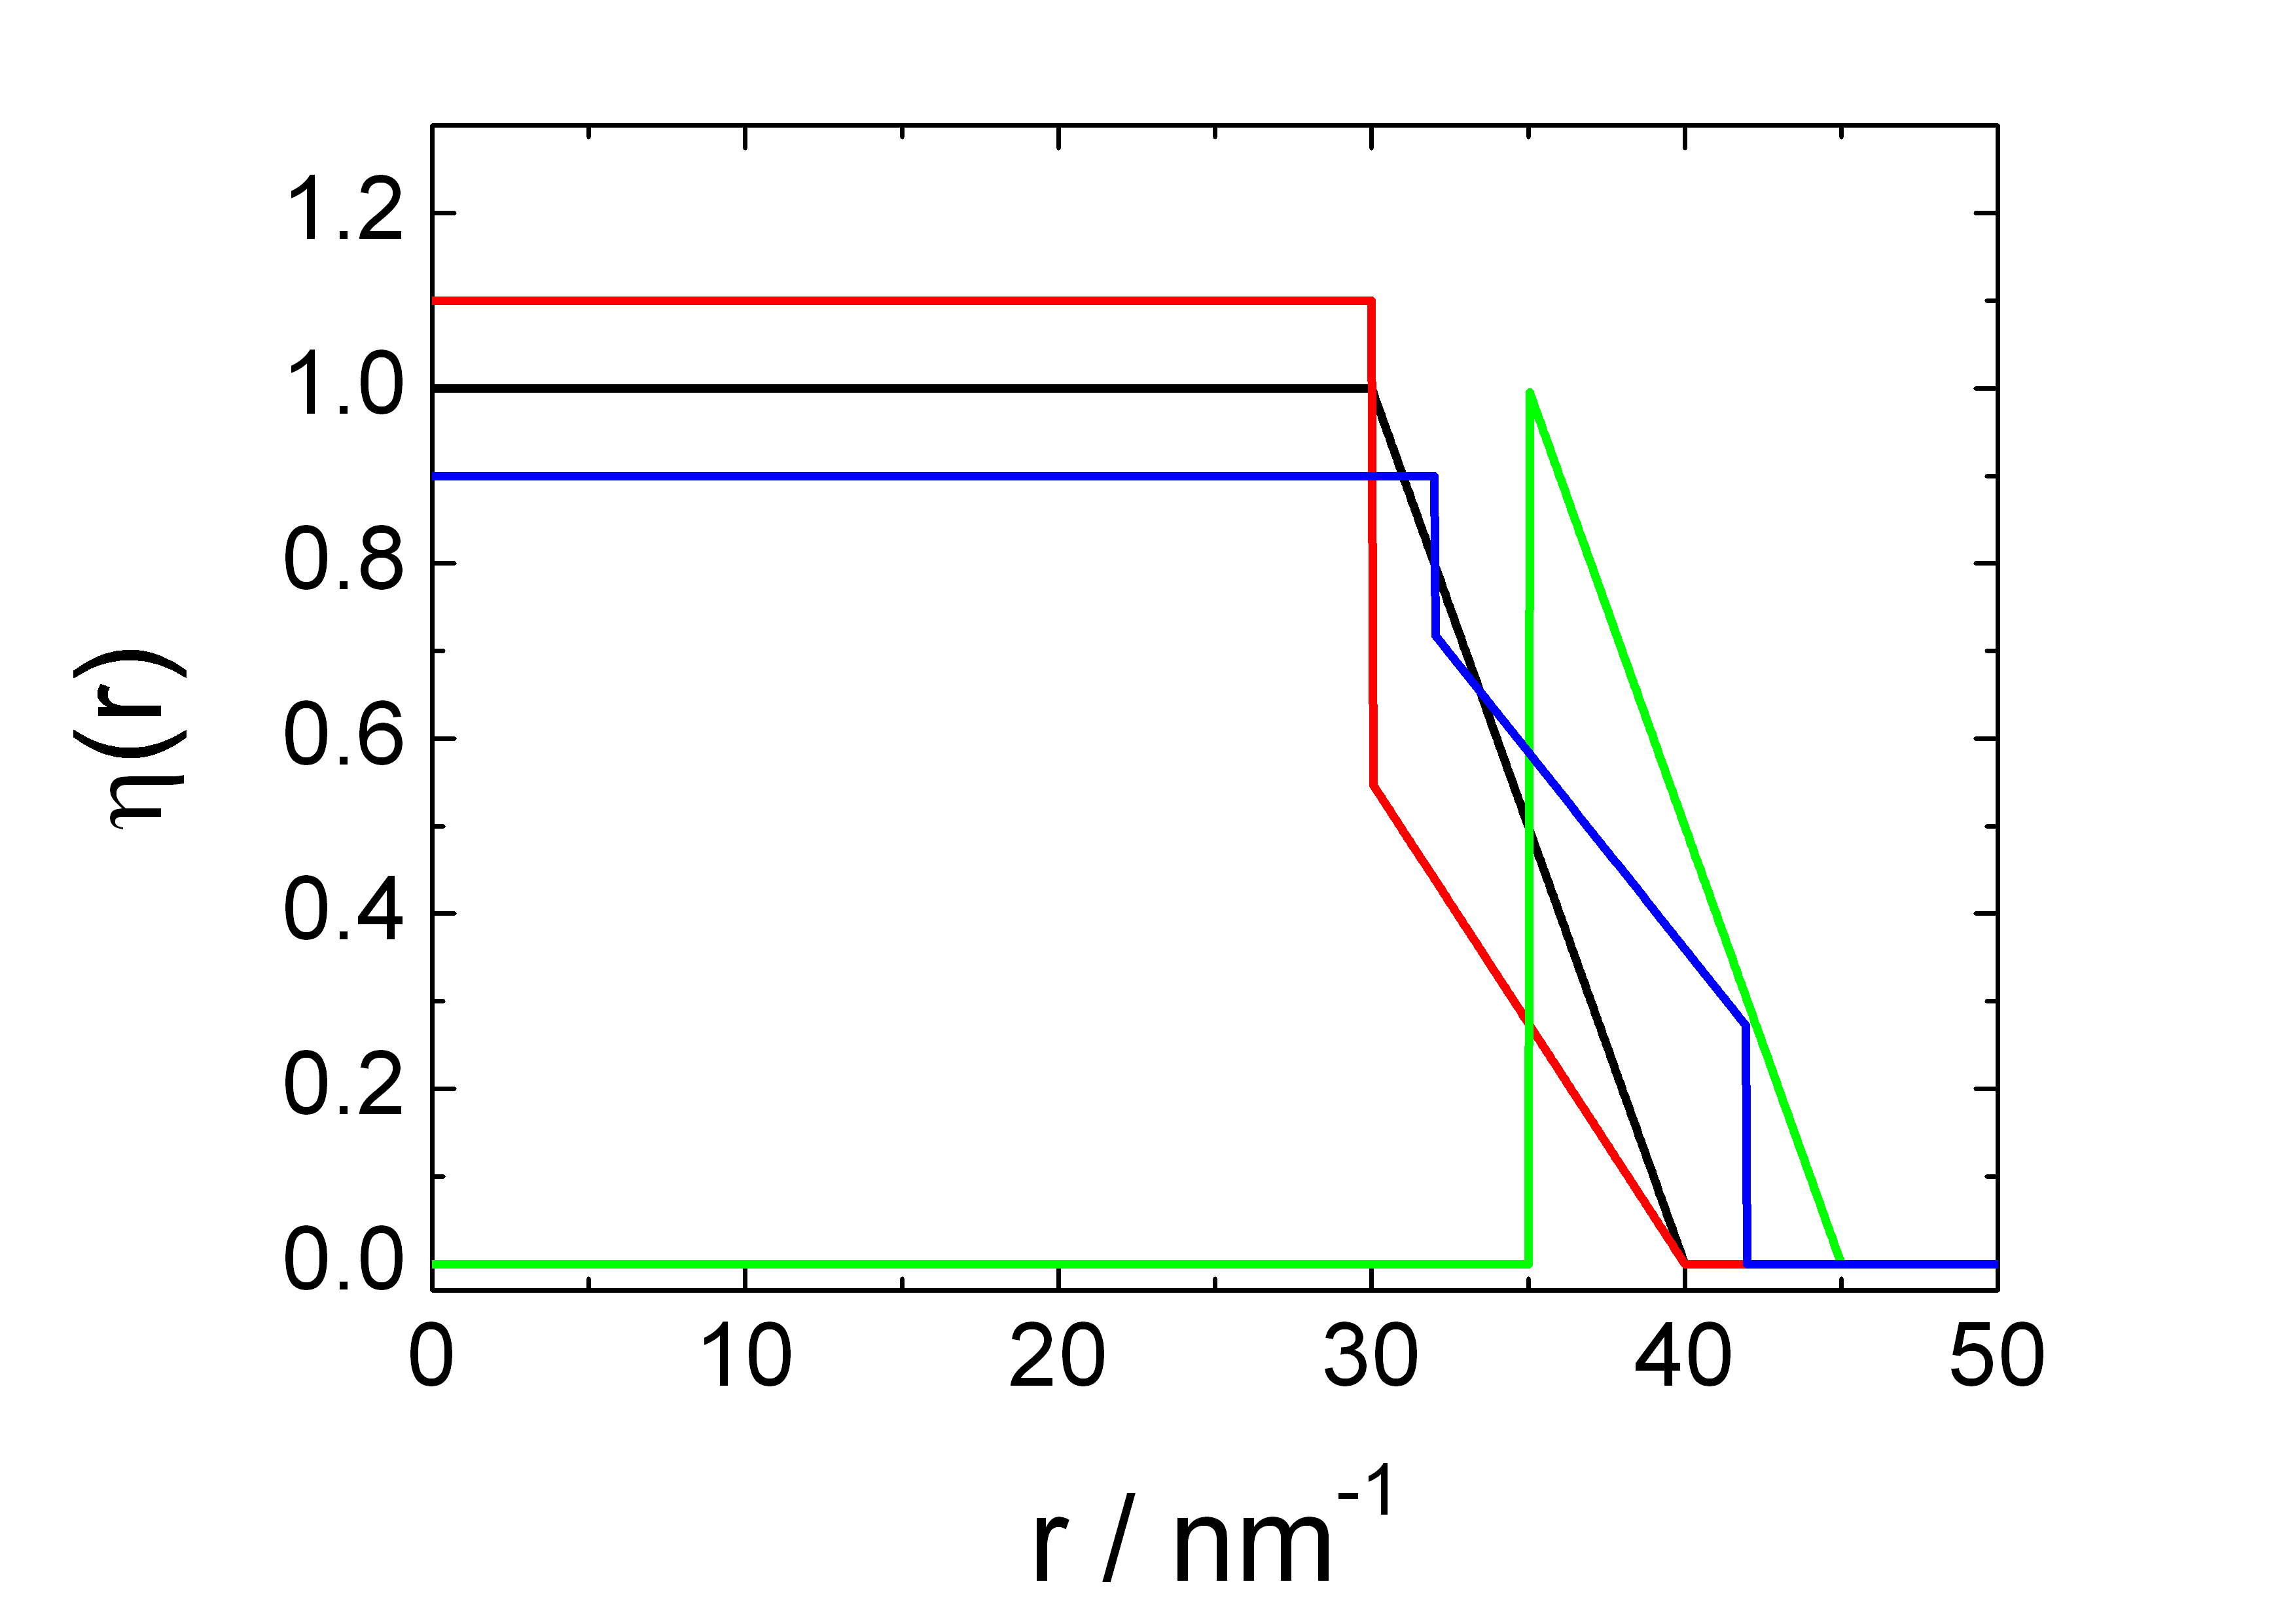
\includegraphics[width=0.48\textwidth,height=0.35\textwidth]{../images/form_factor/FuzzySphere/LinShell_profile.png}}
\hfill
\subfigure[Scattering curves of the radial profiles shown in Fig.\ (a).]{
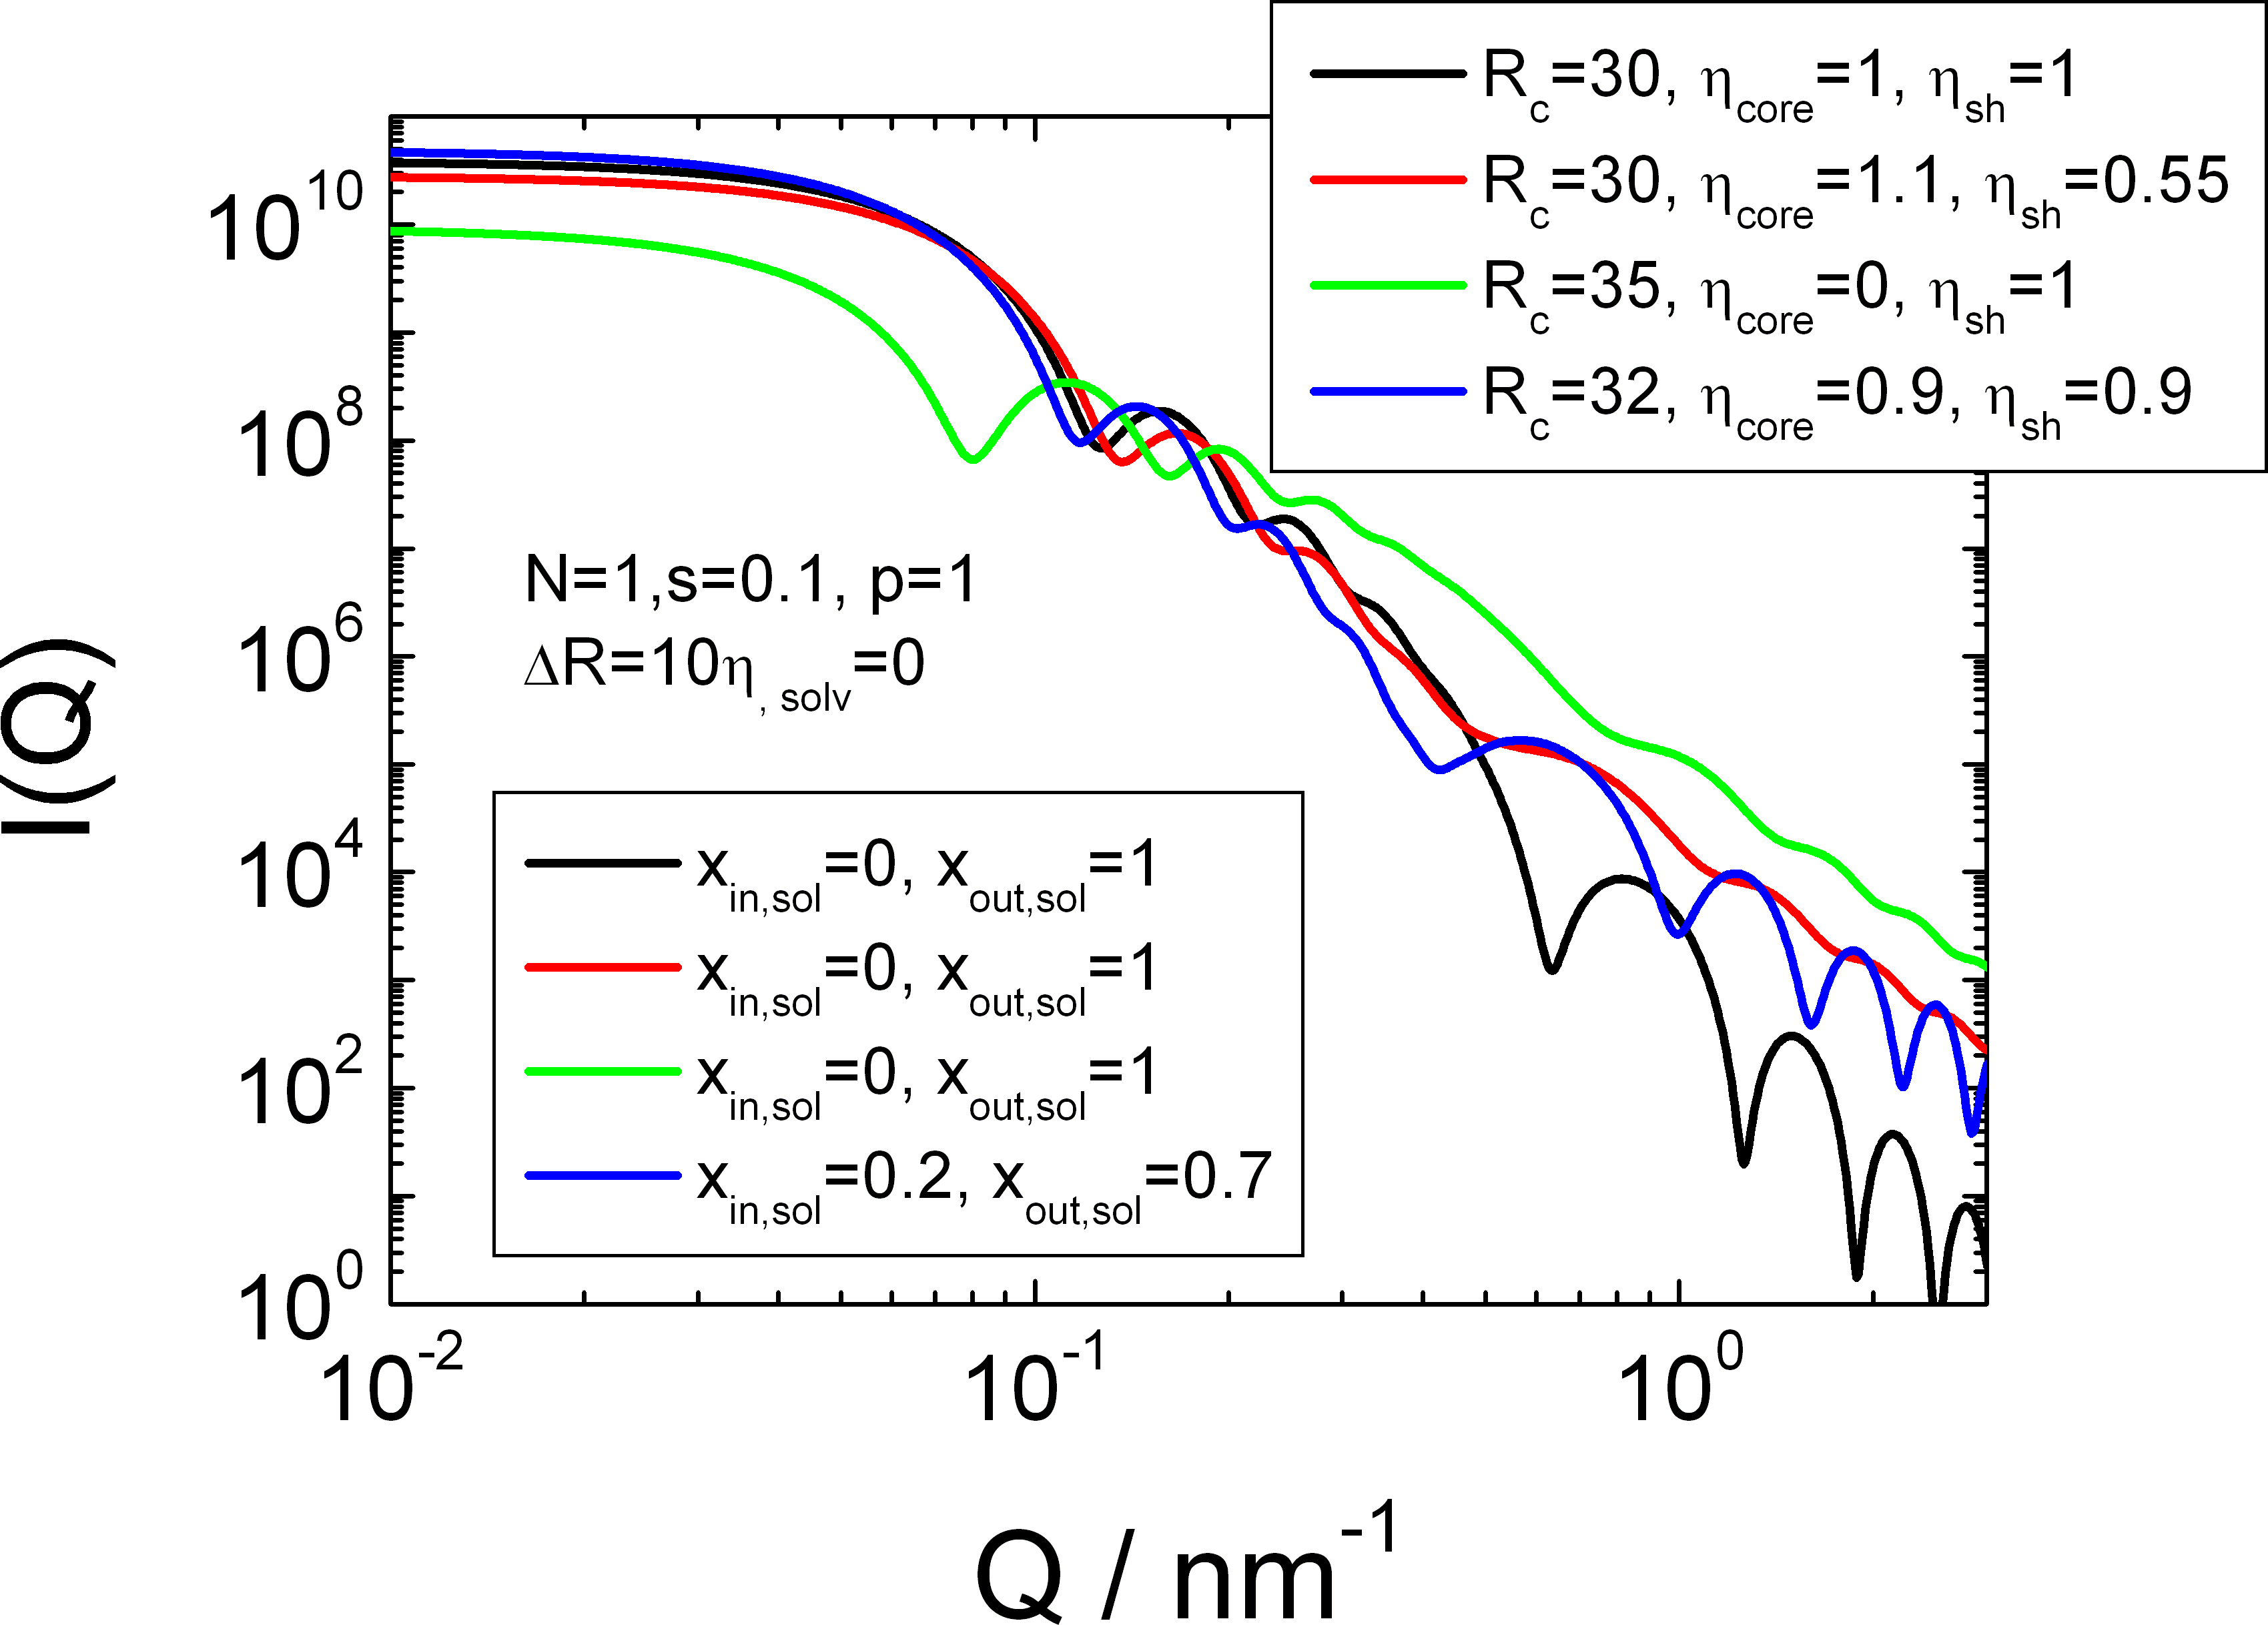
\includegraphics[width=0.48\textwidth,height=0.35\textwidth]{../images/form_factor/FuzzySphere/LinShell_IQ.png}}
\end{center}
\caption{Scattering intensity of a spherical shell with an linear shell profile. The scattering intensity has been calculated
with a lognormal size distribution for the core radius $R_c$.}
\label{fig:I_LinShell1}
\end{figure}
%%%%%%%%%%%%%%%%%%%%%%%%%%%%%%%%%%%%%%%%%%%%%%%%%%%%%%%%%%%%%%%%%%%%%%%%%

\clearpage
\subsubsection{LinShell2}
\label{sect:LinShell2} ~\\

\begin{figure}[htb]
\begin{center}
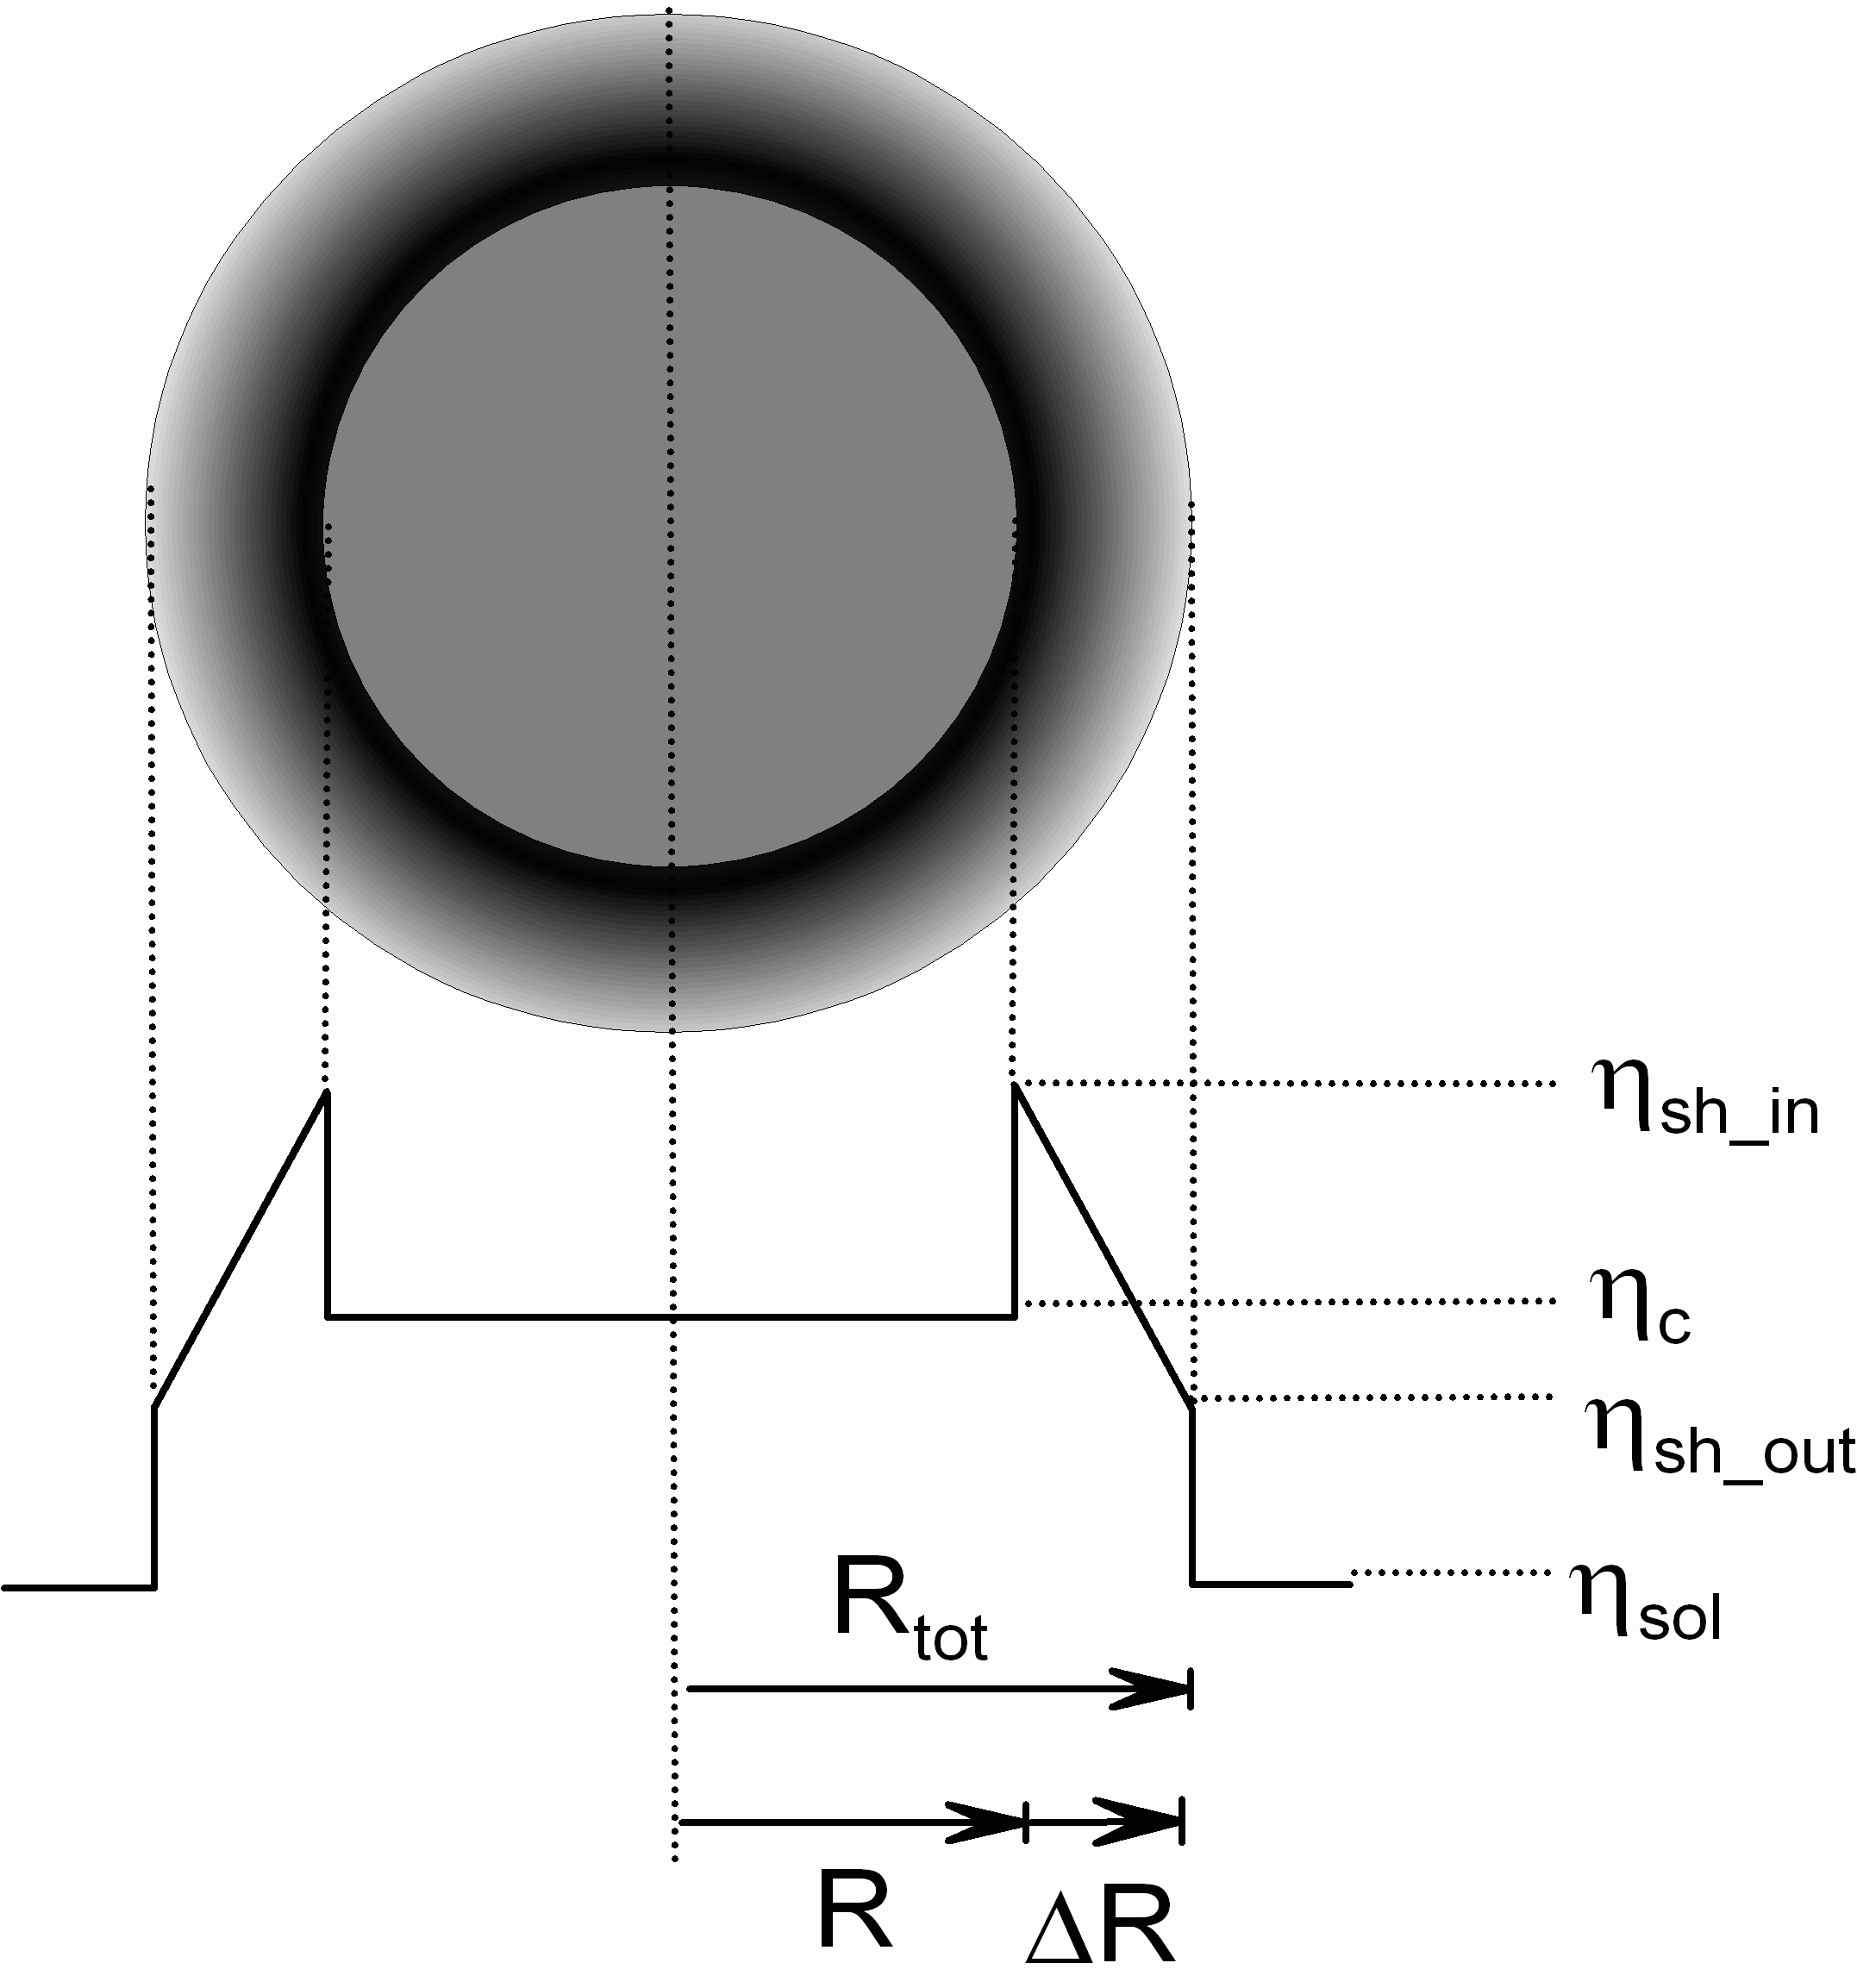
\includegraphics[width=0.5\textwidth,height=0.533\textwidth]{../images/form_factor/spheres/linshell2.png}
\end{center}
\caption{Radial profile for calculating the form factor of a spherical shell with a total
radius $R_\text{tot}$, a shell thickness of $\Delta R$, and a linear varying contrast
profile.} \label{LinShell2Profile}
\end{figure}

Form factor of a spherical shell with a total radius
$R_\text{tot}$ and a shell thickness of $\Delta R$. The definition
are the same than for {\tt LinShell} except that instead of the
core radius $R$ now the total radius $R_\text{tot}$ is used to
parameterize the form factor. The parameter definitions are the
following:
\begin{align}
R&=
\begin{cases}
R_\text{tot}-\Delta R & \mbox{for } R_\text{tot} > \Delta R \\
0 & \mbox{otherwise}
\end{cases}
\end{align}
\begin{align}
\Delta\eta(r)      & =
\begin{cases}
\eta_\text{c} & \text{~for~} r<R \\
m r + b  & \text{~for~} r \in [R,R_\text{tot}] \\
\eta_\text{sol} & \text{~for~} r>R_\text{tot}
\end{cases}
\end{align}
with
\begin{align}
m           & = (\eta_\text{sh\_out}-\eta_\text{sh\_in}) / \Delta R \\
b           & = -m R + \eta_\text{sh\_in}
\end{align}
and
\begin{align}
\eta_\text{sh\_in}  & = (1 - x_\text{in,sol})  \, \eta_\text{sh} + x_\text{in,sol} \,\eta_\text{sol} \\
                    & : \text{scattering length density at $R$} \nonumber \\
\eta_\text{sh\_out} & = (1 - x_\text{out,sol}) \, \eta_\text{sh} + x_\text{out,sol}\,\eta_\text{sol} \\
                    & : \text{scattering length density at $R_\text{tot}=R+\Delta R$} \nonumber \\
\eta_\text{sh}      & : \text{scattering length density of pure shell material} \nonumber \\
\eta_\text{c}       & : \text{scattering length density of core} \nonumber \\
x_\text{in,sol}     & : \text{amount of solvent at $R$} \nonumber \\
x_\text{out,sol}    & : \text{amount of solvent at $R_\text{tot}=R+\Delta R$} \nonumber
\end{align}

\begin{align}
F_\text{sph}(A,x) & = \frac{4}{3}\pi x^3 \,\, 3\frac{\sin(A)-A\cos(A)}{A^3} \\[5mm]
F_\text{shlin}(A,x) & = 4\pi x^4 \frac{2\cos(A)+2A\sin(A)-A^2\cos(A)}{A^4} \\[5mm]
I_\text{LinShell2}    & = \big[ \,\, (\eta_\text{c}-\eta_\text{sol}-b)F_\text{sph}(QR,R) \nonumber \\
             & \hspace{6mm} - mF_\text{shlin}(QR,R) \\
             & \hspace{6mm} + mF_\text{shlin}\left(QR_\text{tot},R_\text{tot}\right) \nonumber \\
             & \hspace{6mm} + bF_\text{sph}\left(QR_\text{tot},R_\text{tot}\right) \big]^2 \nonumber
\end{align}

\vspace{5mm}

\hspace{1pt}\\
\underline{Input Parameters for model \texttt{LinShell2} and \texttt{radial profile of LinShell2}:}\\
\begin{description}
\item[\texttt{Rtot}] total overall radius $R_\text{tot}$
\item[\texttt{dR}] thickness of the shell $\Delta R$
\item[\texttt{eta\_c}] scattering length density $\eta_\text{c}$
\item[\texttt{eta\_sh}] scattering length density of non-swollen shell $\eta_\text{sh}$
\item[\texttt{x\_in}] amount of solvent $x_\text{in,sol}$ on core-shell interface at $R$ $(x_\text{in,sol} \in [0;1])$
\item[\texttt{x\_out}] amount of solvent $x_\text{out,sol}$ on shell-solvent interface at $R+\Delta R$ $(x_\text{out,sol} \in [0;1])$.
\item[\texttt{eta\_s}] scattering length density of solvent $\eta_\text{sol}$
\end{description}


\noindent\underline{Note:}
\begin{itemize}
\item $x_\text{in,sol}$ and $x_\text{out,sol}$ are only physical for values between 0 and 1.
\end{itemize}

%%%%%%%%%%%%%%%%%%%%%%%%%%%%%%%%%%%%%%%%%%%%%%%%%%%%%%%%%%%%%%%%%%%%%%%%%

\clearpage
\subsubsection{ExpShell}
\label{sect:ExpShell} ~\\

\begin{figure}[htb]
\begin{center}
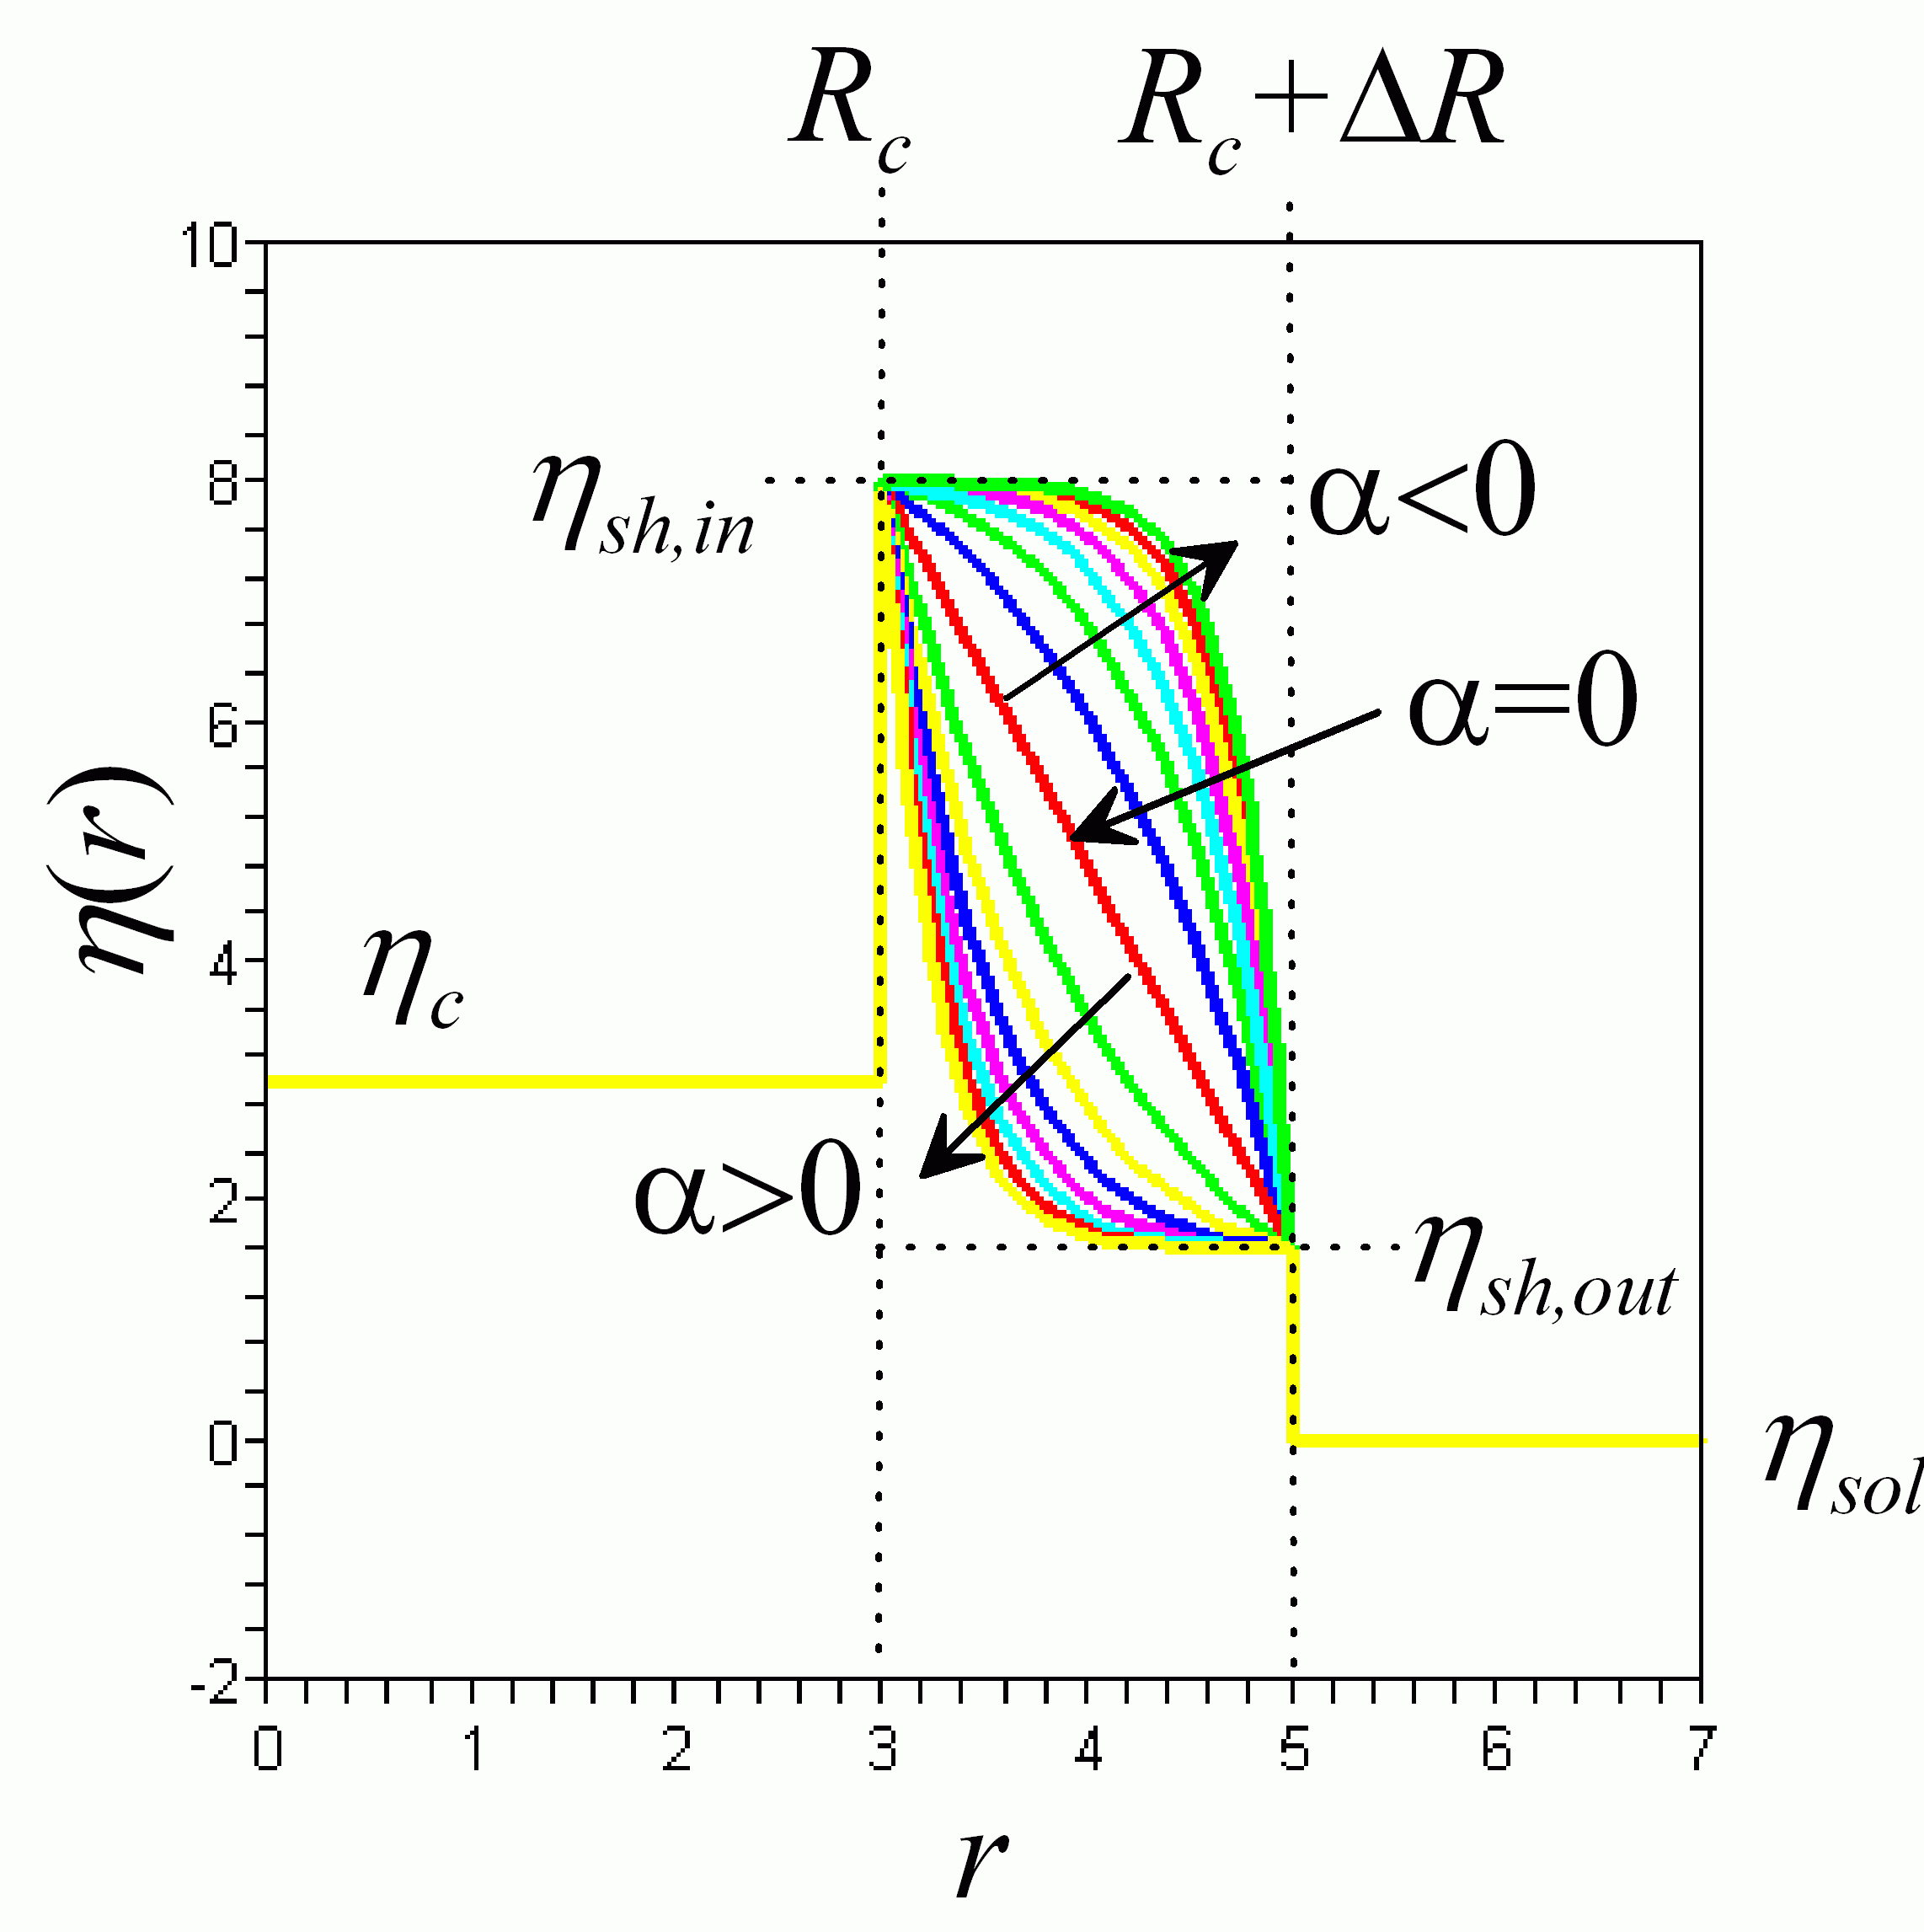
\includegraphics[width=0.55\textwidth,height=0.5\textwidth]{../images/form_factor/spheres/ExpShell.png}
\end{center}
\caption{Radial profile for calculating the form factor of a spherical shell with a core radius
$R_c$ and a shell thickness of $\Delta R$ and a exponentially varying contrast
profile. The profile shape can be varied by the parameter $\alpha$ describing the penetration of the solvent into the shell.
A value of $\alpha=0$ means linear profile and is equivalent to {\tt LinShell}
and {\tt LinShell2}. For $\alpha>0$ the solvent penetrates further into the shell
and for $\alpha<0$ less.} \label{ExpShellProfile}
\end{figure}

\noindent
\begin{align}
\eta_\text{ExpShell}(r,R_c,\Delta R,\alpha,\phi_\text{in},\phi_\text{out}) &=
\begin{cases}
\eta_c              & r \leq R_c  \\
\eta_\text{exp}(\frac {r-R_c}{\Delta R})   & R_c < r< R_c+\Delta R \\
\eta_\text{sol}     & r> R_c+\Delta R
\end{cases}
\end{align}
\begin{align}
\eta_\text{exp} (x) &=
\begin{cases}
\eta_\text{sh,in}  +
\left[\eta_\text{sh,out}-\eta_\text{sh,in}\right] x \exp\left( \left[ 1-x \right] \alpha\right)
 & \alpha<0 \\[2mm]
\left[\eta_\text{sh,in}-\eta_\text{sh,out}\right] \left[1-x\right] \exp\left(-{x\alpha}\right) +
 \eta_\text{sh,out}& \alpha \geq 0
\end{cases} \\[2mm]
\eta_\text{sh,in} & = \left[ \phi_\text{in}\,\eta_\text{sol}+ \left( 1-\phi_\text{in} \right)
 \eta_\text{sh} \right] \\
\eta_\text{sh,out} & = \left[ \phi_\text{out}\,\eta_\text{sol}+ \left( 1-\phi_\text{out} \right) \eta_\text{sh} \right]
\end{align}

The scattering intensity for the radial symmetric scattering length density profile $\eta_\text{ExpShell}(r)$
can be calculated analytical. The integral needed to be solved for that is
\begin{equation}
I_\text{ExpShell}(Q) = \int_0^\infty 4\pi r^2 \frac{\sin Qr}{Qr}\, \eta_\text{ExpShell}(r)\, dr
\end{equation}

\begin{align}
R_c &=\text{core radius} \nonumber\\
\Delta R &=\text{shell thickness} \nonumber\\
\eta_\text{sh,in}  & = (1 - \phi_\text{in,sol})  \, \eta_\text{sh} + \phi_\text{in,sol} \,\eta_\text{sol} \\
                    & : \text{scattering length density at $R_c$} \nonumber \\
\eta_\text{sh,out}     & = (1 - \phi_\text{out,sol}) \, \eta_\text{sh} + \phi_\text{out,sol}\,\eta_\text{sol} \\
                        & : \text{scattering length density at $R_c+\Delta R$} \nonumber \\
\eta_\text{sh}      & : \text{scattering length density of pure shell material} \nonumber \\
\eta_\text{c}       & : \text{scattering length density of core} \nonumber \\
\phi_\text{in}     & : \text{amount of solvent  at $R_c$} \nonumber \\
\phi_\text{out}    & : \text{amount of solvent at $R_c+\Delta R$} \nonumber \\
\alpha             & : \text{parameter for exponential diffuse profile of the shell} \\
\nonumber
\end{align}


\vspace{5mm}

\hspace{1pt}\\
\underline{Input Parameters for model \texttt{ExpShell}:}\\
\begin{description}
\item[\texttt{R\_core}] radius of core  $R_c$
\item[\texttt{DR}] thickness of the shell $\Delta R$
\item[\texttt{eta\_core}] scattering length density $\eta_\text{c}$
\item[\texttt{eta\_shell}] scattering length density of non-swollen shell $\eta_\text{sh}$
\item[\texttt{x\_in\_sol}] amount of solvent $\phi_\text{in}$ on core-shell interface at $r=R$
\item[\texttt{x\_out\_sol}] amount of solvent $\phi_\text{out}$ on shell-solvent interface at $r=R+\Delta R$
\item[\texttt{alpha}]  a parameter ($\alpha$) which describes the penetration profile of the solvent into the shell.
A value of $\alpha=0$ means linear profile and is equivalent to {\tt LinShell} and {\tt LinShell2}. For $\alpha>0$
the solvent penetrates further into the shell and for $\alpha<0$ less.
\item[\texttt{eta\_solvent}] scattering length density of solvent $\eta_\text{sol}$
\end{description}

\noindent\underline{Note:}
\begin{itemize}
\item $\phi_\text{in}$ and $\phi_\text{out}$ are only physical for values between 0 and 1.
\end{itemize}

\begin{figure}[htb]
\begin{center}
\subfigure[Some radial profiles of spheres with a exponential interfaces
which have been used to calculate the scattering curve in Fig.\ (b).
]{
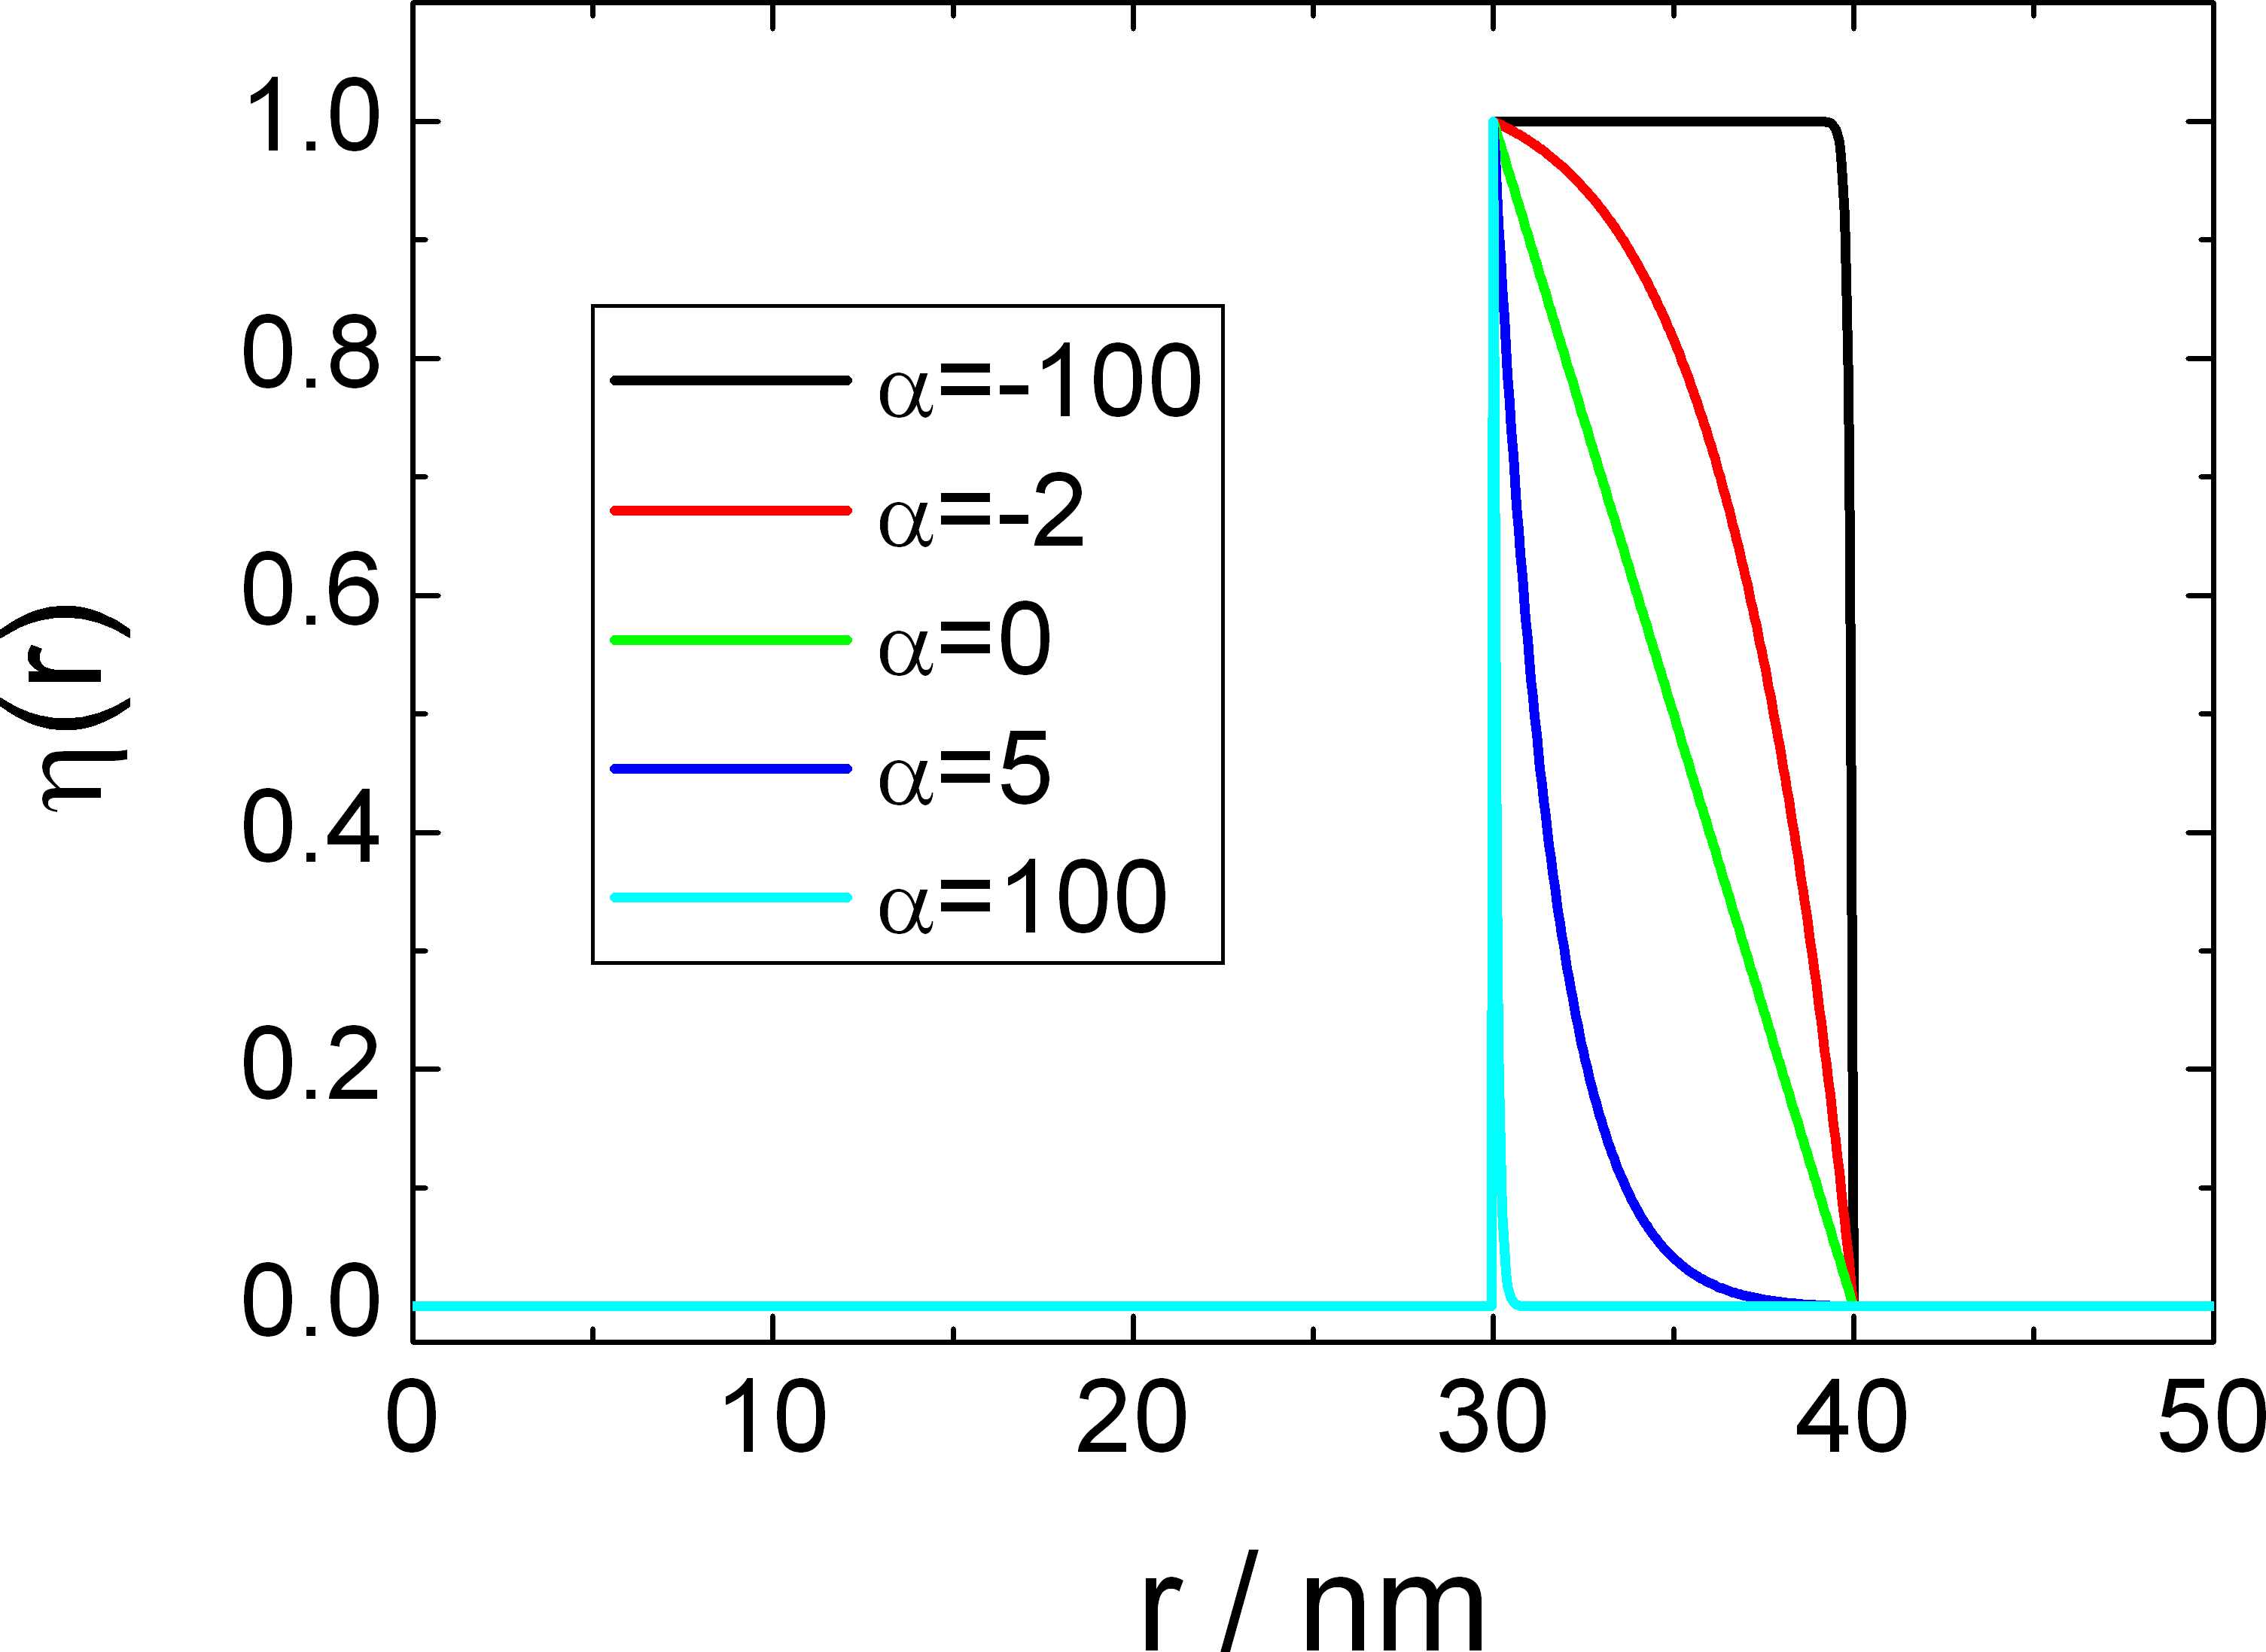
\includegraphics[width=0.48\textwidth,height=0.35\textwidth]{../images/form_factor/FuzzySphere/ExpShell_profile.png}}
\hfill
\subfigure[Scattering curves of the radial profiles shown in Fig.\ (a).]{
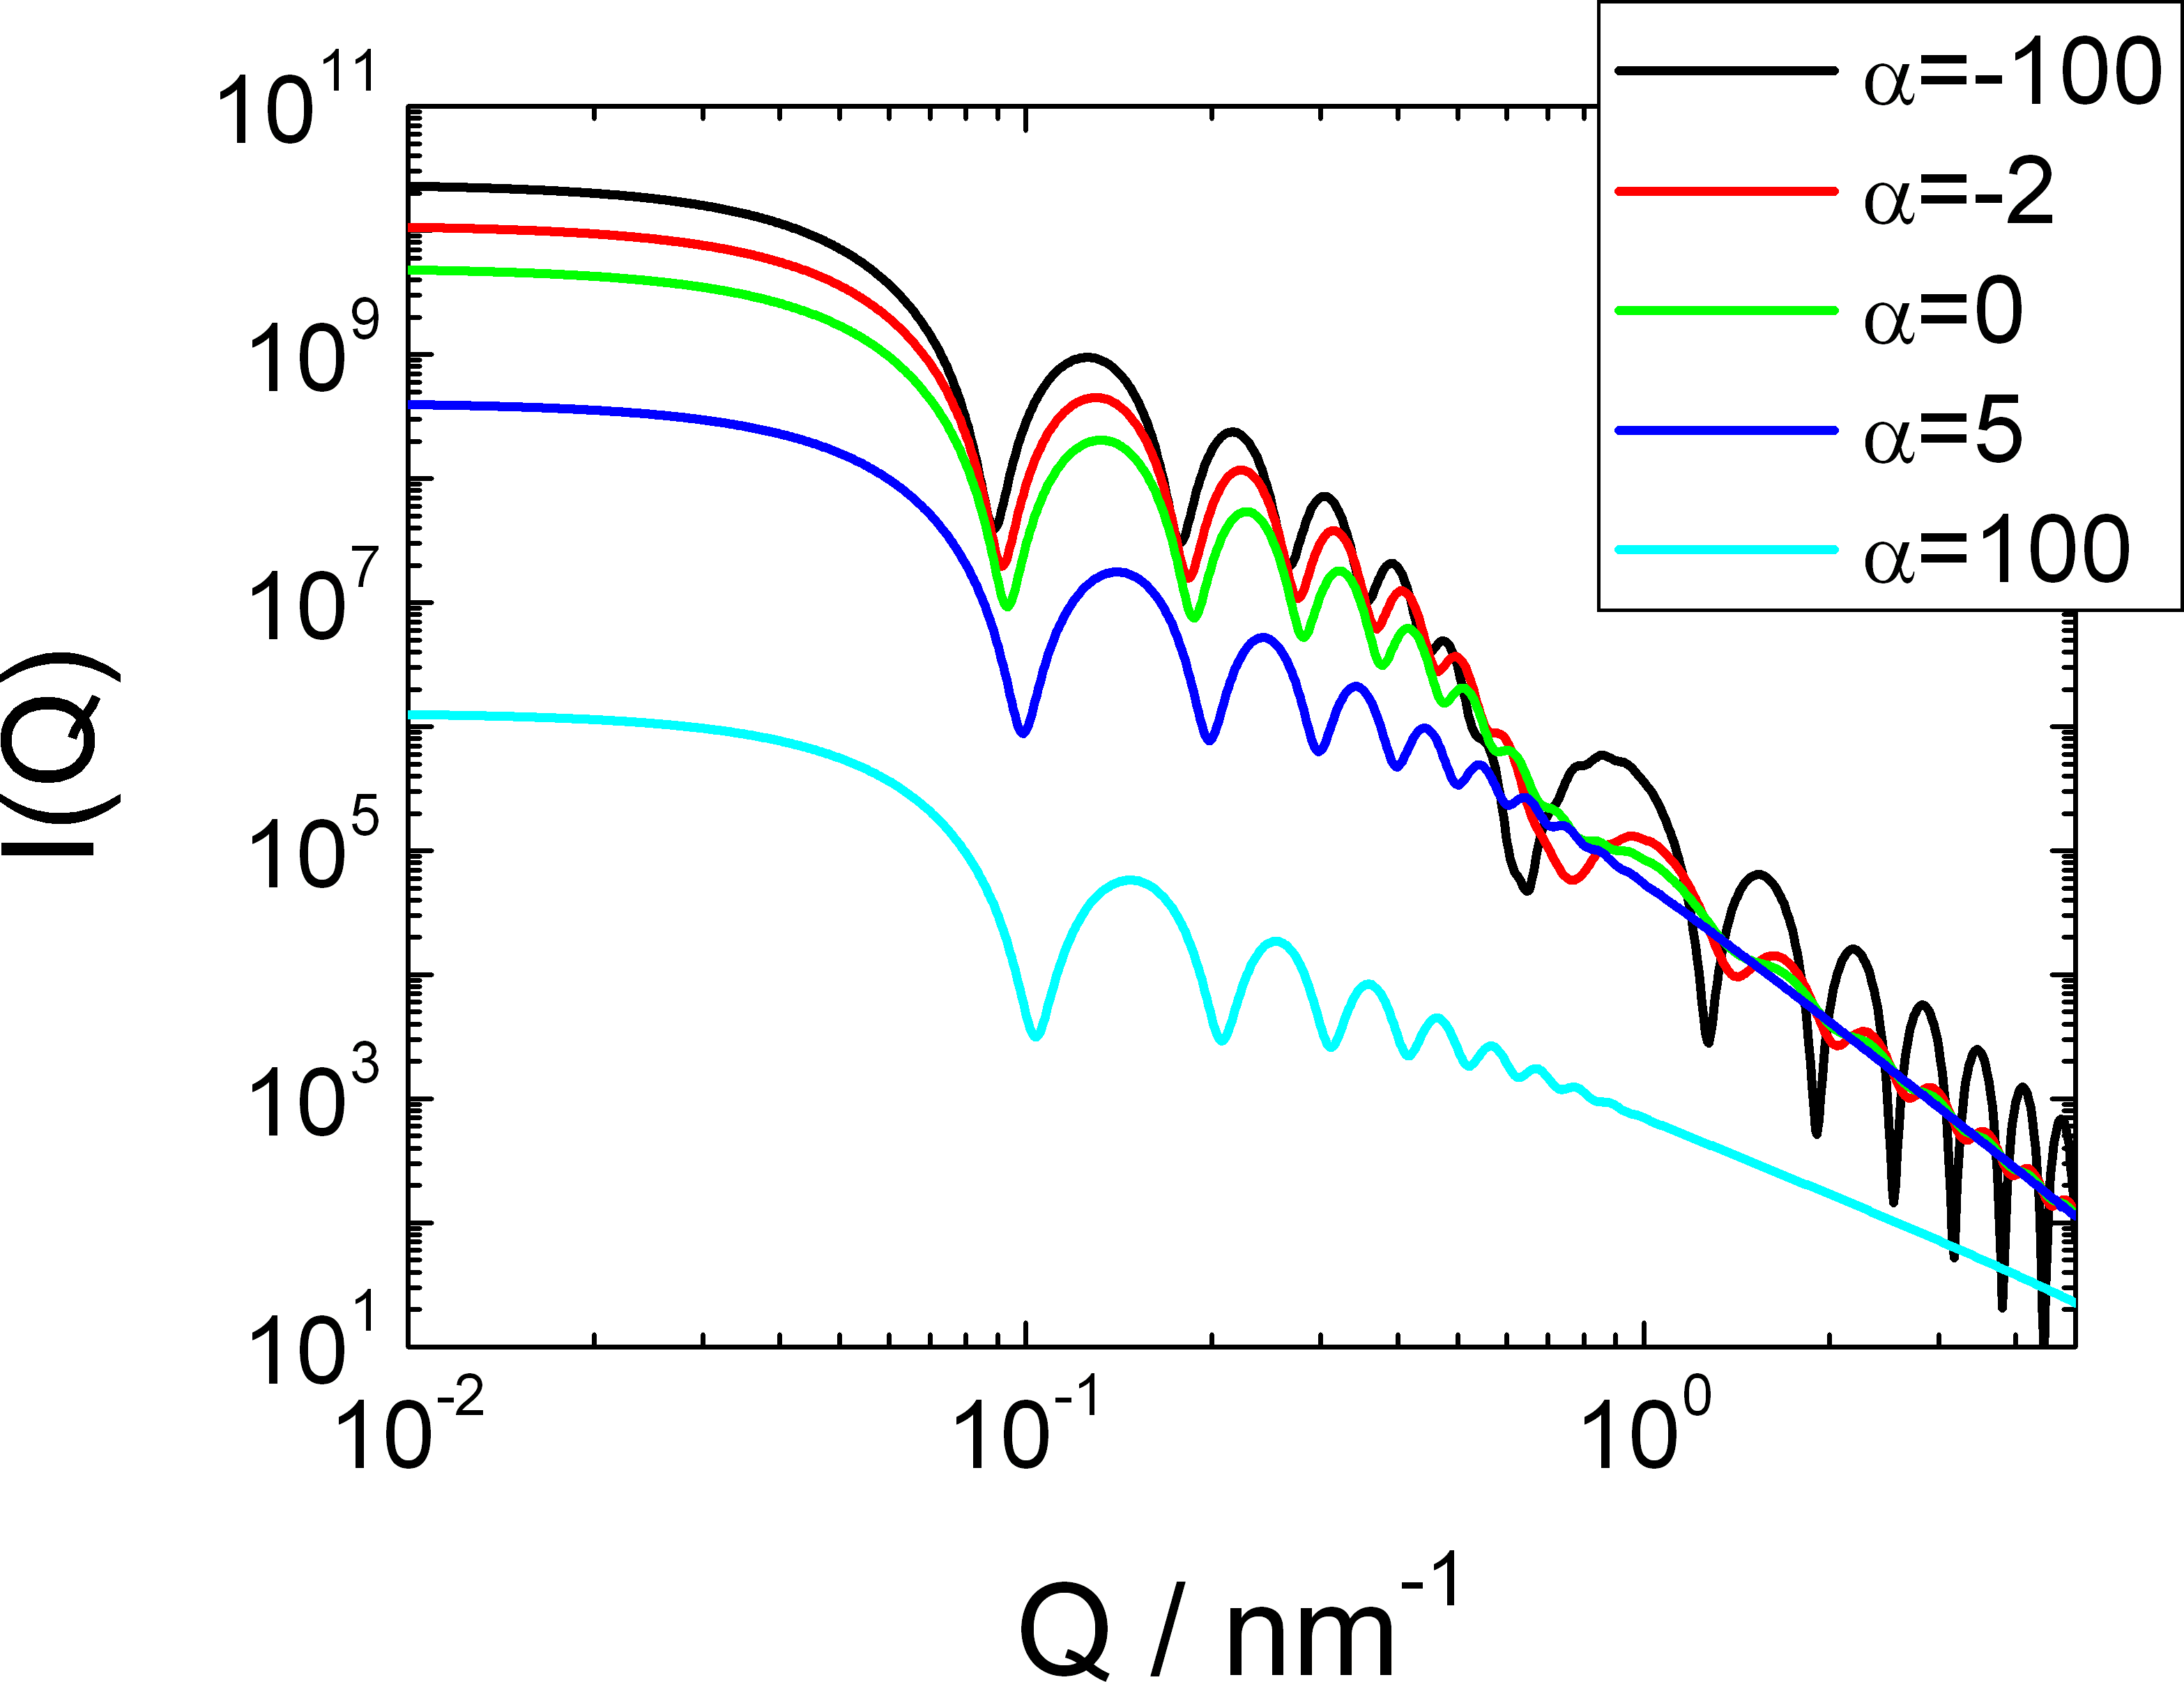
\includegraphics[width=0.48\textwidth,height=0.35\textwidth]{../images/form_factor/FuzzySphere/ExpShell_IQ.png}}
\end{center}
\caption{Scattering intensity of a spherical shell with an exponential shell profile. The scattering intensity has been calculated
with a lognormal $[\mathrm{LogNorm}(N\!=\!1,\sigma\!=\!0.05,p\!=\!1,R\!=\!30)]$ size distribution for the core radius $R_c$.
The scattering length density of the core $\eta_\text{c}$ and the solvent $\eta_\text{sol}$ are set to 0, $\eta_\text{sh}=1$,
$\phi_\text{in}=0$,  $\phi_\text{out}=1$, and $\Delta R =10$.}
\label{fig:ExpShellExample}
\end{figure}

%%%%%%%%%%%%%%%%%%%%%%%%%%%%%%%%%%%%%%%%%%%%%%%%%%%%%%%%%%%%%%%%%%%%%%%%%%%%%%%%%%%%%%%%
\clearpage
\section{Magnetic spin misalignment} \hspace{1pt}
\label{sec:spinmisalignment}

In \cite{Michels2013} the autocorrelation function $C(r)$ of the
spin misalignment has been published. The approach assumes the
material to be close to magnetic saturation and considers uniform
values for the exchange interaction and the saturation
magnetization, i.e. it's a micro magnetic theory of single phase
magnets. The correlation function is defined by
\begin{align}
C(r) & = \frac{K R^4}{H_i^2} \int_0^\infty
\frac{j_0(qr)j_1^2(qR)}{\left(1+l_H^2q^2\right)^2} d\text{q}
\end{align}
where $j_1$ and $j_2$ are the spherical Bessel
functions\footnote{the spherical Bessel functions $j_n$ and $y_n$,
and are related to the ordinary Bessel functions $J_n$ and $Y_n$ by:
 $j_{n}(x) = \sqrt{\frac{\pi}{2x}} J_{n+\frac{1}{2}}(x)$ and $
 y_{n}(x) = \sqrt{\frac{\pi}{2x}} Y_{n+\frac{1}{2}}(x) = (-1)^{n+1}
 \sqrt{\frac{\pi}{2x}}J_{-n-\frac{1}{2}}(x)$.
 The first two spherical Bessel function are computed by
 $j_0(x)=\frac{\sin(x)} {x}$ and
 $j_1(x)=\frac{\sin(x)} {x^2}- \frac{\cos(x)} {x}$} and $K=8H_P^2/V$.
 $H_i$ is the internal magnetic field, $l_H=\sqrt{2A/(\mu_0 M_s H_i)}$
 the exchange length of the magnetic field, $H_P$ the mean magnetic
 anisotropy field, $A$ the exchange-stiffness constant, and $\mu_0$
 the permeability of free space. The internal magnetic field
 $H_i=H_0-NM_s$ is the sum of the external applied magnetic field
 $H_0$ and the demagnetisation field $-NM_s$ ($N$: demagnetisation
 factor). $V$ is the sample volume and $M_s$ the saturation
 magnetisation.

It is assumed in this model that the magnetic anisotropy field,
which perturbs the magnetization from the homogeneously magnetized
state, is uniform (constant) within a spherical volume; the
parameter $R$ represents the corresponding �anisotropy-field�
radius, and it is emphasized that $R$ is not necessarily identical
to the crystallite size.

The correlation is related to the scattering intensity by
\begin{align}
C(r) &= \frac{1}{2\pi^2} \int_0^\infty I(q) q^2
\frac{\sin(qr)}{qr}d\text{q}
 \frac{1}{2\pi^2} \int_0^\infty I(q) q^2 j_0(qr) d\text{q}
\end{align}
Therefore the intensity can be easily seen that $I(q)$ can be
computed as
\begin{align}
I(q) & = \frac{K R^6}{H_i^2}
\frac{2\pi^2}{\left(qR\right)^2}\frac{j_1^2(qR)}{\left(1+l_H^2q^2\right)^2}
\end{align}

\vspace{5mm}

\hspace{1pt}\\
\underline{Input Parameters for the models \texttt{C(r) for spin
misalignment} and} \newline \underline{\texttt{I(q) for spin misalignment}:}\\
\begin{description}
\item[\texttt{K}] $K=8H^2_P/V$
\item[\texttt{H\_i}] internal magnetic field $H_i$
\item[\texttt{l\_H}] exchange length of magnetic field $l_H$
\item[\texttt{R}] anisotropy field radius $R$
\end{description}

\noindent\underline{Note:}
none


\begin{figure}[htb]
\begin{center}
\subfigure[The scattering curves for the correlation functions on to
right]{
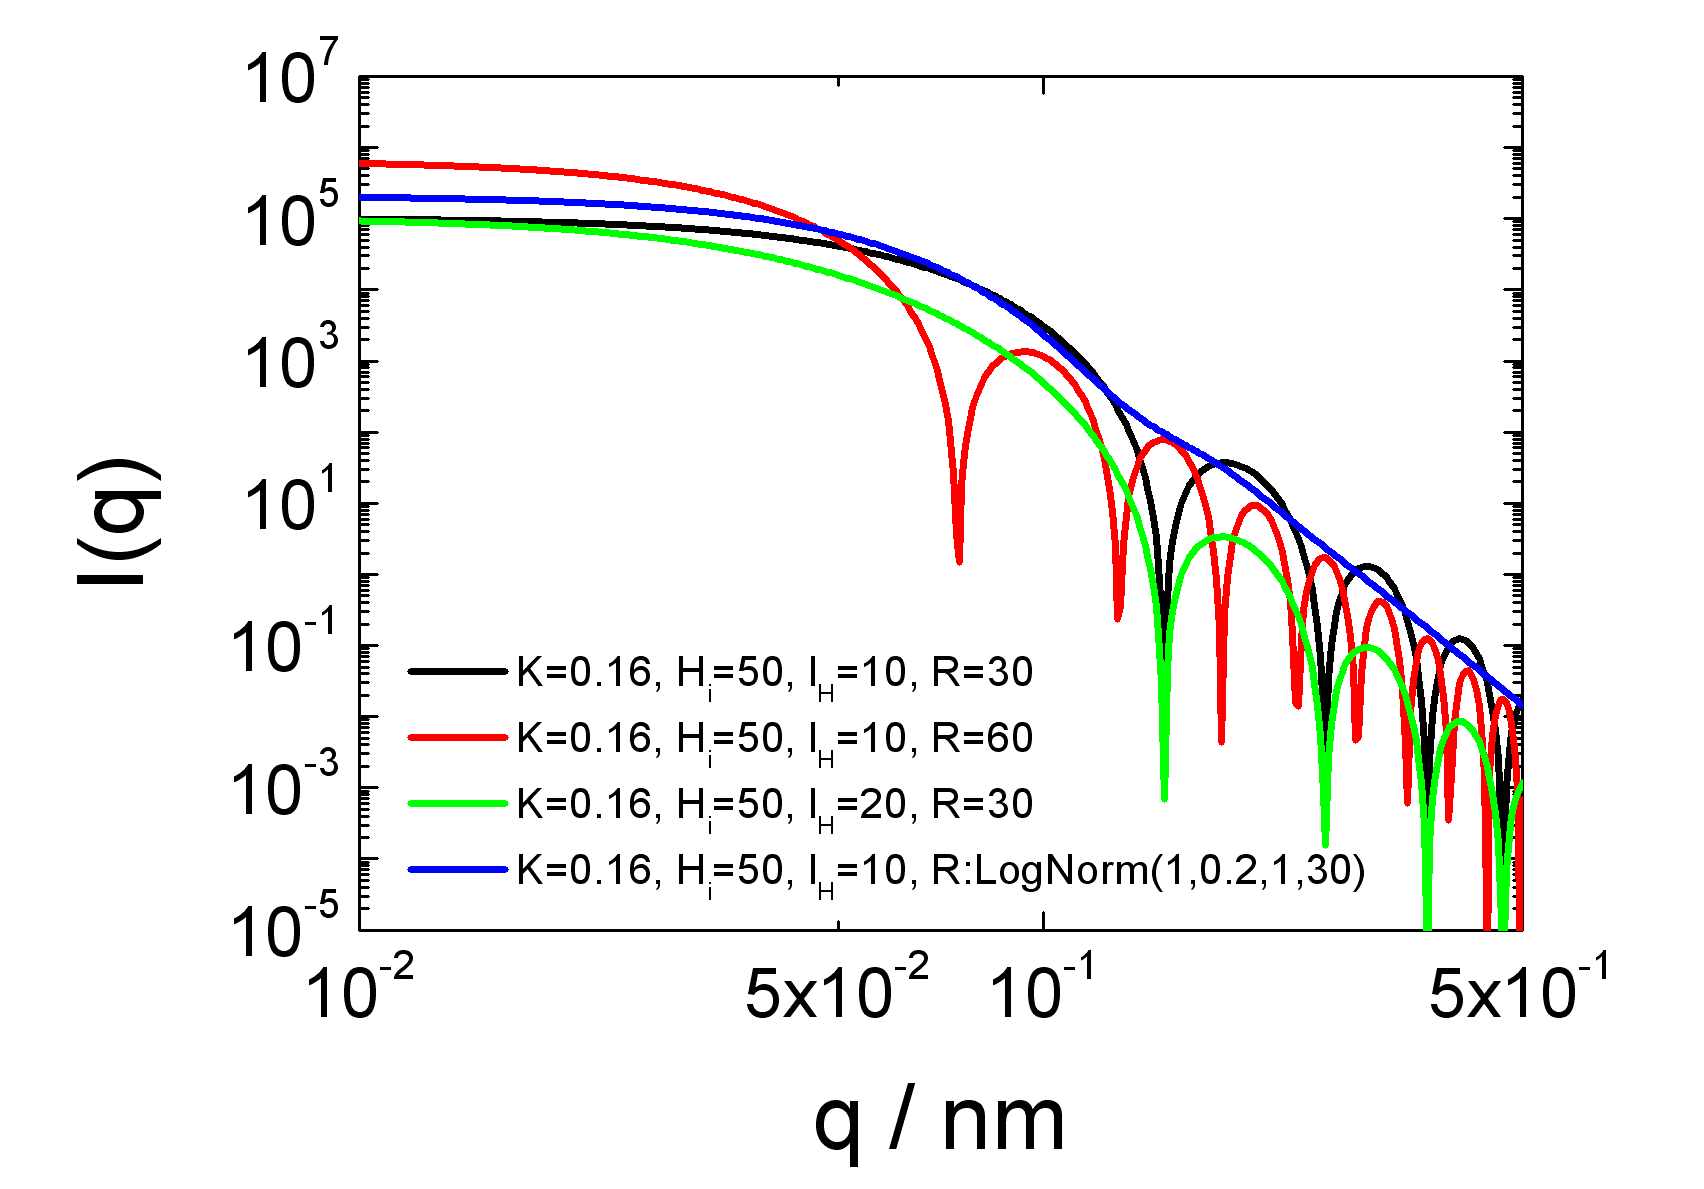
\includegraphics[width=0.48\textwidth,height=0.35\textwidth]{../images/form_factor/magnetic/IQ4spinmisalignment.png}}
\hfill \subfigure[correlation functions for the scattering curves to
the left]{
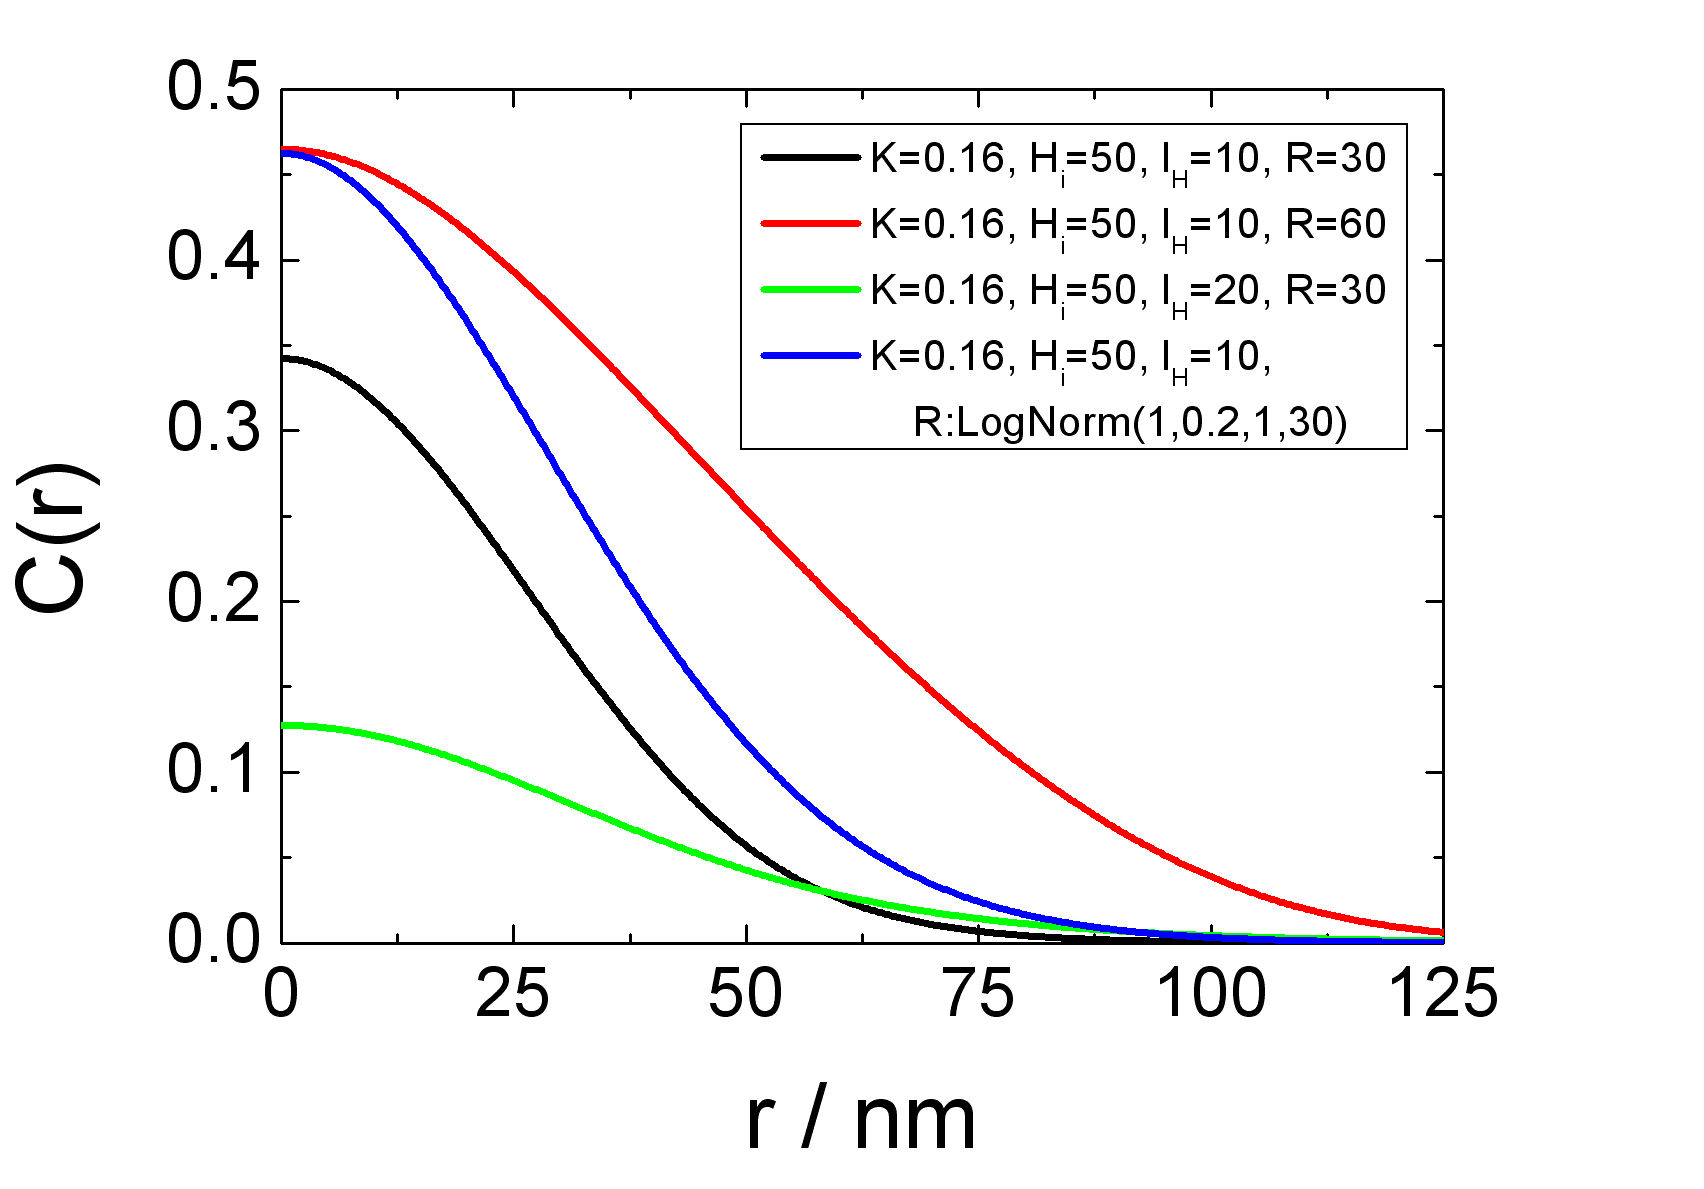
\includegraphics[width=0.48\textwidth,height=0.35\textwidth]{../images/form_factor/magnetic/correlation4spinmisalignment.png}}
\end{center}
\caption{Scattering curves and corresponding correlation functions.
In one case the radius of the anisotropy field is assumed to have a
lognormal size distribution.} \label{fig:MagSpinMisAlignment}
\end{figure}


%%%%%%%%%%%%%%%%%%%%%%%%%%%%%%%%%%%%%%%%%%%%%%%%%%%%%%%%%%%%%%%%%%%%%%%%%%%%%%%%%%%%%%%%
\clearpage
\section{Ferrofluids} \hspace{1pt}
\label{sec:ferrofluid}

"Ferrofluids" and "Magnetic Liquids" are two common expressions for
suspensions in which nanometer sized particles are dispersed in a
carrier liquid. Figure \ref{fig:ferrofluidparticle} gives a
schematic illustration. The particle material can be ferri- or
ferromagnetic, and is often coated with a stabilizing dispersing
agent (surfactant). The particle size is smaller than the size of
magnetic domains of the corresponding bulk material. This means that
every particle is single-domain ferri- or ferromagnetic.
Additionally we assume in this model, that the metallic core has a
shell structure to be able to model a thin oxidation layer with a
reduced magnetisation on the surface.The surfactant molecules
consist of a head and a polar tail. The head can coalesce with the
magnetic particle, and the tail protrudes into the carrier liquid
and can dissolve in it. This polar tails protruding into the liquid
lead to repulsion between the colloids. Different substances like
organic acids or polymers usually serve as surfactants. The carrier
liquid is selected to meet the requirements for a particular
applications: It can be hydrocarbon, ester, water or others. As a
result of the small size of the particles they are very mobile due
to Brownian motion. In zero field the magnetic moment is random
oriented. Applying a magnetic field the orientation distribution of
the magnetic moments of the ferrofluid particles follow a Langevin
statistic.

\begin{figure}[htb]
\begin{center}
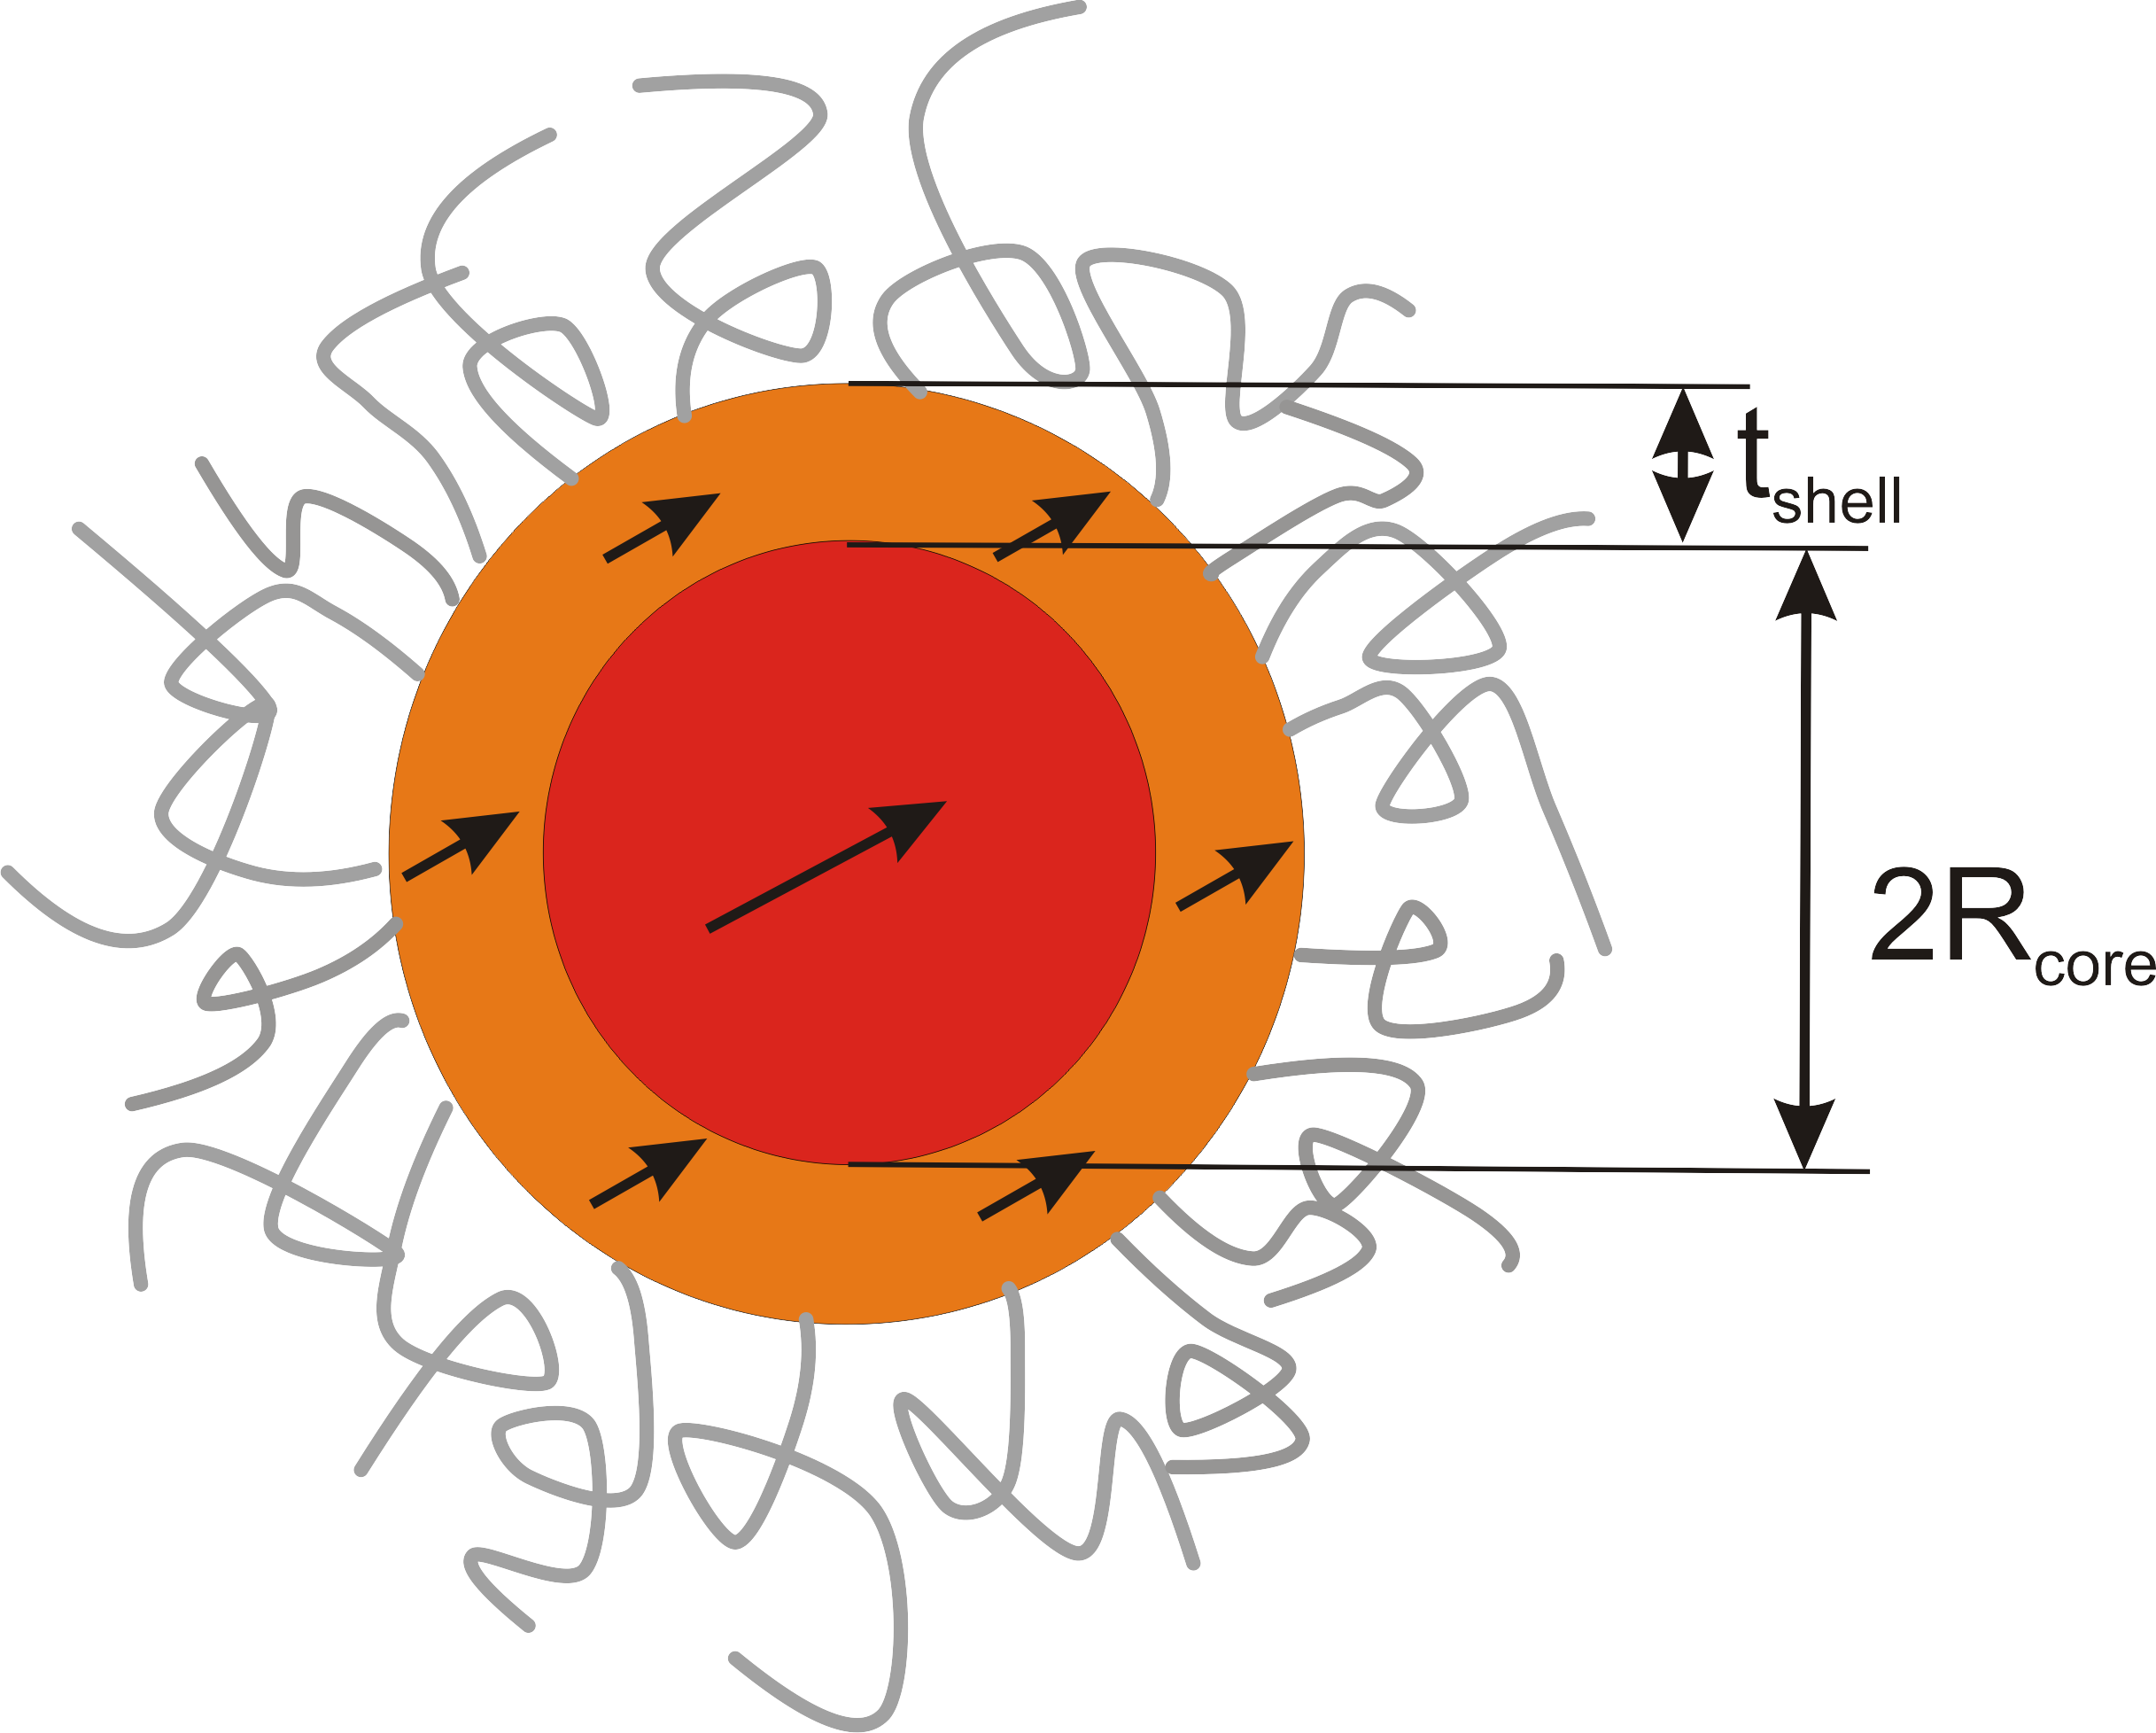
\includegraphics[width=0.6\textwidth]{../images/form_factor/ferrofluid/ferrfluidparticle.png}
\end{center}
\caption{Sketch of a ferrofluid particle stabilised with surfactant
molecules on its surface. The magnetic core can have a shell with
lower magnetisation. The direction of the shell magnetisation is
assumed to be parallel or antiparallel to the core magnetisation,
depending on the signs of the magnetic scattering length densities.}
\label{fig:ferrofluidparticle}
\end{figure}

In the present implementation of scattering function of
superparamagnetic particles geometrical parameters are calculated
like magnetic scattering length densities are calculated from the
magnetization of the shell and the core, whereas the nuclear
scattering length densities are an explicit input parameter. In such
a case one has to be careful using the right units.

The relevant parameters to describe the ferrofluid particle in this
model are:
\begin{itemize}
\item Radius of the $R_\text{core}$ in reciprocal units of scattering vector $q$.
\item Thickness of the metallic shell $t_\text{shell}$ in reciprocal units of scattering vector $q$.
\item Specific aggregation number of stabilizing surfactant molecules per surface area in units of cm$^{-2}$.
\item Molecular volume $V_\text{brush}$ of a single surfactant molecule in units of nm$^3$.
The scattering length density calculator of \SASfit might be useful
to supply this value.
\item Nuclear scattering length density $\eta_\text{core}$ of the solid ferromagnetic core.
\item Nuclear scattering length density $\eta_\text{sh}$ of an optional demagnetised shell of the
solid ferromagnetic core.
\item Nuclear scattering length density of the solvent $\eta_\text{solv}$.
\item Magnetisation of the metallic core $M_\text{core}$.
      The magnetic scattering length density is calculated via eq.\ \ref{eq:magnetic_SLD}.
\item Magnetisation of the metallic shell $M_\text{sh}$.
      Also here the magnetic scattering length density of the shell is calculated via eq.\ \ref{eq:magnetic_SLD}.
\item Temperature $T$ in Kelvin.
\item External applied magnetic field $B$ in Tesla or milliTesla depending of the units of $q$.
\item Lagrange parameter $\alpha$ for describing superparamagnetic properties is calculated by ratio
of the potential energy of the total magnetic moment of the superparamagnetic particle in the applied magnetic
field to the thermal energy via eq.\ \ref{eq:alpha}
\item As aligned magnetic structures scatter anisotropically the angle $\psi$ between scattering vector
and the applied magnetic field needs to be supplied.
\item using polarised neutrons the incident polarisation $p$ needs to be known. $p$ can have values $p \in [-1,1]$.
\item in case of full polarisation analysis also the transmission of the analyser needs to be known
\end{itemize}

The magnetic scattering length density $\eta_\text{mag}$ in units of
cm$^{-2}$ is calculated from the magnetisation $M$ given in units of
A/m by
\begin{align}
\eta_\text{mag} &= D_M \mu_0 M \label{eq:magnetic_SLD} \times 10^{-4}\\
D_M & = 2.3161 \frac{1}{\text{Vs}} \\
\mu_0 &= 4\pi \times 10^{-7} \text{H}\text{m}^{-1} = 4\pi \times 10^{-7} \frac{\text{Vs}}{\text{Am}}
\end{align}
To get the magnetic scattering length density in cm$^{-2}$ a
multiplication factor of $10^{-4}$ has to be applied. By choosing
the unit cm$^{-2}$ for the magnetic scattering length density we
have to use the corresponding units for the nuclear scattering
length densities.

The other unit which has to be chosen with care is the molecular
volume $V_\text{brush}$ of a single surfactant molecule. From the
specific aggregation and the molecular volume the excess scattering
of the surfactant shell is calculated. In case that the $q$-values
are given in units of nm$^{-1}$ the molecular volume has to be in
units of  nm$^3$ and in case of \AA$^{-1}$ for the q-values one also
need to use \AA$^{3}$ units for the molecular volume.

The next parameter, where we need to use proper units is the
Langevin parameter $\alpha$, describing the ratio between potential
energy of the magnetic moment of the particle to the thermal energy:
\begin{align}
\alpha &= \mu_\text{FF}B/(k_B T) \label{eq:alpha} \\
\mu_\text{FF} &= \frac{4}{3}\pi
\left[ R_\text{core}^3  M_\text{core} +
\left\{\left(R_\text{core}+t_\text{shell}\right)^3-R_\text{core}^3\right\} M_\text{shell}
\right] \times \frac{10^{-27}\text{m}^3}{\text{nm}^3}\label{eq:mu_FF}\\
k_\text{B} &= 1.3806488 \times 10^{-23} \text{m}^2 \text{kg} \text{
s}^{-2} \text{K}^{-1}
\end{align}
The magnetic moment of a particle $\mu_\text{FF}$ as given in eq.\
\ref{eq:mu_FF} is calculated from the magnetisation of the core and
the shell and their corresponding dimensions. The magnetisation has
units of A/m whereas the radius and shell thickness have reciprocal
dimensions of $q$. A magnetic moment is measured in ampere�square
meters (Am$^2$) or in joules per tesla (JT$^{-1}$) which is
equivalent: $1 \mathrm{Am}^2 = 1 \mathrm{JT}^{-1}$. In case that $q$
values are given in \AA$^{-1}$ the applied magnetic field should be
given in units of mT instead of T.

The implemented form factor for ferrofluids is done for neutrons
with or without incident polarisation as well as with polarisation
analysis. In case of full polarisation analysis the measured
intensity $I_m(\mathbf{Q})$ would depend on the incident
polarisation, efficiency of the spin-flipper and in case of an
opaque spin filter from its transmission values for the two spin
states according to eq.\ \ref{eq:Im(Q)_POLARIS}. However here we
just have implemented the intensities for a given incident
polarisation without polarisation analysis (SANSPOL) and the
intensities for POLARIS data are assumed to be corrected so that the
resulting intensities correspond to perfect incident polarisation
and perfect polarisation analysis. For calculating the scattering
cross-section for the 4 scattering processes involved the
differential cross-sections in the decoupling approach are given by
\begin{align} \label{eq:dsigma_dOmega_ijSQ}
\frac{\mathrm{d}\sigma_{{\pm\pm}\atop{\pm\mp}}}{\mathrm{d}\Omega}(\BM{Q})
&= N\left\{ \left\langle
\abs{F_{{\pm\pm}\atop{\pm\mp}}(\BM{Q})}^2\right\rangle +
\abs{\left\langle F_{{\pm\pm}\atop{\pm\mp}}(\BM{Q})\right\rangle}^2
(S(\BM{Q})-1) \right\}
\end{align}
The averages $\langle\rangle$ needs to be performed over the
orientation distribution of the superparamagnetic moments of the
ferrofluids and later on also about their size distribution. The
averaging over the orientation distribution of the magnetic moments
can be done analytically in terms of order parameters according to
\cite{Wiedenmann2011,Wagner2005,Kohlbrecher1997}.

The spin dependent scattering amplitudes
$F_{{\pm\pm}\atop{\pm\mp}}(\BM{Q})$ can be calculated from the
nuclear and magnetic amplitudes
\begin{align}
F_{\pm\pm}(\BM{Q}) & = F_N(\BM{Q}) \mp F_{M_\perp x}(\BM{Q}) \\
F_{\pm\mp}(\BM{Q}) & = -\left(F_{M_\perp y}(\BM{Q}) \pm \imath
F_{M_\perp z}(\BM{Q})\right)
\end{align}
The nuclear scattering amplitude is proportional to the nuclear
excess scattering $\beta_N=F_N(Q=0)$ and the nuclear form factor
$f_N(\BM{Q})$
\begin{align}
F_N(\BM{Q}) &= \beta_N f_N(\BM{Q})
\end{align}
The magnetic scattering amplitude $\BM{F}_{M_\perp}(\BM{Q})$ can be
described as a vector, with
\begin{align}
\BM{F}_{M_\perp}(\BM{Q}) =  \BM{\hat{\mu}}_\perp D_M \mu_\text{FF}
f_M(\BM{Q})=\BM{\hat{\mu}}_\perp F_M(\BM{Q})
\end{align}
where $f_M(Q)$ is the magnetic form factor, $\BM{\mu}_\text{FF}$ the
magnetic moment of the particle, $D_M=\frac{\gamma e}{2\pi\hbar}$,
and $\BM{\hat{\mu}}_\perp$ the Halpern-Johnson vector defined as
\begin{align}
\BM{\hat{\mu}}_\perp &=
\frac{\BM{Q}}{Q}\times\left(\frac{\BM{\mu}_\text{FF}}{\mu_\text{FF}}\times\frac{\BM{Q}}{Q}\right)
\end{align}
It is assumed here that the neutron spin polarization is parallel or
antiparallel to the axes $\BM{e}_x$ which is the direction
perpendicular to the incoming neutron beam.

In the following we derive the average over the squared scattering
amplitude and the averaged scattering amplitude for
superparamagnetic particles. The description of the nuclear
scattering amplitude is based on the form factor described in
\cite{PedersenGerstenberg96,PedersenJApplCryst2000} for block
copolymer micelles from Pedersen et al.

The different versions of form factor implemented in the plugin
differ on one side on the model for describing the scattering of the
molecules on the surface and on the other side how the data are
pre-treated. At the moment three different model for the polymer
chains on the surface are implemented, namely that the chains are
noninteracting and follow random walk behaviour \texttt{(Chain,RW)},
secondly they are interacting due to the high grafting density and a
model for self avoiding walk \texttt{(Chain,SAW)} is applied,
thirdly a parabolic scattering length density profile for the outer
shell is used \texttt{(Chain,parabolic)}. For each models a version
for a sector cut in the direction $\psi$ (\texttt{psi}), a radial
averaged intensity \texttt{(rad.~avg.)}, the anisotropic scattering
contribution, which follows a $\sin^2$-law (\texttt{magnetic}), the
angle dependent difference signal between two spin states
(\texttt{cross-term}), as well as the radial averaged cross term
(\texttt{cross-term (rad.~avg.)}) has bee implemented. Also the for
individual angle dependent cross-sections with full polarisation
analysis are available. Finally we end up with the following
possible combinations:
\begin{align}
\left.
  \begin{array}{l}
    \texttt{FF+(Chain,RW)} \\
    \texttt{FF+(Chain,SAW)} \\
    \texttt{FF+(Chain,parabolic)}
  \end{array}
\right\} &-  \left\{
  \begin{array}{l}
    \texttt{psi} \\
    \texttt{(rad.~avg.)} \\
    \texttt{magnetic} \\
    \texttt{cross-term} \\
    \texttt{cross-term (rad.~avg.)} \\
    \texttt{(++)} \\
    \texttt{(--)} \\
    \texttt{(+-)} \\
    \texttt{(-+)}
  \end{array}
\right.
\end{align}

\subsection{Langevin statistics for averages of the form factor and averages of the squared form factor}
~\\

 It is assumed here that the neutron spin polarization is
parallel or antiparallel to the axes $\BM{e}_x$ which is the
direction perpendicular to the incoming neutron beam. If only the
Halpern-Johnson vector $\BM{\hat{\mu}}_\perp$ depends on the
orientation distribution $f(\theta)$ of the magnetic moments
$\BM{\mu}$ of the particles but not the form factor $f_M(\BM{Q})$,
which is valid for spherical symmetric particles or anisotropic
shaped particles where the particle shape is not correlated to the
direction of the magnetic moment, the averages in
\ref{eq:dsigma_dOmega_ijSQ} can be written in terms of the order
parameters $S_1$ and $S_2$
\begin{subequations}
\label{eq:plugin:F_ijSQ}
\begin{align}
\begin{split}
\left\langle F_{\pm\pm}(\BM{Q})\right\rangle &=  F_N(\BM{Q})
+F_M(\BM{Q})S_1\sin^2\psi
\end{split} \\[3mm]
\left\langle F_{\pm\mp}(\BM{Q})\right\rangle &= F_M(\BM{Q})S_1\sin\psi\cos\psi  \\[3mm]
\begin{split}
\left\langle \abs{F_{\pm\pm}(\BM{Q})}^2\right\rangle &= \abs{F_N(\BM{Q})}^2+\abs{F_M(\BM{Q})}^2 \left[S_2 \sin^4\psi+ \frac{1-S_2}{3} \sin^2\psi\right] \\
                                       & \mp \left[F_M(\BM{Q})F^*_N(\BM{Q})+F^*_M(\BM{Q})F_N(\BM{Q})\right]S_1\sin^2\psi
\end{split} \\[3mm]
\begin{split}
\left\langle \abs{F_{\pm\mp}(\BM{Q})}^2\right\rangle
&=\abs{F_M(\BM{Q})}^2
\left[2\;\frac{1-S_2}{3}-S_2\sin^4\psi+\frac{4S_2-1}{3}\sin^2\psi\right]
\end{split}
\end{align}
\end{subequations}

The above equations for the spin dependent scattering intensities of
magnetic particles with an orientation distribution
$f\left(\theta,\phi\right)$ of its magnetic moment can be calculated
in terms of order parameters $S_l$ if one assumes that the particle
are spherical symmetric or the orientation of the magnetic moment of
a particle is not correlated to the particle orientation.
Furthermore one has to assume that an external magnetic field is
applied perpendicular to the incident neutron beam and that all
orientations $\phi$ for a given angle $\theta$, which is defined as
the angle between the magnetisation vector of the particle and the
direction of the external field $\BM{B}$ have the same probability,
i.e. the orientation distribution only depends on $\theta$ so that
$f\left(\theta,\phi\right)=f\left(\theta\right)$. The orientation
probability distribution function can be expanded in terms of a
complete set of orthogonal functions. Expanding it in terms of
Legendre polynomials $P_l(\cos\theta)$ gives
\begin{align}
f(\theta) &= \sum_l c_l P_l(\cos\theta) = \sum_l \frac{2l+1}{2} S_l
P_l(\cos\theta)
\end{align}
The expansion coefficients can be calculated by
\begin{align}
\begin{split}
c_l &= \frac{2l+1}{2} \int_0^\pi f(\theta)\, P_l(\cos\theta) \sin\theta \;\mathrm{d}\theta\\
\mbox{or} \\
S_l &= \int_0^\pi f(\theta) \, P_l(\cos\theta)
\sin\theta\;\mathrm{d}\theta
\end{split}
\end{align}
The first three Legendre polynomials are defined by
\begin{subequations}
\begin{align}
P_0(\cos\theta) &= 1\\
P_1(\cos\theta) &= \cos\theta\ \\
P_2(\cos\theta) &= \frac{1}{2}\left(3\cos^2\theta-1\right)
\end{align}
\end{subequations}
For superparamagnetic particle the orientation probability
distribution is given by
\begin{align}
f(\theta) = \frac{\alpha}{4\pi\sinh\alpha} \exp(\alpha\cos\theta)
\end{align}
with $\alpha=BM_pV_p/(k_BT)$ being the Langevin parameter. For this
orientation probability distribution the first order parameters can
be calculates as
\begin{subequations}
\label{eq:S_l_Boltzmann}
\begin{align}
S_0 & = 1 \\
S_1 & = L(\alpha) = \coth\alpha - \frac{1}{\alpha} \\
S_2 & = 1-3\frac{L(\alpha)}{\alpha}
\end{align}
\end{subequations}


The spin-flip and spin-nonflip cross-section
$\frac{\mathrm{d}\sigma_{{\pm\pm}\atop{\pm\mp}}}{\mathrm{d}\Omega}(\BM{Q})$
can be obtained by combining \ref{eq:dsigma_dOmega_ijSQ} and
\ref{eq:plugin:F_ijSQ}. The cross-sections without polarization
analysis $I_\pm(\BM{Q})$ and for unpolarized neutrons
$I_{unp}(\BM{Q})$ are given by
\begin{subequations} \label{eq:plugin:I_iSQ_I_unpSQ}
\begin{align}
\begin{split}
    I_{\pm}(\BM{Q}) &= I_{\pm\pm}(\BM{Q})+I_{\pm\mp}(\BM{Q}) \\[2mm]
                    &= \Bigl[\abs{F_N(\BM{Q})}^2 + \abs{F_M(\BM{Q})}^2S_1^2\sin^2\psi \\
                    & \quad  \mp \left[F_M(\BM{Q})F^*_N(\BM{Q})+F^*_M(\BM{Q})F_N(\BM{Q})\right]S_1\sin^2\psi\Bigr] S(\BM{Q}) \\
                    & \quad \abs{F_M(\BM{Q})}^2\left(\frac{2}{3}\left(1-S_2\right)+\left(S_2-S_1^2\right)\sin^2\psi \right)
\end{split} \\[3mm]
\begin{split}
    I_{unp}(\BM{Q}) &= \frac{1}{2}\left(I_{+}(\BM{Q})+I_{-}(\BM{Q})\right)\\[2mm]
                    &=  \left(\abs{F_N(\BM{Q})}^2 + \abs{F_M(\BM{Q})}^2S_1^2\sin^2\psi\right) S(\BM{Q}) \\
                    & \quad + \abs{F_M(\BM{Q})}^2\left(\frac{2}{3}\left(1-S_2\right)+\left(S_2-S_1^2\right)\sin^2\psi\right)
\end{split}
\end{align}
\end{subequations}


In the case of a Boltzmann orientation distribution
$f(\theta)=\exp\left(\frac{\BM{B\mu}}{k_BT}\right)=\exp\left(\frac{B\mu\cos\theta}{k_BT}\right)$
the order parameter $S_l$ already have been given in eq.\
\ref{eq:S_l_Boltzmann} and the spin dependent intensities can be
written as
\begin{subequations}
\begin{align}
\frac{I_{\pm\pm}(\BM{Q})}{N} &= \abs{F_M(\BM{Q})
L(\alpha)\,\sin^2\psi
     \pm F_N(\BM{Q})}^2 S(\BM{Q}) \\
&+ \abs{F_M(\BM{Q})}^2\, \left( \frac{L(\alpha)}{\alpha}\,
\sin^2\psi - \left( L^2(\alpha)-1+3\,\frac{L(\alpha)}{\alpha}\right)
\, \sin^4\psi \right) \nonumber \\
\nonumber \\
\frac{I_{\mp\pm}(\BM{Q})}{N} &= \left( \sin^2\psi - \sin^4\psi
\right) L^2(\alpha)
\abs{F_M(\BM{Q})}^2 S(\BM{Q}) \\
&+ \abs{F_M(\BM{Q})}^2  \left( \left( \sin^4\psi-\sin^2\psi \right)
\left( L^2(\alpha)-1+3\, \frac{L(\alpha)}{\alpha}\right) +
(2-\sin^2\psi)\, \frac{L(\alpha)}{\alpha}\right) \nonumber
\end{align}
\end{subequations}
$\psi$ is the angle between $\BM{Q}$ and the horizontal axis in the
plane of the detector. $L(\alpha)=\coth(\alpha)-\frac{1}{\alpha}$ is
the Langevin function. In the case of a static field the
superparamagnetic particle are thermodynamic equilibrium and
$\alpha$ is given by
\begin{align}
\alpha&=\frac{BM_PV_P}{k_B T},
\end{align}
with $M_P$ being the particle magnetization, $V_P$ the particle
volume, $T$ the temperature in Kelvin and $k_B$ the Boltzmann
constant.


%%%%%%%%%%%%%%%%%%%%%%%%%%%%%%%%%%%%%%%%%%%%%%%%%%%%%%%%%%%%%%%%%%%%%%%%%%%%%%%%%%%%%%%%
\clearpage
\section{LogNorm\_fp} \hspace{1pt}
\label{sec:sd_lognorm_fp}

The \texttt{LogNorm} distribution is a continuous distribuion in which the logarithm of a variable
has a normal distribution.
\begin{subequations}
\begin{align}
\text{LogNorm}(x,N,\sigma,p,\mu) &=  \frac{N}{c_\text{LN}}
                                    \frac{1}{x^{p}}\,
                                    \exp\!\!\left(-\frac{\ln(x/\mu)^2}{2\sigma^2}\right) \\
c_\text{LN} &= \sqrt{2\pi}\,\sigma \,\mu^{1-p}
\,\exp\!\!\left((1-p)^2\frac{\sigma^2}{2}\right)
\label{eq:LogNorm}
\end{align}
\end{subequations}
where $\sigma$ is the width parameter, $p$ a shape parameter, $\mu$ is the location parameter.
$c_\text{LN}$ is choosen so that $\int_0^\infty\! \text{LogNorm}(x,\mu,\sigma,p)\,dR = N$
The mode of the distribution is defined as
\begin{align}
x_\text{mode} = \mu e^{-p \sigma^2}
\end{align}
and the $n^\text{th}$ moment $\langle X^n\rangle$ of the \texttt{LogNorm} distribution as
\begin{align}
\langle X^n\rangle = \frac{\int X^n\, \textrm{LogNorm}(X)\, dX}{\int \textrm{LogNorm}(X)\, dX} =
\mu^n \, e^{\frac{1}{2} \sigma^2 n (2 - 2 p + n)}.
\label{eq:nMoment:LogNorm}
\end{align}

Instead of using the parameter $N$ (particle number density) another
Log-Normal size distribution namely {\tt LogNorm\_fp} with the
volume fraction $f_p$ as a parameter has been implemented.
Using the volume fraction as a scaling parameter requires that the intensity is
given in units of cm$^{-1}$ and the scattering vector in nm$^{-1}$. Furthermore
the scattering contrast needs to be supplied in units of cm$^{-2}$. More details
about absolute intensity can be found in chapter \ref{ch:absint}.
The volume fraction $f_p$ can be obtained from the \texttt{LogNorm}-distribution
(eq.\ \ref{eq:LogNorm}) by integrating over the particle volume $V_P$. In case
of spheres we get
\begin{align}
f_p &= 10^{21} \int_0^\infty \mathrm{LogNorm}(R,N,\sigma,p,\mu) V_P(R) \, dR \label{eq:fpMomentsV} \\
    &= 10^{21} \int_0^\infty \mathrm{LogNorm}(R,N,\sigma,p,\mu) \frac{4}{3}\pi R^3 \, dR = 10^{21}
    N \frac{4}{3}\pi \langle X^3 \rangle .
\end{align}
The scaling factor $10^{21}$ depends on the actual units. More details are
given in section \ref{sec:volumefraction}.


For other shapes than spheres the corresponding volume of the object has to be used in eq.\ \ref{eq:fpMomentsV}.
In case of cylinders the volume is given by $V_\text{cyl}=\pi R^2 L$. Depending whether the radius $R$ or the
cylinder length $L$ has a size distribution the volume fraction $f_p$ is calculated differently namely
in case for a radius distribution by
\begin{align}
f_p &= 10^{21} \int_0^\infty \mathrm{LogNorm}(R) V_\text{cyl}(R,L) \, dR \label{eq:fpMomentsV} \\
    &= 10^{21} \int_0^\infty \mathrm{LogNorm}(R) \pi R^2L \, dR = 10^{21} N \pi L \langle X^2 \rangle
\end{align}
and in case of a length distribution by
\begin{align}
f_p % &= 10^{21} \int_0^\infty \mathrm{LogNorm}(L) V_\text{cyl}(R,L) \, dL  \\
    &= 10^{21} \int_0^\infty \mathrm{LogNorm}(L) \pi R^2L \, dL = 10^{21} N \pi R^2 \langle X \rangle .
\end{align}
As the cylinder volume depends on $R^2$  and $L$ either the second or the first moment of the distribution
function is involved in calculating the volume fraction depending which parameter has a distribution.
For a spherical shell a sum of different moments has to be used as listed in table \ref{tab:volumefraction}.

\begin{table}
  \centering
  \scriptsize
\rotatebox{270}{
  \setlength\doublerulesep{0pt}
\begin{tabular}{|>{\columncolor[gray]{1.0}[0.8\tabcolsep][0.8\tabcolsep]} c%
                |>{\columncolor[gray]{1.0}[0.8\tabcolsep][0.8\tabcolsep]} l%
                |>{\columncolor[gray]{1.0}[0.8\tabcolsep][0.8\tabcolsep]} c%
                |>{\columncolor[gray]{1.0}[0.8\tabcolsep][0.8\tabcolsep]} c%
                |>{\columncolor[gray]{1.0}[0.8\tabcolsep][0.8\tabcolsep]} c%
                |>{\columncolor[gray]{1.0}[0.8\tabcolsep][0.8\tabcolsep]} c%
                |>{\columncolor[gray]{1.0}[0.8\tabcolsep][0.8\tabcolsep]} c%
                |>{\columncolor[gray]{1.0}[0.8\tabcolsep][0.8\tabcolsep]} c|}
 \rowcolor[gray]{0.7}
 shape &  form factor &  distrib. & \texttt{length2} & \texttt{length3}
                             &  volume  & $V$ & $N(f_p)$\\
 \rowcolor[gray]{0.7}
  & &  param.\ & & & & &  \\
  \hline\hline
1      &  \texttt{Sphere} & $R$  & not used & not used & whole sph. &
            \mbox{\tiny$\frac{4}{3}\pi R^3$} &
            $  \frac{f_p}{10^{21}} \frac{3}{4\pi} \, \frac{1}{\langle X^3 \rangle}$ \\
 \rowcolor[gray]{0.95}
2 &  \texttt{Cylinder}    & $R$  & $L$ & not used & whole cyl. &
            \mbox{\tiny$ \pi R^2 L$} &
            $  \frac{f_p}{10^{21}} \frac{1}{\pi} \, \frac{1}{\langle X^2 \rangle L}$ \\
 \rowcolor[gray]{0.95}
3 &  \texttt{Cylinder}   & $L$   & $R$ & not used & whole cyl. &
            \mbox{\tiny$\pi R^2 L$} &
            $  \frac{f_p}{10^{21}} \frac{1}{\pi} \, \frac{1}{R^2 \langle X^1 \rangle}$ \\
4 &  \texttt{Sph.Sh.iii}    & $R$ & $\Delta R$ & not used & core+shell&
            \mbox{\tiny$ 4\pi \left(R^2 \Delta R +R \Delta R^2+\frac{1}{3}\Delta R^3+\frac{1}{3} R^3\right)$} &
            $  \frac{f_p}{10^{21}} \frac{1}{4\pi}\,
            \frac{1}{
            \frac{1}{3}\langle X^3 \rangle +
            \langle X^2 \rangle \Delta R+
            \langle X^1 \rangle \Delta R^2+
            \langle X^0 \rangle \frac{\Delta R^3}{3}}$\\
5 &  \texttt{Sph.Sh.iii}    & $\Delta R$ & $R$ & not used & core+shell &
            \mbox{\tiny$ 4\pi \left(R^2 \Delta R +R \Delta R^2+\frac{1}{3}\Delta R^3+\frac{1}{3} R^3\right)$} &
            $  \frac{f_p}{10^{21}} \frac{1}{4\pi}\,
            \frac{1}{
            \frac{1}{3}R^3\langle X^0\rangle +
            R^2 \langle X^1 \rangle+
            R \langle X^2 \rangle +
            \frac{1}{3}\langle X^3 \rangle}$ \\
 \rowcolor[gray]{0.95}
6 &  \texttt{Sph.Sh.iii}    & $R$ & $\Delta R$ & not used & core &
            \mbox{\tiny$ \frac{4}{3}\pi R^3$} &
            $  \frac{f_p}{10^{21}} \frac{3}{4\pi} \, \frac{1}{\langle X^3 \rangle}$\\
 \rowcolor[gray]{0.95}
7 &  \texttt{Sph.Sh.iii}    & $\Delta R$ & $R$ & not used & core &
            \mbox{\tiny$ \frac{4}{3}\pi R^3$} &
            $  \frac{f_p}{10^{21}} \frac{3}{4\pi} \, \frac{1}{R^3 \langle X^0 \rangle}$\\
8 &  \texttt{Sph.Sh.iii}    & $R$ & $\Delta R$ & not used & shell &
            \mbox{\tiny$ 4\pi \left(R^2 \Delta R +R \Delta R^2+\frac{1}{3}\Delta R^3\right)$} &
            $  \frac{f_p}{10^{21}} \frac{1}{4\pi}\,
            \frac{1}{\langle X^2 \rangle \Delta R+
            \langle X^1 \rangle \Delta R^2+
            \langle X^0 \rangle \frac{\Delta R^3}{3}}$ \\
9 &  \texttt{Sph.Sh.iii}    & $\Delta R$ & $R$ & not used & shell &
            \mbox{\tiny$ 4\pi \left(R^2 \Delta R +R \Delta R^2+\frac{1}{3}\Delta R^3\right)$} &
            $  \frac{f_p}{10^{21}} \frac{1}{4\pi}\,
            \frac{1}{R^2 \langle X^1 \rangle+
            R \langle X^2 \rangle +
            \frac{1}{3}\langle X^3 \rangle}$ \\
 \rowcolor[gray]{0.95}
10 &  \texttt{CylShell1}    & $R$ & $\Delta R$ & $L$ & core+shell &
            \mbox{\tiny$ \pi L\left( \Delta R^2 + 2R \Delta R +R^2\right)$} &
            $  \frac{f_p}{10^{21}} \frac{1}{\pi}\,
            \frac{1}{
            L\left( \Delta R^2 \langle X^0 \rangle + 2\langle X^1 \rangle \Delta R +\langle X^2 \rangle\right)
            }$ \\
 \rowcolor[gray]{0.95}
11 &  \texttt{CylShell1}    & $\Delta R$ & $R$ & $L$ &  core+shell  &
            \mbox{\tiny$ \pi L\left( \Delta R^2 + 2R \Delta R +R^2\right)$} &
            $  \frac{f_p}{10^{21}} \frac{1}{\pi}\,
            \frac{1}{
            L\left( \langle X^2 \rangle + 2R \langle X^1 \rangle +R^2\langle X^0 \rangle\right)
            }$\\
 \rowcolor[gray]{0.95}
12 &  \texttt{CylShell1}    & $L$ & $R$ & $\Delta R$ &  core+shell  &
            \mbox{\tiny$ \pi L\left( \Delta R^2 + 2R \Delta R +R^2\right)$} &
            $  \frac{f_p}{10^{21}} \frac{1}{\pi}\,
            \frac{1}{
            \langle X^1 \rangle \left( \Delta R^2 + 2R \Delta R +R^2\right)
            }$\\
13 &  \texttt{CylShell1}    & $R$ & $\Delta R$ & $L$ & core&
            \mbox{\tiny$ \pi L R^2$} &
            $  \frac{f_p}{10^{21}} \frac{1}{\pi} \, \frac{1}{\langle X^2 \rangle L}$ \\
14 &  \texttt{CylShell1}    & $\Delta R$ & $R$ & $L$ &  core  &
            \mbox{\tiny$ \pi L R^2$} &
            $  \frac{f_p}{10^{21}} \frac{1}{\pi} \, \frac{1}{R^2 L \langle X^0 \rangle}$\\
15 &  \texttt{CylShell1}    & $L$ & $R$ & $\Delta R$ &  core  &
            \mbox{\tiny$ \pi L R^2$} &
            $  \frac{f_p}{10^{21}} \frac{1}{\pi} \, \frac{1}{R^2 \langle X^1 \rangle}$\\
 \rowcolor[gray]{0.95}
16 &  \texttt{CylShell1}    & $R$ & $\Delta R$ & $L$ & shell  &
            \mbox{\tiny$ \pi L\left( \Delta R^2 + 2R \Delta R\right)$} &
            $  \frac{f_p}{10^{21}} \frac{1}{\pi} \,
            \frac{1}{L\left( \Delta R^2\langle X^0 \rangle + 2\langle X^1 \rangle \Delta R\right)}$  \\
 \rowcolor[gray]{0.95}
17 &  \texttt{CylShell1}    & $\Delta R$ & $R$ & $L$ &  shell  &
            \mbox{\tiny$ \pi L\left( \Delta R^2 + 2R \Delta R\right)$} &
            $  \frac{f_p}{10^{21}} \frac{1}{\pi} \,
            \frac{1}{L\left( \langle X^2 \rangle + 2R \langle X^1 \rangle\right)}$  \\
 \rowcolor[gray]{0.95}
18 &  \texttt{CylShell1}    & $L$ & $R$ & $\Delta R$ &  shell  &
            \mbox{\tiny$ \pi L\left( \Delta R^2 + 2R \Delta R\right)$} &
            $  \frac{f_p}{10^{21}} \frac{1}{\pi} \,
            \frac{1}{\langle X^1 \rangle\left( \Delta R^2 + 2R \Delta R\right)}$  \\
\hline
\end{tabular}
}

\vspace{3mm}

  \caption{The number density $N$ expressed in terms of volume fraction $f_p$ and moments
  $\langle X^n\rangle$ of the distribution function for
  some particle shapes and different parameters having a distribution.
 The factor $10^{21}$ is needed due to unit
conversion. It is assumed that the radius is given in nm, the
intensity in cm$^{-1}$ and the scattering length densities in
cm$^{-2}$.}
\label{tab:volumefraction}
\end{table}
